\author{Thomas Backman, exscape@gmail.com}
\date{\today}
\title{Physics notes for edX 8.01x "Classical Mechanics"}

% Use a nice font
\documentclass[12pt,a4paper]{report}

% Add vertical space between paragraphs
\usepackage{parskip}

% Custom package!
% For strikethrough.
\usepackage{cancel}

% Create clickable URLs
%\usepackage{url}

% Multiline comments
\usepackage{verbatim}

\usepackage{graphicx}

% Aligned equations and more
\usepackage{mathtools}
\usepackage{amsfonts}

% Fix margins and indentation
\usepackage[cm]{fullpage}
\usepackage[
	top = 1cm,
	bottom = 2cm,
	left = 1cm,
	right = 1cm]{geometry}

% Reduce list spacing
\newenvironment{itemize*}
  {\begin{itemize}
    \setlength{\itemsep}{0pt}
    \setlength{\parskip}{0pt}}
  {\end{itemize}}

\usepackage[separate-uncertainty = true,multi-part-units=single]{siunitx}
\sisetup{per-mode = symbol}%

\setlength{\parindent}{0in}

% \bar{} is a bit too small (and grey?), \overline{} is a bit too wide!
% Here's a compromise:
\newcommand{\overbar}[1]{\mkern 1.5mu\overline{\mkern-1.5mu#1\mkern-1.5mu}\mkern 1.5mu}

% Take care of heading spacing etc.
\usepackage{titlesec}

\AtBeginDocument{%
  \setlength\abovedisplayskip{0pt}
  \setlength\belowdisplayskip{0pt}}


\titleformat{\chapter}
{\filcenter\normalfont\huge\bfseries}
{\chaptertitlename~\thechapter: } {0em} {}

\titlespacing*{\chapter}{0pt}{-30pt}{10pt}

\titlespacing\section{0pt}{4pt plus 4pt minus 2pt}{0pt plus 2pt minus 2pt}
\titlespacing\subsection{0pt}{4pt plus 4pt minus 2pt}{0pt plus 2pt minus 2pt}
\titlespacing\subsubsection{0pt}{3pt plus 4pt minus 2pt}{0pt plus 2pt minus 2pt}

% Force footnotes to stick to the bottom of pages,
% even when there isn't text covering the entire page.
\usepackage[bottom]{footmisc}

% For citations, etc.
\usepackage{natbib}

% For better <x> notation for averages
\usepackage{braket}

% Links in the table of contents. hypertexnames=false fixes otherwise broken links (Chapter 2.1 exists in multiple parts,
% which otherwise causes all links to it to go to the one in Part I.)
% Should be loaded last!
\usepackage[colorlinks=true, urlcolor=blue,linkcolor=red,citecolor=red,hypertexnames=false]{hyperref}

\begin{document}

\maketitle

\tableofcontents

\part{Introduction and mathematics}

\chapter{Introduction}

Hello!

These are the notes I've taken, as a student, while taking this course.\\
As such, they may contain errors, and are most certainly incomplete (there's no way you could learn the content of this course from these notes!), and so on. Keep in mind that I'm just a student -- if a reliable source contradicts something in here, that source is most likely correct!

I will use some citations in these notes, which aren't really intended as citations the way you'd use them in a proper scientific paper. Instead, they are used to show where I got the majority of the information for a small part of the notes, in a less strict and more ``relaxed'' way than you would see in a published paper.\\
Wherever there are no citations at all, the source is by default the week's lecture videos and/or other course materials. I will only add citations for external sources (such as other books, web pages etc.) as there would be way too many citations otherwise.

I write down my thought processes and solutions to homework and exam problems while solving them. I look through them after having read the staff's official solutions (available by going back to the homework after deadline and clicking ``Show answer(s)''); however, unless my answers are incorrect (such that I just got lucky with the green checkmark), I don't really revise them after the fact.\\
Therefore, the official solutions are often neater than mine! I still write these, mostly as a learning tool for myself, though.\\
Feel free to look through them, but be aware that they may be overly convoluted at times!

\chapter{Vector mathematics}

Many quantities in physics can be represented as a single number (a \emph{scalar}): mass, temperature and distance are some examples. However, other quantities - such as force and velocity - have a \emph{direction} as well as a magnitude. These quantities are represented by \emph{vectors}, which are made up of two parts: magnitude (the ``size'' of the vector) and direction.\\
This distinction is what makes up the difference between velocity (a vector) and speed (the \emph{magnitude} of velocity, i.e. a number/scalar that is always either zero or positive). The two words are often used interchangeably outside of physics.

To make it easy to differentiate between scalars (e.g. $a$) and vectors, we write an arrow above all vectors: $\displaystyle \vec{a}$

Vectors are generally drawn as arrows, where the length of the arrow is the \emph{magnitude}, and the direction it's pointing is the direction. The direction can be represented by the angle formed between the positive x-axis and the vector (measured counter-clockwise), in much the same way as the trigonometric functions work in the unit circle, which makes it easy to apply those functions to vectors.

\section{Vector addition and subtraction}

Perhaps the simplest way to graphically add vectors is to move the \emph{tail} of one of them to the \emph{head} (i.e. the pointy end) of the other one - order doesn't matter - and then draw the sum as the vector from the tail of the combination to the head of the combination. Images say more than words for graphical problems, so let's try it. We start out with two separate vectors:

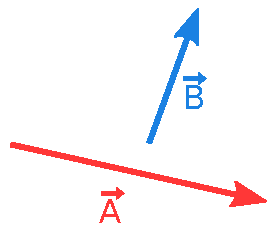
\includegraphics[scale=0.8]{Graphics/vectors/adding1}

Move them together head-tail and draw the sum as the vector between the ``total tail'' and ``total head'':
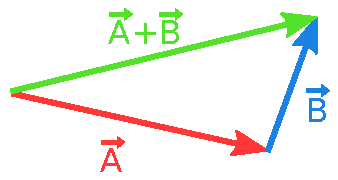
\includegraphics[scale=0.9]{Graphics/vectors/adding2}

This method works equally well with any number of vectors - just link them up tail-head as above; the sum vector will be the vector from the tail of the ``group'' to the head of the group, exactly as above.\\
The reason that we can do this is that vectors are completely characterized by their magnitude and direction - location in space is irrelevant. Two vectors with the same magnitude and direction are always equal, irrespective of their location. Therefore, we can move the vectors around to help us visualize vector addition.

So why does this method work? Well, imagine first travelling along $\vec{A}$, and then along $\vec{B}$. You would end up at $\vec{A}$ + $\vec{B}$. It really is that simple!

As for subtraction, one way to think about it is to \emph{add} the \emph{negative} vector instead, i.e. $\vec{a} - \vec{b} = \vec{a} + (-\vec{b})$. So what is $-\vec{b}$, exactly? It's simply the vector $b$ with the direction reversed. The magnitude is the same; the only difference is that you draw the arrow on the opposite side of the line.

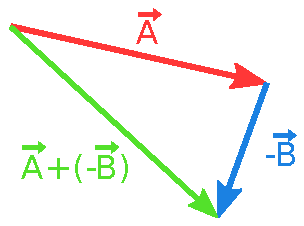
\includegraphics[scale=0.9]{Graphics/vectors/vectorsub}

Note that the vectors in the above graphic are the same vectors as in the addition example; however, the blue vector graphic is now $-\vec{b}$, which is then added to $\vec{a}$ to produce the result $\vec{a} - \vec{b}$.

That covers the basics of the graphical way to add and subtract vectors; what about the mathematical way? Well, in order to cover that, we need to first introduce the concept of vector components, and \emph{vector decomposition}.

What happens if we multiply a vector by a scalar (a dimensionless number)? Well, vectors work like numbers in that regard, in that $2 \cdot \vec{a} = \vec{a} + \vec{a}$. Draw that addition out on paper, and you'll see that the geometrical meaning is that the magnitude doubles, but the direction is unchanged.\\
As we saw above, when multiplying by negative numbers, the magnitude changes as appropriate, but the direction is flipped. $-3 \cdot \vec{a}$ would be a vector that is three times a big as $\vec{a}$, but points in the opposite direction. Multiplication by fractions (and even irrationals) work just as well, too.

\section{Vector components}

We can represent a vector as the sum of multiple vectors. In the most useful case, we can represent it as the sum of one vector ``per dimension'' the vector requires.\\
For a 2D vector in the Cartesian coordinate system, we can break a vector $\vec{A}$ into two vectors $\vec{A_x}$ and $\vec{A_y}$, such that the two vector components' directions are perpendicular; $\vec{A_x}$ points along the positive $x$ axis, while $\vec{A_y}$ points along the positive $y$ axis.

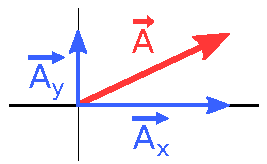
\includegraphics[scale=1.0]{Graphics/vectors/vectorcomponents}

Imagine moving $\vec{A_y}$ to the head of $\vec{A_x}$; if we draw the sum vector, we would get exactly $\vec{A}$. That is, $\vec{A} = \vec{A_x} + \vec{A_y}$.

We can also think of the magnitude of the partial vectors, $A_x$ and $A_y$. Those magnitudes represent how long the vector is in each dimension separately, and are very useful - more useful than the partial vectors themselves.

So \emph{why}, or where, is this useful? For one, when this technique is combined with unit vectors (below), it makes mathematical manipulation of vectors much easier. Vector decomposition can also be a powerful tool in solving physics problems, as it can break down problems in multiple dimensions to multiple smaller, one-dimensional problems, which are often easier to solve.

%\newpage

\subsection{Unit vectors}
Unit vectors are simple, but the concept is still very powerful. We define unit vectors to be vectors of magnitude 1 that point in the direction of their respective axes. The unit vector $\hat{i}$ (``i-hat``), points in the positive $x$ direction, while $\hat{j}$ points in the positive $y$ direction, and $\hat{k}$ in the positive $z$ direction. These unit vectors are also sometimes known as $\hat{x}$, $\hat{y}$ and $\hat{z}$, respectively. In addition, the ``hat'' suffix is sometimes called ``roof'', as in ``x roof''.

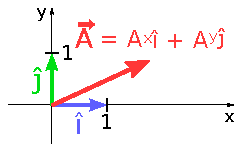
\includegraphics[scale=1.6]{Graphics/vectors/unitvectors}

Let's go back to the vector components above. The two components of $\vec{A}$ are both vectors, $\vec{A_x}$ and $\vec{A_y}$. We can write these components as the product of their magnitude (a scalar) and the unit vector in that direction (which is obviously a vector). Let's call the magnitude of vector $\vec{A_x}$  simply $A_x$.\\
Think of the vector $\vec{A_x}$ in the vector components figure as a longer version of the unit vector $\hat{i}$ - that is, it's the result of scalar multiplication of a magnitude, $A_x$, and the unit vector $\hat{i}$: $\vec{A_x} = A_x \hat{i}$\\
The same can be said for the component vector $\vec{A_y}$, which can be written as $A_y \hat{j}$.

Since we know that the sum of these two vectors equal $\vec{A}$, we now have
\[ \vec{A} = \vec{A_x} + \vec{A_y} \]
\[ \vec{A_x} = A_x \hat{i} \]
\[ \vec{A_y} = A_y \hat{j} \]
\[ \vec{A} = A_x \hat{i} + A_y \hat{j} \]

We have now written vector $\vec{A}$ as the sum of two separate, one-dimensional vectors. If we are working on a two-dimensional projectile motion problem, we can now calculate the motion along the x-axis as one problem, then calculate the motion along the y-axis as a separate problem, and then add the two together to get the combined motion. Doing so is generally much easier than solving the two-dimensional problem as-is.

We can also write that last equation ($\vec{A} = A_x \hat{i} + A_y \hat{j}$) as
\[ \vec{A} = \langle A_x, A_y \rangle \]
Here, we use a more compact notation, where the x and y components are listed, with the implicit meaning that me can construct the vector $\vec{A}$ by multiplying them by their respective unit vector, and adding the results.

%\newpage

\subsection{Vector decomposition}
Now that we know about vector components and unit vectors, let's apply these concepts, and also see how to actually do this decomposition mathematically. We've yet to see it from anything but a geometrical perspective. Sure, such perspectives are very useful for intuition, but in return, they are mostly useless for precise computation.\\
We can still use a picture to easier understand the mathematical decomposition, though:

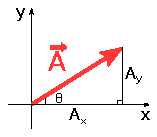
\includegraphics[scale=2]{Graphics/vectors/vectordecomp_trig}

Here, we see that $A_x$, $A_y$ and $\vec{A}$ form a right triangle.

Via the Pythagorean theorem, we see that
\[ |\vec{A}| = \sqrt{{A_x}^2 + {A_y}^2} \]

That is, the magnitude of the vector $\vec{A}$ is given by the sum of the squares of the component magnitudes.

If the vector were three-dimensional, we would simply add a ``$+ {A_z}^2$'' under the square root; the same goes for even higher dimensions.

However, while that is extremely useful, it doesn't help us \emph{find} $A_x$ and $A_y$ to begin with!\\
Let's stop stalling. Again, note how the three lines (if we consider the vector a line for now) form a right triangle. If we know the magnitude of the vector, i.e. the length of the hypotenuse, and the angle $\theta$ (theta) between the vector and the positive x axis, we can use trigonometry to find the components:

\[ \cos{\theta} = \frac{A_x}{|\vec{A}|} \]
\[ \sin{\theta} = \frac{A_y}{|\vec{A}|} \]

These come from the definitions of the sine and cosine functions - the cosine is the adjacent side ($A_x$) over the hypotenuse (the magnitude of $\vec{A}$), while sine is opposite ($A_y$) over hypotenuse.\\
We can now simply solve these equations for the components by multiplying both sides (of both equations) by the magnitude:

\[ A_x = |\vec{A}| \cos{\theta} \]
\[ A_y = |\vec{A}| \sin{\theta} \]

\subsection{Example}
Consider a vector with length/magnitude $|\vec{A}| = 5$ meters and angle $\displaystyle \theta = 30^{\circ} = \frac{\pi}{6}$ radians from the x axis. In other words, it's pointing ``to the right'' and slightly upwards, as seen from the origin.\\
In order to write this as a set of components, we can simply calculate the components as above:

\[ A_x = 5 \cos{\left( \frac{\pi}{6}\right) } = \frac{5 \sqrt{3}}{2} \approx 4.33 \text { meters} \]
\[ A_y = 5 \sin{\left( \frac{\pi}{6}\right) } = 2.5 \text { meters} \]

We can therefore write the vector as either of these forms (keeping in mind that we rounded the x value):
\[ \vec{A} = 4.33 \hat{i} + 2.5 \hat{j} \]
\[ \vec{A} = \langle 4.33, 2.5 \rangle \]

\section{Vector addition and subtraction, continued}
We now know what we need in order to talk about the mathematical way of vector addition and subtraction. Thankfully, once we've separated a vector into its components, addition and subtraction becomes incredibly easy!

Let's take the example of adding two vectors:
\[ \vec{a} = 5 \hat{i} + 3 \hat{j} \]
\[ \vec{b} = 2 \hat{i} - 1 \hat{j} \]
\[ \vec{a} + \vec{b} = (5 \hat{i} + 3 \hat{j}) + (2 \hat{i} - 1 \hat{j}) \]
\[ \vec{a} + \vec{b} = 7 \hat{i} + 2 \hat{j} \]

Yes, it's that easy - just add the parts separately, and you have the answer. Subtraction works as you would expect at this point. Let's try the more compact notation; the vectors used are the same as the ones in the addition example above.
\begin{align*}
\vec{a} = \langle 5, 3 \rangle\\
\vec{b} = \langle 2, -1 \rangle
\end{align*}
\begin{align*}
\vec{a} - \vec{b} &= \langle 5 - 2, 3 - (-1) \rangle\\
\vec{a} - \vec{b} &= \langle 2, 4 \rangle
\end{align*}

\section{The dot product / scalar product}
Now that we have addition and subtraction down, let's have a look at vector multiplication. There are two ways to multiply two vectors: the dot product, and the cross product.\\
The dot product gives a scalar result (a single number), and is therefore sometimes called the \emph{scalar product}, while the result of a cross product is a third vector.
Note that the two aren't simply different ways of doing the same thing, but fundamentally different operations, with completely different meanings and results.\\
The dot product is usually considered easier, so let's tackle that one first.

First off, notation. The name dot product comes from the notation used for the operation:
\[ \vec{a} \cdot \vec{b} \]

Before explaining the purpose of the dot product, let's go with the definitions and an example. It's rather easy to calculate, at least when you have the vector components.

Two definitions of the dot product, for two vectors with components $\vec{a} = \langle a_1, a_2, a_3 \rangle$ and $\vec{b} = \langle b_1, b_2, b_3 \rangle$, are:
\[ \vec{a} \cdot \vec{b} = a_1 b_1 + a_2 b_2 + a_3 b_3 \]
\[ \vec{a} \cdot \vec{b} = |\vec{a}| |\vec{b}| \cos{\theta} \]
Or, generally, for a vector with $n$ components/$n$ dimensions:
\[ \vec{a} \cdot \vec{b} = \sum_{i=1}^n a_i b_i = a_1 b_1 + a_2 b_2 + \cdots + a_n b_n \]

Let me just add one last definition before we look at this from a geometrical point of view:

\[ \vec{a} \cdot \vec{a} = |\vec{a}|^2 \]

Keeping in mind that the angle between a vector and itself must be 0, and that $\cos{(0)} = 1$, this should make sense if you believe the formulas above.

Therefore, the magnitude of a vector can also be written as:
\[ |\vec{a}| = \sqrt{\vec{a} \cdot \vec{a}} \]

Like vector addition, the dot product operation is commutative; that is, $\vec{a} \cdot \vec{b} = \vec{b} \cdot \vec{a}$. As we'll see later, however, the same is \emph{not} true for the cross product!

Now, if you've never seen the dot product before, I would assume you are a bit confused at this point. No worries - the above is meant as a ``reference'', not a tutorial. Let's get to the geometrical interpretation.

\subsection{Geometrical interpretation of the dot product}
Let's repeat the second definition of the dot product from above:
\[ \vec{a} \cdot \vec{b} = |\vec{a}| |\vec{b}| \cos{\theta} \]

Note that it's clear that the sign of the dot product is determined by (the cosine of) the angle and by that alone; the other terms are both magnitudes, which are always positive, by definition.\\
If the dot product is positive, the two vectors are pointing ``mostly'' in the same direction, i.e. the angle between them is less than 90 degrees; the angle is acute.
The dot product is zero if and only if the two vectors are perpendicular, as that's where the cosine term would be zero, and make the dot product zero as well.

%\newpage
And, if the angle is greater than 90 degrees, so that the vectors are pointing in different directions (with an obtuse angle between them), the dot product would be negative, as the cosine of the angle would be negative.

In a bit more concise form:
\[
\vec{a} \cdot \vec{b} =
	\begin{cases*}
	> 0 & \text{for $\theta < 90^\circ$, acute angle} \\
	  0 & \text{for $\theta = 90^\circ$, right angle} \\
	< 0 & \text{for $\theta > 90^\circ$, obtuse angle}
	\end{cases*}
\]

Now, let's look at this from a geometrical perspective, as promised.

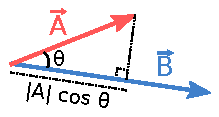
\includegraphics[scale=1.7]{Graphics/vectors/vectordot}

Here, we have two vectors, $\vec{A}$ and $\vec{B}$. We draw a line from $\vec{B}$, \emph{perpendicular} to $\vec{B}$, that meets $\vec{A}$ at the head. By definition, the angle between the line and $\vec{B}$ is 90 degrees.

Let's now use the definition of the cosine ($\displaystyle \cos \theta = \frac{\text{adjacent}}{\text{hypotenuse}}$) to find the length of the segment denoted by the dotted line, which we'll denote $|A_B|$, or ``the projection of $\vec{A}$ onto $\vec{B}$'':

\[ \frac{|A_B|}{|\vec{A}|} = \cos{\theta} \]
Solve for $|A_B|$ by multiplying both sides by the magnitude of $\vec{A}$:
\[ |A_B| = |\vec{A}| \cos{\theta} \]

Now we know, as the picture suggests, that the projection of $\vec{A}$ onto $\vec{B}$ is given by the magnitude of $\vec{A}$ times the cosine of the angle that separates the two vectors.\\
Now, remember the definition of the dot product:
\[ \vec{A} \cdot \vec{B} = |\vec{A}| \; |\vec{B}| \cos{\theta} \]
We can rearrange the terms to give:
\[ \vec{A} \cdot \vec{B} = |\vec{A}| \cos{\theta} \; |\vec{B}|\]
Using the identity just above, this is the same thing as:
\[ \vec{A} \cdot \vec{B} = |A_B| \; |\vec{B}|\]

So, we see that the geometrical interpretation of the dot product is, in one way to put it, the length that $\vec{A}$ goes in the direction of $\vec{B}$ (or the projection of $\vec{A}$ onto $\vec{B}$), times the magnitude of $\vec{B}$.\\
If this doesn't quite make sense, it will probably be easier to grasp when in actual use, such as when multiplying a force vector with a displacement vector to find work.

Another way (the same way, really) to think about it is this: imagine that the vector $\vec{B}$ is horizontal, i.e. parallel with the x axis, pointing to the right (the positive x axis).\\
Now, $|A_B|$ is just the x component of $\vec{A}$! Therefore, in general, we can think of $|A_B|$ as the ``B direction component'' of $\vec{A}$, so the dot product is the ``B direction component'' of $\vec{A}$ times the magnitude of $\vec{B}$.

\section{The cross product / vector product}
As the second naming suggests, this method of multiplying two vectors yields a third vector, namely one that is perpendicular to BOTH the vectors multiplied.\\
The notation used is, as the \emph{first} naming suggests, a cross:
\[ \vec{A} \times \vec{B} = \vec{C} \]

The cross product is only properly defined for 3- and 7-dimensional vectors. We will of course only work with the former in this course.

Okay, so we know that the cross product gives a third vector, that is perpendicular to both the vectors multiplied. It's also very important to know that the cross product operator is not commutative. That is,

\[ \vec{B} \times \vec{A} \neq \vec{A} \times \vec{B} \]
It is \emph{anticommutative}:
\[ \vec{B} \times \vec{A} = -(\vec{A} \times \vec{B}) \]

It also works alongside scalar multiplication, so that
\[ (r \vec{A}) \times \vec{B} = \vec{A} \times (r \vec{B}) = r(\vec{A} \times \vec{B}) \]

Okay, okay, enough with the side-definitions. What is the definition of the cross product?\\
Well, as previously, there are two definitions we'll use: one that uses magnitude and angle, and one that uses vector components. The latter is rather complex, but here's the first one, to begin with: \subsection{Definition: Magnitude and angle}

\[ \vec{A} \times \vec{B} = |\vec{A}| \; |\vec{B}| \; \sin{\theta} \; \hat{n} \]
This is, you might note, very similar to the dot product, except it has a sine rather than a cosine, and also has a direction (we'll get to that soon), since it's a vector.\\
If we want just the magnitude of the cross product, it's eerily similar to the dot product:
\[ |\vec{A} \times \vec{B}| = |\vec{A}| \; |\vec{B}| \; \sin{\theta} \]
The sine instead of the cosine is now the only difference.

One way to think about it is that the \emph{dot} product measures ``how parallel'' two lines are. When completely parallel, the dot product is at its maximum. (Mathematically, the $\cos{\theta}$ term is 1, its maximum, when $\theta = 0$, i.e. the angle between the two is 0, i.e. they are completely parallel.)\\
The dot product is then zero when the vectors are perpendicular (not parallel at all), and negative when they point in different directions ($\theta > 90^\circ$).

What about the \emph{magnitude of} the cross product (not just the cross product itself!)? It's pretty much the opposite: you can think of it as measuring ``how perpendicular'' two vectors are. With two fully parallel vectors, the cross product equals zero (the angle $\theta = 0$, and $\sin{(0)} = 0$). When they are perpendicular, the cross product is at its maximum, since $\sin{(90^\circ)} = 1$.

Okay, so that covers the magnitude, what about the direction, $\hat{n}$? As the hat/roof suggests, that is a unit vector... but in what direction? Hang on; we'll discuss that in the geometrical interpretation, after the component definition.

\subsection{Definition: components}

The second definition, using components - in its worst possible form (it'll get better soon) - is:
\[ \text{For } \vec{C} = \vec{A} \times \vec{B}\text{:} \]
\[ \vec{C} = (A_y B_z - A_z B_y) \hat{i} + (A_z B_x - A_x B_z) \hat{j} + (A_x B_y - A_y B_x) \hat{k} \]
Oh dear. Thankfully, there are ways to remember the above. First, what we do - for the mnemonic to work - is to rename the variables, and instead compute
\[ \vec{A} = \vec{B} \times \vec{C} \]
Without this change, the mnemonic is probably \emph{harder} to remember than the above mess, so go with me.\\
After that change, we write the component equations separately, instead of all on one line. The sums-of-products are the same as above, though, if we account for the variable renames:
\[ A_x = B_y C_z - B_z C_y \]
\[ A_y = B_z C_x - B_x C_z \]
\[ A_z = B_x C_y - B_y C_x \]

Still awful. Heck, it might just look harder like this! Don't panic - there's a pattern: {\bf XYZZY}.\\
Note that the subscripts of the first equation spell XYZZY, and that the vector order is alphabetical for all equations ($A_* = B_* C_* - B_* C_*$).\\
That makes the first one relatively easy (compared to memorizing the entire thing), but what about the rest?\\
A-ha! Here's the pattern: to convert from the first equation to the second, ``increase'' the subscript by one letter; if at z, go back to x. That is, $A_x$ becomes $A_y$ (one letter ahead), $A_y$ becomes $A_z$ (one letter ahead), and $A_z$ wraps around and becomes $A_x$; the same thing applies to the B and C components.\\
The same method is used to convert from the second to the third equation. Have a close look at them and make sure you realize this is true!

As an additional sanity check, note that the reverse of the first subscript pair is the one you then subtract: yz - zy, zx - xz and xy - yx. (Look at the subscripts in the three equations again if you don't get what I mean.)

Since $\vec{C}$ is supposed to be perpendicular to both $\vec{A}$ and $\vec{B}$, we can use the dot product to check whether our answer appears to be correct or not. Remember that the dot product is always zero for two perpendicular vectors - so we could check our work by testing that the two dot products $\vec{A} \cdot \vec{C}$ and $\vec{B} \cdot \vec{C}$ are both zero. If either or both is \emph{not} zero, the cross product calculation was done incorrectly. If both \emph{are} zero, that doesn't guarantee that the answer is correct, however. More on that later (there are two vectors perpendicular to both $\vec{A}$ and $\vec{B}$: $\vec{C}$ and -$\vec{C}$).

%\newpage
\subsection{Geometrical interpretation of the cross product}
Let's try to make sense of all the above.\\
We can imagine a parallelogram plane in 3D space, with two sides $\vec{A}$ and $\vec{B}$. This is certainly one of those times where an image is worth (more than) a thousand words:

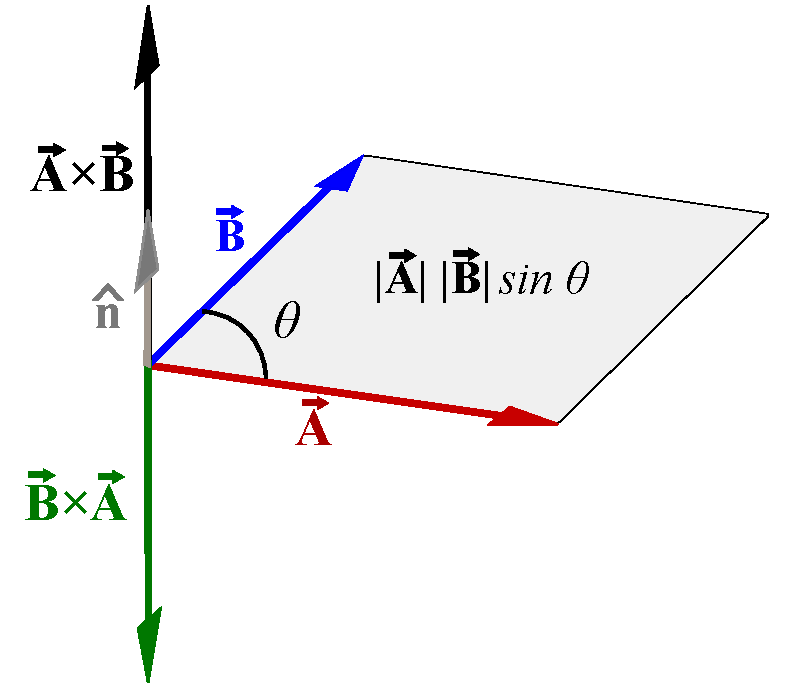
\includegraphics[scale=0.5]{Graphics/vectors/cross-product-with-area}

(Image license is CC0. By Wikimedia user Svjo; modified by me.)

Here, we can see several key things:
\begin{itemize*}
\item The area of the parallelogram is the magnitude of the cross product, $|\vec{A}| \; |\vec{B}| \; \sin{\theta}$ (this is one of the ways to calculate the area of a parallelogram).
\item The unit vector $\hat{n}$ (and therefore the cross product) is indeed perpendicular to \emph{both} $\vec{A}$ and $\vec{B}$; another way of saying this is that it's perpendicular to the plane formed by $\vec{A}$ and $\vec{B}$.)
\item $\vec{B} \times \vec{A}$ points in the opposite direction as $\vec{A} \times \vec{B}$ does, since $\vec{B} \times \vec{A} = -(\vec{A} \times \vec{B})$. (Remember that the negative of a vector is a vector pointing in the opposite direction, i.e. with the arrowhead on the other side of the line.)
\end{itemize*}

However, we also see a problem: if both the upwards-pointing vector $\vec{A} \times \vec{B}$ and the downwards-pointing vector $\vec{B} \times \vec{A}$ are perpendicular to both $\vec{A}$ and $\vec{B}$, and they are (obviously!) not equal... how do we know which of the two to use? How do we identify which is which?

We'll have to use a rule known as the \emph{right-hand rule} for this.\\
The right-hand rule is often tought in different ways, all with the same end result. The way I prefer is one using your whole right arm, simply because because I find it easier.\\
The rule is this: if your entire right arm points along the first vector ($\vec{A}$), angle your index through pinky (four fingers) in the direction of the second vector ($\vec{B}$); if this means you have to turn your arm, do so.\\
Now, with your arm pointing along vector $\vec{A}$ and your fingers pointing along vector $\vec{B}$, extend the thumb straight out. Your thumb should now be perpendicular to both $\vec{A}$ and $\vec{B}$, and point along $\vec{A} \times \vec{B}$ (and not $\vec{B} \times \vec{A}$ - try swapping the arm and the finger vectors, and you'll find that the result is the thumb pointing in the opposite direction!).

That is:

\begin{itemize*}
\item Right hand/entire arm points parallel to $\vec{A}$
\item Fingers are curled to point parallel to $\vec{B}$
\item Thumb now points parallel to $\vec{A} \times \vec{B}$ (perpendicular to both $\vec{A}$ and $\vec{B}$).
\end{itemize*}

Note that this is only true for certain coordinate systems, namely \emph{right-handed} ones. These are the ones used by all sane persons in physics, and the only ones used in this document.

One useful definition to test whether a system is right-handed or not, is that this SHOULD be true:

\[ \hat{i} \times \hat{j} = \hat{k} \]
If the above is false for your coordinate system (i.e. you get $-\hat{k}$ instead), your coordinate system is left-handed and simply won't work according to the definitions generally used in physics!

\part{8.01x ``Classical Mechanics''}

\setcounter{chapter}{0}

\chapter{Week 1}

\section{Lecture 1: Units, dimensions and scaling arguments}

The lecture begins with a quick intro to units, followed by a movie showing 40 orders of magnitude (from inside a proton, to a perspective 100 million lightyears from Earth).

After that, we begin talking about dimensional analysis and the metric system.
The three SI base units, and their respective dimensions, are introduced: the meter (m) for measuring length [L], the second (s) for measuring time [T] and the kilogram [kg] for measuring mass [M].\\
We use the square brackets to notate that we are not talking about a \emph{unit}, but a \emph{dimension} - such as the three shown above (length, time, mass), or speed, acceleration, temperature, charge, etc.\\
One dimension can have many units (meters, yards, kilometers, miles and light-years all describe length), but one unit always describes exactly one dimension. (If it were not so, we could perhaps measure temperature in meters, or length in amperes!)

As an important side note, keep in mind that capitalization is extremely important in physics: 1 mm is 1/1000 of a meter, a very short distance, while 1 Mm is a million meters, or 1000 kilometers - a distance larger than many countries. The same goes for units: k means kilo (the prefix for 1000), while K means Kelvin, a unit of absolute temperature. Capital $G$ is the symbol for the gravitational constant (about $6.67 \cdot 10^{-11} \text{ N(m/kg)}^2$), while a lowercase $g$ is the symbol for the gravitational acceleration near Earth, about $9.8 \text{ m/s}^2$. The two are related, but still completely different, so they must not be confused for one another.

Many other units can be described as combinations of the three base units shown above, for example:

\begin{equation}
 \text{[speed]} = \frac{\text{[L]}}{\text{[T]}}
\end{equation}

All units of speed are in length per time - meters per second, kilometers per hour, inches per year, etc. Therefore, we say that the \emph{dimension} of speed is the dimension of length per time, as shown above in a more mathematical notation.

Other examples are:

\begin{equation}
 \text{[volume]} =\text{[L]}^3
\end{equation}
\begin{equation}
 \text{[density]} = \frac{\text{[M]}}{\text{[L]}^3}
\end{equation}
\begin{equation}
 \text{[acceleration]} = \frac{\text{[L]}}{\text{[T]}^2}
\end{equation}

The last one may seem strange if you have not studied physics before - an example of a unit of acceleration is meters per second squared, or meters per second per second ($m/s^2$ or $(m/s)/s$). It's quite simple though, once you get past the wording of it.\\
When measuring a change in something, we always add another "per second" (or another unit of time), so when the unit we are measuring the change in is already meters per second, we get meters per second per second.\\
For example, a car might start out at 0 m/s (standing still), and be moving at 5 m/s one second later. In that case, the car's average acceleration is 5 meters per second per second.

\subsection{Uncertainty, and an experiment}
Prof. Lewin stresses very strongly: ``Any measurement you make without knowledge of its uncertainty is \emph{meaningless}''. He repeats this a few times throughout the lecture.

Using two rulers accurate to about $\pm$ 1 mm, he measures a student first standing up, and then lying down -- after measuring an aluminum bar, to show that the two rulers agree. They do, within 1 mm - the uncertainty.
The results of the experiment are a bit surprising: the student was about 2.5 cm $\pm$ 0.2 cm taller lying down! The reason being that gravity compresses our bodies slightly when standing up, while that effect would be gone lying down (since gravity then acts perpendicular to our length).

Because of the small uncertainty, compared to the relatively large height difference, we can be sure that the student indeed was taller lying down. Had the uncertainty of the measurement instead been $\pm 3$ cm, how could we know? The two values $185.7$ cm and $183.2$ cm are indistinguishable from each other if measured with a meter stick where the uncertainty is $\pm 3$ cm! The first could be anything between 182.7-188.7 cm, while the second could be anything from 180.2-186.2 cm. There is considerable overlap, which means the two could indeed be equal -- we could only know by making a more accurate measurement.

Calculating uncertainty properly can be quite complex, and the correct methods will not be taught or used in this class, as it is simply out of the scope. Instead, we use simplified methods, ``poor man's'' as the professor called them.

\subsubsection{Uncertainty in addition and subtraction}

For addition and subtractions, it couldn't be much easier: the uncertainty of the sum or difference is simply the sum of the two uncertainties:

\begin{equation}
 (A \pm a) + (B \pm b) = (A + B) \pm (a +b)
\end{equation}
\begin{equation}
 (A \pm a) - (B \pm b) = (A - B) \pm (a +b)
\end{equation}

You can find this result by calculating with the extremes. For example, for adding $1.5 \pm 0.003 \text{ m} + 3 \pm 0.005 \text{ m}$:

\begin{equation}
\text{min} = 1.497 \text{ m} + 2.995 \text{ m} = 4.492 \text{ m}
\end{equation}
\begin{equation}
\text{max} = 1.503 \text{ m} + 3.005 \text{ m} = 4.508 \text{ m}
\end{equation}

Both results are $0.008$ m away from $3 + 1.5 = 4.5$, and so the uncertainty is $\pm 0.008$ m, the sum of the two uncertainties.  
If we use the same method where we subtract, we will find the same result: the uncertainties \emph{add}, and the results will differ from the simple difference by $+0.008$ and $-0.008$, respectively.

\subsubsection{Uncertainty in multiplication and division}

First, keep in mind that some numbers are exact. If we multiply a length by 2 -- a constant, not a measurement -- then the length and the uncertainty are both multiplied by 2 exactly. No further work is necessary.\\
If the two are measurements, however, care needs to be taken.

One way to get a \emph{rough} uncertainty value when dividing is to choose the largest and smallest values, respectively, for the numerator and denominator, and then subtract the nominal value from that.\\
As an example, let's say we want to calculate the approximate gravitational acceleration of the Earth based on measurements of the time for an object to fall from a certain height. The equation used is

\begin{equation}
 g = \frac{2 h}{t^2}
\end{equation}

The 2 here is an exact value, so we don't need to worry about it.\\
If the height is $\SI{3.000(3)}{m}$ and the time taken is $\SI{0.781(2)}{s}$, we then find:

\begin{equation}
g = \frac{2\cdot\SI{3.000}{m}}{(\SI{0.781}{s})^2} \approx \SI{9.8367}{m/s^2} \approx \SI{9.84}{m/s^2}
\end{equation}

We can then calculate the uncertainty as mentioned above. For the numerator, we add the $+ 0.003$ m, and in the denominator, we subtract the $- 0.002$ s. Finally, we subtract the nominal value that we found above.

\begin{equation}
\text{error} = \frac{2 \cdot \SI{3.003}{m}}{(\SI{0.779}{s})^2} - g = \SI{9.8971}{m/s^2} - \SI{9.8367}{m/s^2} = 0.0604 \approx \SI{0.06}{m/s^2}
\end{equation}

There has not yet been an example with multiplication used in the course, but I would assume that you still try to find the maximum possible value (by choosing the maximum for both terms) and then subtract the nominal value, just as above.

\subsection{Scaling arguments and Galileo Galilei}

Long ago, Galileo Galilei asked himself: why are the mammals the sizes they are, and not much bigger? The short version of a possible answer he came up with is that if they were more massive, their bones would break. Below is a more detailed analysis of what he might have thought about.

Say we have a mammal. It has a size $S$ - very roughly defined, of course: there is no single length that defines the actual size of an animal properly. Let's just say that a mouse is perhaps 10 cm (plus the tail), and a horse is couple of meters -- and let's not worry about the details.

The animal has a thigh bone, or \emph{femur}, of length $\ell$, and a thickness $d$ (at the thinnest point). The cross-sectional area at that point is $A$. We can safely say that $A \propto d^2$ (A is proportional to d squared): doubling $d$ will multiply the cross-sectional area by 4.
We call the mass of the animal $m$.

\begin{center}
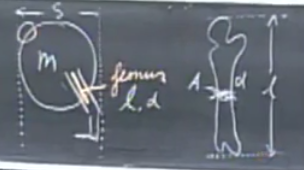
\includegraphics{Graphics/femur}
\end{center}

Let's now have a look at a scaling argument.\\
We assume that the length of the femur scales linearly with the size of the animal. That is, if the animal is twice as large as another, its femur will be twice as long as the other animal's femur. A reasonable assumption, one would think.

We then assume that the animal's mass is proportional to the cube of the size -- also very reasonable, as the size to the third is related to the animal's volume. Twice the volume, twice the mass, assuming the density is similar, of course.\\
Because of the previous relationship ($\ell \propto S$), this also implies that the mass is proportional to the length of the femur cubed. In mathematical notation, so far we have:

\begin{align}
 \ell &\propto S \label{eq:lproptoS}\\
 m &\propto S^3 \propto \ell^3 \label{eq:mproptoS3}
\end{align}

The \emph{pressure} on the femur is proportional to the weight of the animal, divided by the femur's cross sectional area. The weight (which the course will talk about later) is proportional to the mass, and as stated earlier, A is proportional to $d^2$, so we have

\begin{equation}
 \text{pressure} \propto \frac{m}{A} \propto \frac{m}{d^2}
\end{equation}

Because the bones will break if the pressure on them is too great, $m$ cannot increase without $d^2$ increasing by the same factor, if the animal is fairly close to the breaking limit already. This is key in this argument.

Because of this, we find
\begin{equation}
m \propto d^2 \label{eq:mproptod2}
\end{equation}

... or the above cannot be true.
Combining equation \eqref{eq:mproptoS3} with equation \eqref{eq:mproptod2} just above, we find

\begin{equation}
 d^2 \propto \ell^3
\end{equation}
or, taking the square root of both sides,
\begin{equation}
 d \propto \ell^{3/2} \label{eq:dproptoell32}
\end{equation}

The above is the result we have been looking for. What this means is that if we have two animals, one being 10 times larger than the other ($S$ being 10 times larger, which implies $\ell$ being 10 times larger via \eqref{eq:lproptoS}, via the above relation, the diameter of the femur $d$ must be $10^{3/2} \approx 32$ times greater!\\
If we compare e.g. a mouse and an elephant, the difference in size being perhaps 100 times, via the same relationships, $d$ must be $100^{3/2} = 1000$ times greater for the elephant!

Galileo Galilei may have thought this to be a good explanation as to why mammals are the size they are, and not much bigger: much larger animals would have bones so large, that they barely consist of anything else than bones to hold their weight up. Let's see if this appears to be correct by making some calculations on actual measurements of animal femurs.

If we take equation \eqref{eq:dproptoell32} and divide both sides by $\ell$, we find

\begin{equation}
\frac{d}{\ell} \propto \sqrt{\ell}
\end{equation}

This is then plotted from the professor's measurements of the bones. If the above is correct, we would expect that if $\ell$ is 4 times greater (such as a horse vs a raccoon), $d/\ell$ should be $\sqrt{4} = 2$ times greater.

The professor then showed the result of the experiment, by measuring these values ($d$ and $\ell$) for bones from various animals: a mouse, an opossum, a raccoon, an antelope, a horse, and an elephant. There was no evidence that the ratio of $d/\ell$ was different as we would have been expected. Even for the case of a mouse vs an elephant, where the difference in size (and thus $\ell$) would be about a factor of 100, so that we expect $d/\ell$ for the elephant to be about 10 times greater than for the mouse, we find less than a factor of two!\\
Similar relationships were shown between all animal sizes: in no case was $d/\ell$ significantly different, as the hypothesis predicted. It looks like we, and Galilei, must admit defeat. The hypothesis simply doesn't hold up to experiment!

\subsection{Dimensional analysis}

Let's now look at some basic kinematics (the physics of motion) and dimensional analysis in closer detail.\\
We drop an object, such as an apple, from a height $h$, and use a stopwatch to measure the time $t$ before it hits the ground. How does the time $t$ relate to the height $h$?

We can assume that the time is proportional to the height, to some unknown power, which we will call $\alpha$:

\begin{equation*}
 t \propto h^\alpha
\end{equation*}

The mass of the apple might matter, so we might expect to find it to be proportional to the mass to some unknown power $\beta$:

\begin{equation*}
 t \propto h^\alpha m^\beta
\end{equation*}

Finally, it might be related to the Earth's gravitational acceleration $g$ (not to be confused with the gravitational constant $G$; both of these will be introduced properly later in the course):

\begin{equation}
t \propto h^\alpha m^\beta g^\gamma
\end{equation}

We can now start trying to figure this out. We know that the left-hand side has the dimension of time, [T]. This means that the product on the right-hand side must also have the dimension of time. Using the dimensional analysis notation, we must have

\begin{equation}
 \text{[T]}^1 = \text{[L]}^\alpha \text{[M]}^\beta \left( \frac{\text{[L]}}{\text{[T]}^2} \right)^\gamma 
 \end{equation}
 ... where we have simply replaced the variable names with their respective dimensions, the dimension of $h$ being length, $m$ being mass, and $g$ being acceleration (length per time${}^2$).
 
 We can now start working. There is only one [M] in this equation, and it's on the right-hand side. There is no possible way to get it to cancel out with anything else, so $\beta$ must be 0 so that it disappears ``by itself'', so to speak.
 
 We have two [L] on the right hand side, but there is no [L] on the left-hand side. That means that the two must cancel each other out, in one way another. That is,
 
\begin{equation*}
 \alpha + \gamma = 0
\end{equation*}

must be true.

Finally, we have [T] to the power one on the left-hand side, and to the power $-2\gamma$ (since it is in the denominator, it is negative) on the right-hand side, and the two must be equal. All in all, we find

\begin{align*}
\beta &= 0\\
\alpha + \gamma &= 0\\
-2\gamma &= 1
\end{align*}

We can solve the last equation for $\gamma$, and stick that value into the second equation, to find the final answers:

\begin{align*}
-2\gamma &= 1\\
\gamma &= -\frac{1}{2}
\end{align*}

\begin{align*}
\alpha - 1/2 &= 0\\
\alpha = \frac{1}{2}
\end{align*}

And, so, we find these values, and these relationships with the variable names we had chosen earlier:

\begin{align}
t &\propto h^{1/2} g^{-1/2} \\
t &\propto \sqrt{\frac{h}{g}}
\end{align}

Since the meaning of a proportionality is that some (still unknown) constant multiplies the value, we can write this as an equality with an unknown constant $C$:

\begin{equation}
 t = C \sqrt{\frac{h}{g}}
\end{equation}

So, since the time is proportional to the square root of the height, we can tell than if we drop an object first from 2 meters, and then from 8 meters, it will take twice as long to fall the second time, despite the distance being 4 times as long (because $\sqrt{4} = 2$).

\subsection{An experiment}

This is then put to the test in the lecture, by dropping apples, and timing their fall. One drop was from 3 meters, $\pm 0.003$ meters, while the second was from 1.5 meters, also with $\pm 0.003$ meters as the uncertainty.

The ratio between the two is easily calculated as 2, but what about the uncertainty? If the numerator were $3.003$ m and the denominator $1.497$ m, those would give the largest ratio possible with the uncertainty of $\pm 0.003$. The result of that division is $2.006$, so we consider the uncertainty to be $0.006$:

\begin{equation}
 \frac{h_1}{h_2} = \frac{3.000 \pm 0.003 \text {m}}{1.500 \pm 0.003 \text{ m}} = 2.000 \pm 0.006
\end{equation}

Note that because this is a ratio between two lengths, the end result has no dimension and thus no unit.

Knowing this ratio, we can now predict the ratio between the fall times. Since the ratio between the heights is 2, and the time is proportional to the square root of the height, the ratio between the fall times should be about $\sqrt{2}$. Then there's that uncertainty again. We can use the same method to find the smallest possible and the largest possible result by calculating $\sqrt{2+0.006}$ and $\sqrt{2-0.006}$ and will find an uncertainty of about $\pm 0.002$. That gives us

\begin{equation}
 \frac{t_1}{t_2} = \sqrt{\frac{h_1}{h_2}} = 1.414 \pm 0.002 \label{eq:applepred}
\end{equation}

So, the above is our \emph{prediction}, and we have a set-up with the apple fall times being measured automatically. Let's see the results!

The apple falling from 3 meters $\pm 3$ mm took $0.781 \pm 0.002$ seconds to fall. The apple falling from 1.5 meters $\pm 3$ mm took $0.551 \pm 0.002$ seconds to fall.

If we then calculate the ratio between the two times, we find

\begin{equation}
\frac{0.781 \pm 0.002}{0.551 \pm 0.002} = 1.417 \pm 0.008
\end{equation}

... which is in agreement with the prediction in \eqref{eq:applepred} when we consider the uncertainties in our measurements. \emph{Physics works}, as Prof. Lewin would say.\\
As far the uncertainty of the above result goes, I get $\pm 0.009$ when calculating the same way as before. However, as mentioned before, this method is not truly correct, and the truly correct way is out of the scope of this course, so such a small difference does not matter.\\
As long as the uncertainty is 0.001 or more, the results can agree with each other.

\section{Lecture 2: Introduction to Kinematics}

\subsection{Distance vs displacement and velocity vs speed}

In everyday English, speed and velocity are usually used as synonyms. In physics, however, the two are very different, and it's important to understand the difference.\\
We can define the two as

\begin{align}
 \text{speed} &= \frac{\text{distance travelled}}{\text{time taken}}\\
 \text{velocity} &= \frac{\text{displacement}}{\text{time taken}}
\end{align}

On first glance, the two may appear to say the same thing, but they don't.\\
There is an important difference between the terms \emph{distance travelled} and \emph{displacement}. The first is a scalar, and is always positive (if not zero, if you have been standing still the entire time) and is equal to what a car's odometer would display.\\
Displacement, however, is a \emph{vector} (see Part I on vector mathematics, or lecture 3). It is the distance between the starting point and the ending point - which may be zero, if you've travelled back to the start.\\
The displacement vector, like all vectors, also has a direction, which is defined as pointing from the starting point to the ending point.\\
With this in mind, it should be clear that the distance travelled must \emph{always} be greater than or equal to the displacement. Anything else would require teleportation!

Now, consider the case where we travel 1 km due north, turn around, and travel 1 km due south. We have travelled 2 km, but we are still standing exactly where we started! In other words, the displacement is zero. Using the above definitions, our average \emph{velocity} for the entire journey was \emph{zero} -- zero displacement divided by any measured time is zero.\\
The average \emph{speed}, on the other hand, is guaranteed to be positive, and can be found by dividing the 2 kilometers travelled by the time the journey took.

There is another difference between the two: speed is a scalar, that is, a regular number like any other. Velocity, on the other hand, like displacement, is a vector.\\
The average speed for the first half of the journey (right where we turned around) might have been 10 m/s, while the average velocity at that point might have been 10 m/s to the north.

Vectors are introduced properly in the first part of these notes, and in the next lecture of the course as well.

\subsection{Kinematics}

\begin{center}
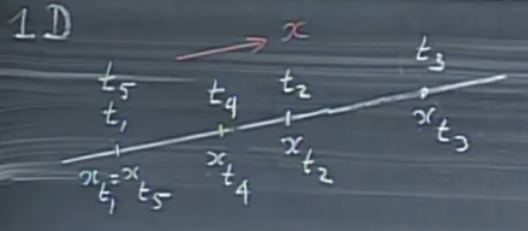
\includegraphics[scale=0.75]{Graphics/1d-motion}
\end{center}

The increasing direction of $x$ is as shown. An object moves along this line, first towards the right, then shortly after reaching the point $x_{t3}$ at  $t = t_3$, it reverses and moves back, until it is at $x_{t1} = x_{t5}$, where it started.

We can now introduce a definition for the \emph{average velocity} of this object between two times $t_1$ and $t_2$ as the following:

\begingroup
\large
\begin{equation}
 \overbar{v}_{t_1 t_2} = \frac{x_{t2} - x_{t1}}{t_2 - t_1}
\end{equation}
\endgroup

This should make some intuitive sense -- the numerator is just the distance between the two points (the \emph{displacement}), while the denominator is the time that has passed. Displacement over time gives us the \emph{average velocity}.

If we consider the average velocity between times $t_1$ and $t_5$, the answer is zero, because the position is the same for the two times, and so we have zero divided by the time taken, which is of course simply zero.\\
Between e.g. times $t_2$ and $t_4$, the velocity is \emph{negative}, which indicates we have moved in the \emph{opposite direction} of the positive $x$ axis.\\
The average velocity can be positive, zero or negative, depending on the positions involved.\\
The average \emph{speed}, however, is \emph{always} positive or zero. The average \emph{velocity} is still zero, because the distance between the starting point and the ending point is zero.

\begin{center}
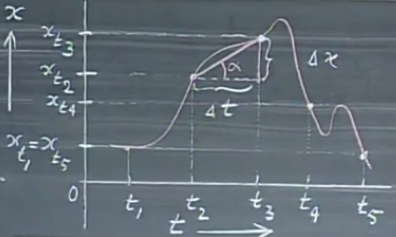
\includegraphics[scale=0.75]{Graphics/1d-motion-graph}
\end{center}

Here, we see a different way of notating what is really the same thing as we have above. If we call a difference in time $\Delta t$, and a difference in $x$ position $\Delta x$, we can find the average velocity as

\begin{equation}
 \overbar{v} = \frac{\Delta x}{\Delta t}
\end{equation} 

This is simply a different way of notating what we already had. Be careful with signs, though - if you take the first $x$ value in the middle, and the second from the right, be sure to take the $t$ values in the same order, or you will get the negative of the correct answer. In other words, your average velocity will be in the opposite direction of the actual movement.

Also shown above is the angle $\alpha$, that we can find between two arbitrary points. When $\alpha > 0$, as above (it's pointing upwards), the average velocity is positive. If it is instead negative, as it would be between $t_4$ and $t_5$, the average velocity is negative.

\subsubsection{Instantaneous velocity}

Since the definition of velocity we've seen thus far is only an average between two points in time, what is the meaning of instantaneous velocity (which is usually what we mean by ``velocity'' unless otherwise specified)?\\
Conceptually, the answer is that it is still an average, only that we move the two position measurements closer and closer together in time, until the time between them is zero.

Mathematically, velocity is the first \emph{derivative} of position.
We could write it as

\begingroup
\large
\begin{equation}
 v_t = \lim_{\Delta t \to 0} \frac{x_{t + \Delta t} - x_t}{\Delta t} = \frac{dx}{dt} = x'(t) = \dot{x}
\end{equation}
\endgroup

The last three are just three different ways of writing the same thing: the first derivative of $x$ with respect to $t$. Leibniz' notation looks like a fraction; Lagrange's notation uses the prime symbol (apostrophe) to indicate a derivative, and finally Newton's notation uses a dot above to signify the first time derivative. (In other words, the dot notation is used almost exclusively when the function is differentiated with respect to time, so the $t$ is implicit.)

As for speed, we can simply define instantaneous speed as the absolute value of the instantaneous velocity. In other words, if the velocity has a minus sign, remove it. If not, the two are equal.

\subsection{Calculating the average speed of a bullet}

Using an electronic, an experiment was set up to measure the speed of a bullet. The bullet is fired from a rifle, and breaks a wire, at which point the timing starts. Soon thereafter, the same bullet breaks another wire, at which point the timing stops.

Using a measurement of the distance, and a measurement of the time taken, we can calculate the average speed.

The distance was measured to be $148.5 \pm 0.5$ cm, that is, $1.485 \pm 0.005$ m.\\
The time taken was measured as $5.8 \pm 0.1$ ms, which equals, $0.0058 \pm 0.0001$ s.

The average speed is then

\begin{equation}
v_{avg} = \frac{\SI{1.485}{m}}{\SI{0.0058}{s}} = \SI{256}{m/s}
\end{equation}

The relative error in the timing can be calculated as 

\begin{equation}
\text{relative error} = \frac{\SI{0.1}{ms}}{\SI{5.8}{ms}} \cdot 100\% = 1.7\% 
\end{equation}

The uncertainty in the average speed can then be estimated. As the lecture question hints, we will ignore the uncertainty due to error in the distance measurement, because the timing error is much greater.

We can use the simple way introduced previously to find an approximate uncertainty:

\begin{equation}
\text{error} = \frac{1.485 \text{ m}}{0.0058 - 0.0001 \text{ s}} - \SI{256}{m/s} = \SI{4.5}{m/s}
\end{equation}

(We would add $+0.005$ m at the top, if we didn't choose to ignore the uncertainty it that measurement.)\\
Alternatively, we could have simply used the 1.7\% relative error we found above.\\
So in short, we can specify the average speed of the bullet as

\begin{equation}
v_{avg} = 256 \pm 4.5 \text{ m/s}
\end{equation}

\subsection{Acceleration}

Just as velocity is the change in position, acceleration is the change in \emph{velocity}. We can use an equation that looks extremely similar to find the \emph{average} acceleration $a$:

\begingroup
\large
\begin{equation}
 \overbar{a}_{t_1 t_2} = \frac{v_{t2} - v_{t1}}{t_2 - t_1}
\end{equation}
\endgroup

The dimension of acceleration, as mentioned previously, is length per time${}^2$, or [L] [T]${}^{-2}$, with $\text{m/s}^2$ being the most common unit, at least in this course.

Just as before, we can simplify this by using delta notation, with the same caveat: make sure to use the correct signs, or the result may end up incorrect.

\begin{equation}
\overbar{a} = \frac{\Delta v}{\Delta t}
\end{equation}

As an example, let's use the following lecture question. We define the direction of increasing $x$ as upwards (towards the sky). A tennis ball is thrown towards the ground at a velocity of about $\SI{-5}{m/s}$ - i.e. the speed is 5 m/s, downwards. It is in contact with the ground for about 1/100 second, after which it is moving at $\SI{+5}{m/s}$, i.e. upwards.\\
What is the average acceleration of the tennis ball?

Well, we have the formula above, so this should be fairly easy!

\begin{equation}
 \overbar{a_{ball}} = \frac{\SI{5}{m/s} - (\SI{-5}{m/s})}{\SI{0.01}{s}} = \frac{\SI{10}{m/s}}{\SI{0.01}{s}} = \SI{1000}{m/s^2}
\end{equation}

Keeping the signs in mind, we end up with a positive value for the acceleration, which has a ridiculous magnitude - over 100 times the Earth's gravitational acceleration.

The professor adds another example of acceleration. There is a limit to the amount of acceleration things can tolerate before they break. He used examples of tomatoes and eggs, also thrown to the ground at 5 meters per second.\\
The impact time will probably be much greater (perhaps 1/4 second), and the change in velocity will be only 5 m/s rather than 10, as neither the egg nor the tomato would bounce back up.\\
Despite that, clearly, both would break, even though the acceleration is a more modest $20 \text{ m/s}^2$ or so.

The next example was that of a human skull on a marble floor, from a Sherlock Holmes movie. Even at a relatively small velocity, a skull hitting such a hard floor, with no ``give'', the impact time would be extremely short. Since the impact time is in the denominator, a shorter time will result in a higher acceleration, and a skull can break despite the low speeds involved. 

\subsubsection{Instantaneous acceleration}

Just as we did with velocity, we now want a way to calculate the acceleration at a given instant, rather than the average between two measurements. We do this in exactly the same way: we find the first time derivative of the velocity.

\begingroup
\large
\begin{equation}
 a_t = \lim_{\Delta t \to 0} \frac{v_{t + \Delta t} - v_t}{\Delta t} = \frac{dv}{dt} = \frac{d^2x}{dt^2} = \ddot{x}
\end{equation}
\endgroup

We could also write this as $x''(t)$ or $v'(t)$, but I wanted to reduce the amount of clutter above somewhat.\\
Since acceleration is the time derivative of velocity, and velocity itself is the time derivative of position, acceleration is the \emph{second} time derivative of position, as shown above.

\subsection{General forms for one-dimensional motion}

We can write equations for the position and velocity in one-dimensional motion in such a way that they can be used for \emph{any} one-dimensional motion with a constant acceleration:

\begin{align}
x(t) &= x_0 + v_0 t + \frac{1}{2} a_x t^2\\
v(t) &= v_0 + a_x t
\end{align}

... where $x_0$ is the initial $x$ position, $v_0$ is the initial velocity, and $a_x$ is the acceleration in the positive $x$ direction.\\
Each of these three numbers can independently be negative, zero, or positive, and produce valid physical situations.\\
The same formula can be used in a situation with a constant velocity: simply set $a_x = 0$, and the equations are valid. (The second equation becomes trivial, of course, so only the equation for $x(t)$ will be useful.)

\section{Lecture 3: Vectors}

Because I had already written the part on vector mathematics in these notes long before this course started (I did it about a year ago, when I considered taking 8.01 via MIT OCW), most notes from this lecture are in that part instead.

However, I do find it useful to talk about one thing that is more specific to physics than the vector mathematics part, and that is vector decomposition. Perhaps not decomposition in itself, but the consequences of it for simplifying 2- or 3-dimensional kinematics.

If we have a position vector $\vec{r_t}$, which changes with time:

\begin{align}
 \vec{r_t} &= x_t \hat{x} + y_t \hat{y} + z_t \hat{z} \\
 \vec{v_t} = \frac{d\vec{r_t}}{dt} &= \dot{x} \hat{x} + \dot{y} \hat{y} + \dot{z} \hat{z}\\
 \vec{a_t} = \frac{d\vec{v_t}}{dt} &= \ddot{x} \hat{x} + \ddot{y} \hat{y} + \ddot{z} \hat{z}
\end{align}
... using Newton's notation, with a dot representing the first time derivative, and two dots representing the second time derivative.

We could use these three equations as they stand, to calculate the position, velocity and acceleration of a particle in three dimensions. However, that would likely get complex very quickly.

What we can instead do is break the three-dimensional motion into multiple one-dimensional motions.\\
Imagine we throw a ball, sideways. Its motion will be constrained to two dimensions, if we neglect wind and air drag: it will start accelerating downwards due to gravity, and it will move horizontally in the direction we threw it at constant velocity. The latter is important: gravity only accelerates the ball downwards. If we neglect wind and air drag, as mentioned, there is no force acting on the ball parallel to the ground. Because of Newton's first law (which we have not yet introduced, but will next week), that means the velocity must be constant in that direction.

Thus, we have reduced a fairly complex problem of three-dimensional motion into \emph{two} problems of one-dimensional motion. One horizontally, where the velocity is constant, and one vertically, where gravity acts as a constant acceleration downwards.

\newpage

\subsection{3-dimensional motion to two independent 1-dimensional motions}

Let's examine the problem of a ball (or a similar object) being thrown diagonally upwards. If there is no air, and thus no wind that could cause the ball to curve, the motion will be constrained to two dimensions, despite moving in three-dimensional space.\\
We can therefore think of this as a 2D problem, where the ball moves along this trajectory:

\begin{center}
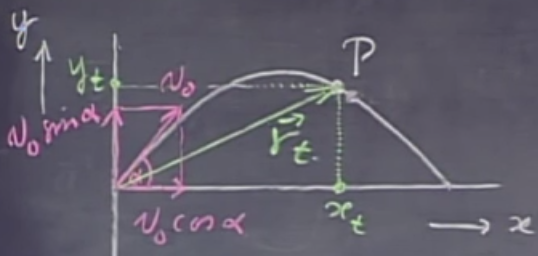
\includegraphics[scale=0.65]{Graphics/2d-motion-decomposed}
\end{center}

The ball moves along the trajectory shown in white. It is launched (thrown) at an initial velocity $v_0$ (in magenta), which is a vector pointing at an angle $\alpha$ from the ground. Also in magenta, we have the initial velocities for the $x$ and $y$ directions, found via vector decomposition:

\begin{align}
v_{0x} &= v_0 \cos \alpha\\
v_{0y} &= v_0 \sin \alpha
\end{align}

Because there is no force acting on the ball in the $x$ direction, this is the velocity it will have in the $x$ direction until it hits the ground.\\
In green, the ball's position vector at a later point is shown, together with its $x$ and $y$ components, all three dependent on time $t$.

We can now apply the equations we found earlier, for one-dimensional motion under either constant acceleration or constant velocity. That is, these:

\begin{align}
x(t) &= x_0 + v_{0x} t + \frac{1}{2} a_x t^2\\
v_x(t) &= v_{0x} + a_x t
\end{align}

The same equations can of course be used for $y$ (and $z$) by simply replacing all $x$ terms with $y$ (or $z$).

With these equations in mind, we can now calculate the object's $x$ position at any moment in time as

\begin{equation}
x(t) = (v_0 \cos \alpha) t
\end{equation}

... since we are free to choose $x_0 = 0$, and there is no acceleration in the $x$ direction ($a_x = 0$).

This simple equation describes the $x$ position completely, from $t=0$ when it is launched, to whenever it hits the ground. To find out when that is, we need to calculate the $y$ position over time.

We use the same equations, with $y_0 = 0$	 (again, we are free to choose where we place our zero coordinate), and $a_y = -g$, that is, the gravitational acceleration of the Earth. $g$ is always positive, however, and in the diagram, we have chosen increasing $y$ to be upwards. Therefore we need to be careful and write $-g$ in this case, or we would be saying that gravity would accelerate the ball towards the sky!

We make the substitutions for the values ($y_0$ and $a_y$ as mentioned above, and the initial velocity in the $y$ direction is $v_0 \sin \alpha$ as we saw before)

\begin{align}
y(t) &= (v_0 \sin \alpha) t - \frac{1}{2} g t^2\\
v_y(t) &= v_0 \sin \alpha - g t
\end{align}

Note the minus sign for the acceleration.\\
The last three equations completely describe the ball's $x$ position, $y$ position, and $y$ velocity. The $x$ velocity is known to be constant.

Together, we can use the $x(t)$ and $y(t)$ equations to describe the trajectory:

\begin{align*}
x(t) &= (v_0 \cos \alpha) t\\
y(t) &= (v_0 \sin \alpha) t - \frac{1}{2} g t^2
\end{align*}

This is then demonstrated in lecture, by firing a golf ball straight up (as seen by the launcher), from a cart moving on a rail.\\
For an outside observer, such as us, the ball moves in a parabolic trajectory, and returns to the launcher a few seconds later, as they moved together at the constant $x$ velocity.\\
The successful demonstration concludes this lecture.

\chapter{Week 2}

\section{Lecture 4: The motion of projectiles}

This lecture doesn't really contain anything new, and instead mostly consists of applications of the material covered last week.\\
Let's revisit this trajectory:

\begin{center}
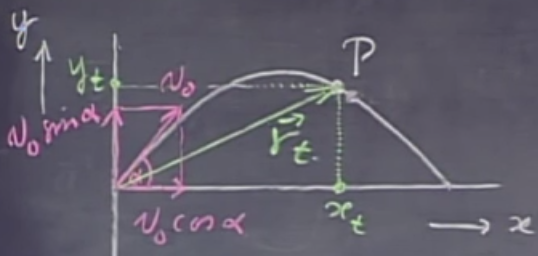
\includegraphics[scale=0.65]{Graphics/2d-motion-decomposed}
\end{center}

For now, ignore the green parts, which are the location of the position vector after a certain time has passed.
Relevant equations for this trajectory can be written as

\begin{align}
x(t) &= (v_0 \cos \alpha) t \label{eq:lec3_x}\\
v_x(t) &= v_0 \cos \alpha\\
y(t) &= (v_0 \sin \alpha) t - \frac{1}{2} g t^2 \label{eq:lec3_y}\\
v_y(t) &= v_0 \sin \alpha - g t
\end{align}

where $v_0$ is the initial velocity diagonally, at angle $\alpha$ to the ground, and $g = +\SI{9.8}{m/s^2}$. Since $g$ is a positive number, we need to use a minus sign here: we have defined increasing $y$ to be upwards, but gravity accelerates downwards.\\
The first and third equations could have $x_0$ and $y_0$ terms, respectively, but we can choose the origin of our coordinate system to be the exact point from where the ball is thrown, which means we choose them both to equal zero.

We can write equation \eqref{eq:lec3_y} above in terms of $x$, instead of $t$, by solving \eqref{eq:lec3_x} for $t$ and making the substitution:

\begin{align}
x(t) &= (v_0 \cos \alpha) t\\
t &= \frac{x(t)}{v_0 \cos \alpha}
\end{align}

\begin{align}
y(t) &= (v_0 \sin \alpha) t - \frac{1}{2} g t^2\\
y(t) &= (v_0 \sin \alpha) \left(\frac{x(t)}{v_0 \cos \alpha}\right) - \frac{1}{2} g \left(\frac{x(t)}{v_0 \cos \alpha}\right)^2\\
     &= x(t) \tan \alpha - \frac{1}{2} g \frac{x(t)^2}{v_0^2 \cos^2 \alpha}
\end{align}

We can then see than this has the form of $x$ times a constant, minus $x^2$ times another constant.

\begin{equation}
y(t) = C_1 x - C_2 x^2
\end{equation}

In other words, the trajectory has the shape of a parabola.

We can calculate when the object reaches the maximum height (the apex of the trajectory), by setting the $v_y(t)$ equation equal to zero. The object is launched with an initial velocity, and will only ever stand ``still'' (on the $y$ axis) when it changes from going upwards to going downwards, since the equation doesn't capture what happens when it hits the ground, etc.

\begin{align}
v_0 \sin \alpha - g t_p = 0\\
g t_p = v_0 \sin \alpha\\
t_p = \frac{v_0 \sin \alpha}{g}
\end{align}

In other words, the time to reach the peak height is simply the initial velocity in the $y$ direction, divided by the acceleration that opposes that motion.\\
We can then find the highest point $h$ that it ever reaches, by substituting the time found above into the $y(t)$ equation:

\begin{align}
h &= (v_0 \sin \alpha) \frac{v_0 \sin \alpha}{g} - \frac{1}{2} g \left(\frac{v_0 \sin \alpha}{g}\right)^2\\
h &= \frac{v_0^2 \sin^2 \alpha}{g} - \frac{v_0^2 \sin^2 \alpha}{2g}\\
h &= \frac{v_0^2 \sin^2 \alpha}{g} \left(1 - \frac{1}{2}\right)\\
h &= \frac{(v_0 \sin \alpha)^2}{2g}
\end{align}

Next up: at what time does the object return to $y = 0$? We could simply set up that equation, solve it, and pick the larger solution (since it will be true at $t = 0$ as well), but we can do it a bit faster. Because the curve is symmetric, the time must be exactly twice that to reach the curve's apex at $t_p$. (The lecture labels the points O at the origin, P at the peak and S where the object lands, but the illustration I used doesn't have them written down.)

\begin{align}
t_s = 2 t_p\\
t_s = \frac{2 v_0 \sin \alpha}{g}
\end{align}

Finally, we can calculate the distance OS, which is the horizontal distance traveled. (Not the entire distance of the parabola, i.e. the arc length!)\\
This distance is simply $v_{0x}$ times $t_s$, but that expression is slightly hairy. Let's write it down and then simplify it:

\begin{align}
\text{OS} = (v_0 \cos \alpha) \left(\frac{2 v_0 \sin \alpha}{g} \right)\\
\text{OS} = \frac{2 v_0^2 \sin \alpha \cos \alpha}{g}
\end{align}

$2 \sin \alpha \cos \alpha = \sin 2 \alpha$ via a trigonometric identity, so:

\begin{align}
\text{OS} = \frac{v_0^2 \sin 2\alpha}{g} \label{eq:lec3_os}
\end{align}

If we want to maximize the horizontal distance, what angle should we fire it at? Well, we could use calculus and attempt to maximize the function, but it can be done much faster (and easier) by simply looking at the equation. $\sin \alpha$ is maximized when $\alpha = \ang{90}$, so $\sin 2\alpha$ must be maximized when $2\alpha = \ang{90}$ or $\alpha = \ang{45}$.

I would not call that immediately obvious, but it is obvious that the answer must be somewhere between 0 and 90 degrees, excluding both of those extremes. At 90 degrees, OS is zero, since the entire trajectory will be one-dimensional in $y$.\\
It cannot be 0 degrees, either, because in that case, it hits the ground instantly after it is fired, so OS is again zero! It's fired completely parallel to the ground, so that $y$ never goes above 0 -- but gravity starts pulling it downwards instantly.\\
The angle must be somewhere between 0 and 90 degrees, and as it turns out, it's exactly in between.

\subsection{Trajectory demonstrations}

We will now try to validate these results in real life, by firing a small projectile (a small metal pellet) at various angles, recording the horizontal distance travelled -- keeping the uncertainties in mind.

First, we measure the maximum height that the pellet can be fired to, a few times. We make an estimate of the height, with an uncertainty, and can use that together with $g$ to calculate $v_o^2$. That is then used in the equation for OS as shown above, to calculate where the pellet should land.

The measurement, along with many others the professor did in preparation, showed the height to be approximately $h_{max} = \SI{3.07(15)}{m}$, so the error is about 5\%.\\
We can solve for $v_0^2$:

\begin{align}
h &= \frac{(v_0 \sin \alpha)^2}{2g}\\
h &= \frac{v_0^2 \sin^2 \alpha}{2g}\\
v_0^2 &= \frac{2gh}{\sin^2 \alpha}
\end{align}

With the value of $h_{max}$ and the error, we find $v_0^2 = \SI{60.2 \pm 3}{m^2/s^2}$. A strange unit, but this is the value we need, rather than $v_0$ itself.

Next, we need to set the angle. There will be uncertainty here, as well -- the professor assumes $\pm \ang{1}$ in his ability to set it up. Since the answer depends on the sine of twice the angle, we may be off by about 2 degrees. However, $\sin{\ang{88}} \approx \sin{\ang{90}}$: the error is about 0.06\%, which pales in comparison to the 5\% error above, so we can completely ignore this source of uncertainty.

Now, using equation \eqref{eq:lec3_os} for OS, we can calculate the predicted horizontal travel distance:

\begin{equation}
\ang{45}\text{ OS} = \frac{\SI{60.2}{m^2/s^2} \sin \ang{90}}{\SI{9.81}{m/s^2}} = \SI{6.14(31)}{m}
\end{equation}

The pellet is fired, and it indeed hits inside the uncertainty range, by the looks of it at more or less 6.05 meters.

Next up, we want to do the same, but at a 30 degree angle, instead. This time, the uncertainty due to the sine of the angle is no longer negligible. What previously was a 0.06\% error suddenly becomes about a 2\% error -- the sine function is roughly ``flat'' around 90 degrees, but far from it around 60 degrees ($2 \times \ang{30}$).

Making the same calculation as we did above, but with the different angle, we find $5.31$ m, but with an uncertainty of 7\% (using an easy  but perhaps not 100\% correct way of calculating uncertainties). That gives us a prediction of $\SI{5.31(37)}{m}$ for the 30 degree angle.\\
Not only did the pellet hit within the uncertainty range, but it actually hit the indicator at the 5.31 meter mark!

Next up: 60 degrees. It turns out that the horizontal distance travelled should be exactly equal to that at 30 degrees, because $\sin({2\cdot\ang{30}}) = \sin({2\cdot\ang{60}})$. $v_0^2$ and $g$ certainly didn't change, so this should indeed be true.\\
The pellet yet again lands within the uncertainty range, though fairly close to being short. This is likely more indicative of the pellet gun's uncertainty and the exact angle than anything else, however -- but it's important to keep in mind that while it was close, it still was \emph{within} the uncertainty. This was certainly no failure.

\subsection{A story about a monkey}

No monkeys were hurt in the making of this demonstration!

Imagine a monkey, sitting in a tree. A short bit away, a hunter places a golf ball cannon, aimed directly at the monkey (dotted line, below).

\begin{center}
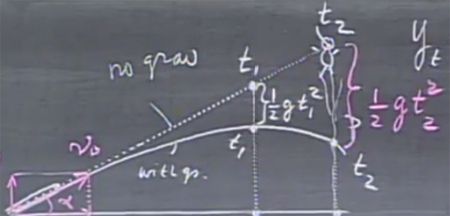
\includegraphics[scale=0.8]{Graphics/lec4_monkey}
\end{center}

We already know that unless the golf ball's velocity is very high, gravity will pull it down in a parabola such that it misses the monkey. Only if the vertical distance travelled due to gravity is smaller than the height of the monkey can it hit.\\
Because the horizontal velocity is the same regardless of whether there is gravity, we know that at a certain time $t$, the golf ball will be at the same $x$ position regardless; only the height will differ.

The dotted line above shows how the ball would travel in the absence of gravity, while the filled line shows the parabolic trajectory it would take on Earth. As we can see, it falls a distance of $\frac{1}{2} g t_1^2$ during a time interval $t_1$ after being fired -- basic 1D kinematics.

However, that is true at all times $t$ after $t = 0$, assuming it has not yet hit the ground (or anything else, for that matter).

Now, there's an additional crux in this problem: as soon as the monkey sees the cannon fire, he lets go and starts falling. The monkey will fall with exactly the same acceleration as the golf ball, and since they started falling at the same time, the golf ball will hit the poor monkey despite his attempt to flee. Had he instead stayed where he was, all would probably be well!

Note that this fact is independent of the golf ball's velocity, as long as it doesn't hit the ground before reaching the monkey's $x$ coordinate. High velocity or low velocity, the gravitational acceleration is the same regardless, and so the ball and the monkey will both fall the same vertical distance in a given amount of time.

Now, let's imagine that all of this happens inside an elevator, which is in free fall. Both the gun and the monkey (and the tree) accelerate downwards at $-g$.

\begin{center}
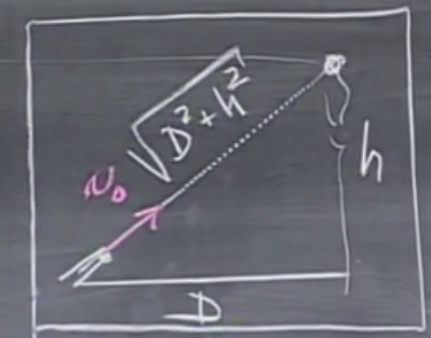
\includegraphics[scale=0.6]{Graphics/lec4_elevator}
\end{center}

From the monkey's point of view, because he falls at the same acceleration and velocity as the gun, the golf ball comes straight at him, without any arcing. As shown above, as far as the monkey can see, the distance the ball has to travel is $\sqrt{D^2 + h^2}$, the hyponenuse of the triangle created by the horizontal distance to the cannon and the (vertical) height of the tree.

Considering the golf ball's velocity, from this point of view, the monkey will get hit in

\begin{equation}
t_{kill} = \frac{\sqrt{D^2 + h^2}}{v_0}
\end{equation}

seconds. However, from a different perspective (see the previous image above), we would instead calculate it as

\begin{equation}
t_{kill} = \frac{D}{v_0 \cos \alpha}
\end{equation}

since $v_0 \cos \alpha$ is the ball's velocity in the horizontal direction.\\
How come the two are not the same? Surely they must both agree? And they do. We can use the definition of $\cos \alpha$ in the above diagram:

\begin{equation}
\cos \alpha = \frac{D}{\sqrt{D^2 + h^2}}
\end{equation}

... and substitute that into what we had just above:

\begin{equation}
t_{kill} = \frac{D}{v_0 \frac{D}{\sqrt{D^2 + h^2}}} = \frac{\sqrt{D^2 + h^2}}{v_0} 
\end{equation}

and so the two agree on the timing of the monkey's unfortunate demise.

\newpage

\section{Lecture 5: Uniform circular motion}

Consider an object moving at a constant speed $v$ around a circle of radius $r$:

\begin{center}
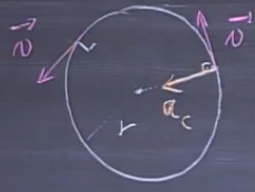
\includegraphics[scale=0.6]{Graphics/lec5_centripetal_acceleration}
\end{center}

We can define a few variables that relate to this motion. First out is $T$, the \emph{period} in seconds it takes the object to travel along the entire circumference once. Second is the \emph{frequency} $f$, which measures how many times it travels around the circle per second. The two are then inverses, so that $f = 1/T$ and $T = 1/f$.\\
The SI unit for frequency is Hertz; the dimension is then $\text{dim Hertz} = \displaystyle \frac{1}{[T]}$, and $\SI{1}{Hertz} = \SI{1}{s^{-1}}$.

We can consider how fast it moves in a different way, in measuring velocity in \emph{radians per second}, instead of meters per second (or other units of ``regular'' velocity). We call this \emph{angular velocity}, symbol $\omega$ (Greek letter lowercase omega). Since there are $2\pi$ radians in a circumference, this implies that

\begin{equation}
\omega = \frac{2 \pi}{T}
\end{equation}

As for the speed $v$ (not the velocity $\vec{v}$ just yet), we can write

\begin{equation}
v = \frac{2 \pi r}{T} = \omega r
\end{equation}

considering the relation shown in the previous equation. These two last equations are important to remember.

\subsection{Centripetal acceleration}

Note that as the object moves around in a circle, the direction of the velocity vector in constantly changing. This can only happen if there is a nonzero acceleration. This acceleration is called the \emph{centripetal acceleration}, often denoted by $\vec{a_c}$. This acceleration vector always points towards the center of the motion. Because the velocity vector is always tangent to the circle at any given point, the acceleration vector is always perpendicular to the velocity, assuming a constant \emph{speed} around the circle. (If the speed is \emph{not} constant, there will also be a tangential acceleration component, which means the net acceleration vector will not be exactly perpendicular to the velocity vector; the centripetal acceleration by itself is however always perpendicular to the velocity vector.)

The magnitude of the centripetal acceleration can be stated as

\begin{equation}
|a_c| = \frac{v^2}{r} = \omega^2 r
\end{equation}

\subsubsection{Proportionality of $r$}
Be careful when it comes to the proportionality of $r$, though! If $T$ is held constant, $v$ is a function of $r$, being equal to

\begin{equation}
v = \frac{2 \pi r}{T}
\end{equation}

and so increasing $r$ will also increase $v$, and thus in the end increase $a_c$:

\begin{equation}
|a_c| = \frac{v^2}{r} = \frac{4 \pi^2 r^2}{r T^2} = \frac{4 \pi^2 r}{T^2}
\end{equation}

Here, it's obvious that increasing $r$ will increase $a_c$, assuming $T$ is held constant. This should come as no surprise, as we are increasing our speed $v$ by moving a longer distance in the same amount of time.

However, let's not fool ourselves into believing that $a_c \propto r$ is always a correct view! Let's now look at the case where we hold the velocity constant (thus changing T) while changing the radius. To get a nice look of how this works, we use the simple equation

\begin{equation}
|a_c| = \frac{v^2}{r}
\end{equation}

Here, holding $v$ constant, it's clear that the centripetal acceleration goes \emph{down} as we increase the radius of the circle we travel in.

\subsubsection{The cause of acceleration}

Something must be causing this acceleration, however. We will introduce \emph{force} next lexture, but for this lecture, we will talk about ``push'' and ``pull'' instead. Suppose you sat on a chair bolted onto a spinning disk. You would feel a ``push'' from the back of the chair, pushing you towards the center of the disk. If you instead tied a rope to a stick at the center, or just held on to a bolted-down stick in front of you, you would feel the rope/stick pulling you inwards. Note that in either case, the pull or push is towards the center.

If the pull/push was suddenly removed somehow, the object would simply continue forward in a straight line, along its velocity vector, unless there are other forces (pushes/pulls) acting on it, such as gravity. This is demonstrated by a spinning disk with a ball tied to a string. The string is cut as the ball's velocity vector points straight upward, and the ball flies several meters straight up in the air, and then falls straight down again.\\
Had it been cut at a different location, it would have followed a parabolic trajectory, as we have studied previously, with $v_0 = v$ and horizontal and vertical components being found by multiplying $v_0$ with the cosine and the sine, respectively, of the angle made with the ground.

\subsection{Planetary orbits}

Let's now have a quick look at the orbits of planets. We will look at them much closer in a few weeks, but until then, let's assume (incorrectly) that orbits are circular. (In reality, they are slightly elliptical.)\\
First out, we have a lecture question:

``The radius of Earth's orbit is $150 \times 10^6$ km. Assuming that the orbit is circular, what is the centripetal acceleration of the Earth?''

They want the answer in $\text{km/yr}^2$, so we shouldn't have to do any ugly conversions.\\
Let's see. The period is one year, by definition (not exactly 365.00 days, but that's another story).

Because $\omega = \frac{2\pi}{T}$ and $T = 1$ year, we find $\omega^2 = 4\pi^2$ radians per year, and $\omega^2 r = (4 \pi^2)(\num{150e6}) = \SI{5.92e9}{km/yr^2}$.

Just to make sure, let's also calculate it using $v^2/r$.

$v$ is found by dividing the circumference of the orbit by the time (1 year), which in then equal in value (but obviously not units) to just the circumference. We then square that, and divide by the radius again; a bit redundant to divide out the radius, but let's go with it for simplicity:

\begin{equation}
v = \frac{2 \pi r}{T} = \frac{2 \pi r}{1 \text{ year}}
\end{equation}

\begin{equation}
a_c = \frac{v^2}{r} = \frac{4 \pi^2 r^2}{r} = 4 \pi^2 r = \SI{5.92e9}{km/yr^2}
\end{equation}

Unsurprisingly, we get the same answer. Still, we have now double-checked, and have also gained a bit of practice doing in two different ways.

Now, let's have a look at the orbits of various planets -- their mean distance to the sun (mean, since the orbits are not truly circular) and periods, and let's compare the centripetal acceleration of various planets. What we find can be seen on this plot below:

\begin{center}
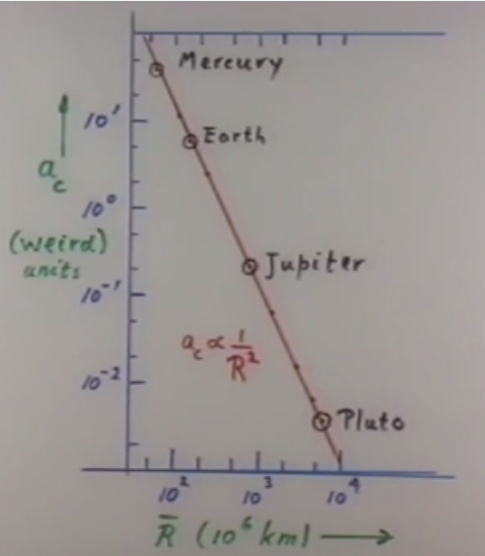
\includegraphics[scale=0.5]{Graphics/lec5_gravity_inverse_r2}
\end{center}

(It's a bit fun to note that Pluto was still considered a planet when the lecture was recorded! Little has changed in classical mechanics since then, but that one thing certainly has.)

Here, we see the centripetal acceleration on the vertical axis, and the mean distance to the sun on the horizontal. It's clear that the $1/R^2$ fit is rather brilliant! The closer a planet is to the sun, the stronger the centripetal acceleration is, and it falls off following the inverse square law.

We've seen centripetal accerelation being proportional to $r$, and inversely proportional to $r$, but now it's inversely proportional to $r^2$! What gives? We will talk more about gravity and planetary orbits soon later in the course. Admittedly, I'm not sure about the exact answer, but looking up data on planetary orbits, I found that planets with larger $r$ also have smaller $v$; the further out you go, the slower planets move through space, in addition to having a lot more distance to cover.

As with the previous examples of centripetal force, if we simply removed the sun (or somehow else removed its gravitational influence), the planets would simply continue on in straight lines, based on their previous velocity vectors.\\
We will discuss gravity further in the coming weeks, but let's leave it here for now: as the distance to the sun is increased by a factor $x$, the effect of gravity is $x^2$ times less. The same is true for e.g. Earth's gravity too, of course, which is why the gravity is weaker further from the surface. (This is however \emph{not} the reason astronauts experience weightlessness, as gravity is still about 90\% as strong on the space station as it is on the surface. They are instead in constant free-fall around the Earth, which is essentially the meaning of an orbit!)

\subsection{Centrifuges and more on centripetal acceleration}

Let's now look at the rotation of a glass tube, with a marble inside. The glass tube starts out horizontal, with the marble inside it (see the first picture below):

\begin{center}
$\vcenter{\hbox{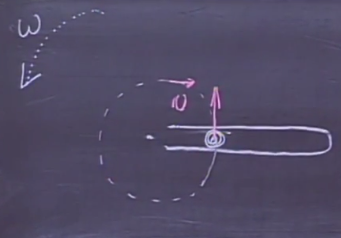
\includegraphics[scale=0.6]{Graphics/lec5_centripetal_acceleration_1}}}$
$\vcenter{\hbox{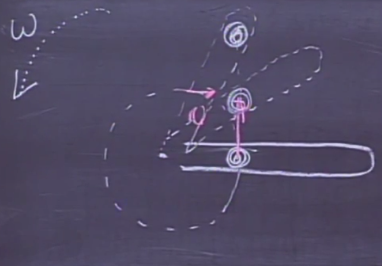
\includegraphics[scale=0.6]{Graphics/lec5_centripetal_acceleration_2}}}$
\end{center}

Because the glass and the marble are both very smooth, the glass can neither push nor pull on the marble, and so cannot provide any centripetal acceleration. What happens? Well, the glass tube will still rotate, of course -- we assume it's powered by a motor of some kind. The marble, on the other hand, will continue on moving according to its still unchanged velocity vector.

A moment later in time (second picture above), the tube has rotated such that the marble's velocity will take it towards the end of the tube, where we know from experience it will also stay, as long as the tube rotates quickly enough.

\subsection{Artificial gravity through centripetral acceleration}

Let's now look at ``perceived gravity'', or artificial gravity.

\begin{center}
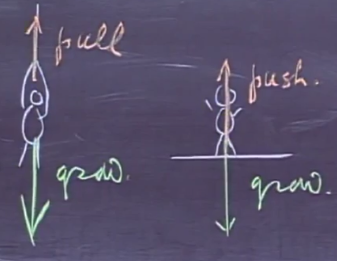
\includegraphics[scale=0.6]{Graphics/lec5_gravity}
\end{center}

As the illustration shows, we will always experience gravity opposite to any pull or push. The same is true if we somehow hang on to a rope and spin around -- or ride a merry-go-round or something to that effect. We will have a centipetral force inwards, and feel a ``pull'' inwards, but perceive gravity in exactly the opposite direction, as if we were drawn outwards.

Let us now consider a large, circular space station, which experiences almost no gravity (as it is in orbit, essentially in perpetual free fall). It is a big ``wheel'', with a radius of 100 m. We want the centripetal acceleration to be about \SI{10}{m/s^2} for a person standing on the outer wall. How fast should it rotate (what should be the period)?

\begin{center}
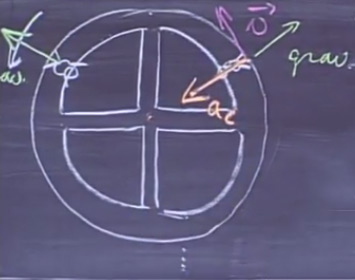
\includegraphics[scale=0.6]{Graphics/lec5_space_station}
\end{center}

We can use $\omega^2 r$ here; it should equal \SI{10}{m/s^2}, so we find

\begin{align}
(\omega^2)(\SI{100}{m}) &= \SI{10}{m/s^2}\\
\omega^2 &= \frac{\SI{10}{m/s^2}}{\SI{100}{m}}\\
\omega^2 &= \SI{0.1}{rad^2/s^2}\\
\omega &= \sqrt{0.1} \text{ rad/s}
\end{align}

And, because $\omega = \frac{2 \pi}{T}$:

\begin{align}
\frac{2 \pi}{T} &= \sqrt{0.1}\\
T &= \frac{2 \pi}{\sqrt{0.1}} \approx \SI{20}{s}
\end{align}

So if we rotated the space station with a period of about/just over 20 seconds, we would perceive it as if we had Earth's gravity.

Now consider how the station might be arranged. The centripetal force is proportional to the distance to the center, so it is strongest at the outer wall. In the exact center of the station, there will be no perceived gravity at all. How does one get there, though? Considering the fact that gravity is perceived as being radially outwards, walking to the center is the same concept as walking to the ceiling in a regular house. You will simply need stairs, ladders, or something similar.

For the same reason, you would have to use the stairs when going back ``down'' as well! The gravitational acceleration may be zero at the center, but it grows as you come closer to the outer edge. If you were to ``jump'' down the shaft, you would end up crashing into the outer wall at a velocity great enough that you may well be killed!

\subsection{More on centrifuges}

Let's have another look at centrifuges.\\
Say we have a liquid filled with very tiny and very light particles; tiny and light enough that they don't sink to the bottom.

\begin{center}
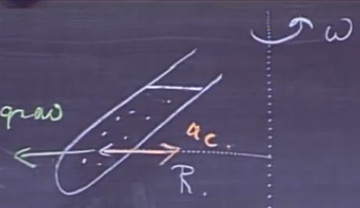
\includegraphics[scale=0.6]{Graphics/lec5_centrifuge}
\end{center}

When we spin it around at a high speed, causing a high centripetal acceleration, the light particles are not so light any longer (as we will soon see, weight is the product of mass and acceleration, the latter of which just incresed by a lot), and they sink to the bottom -- where the centripetal acceleration is the greatest.

Let's make a quick calculation based on a lecture question:

``The frequency of a centrifuge is 60 Hz and its radius is 0.15 m. What is the centripetal acceleration of an object in the centrifuge at a distance of 0.15 m from the center?''

60 Hz is 3600 rpm, so it's spinning rather quickly. We can once again use $\omega^2 r$:

\begin{equation}
|a_c| = \omega^2 r = (2 \pi (\SI{60}{Hz}))^2 \times \SI{0.15}{m} = 21318.3 \approx \SI{21e3}{m/s^2}
\end{equation}

That's over 2000 \emph{times} the acceleration due to gravity, so the particles now experience such an acceleration that they weigh over 2000 times as much as they do in regular gravity!

This is then put to the test in a demonstration. A solution of silver nitrate and sodium chloride is mixed, to produce a milky-white liquid of (most importantly) suspended silver chloride. A part of the solution is put in the centrifuge mentioned above, with a counterbalance of water on the opposite side, to provide stability.\\
The centrifuge is started, and we temporarily move on to other type of centrifuge.

Say we have a bucket of water attached to a rope. We swing it around such that it will be upside down at the top of its motion, with a velocity high enough that $|a_c| > g$. In other words, the bucket experiences an inwards pull due to the centripetal acceleration, which translates into it experiencing gravity in the opposite direction, outwards.\\
Therefore, if we spin it fast enough, the water will be forced into the bottom of the bucket, even when upside down, and no water will come out.

How fast do we have to swing it, if the rope is 1 meter long? (The question also states that the water's mass is 4 kg, which we didn't need to know to solve the problem.)

\begin{align}
\frac{v^2}{\SI{1}{m}} > \SI{9.8}{m/s^2}\\
v^2 > \SI{9.8}{m^2/s^2}\\
v > \sqrt{9.8} \text{ m/s}
\end{align}

We need to swing it faster than about 3.13 meters per second, or the water will start falling.\\
Quickly returning to the silver chloride centrifuge, everything worked out as planned: the liquid is now clear, and there is a collection of white particles at the bottom of the tube, rather than spread out everywhere.

Finally, the water bucket swing is put into practice, and it indeed works.

\section{Lecture 6: Newton's first, second, and third laws}

In this lecture, we will introduce the concept of \emph{force}, an extremely important quantity in physics. Last lecture used forces, but referred to them as ``pushes'' or ``pulls''. We will now start using the correct terminology.

\subsection{Newton's first law}

Newton's first law essentially dates back to Galileo Galilei, in his ``law of inertia''.\\
Newton wrote it as

\begin{quote}
Every body perserveres in its state of rest, or uniform motion in a right line, unless it is compelled to change that state by forces impressed upon it.
\end{quote}

We have seen this in effect already, when decomposing 2D motion: the motion along the horizontal axis has thus far had a constant velocity, since we have ignoring air drag, which acts as a force to slow the object down. Along the vertical axis, on the other hand, we've always had gravity accelerating things downward.

Newton's first law, however, is not valid in all reference frames. It is only valid in inertial references frames, the definition of which is a reference frame where the motion of a particle not under any forces moves in a straight line at constant speed. In particular, this is not true in a reference frame which is being accelerated in any way.

So the question is: can we find an intertial reference frame? Is the lecture hall an inertial reference frame, for example?\\
In can't be. The Earth spins, causing a certripetal acceleration. That's an acceleration, so the answer is already no. There are many additional reasons, though: the Earth moves around the Sun, again causing centripetal acceleration. The Sun moves around the galaxy's center, the galaxy itself has an orbit, and so on.

The Earth has, as mentioned, a centripetal acceleration. We can estimate it by calculating $\omega^2 R_{earth}$, which turns out to be about \SI{0.034}{m/s^2}, which is of course much, much lower than the acceleration due to gravity. If the Earth spun much, much faster, the centripetal acceleration might start to cancel out gravity noticeably, however.

Let's then calculate the centripetal acceleration due to the orbit around the Sun. The radius of the orbit is about $\SI{150e9}{m}$, and the period is of course one year.

\begin{align}
\omega &= \frac{2 \pi}{T} = \frac{2 \pi}{365 \cdot 24 \cdot 60 \cdot 60} = \SI{1.992e-7}{rad/s}\\
a_c = \omega^2 r &= (\SI{1.992e-7}{rad/s})^2 \times \SI{150e9}{m} = \SI{5.95e-3}{m/s^2}
\end{align}

Because the centripetal accelerations calculated above are so tiny, we can consider the Earth as being very close to an inertial reference frame.

A mathematical statement of Newton's first law might be

\begin{equation}
\sum \vec{F} = 0 \Rightarrow \frac{d\vec{v}}{dt} = 0 \text{ (Newton's first law)} \label{eq:newton1}
\end{equation}

\subsection{Newton's second law}

Say we have a spring (though the law isn't specific to springs), in the absence of gravity. We extend the spring, and attach a mass $m_1$ at the end of the spring.

\begin{center}
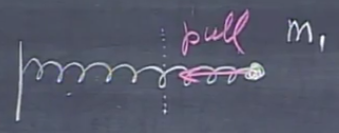
\includegraphics[scale=0.6]{Graphics/lec6_newton2}
\end{center}

Immediately after we let go of the mass, so that the spring's ``pull'' contracts the spring and pulls the mass with it, we measure the acceleration of the mass to be $a_1$.\\
We then replace the mass with another mass $m_2$, and measure the acceleration, in the same manner, to be $a_2$.

We will then find that $m_1 a_1 = m_2 a_2$. The product $m a$ is the \emph{force} (which we have called a ``push'' or a ``pull'' until now) exerted upon the mass by the spring. The spring's force is independent on the mass, but the acceleration caused on the mass is not; the acceleration is inversely proportional to the mass.

In equation form, Newton's second law -- one of the most important equations in physics -- reads

\begin{equation}
\vec{F} = m \vec{a} \text{ (Newton's second law)} \label{eq:newton2}
\end{equation}

As shown above, force is a vector. The direction of the acceleration caused by a force is always in the same direction as the force.

There are other ways of stating it, such as the force being equal to the rate of change of momentum, but we have not yet introduced momentum and so will forget about that for now.\\
The SI unit for force is the newton, in honor of Newton himself, of course. Because the product $m a$ is in units of $\displaystyle \text{kg} \cdot \frac{\text{m}}{\text{s}^2}$, 1 newton equals 1 $\displaystyle \text{kg} \cdot \frac{\text{m}}{\text{s}^2}$.

Just as with the first law, we cannot truly prove Newton's second law. Like the first, it is only valid in inertial reference frames, and we cannot provide such a reference frame to conduct our experiments in.

Note that no statement is made regarding speed or velocity, only acceleration. The law holds equally well at 0 m/s, 5 m/s and 5000 m/s. However, once speeds start becoming noteworthy in relation to the speed of light, Newtonian mechanics becomes more and more inaccurate, and we instead need to use Einstein's relativity for accurate results. This tends to not be an issue in daily life, however, as the two agree very closely at speeds far lower than the speed of light. Even for speeds of 10000 kilometers per second, Newton's equations work quite well (to within about 0.1\%). For speeds below 1000 km/s, in other words all everyday speeds, there is practically no difference at all.

\subsection{Newton's third law}

Let's now have a look at the gravitational force. Using the second law, we see that the force is equal to $m \vec{g}$. Double the mass, double the force, etc.\\
We assume that the lecture hall is an inertial reference frame. Consider an object that is at rest (relative to the lecture hall). We know from the above that there must be a gravitational force on the object, pulling it downwards. However, it is at rest, so there is no acceleration (in our reference frame). Therefore, the net force on it \emph{must} be zero. This is only possible, of course, if there is an equal and opposite force -- or sums of forces that adds up to exactly cancel the gravitational force out.

The above is the result of the third law, which can be stated as

\begin{quote}
If one object exerts a force on another, the other exerts the same force in the opposite direction on the one.
\end{quote}

In other words, if gravity pulls you down into your chair with a force of, say, 700 N, then the chair exerts a force of 700 N back on you. It can be stated more simply as $\text{action} = -\text{reaction}$.\\
We can therefore also write the law as

\begin{equation}
\vec{F_{12}} = -\vec{F_{21}} \text{ (Newton's third law)} \label{eq:newton3}
\end{equation}

where $\vec{F_{ab}}$ means the force exerted \emph{by} object a \emph{on} object b. Note that some physics textbook authors use the reverse notation, which can get confusing.

Unlike the first and second laws, the third laws always holds, including in accelerated reference frames.

Also unlike the first law, there are many intuitive examples of the third:

\begin{itemize*}
\item A garden hose left on its own, with the water on, will start moving backwards. The hose sprays out water by a force, and so the water pushes back on the hose with a force of equal magnitude, and the hose moves backwards.
\item You blow up a balloon, and then let it go. The balloon pushes the air out, so the air pushes on the balloon with an equal but opposite force, propelling the balloon backwards.
\item When you fire a gun, the gun exerts a force on the bullet, and the bullet exerts a force back on the gun: recoil, causing the gun to move backwards unless held steadily.
\item Even when you \emph{walk}, you exert a backwards force on the Earth, which then exerts a force back on you, propelling you forward.
\end{itemize*}

\subsection{Examples of Newton's laws in use}

Let's look at a few examples of Newton's law in practice.

\begin{center}
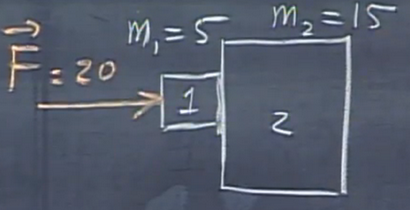
\includegraphics[scale=0.6]{Graphics/lec6_newton3_force}
\end{center}

There's a force of 20 newtons towards the right, as shown. Because the total mass is 20 kg, and the force is 20 newton, there will be an acceleration of $\SI{1}{m/s^2}$ via $\displaystyle \vec{a} = \frac{\vec{F}}{m}$ -- Newton's second law. If not else, we know from intuition and daily life that both objects will move towards the right together, with the same acceleration (and thus velocity, since they started together), once they start moving.

The entirety of the force is on object 1. Since they move together, there must be a force between object 1 and object 2 ($\vec{F_{12}}$), towards the right, or object two could not accelerate.

Since we know that the force on object 1 from the left is 20 N, and we also know that $m_1 = \SI{5}{kg}$ and $a_1 = \SI{1}{m/s^2}$ to the right, we can use Newton's second law to find the net force on object 1 to be 5 N towards the right, despite the force on it from the left being 20 N.

How come? Well, the answer lies in object 2. We know that $m_2 = \SI{15}{kg}$ and $a_2 = \SI{1}{m/s^2}$, so the net force on object 2 \emph{must} be 15 N towards the right. The \emph{only} force on object 2 is $\vec{F_{12}}$, so that too must be 15 N towards the right.

What about object 1? Well, Because of $\vec{F_{12}}$ being 15 N to the right, there must be a force $\vec{F_{21}}$ of 15 N towards the left, back on object 1, which ``cancels out'' most of the 20 N, and leaves object 1 with a net 5 N force to the right. In math form:

\begin{equation}
\vec{F_1} = \vec{F} + \vec{F_{21}} = +20\hat{x} + (-15\hat{x}) = +5 \hat{x}
\end{equation}

... defining the increasing direction of $x$ being towards the right.

Now, what about the sum of forces on object 2? Don't we have 15 N towards the right from object 1, and 15 N towards the left back to object 1, for a net zero force? No! The fact that $a \neq 0$ is enough to prove that this cannot be the case.

It's important to note and understand that the two forces $\vec{F_{12}}$ and $\vec{F_{21}}$ act on different bodies. They don't cancel each other out on an individual object. $\vec{F_{21}}$ is a force that object 2 exerts on object 1 -- that fact does \emph{not} in any way negate the force exerted by 1 on 2! If that were the case, object 2 could not accelerate, since its net force would be zero.

Newton's third law has an interesting, if immeasurable effect: not only do things we drop fall to the Earth, but the Earth always falls towards the things, as well. If we drop an apple from a certain height, there will be a gravitational force on the apple due to the Earth, causing a downward acceleration. However, the third law states that there must be an equal but opposite force on the Earth, due to the apple! The reason we never notice is that the Earth's mass is so extremely large, that the acceleration is on the order of $10^{-24} \text{ m/s}^2$ (or slightly less) or so in the case of an apple, with a total distance moved smaller than $10^{-23}$ m, even for an apple falling from 100 meters above the Earth's surface.\\
Such tiny movements and accelerations are impossible to measure, but they should occur.


\subsection{Newton's laws: summary}

Let's summarize Newton's laws, and point out a few possible pitfalls.

\textbf{Newton's first law} states that a body with no external forces (or no \emph{net} external force) on it will remain as it is, either at rest or moving at constant velocity in a straight line. This only holds true in inertial reference frames! If you are in a car, moving at a \emph{constant velocity} past a street lamp, from your (inertial) frame of reference, the street lamp moves with constant velocity -- and there certainly shouldn't be any net force on it, so all is well.\\
If you accelerate, however, you will see the street lamp appear to accelerate without any net force on it. This is because your car is no longer an inertial reference frame, since it is accelerating with respect to the reference frame of the Earth (and the lamp), so the first law does not hold.

\textbf{Newton's second law} states (in one form) that the acceleration of a body is equal to the \emph{net} force on that body, divided by the body's mass. The acceleration vector is in the same direction as the force vector.\\
Mass is a measure of inertia, i.e. how much a body resists changes in motion. The larger the mass, the smaller the acceleration, for a given magnitude of force.

\textbf{Newton's third law} states that whenever an object $a$ exerts a force on a body $b$ (an ``action force''), there is an equal but opposite force (a ``reaction force'') exerted by object $b$ back an $a$.\\
This implies that when you are pulled downwards by the Earth, you also pull the Earth upwards.\\
However, it does \emph{NOT} imply that when you sit on a chair, and the Earth pulls you down, the chair pushes you up! This is a \emph{very} important distinction. An action-reaction pair \emph{always} acts on different bodies, but note that the gravitational force and the chair's force both act on you!\\
The \emph{second} law implies that if you don't move, the chair\footnote{Or something else, or a combination of things, such that the net force is zero.} must push you back up with a force of equal magnitude but opposite direction, because the net force on you must be zero if your acceleration is zero.

\textbf{Another possible pitfall} is to say that force is the cause of motion -- not true! Force is the cause of \emph{change} in motion, that is, acceleration. You can travel at any velocity with no forces on you whatsoever -- in fact, the first law tells us that.\\
On a related note, keep in mind that while in daily speech, acceleration refers to increasing your speed, while in physics, acceleration simply means change in speed. You accelerate when stopping your car -- the acceleration is in the opposite direction of the velocity (and will thus be negative if the velocity is positive), but it's an acceleration nonetheless.

\textbf{Finally, the kilogram is a unit of \emph{mass}, not of weight}. In daily speech, the two are the same, but in physics, they are distinct quantities, and it's very important to understand how they differ and how they are related.

\emph{Mass} is the measure of how difficult it is to change the motion of an object. Whether we think about pushing something to get it moving, or to try to stop something from moving does not matter: both will become more difficult as mass increases.\\
The mass of an object is independent of where it is located; it is a property of an object due to its makeup.

\emph{Weight}, on the other hand, is the force exerted on an object by gravity. You can calculate your approximate weight on Earth as $m g$, where $g = \SI{9.8}{m/s^2}$ is the approximate gravitational acceleration at the Earth's surface.\\
The weight of an object \emph{changes} based on the local gravitational force -- a person weighs much less on the Moon than they do on Earth, but their mass would be the same in either location.

A scale measures weight, not mass, but usually converts the measurement to a mass by dividing the measured force by $g$, which then via Newton's second law yields the mass.\\
This means that if you bring a regular bathroom scale to the Moon, and weigh yourself on it, it will report about 1/6 of your actual mass, as the force of gravity is so much smaller on the Moon, but the scale doesn't know that it has moved: it will still divide the measured weight in newtons by \SI{9.8}{m/s^2}, and find an incorrect answer. The weight it \emph{measures} is correct, but the mass it reports is not.

\subsection{Tension and another example of Newton's laws in use}

Say we hang a mass $m$ from two strings, suspended at different heights. The leftmost string makes an angle of 45 degrees with the roof above, while the rightmost string makes an angle of 60 degrees. We call the tension in the rightmost string $T_1$, and in the leftmost $T_2$. We consider increasing $x$ to be towards the right, and increasing $y$ to be upwards.

\begin{center}
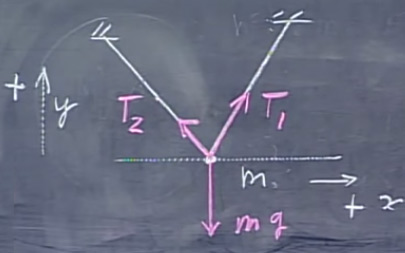
\includegraphics[scale=0.6]{Graphics/lec6_tension}
\end{center}

There will be a gravitational force of magnitude $m g$ downwards. Because the object is in equilibrium, sitting still with no acceleration, the \emph{net force} on the object must be zero -- that is clear from Newton's second law.\\
Therefore, we conclude that the two tensions $T_1$ and $T_2$ perfectly balance the gravitational force $m g$, so that the net force on the object is zero.

Force is a vector, so we can decompose this into two one-dimensional problems. We don't need to decompose the gravitational force, of course: it is already only in the $-y$ direction. Let's decompose the tension vectors, though.

Let's start with $T_1$. It makes a 60 degree angle with the horizontal, so by using vector decomposition, we find

\begin{align}
T_{1x} &= T_1 \cos(\ang{60}) = \frac{T_1}{2}\\
T_{1y} &= T_1 \sin(\ang{60}) = \frac{T_1 \sqrt{3}}{2}
\end{align}

As for $T_2$, it makes a 45 degree angle, so the sine and cosine are both one over the square root of two. (It makes sense that the force is equal in both directions, since the angle is exactly in the middle of a 90 degree angle, so to speak.)

\begin{align}
T_{2x} &= T_2 \cos(\ang{45}) = \frac{T_2}{\sqrt{2}}\\
T_{2y} &= T_2 \sin(\ang{45}) = \frac{T_2}{\sqrt{2}}
\end{align}

What then? Well, we know that the net force must be zero, since there is no acceleration. The same can be said for each axis independently, too: $\sum F_x = 0$ and $\sum F_y = 0$. We can set up equations representing this:

\begin{align}
T_{1x} + T_{2x} = 0\\
\frac{T_1}{2} - \frac{T_2}{\sqrt{2}} = 0\\
T_1 = \frac{2 T_2}{\sqrt{2}} = \sqrt{2} \cdot T_2 \label{eq:lec6_t1}
\end{align}

Note that because $T_2$ points towards the negative $x$ direction, the sum of these two forces becomes a subtraction.

As for the $y$ axis:

\begin{align}
T_{1y} + T_{2y} = m g\\
\frac{T_1 \sqrt{3}}{2} + \frac{T_2}{\sqrt{2}} = m g\\
T_2 = \sqrt{2}\left(m g - \frac{T_1 \sqrt{3}}{2}\right)
\end{align}

Alternatively, we could have written $T_{1y} + T_{2y} - m g = 0$ (minus $m g$ since it is in the opposite direction) to show that the sum is zero, rather than saying that they must be equal. This is of course the same thing algebraically.

We now have two equations with two unknowns. Let's substitute the value of $T_1$ into the second equation from \eqref{eq:lec6_t1} and find $T_2$ as a function of only $m$ and constants:

\begin{align}
T_2 = \sqrt{2}\left(m g - \frac{\sqrt{2} T_2 \sqrt{3}}{2}\right)\\
T_2 = \sqrt{2} m g - T_2 \sqrt{3}\\
T_2 + \sqrt{3} T_2 = \sqrt{2} m g\\
T_2 (1 + \sqrt{3}) = \sqrt{2} m g\\
T_2 = \frac{\sqrt{2} m g}{1 + \sqrt{3}}
\end{align}

Since $T_1 = \sqrt{2} T_2$, $T_1$ is simply

\begin{equation}
T_1 = \frac{2 m g}{1 + \sqrt{3}}
\end{equation}

We can finally substitute in some values. The lecture used $m = \SI{4}{kg}$, so let's try that. We find

\begin{align}
T_1 &= \frac{(2)(\SI{4}{kg})(\SI{9.8}{m/s^2})}{1 + \sqrt{3}} \approx \SI{28.7}{N}\\
T_2 &= \frac{T_1}{\sqrt{2}} \approx \SI{20.3}{N}
\end{align}

The professor's answers differ slightly, but match up perfectly if we use $g = \SI{10}{m/s^2}$, so he most likely used that approximation.

As a sanity check, and additional practice, let's just make sure that the forces indeed balance out.

\begin{align}
T_1 \cos(\ang{60}) - T_2 \cos(\ang{45}) &\overset{?}{=} 0\\
14.35 - 14.35 &= 0
\end{align}

... so that indeed works out in the $x$ direction. Let's check $y$:

\begin{align}
T_1 \sin(\ang{60}) + T_2 \sin(\ang{45}) &\overset{?}{=} m g\\
24.85 + 14.35 &= 39.2
\end{align}

It works out perfectly!

\chapter{Week 3}

\section{Lecture 7: Weight, perceived gravity, and weightlessness}

This lecture will discuss weight, its relation to mass, and other related topics.

A regular scale, say a bathroom scale, measures weight -- which is a \emph{force}. Therefore, it measures in newtons, if we stick to SI units. We can only use a scale to find \emph{mass} in kilograms by knowing the local gravitational acceleration, and dividing that out of the measured result.

As a result of this, such a bathroom scale would measure a mass only 1/6 as great on the moon, where the local gravitational acceleration is about 1/6 of Earth's. This is because the \emph{weight} of the object being weighed has decreased, since the gravitational force is weaker. However, the \emph{mass} of the object has not changed. If the scale made the calculation using the local gravitational acceleration, the measured/calculated mass would be correct. Most don't, of course, and assume the Earth's gravitational acceleration of about $g \approx \SI{9.8}{m/s^2}$, and so display a much too small value for the mass when they divide the smaller weight by the incorrect gravitational acceleration, which is only valid on Earth's surface.

In other words, if the scale displayed weight in newtons, it would display the correct value everywhere, only that the correct value would differ based on location. The person's mass would not change with location, however, so a scale that is used to measure mass should always display the same value for a particular person.

So, you stand on a bathroom scale. Gravity is acting on you to pull you downwards, and as you are not being accelerated, there must be a net force on zero on you. Therefore, we conclude that the scale is pushing you up, with a force of the same magnitude, $F_{S} = m $g. This force that the scale exerts on you is the definition of your \emph{weight}.

Now, we move the scale and you into an elevator.

\begin{center}
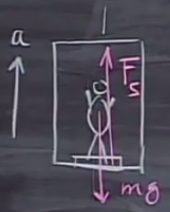
\includegraphics[scale=0.8]{Graphics/lec7_elevator}
\end{center}

Again, gravity acts on you with a force $m g$ downwards. The scale pushes back up with force $F_S$. However, now, the elevator is being accelerated upwards. The net force must now be positive (upwards), not zero, since you could not have a nonzero acceleration with zero net force.

We find that $F_S - m g = m a$, so $F_S = m(a + g)$. The reading of the scale has increased, and increases linearly with increasing acceleration upwards. If the elevator accelerates upwards at $2g \approx \SI{20}{m/s^2}$, your weight would be three times as high as usual. Only when $a_y = 0$ is your measured weight as it usually is.

Let's now reverse the situation. We now consider increasing $a$ to be downwards, and the elevator is now accelerating downwards. In other words, $a > 0$.

Again, you have gravity acting downwards with a magnitude $m g$. If that were the only force, you would be in free fall with acceleration $g$, so there must be some upwards acting force. On the other hand, $|m g| > |F_S|$ or there would be no acceleration at all, so while $|F_S|$ is smaller than the force gravity exerts on you, it's still there.

Back to Newton's second law.

\begin{equation}
m g - F_S = m a
\end{equation}

Reading that out loud, it does make a lot of sense: if $F_S = m g$, then $m a$ is zero, and we are not accelerating. If $m g$ is dominant, we are accelecating downwards (since $a > 0$ means downwards acceleration).

Rearranged,

\begin{equation}
F_S = m(g - a)
\end{equation}

The larger the downwards acceleration, the \emph{less} you weigh. I think most of us have experienced this (and the reverse situation) in fast elevators (that accelerate quickly).

Now, imagine we cut the cable of the elevator. What happens? Well, our equation has the answer. The net acceleration $a$ will be equal to the acceleration from gravity $g$, so $F_S = 0$. That is, the scale will show you to have zero weight -- and you will, because you are now in free fall. You are falling downwards, but other than that, you wouldn't notice gravity the same way we do now. The things falling with you wouldn't care about up or down -- a glass filled with water would act the same whether upside down or not.

This is very similar to how things work in the space shuttle and on the International Space Station (ISS). Their orbits around the Earth keep them in constant free fall, only they never hit the surface, as they are going sideways with great velocity (about 7.7 km/s!). We will talk much more about orbits later in the course.

In short, weightlessness is when the forces acting on you are exclusively gravitational. You're not being held up by any floors, ropes, seats, etc, just falling due to gravity pulling on you.

Let's now look at another type of scale:

\begin{center}
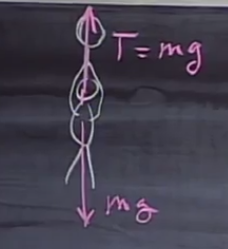
\includegraphics[scale=0.8]{Graphics/lec7_hanging}
\end{center}

The scale in this case is a tension meter, inside the string we are hanging from. Because we are hanging still, not accelerating, the tension in the string must equal the force of gravity pulling us down. Therefore, the tension meter reads $m g$, same as it would on a regular scale standing on the floor.\\
Thus we see that it makes no difference whether we measure the force a scale is pushing us up with, or the force a rope/tension meter \emph{pulls} us up with.

Let's now accelerate this system. We accelerate it upwards, which must mean the tension in the string goes up -- it must be greater in magnitude than $m g$ or we wouldn't accelerate upwards.\\
Just as with the elevator, we find $T - m g = m a$ or $T = m(a + g)$. Same as before, only we use $T$ for tension instead of $F_S$ for force exerted by the scale.\\
If we instead accelerate downwards, we again find the same result as before, as do we if we simply cut the string and go into free fall.

Say we have the following system:

\begin{center}
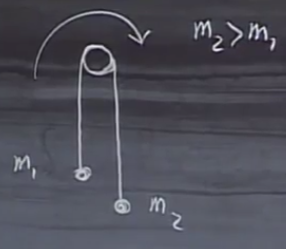
\includegraphics[scale=0.8]{Graphics/lec7_pulley}
\end{center}

The string is massless, the pin/pulley is massless, but the two objects hanging an each end are not; the right one at mass $m_2$ has a greater mass than that of $m_1$ to the left.

What happens? Well, we know from intuition and experience that the system will accelerate as shown. $m_2$ will fall down, while $m_1$ will be pulled up.

Because we consider the case where there is no friction, and the string is massless, the tension in the left side must equal the tension on the right side. Only in the case of no friction and a massless string is this true, however.

Why is that, though? It's relatively easy to show. Consider a small piece of the string on the left side. It has gravity pulling the mass $m_1$ down, and a force upwards because of the mass $m_2$ on the other side of the pulley. If the two forces were not equivalent, the massless string would experience an acceleration $a = \frac{F}{0}$ -- that's clearly impossible.	

The same argument can be used for any part (of any length) of the string. The tension must be equal everywhere.\\
Again, this is only true because we consider the string massless, and the pulley frictionless.

Now, we earlier showed that the tension in the string is an indicator of the weight hanging from it. That means that while this acceleration is taking place, $m_1$ and $m_2$ have the same weight! The obviously don't have the same \emph{mass}; that's different, by definition of $m_2 > m_1$. Because weight is mass times acceleration, however, the \emph{weight} of $m_1$ has increased, as it is being accelerated upwards (think about the elevator and the bathroom scale), while the weight of $m_2$ has \emph{decreased}, since it is acceleratin downwards (falling, though not in free fall, so it still has a weight larger than zero).

Let's calculate the acceleration and tension for these objects and strings.\\
$m_1$ accelerates upwards. The tension in the string is $T = m_1 g$ while it is in equilibrium, but that cannot be the case now. The force upwards must be greater than $m g$, or it cannot accelerate upwards. Therefore, the tension in the string must be the sum of the downwards force due to gravity, plus the extra ``perceived'' gravity from the upwards acceleration. In total, we have $T = m_1 a + m_1 g = m_1(a + g)$.

For the second object, gravity pulls downwards with force $m_2 g$, while the string tension pulls back up. This object is accelerating downwards, however, so $m_2 g$ must be greater in magnitude than the tension. However, remember that the tension must be the same as in the case of the first mass! It's the same string, and as we showed earlier, we get an impossible situation if the tension differs throughout the string.

To avoid sign confusion, we now denote \emph{downwards} acceleration to be positive. We write the tension out as an equation, and find $T = m_2 (g - a)$.

We now have two equations, so we can set them equal and solve for the acceleration $a$:

\begin{align}
T = m_1(a + g)\\
T = m_2(g - a)\\
m_1 a + m_1 g = m_2 g - m_2 a\\
m_1 a + m_2 a = m_2 g - m_1 g\\
a(m_1 + m_2) = g(m_2 - m_1)\\
a = \frac{g(m_2 - m_1)}{m_1 + m_2}\\
\end{align}

We can then substitute that value into $T - m_1 g = m_1 a$ that we found earlier:

\begin{align}
T - m_1 g = m_1  \frac{g(m_2 - m_1)}{m_1 + m_2}\\
T = \frac{2 g m_1 m_2}{m_1 + m_2}
\end{align}

The algebra isn't shown, but this is indeed the case.\\
These two results make intuitive sense. If we set $m_1 = m_2 = m$, we find $T = m g$ and $a = 0$. All is as it should: the tension on a string with a weight $m$ hanging from it better be $m g$, if it's not accelerating! Likewise, $a$ better be zero, since both masses and weights are equal, so there is no net force on either mass.

If we even consider as $m_2 \to 0$, we find that the tension goes to zero, and the acceleration goes to $g$ (in magnitude). This is because $m_1$ is now in free fall, and since $m_2$ is massless and the string is massless, there is nothing left to cause tension in the string. The acceleration is $-g$ since it is simply in free fall -- nothing is holding it up.

We can also show that if $m_2 > m_1$, then the relationship $m_1 g < T < m_2 g$ will hold for this system. As they are being accelerated, the tension will be equal for both masses. Therefore, $m_1$ must gain weight, and $m_2$ must lose weight. (Keep in mind that $m_1$ accelerates upwards, so it gains weight, like in an elevator, and $m_2$ accelerates downwards, and so it loses weight.)

\subsection{Weightlessness}

We talked a bit about perceived gravity and so on last week. Let's expand on it.

Consider the case where we are swinging an object around a rope of length $R$ in the vertical plane. $R$ is then the radius of the circle the object traces out.\\
Gravity with force $m g$ acts downwards at all times. We spin the object with angular velocity $\omega$.

The string will have a tension $T$, which will change in direction as the thing spins, of course. The magnitude should also change -- if the angular velocity is low, just on the edge of this working out, the tension should be zero at the top. Any slower, and the string will slack off and the object starts falling down.

Let's calculate the tension. First, we know there will be a centripetal acceleration $|a_c| = \omega^2 R$. That must be the case, or the object cannot travel around in a circle like this, period.

At the lowest point of the circle, gravity acts downwards with force $m g$, while the tension upwards is $T$. There's also the centripetal force $m a_c$. We have not really used the term centripetal force yet, but it's a force, so it's found by the centripetal acceleration times the mass in question.

All in all, we find $T - mg = m a_c$, so that $T = m(a_c + g)$. This equation looks almost exactly like the one for acceleration in an elevator, which we found earlier. If $a_c = g$, you tension of the string would be twice the weight of the object.

Now, let's look at the top of the circle instead. As we did earlier, we will now reverse out sign convention so that downwards forces and accelerations are positive.\\
As before, the tension and the force of gravity add up to the centripetal accerelation, so we find $T + m g = m a_c$, so that $T = m(a_c - g)$.

This is just about exactly the same equation as we had for the elevator accelerating downwards, losing weight.\\
If $a_c = g$, the tension will be zero, and the object will be weightless. If $a_c > g$, there will be tension in the string, equal to the object's weight.\\
$a_c$ cannot be smaller than $g$, however. That would give us negative tension, which can't happen. What this implies is that this situation simply would never happen: if $a_c < g$, then the object would never reach the top while tracing out a circle, but would have started falling prior to reaching the top.

The rest of the lecture is mostly demonstrations and related talk, which I didn't find it very useful to take notes for, but it's certainly worth watching, of course.\\
One thing is worth writing down though. The lecture talks about parabolic plane flights -- they start by upwards at a $\approx 45$ degree angle, then follow a parabolic trajectory (free fall) with the engines off, and then re-start the engines and repeat.

This causes the plane to be in free fall for about 30 seconds at a time, during which time any traveller would experience weightlessness -- but \emph{not zero gravity}. There are absolutely similarities between free fall and zero gravity (which you could almost experience far, far from any planets or stars, but certaintly not on Earth), but they are not the same.

Zero gravity implies that the Earth's gravity somehow stops acting on the people in the plane, despite the fact that Earth's gravity is almost as strong up there as it is at the surface. Even at the ISS, in orbit at an altitude of about 350 km (which is quite close to the surface for a ``space'' station, all things considered), the gravitational pull is about 90\% of the strength it is near the surface.\\
The astronauts are then weightless for exactly the same reason: they are constantly falling ``towards'' the Earth, only they have such a huge sideways velocity, that they never hit it.

We will talk more about gravity later in the course, including how $g$ is calculated etc.

\section{Lecture 8: Frictional forces}

Let's talk about friction. Thus far, we have ignored friction (and air drag) in all problems we've solved; that will now start to change.

Let's look at a simple case to begin with. We have an object at rest, on a flat surface:

\begin{center}
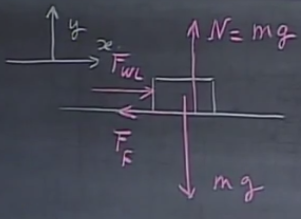
\includegraphics[scale=0.8]{Graphics/lec8_friction}
\end{center}

There is a gravitational force of magnitude $m g$ pulling the object down, and a \emph{normal force} $N = m g$ (also in magnitude) from the surface on the object, or it could not be at rest; Newton's second law. (Again, however, note that this is NOT a case of Newton's third law; there two forces both act on the object, and so they are not an action-reaction pair.)

We (the professor) exerts a force $F_{WL}$ (WL for Walter Lewin) in the $+x$ direction. Because of friction, the object will not start to move unless the force is great enough. (Without friction, any force, no matter how small, causes an acceleration, even if it's tiny.)

There is a frictional force $F_F$ in the $-x$ direction that exactly cancels out the force we apply. We push harder and harder, and eventually the frictional force reaches its maximum value, at which point we overcome it and the object starts to accelerate.

It is then experimental fact that this maximum, $F_{Fmax}$, is

\begin{equation}
F_{Fmax} = \mu N
\end{equation}

where $\mu$ is a friction coefficient.\\
We can differentiate between the \emph{static} friction coefficient $\mu_s$ and the \emph{kinetic} (or dynamic) friction coefficient $\mu_k$.

$\mu_s N$ is the frictional force we need to overcome to get a resting object to start moving, while $\mu_k N$ is the force we need to overcome to keep it moving.\\
We know from experience that it takes more force to get something to move in the first place, so $\mu_s > \mu_k$ -- ``always'', the lecture says, but there does appear to be some strange exception to this rule. I'm assuming this course will not cover (or mention) them, however.

We can calculate a friction coefficient by putting an object on an incline, and measure the angle of incline required to get the object to move (due to the gravitational force downwards, of course).

\begin{center}
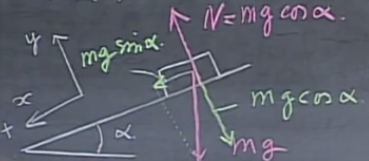
\includegraphics[scale=0.8]{Graphics/lec8_friction_incline}
\end{center}

Note the choice of coordinate system, which is tilted such that the acceleration (and movement) in the $y$ direction will always be zero, but more importantly such that the $y$ axis is exactly perpendicular to the surface of the incline.\\
The downside to this approach is then that we need to decompose the gravitational force, since it is no longer strictly in one axis.

Because of how the angle $\alpha$ is defined, the strength of the gravitational force in the $y$ direction is $m g \cos \alpha$ (if $\alpha = 0$, $\cos \alpha = 1$ and so it is strictly in the $y$ direction), while that in the $x$ direction is $m g \sin \alpha$. This is a bit opposite to how it usually is ($x$ tends to use the cosine, while $y$ uses the sine), but it should make sense why this is.

There is a normal force $N$ opposing $m g \cos \theta$, which must be equal in magnitude -- there is no acceleration in the $y$ direction, so the net force along that axis must be zero, via Newton's second law.

There is a frictional force $F_F$ in the negative $x$ direction, equal in magnitude to $m g \sin \alpha$ (the gravitational force along the slope), since the object is still not moving. We gradually increase the angle, which increases $F_f$, but of course also the gravitational force in the $x$ direction (downwards along the slope). Sooner or later, the frictional force reaches its maximum, and gravity ``wins''.

How do we then calculate $\mu_s$, the static friction coefficient, in terms of the angle $\alpha_{max}$ (the maximum angle possible before the object starts to slide)?

Well, it should be easy! We know the strength of the force pulling the object: $m g \sin (\alpha_{max})$. We know that $F_F = \mu_s m g \sin (\alpha_{max})$ must exactly equal this force in magnitude to keep it standing still.\\
We also know that $F_F = \mu_s N$, as we mentioned earlier.

Therefore, we set the two equal, and we can solve for $\mu_s$. $N = m g \cos \alpha$, so

\begin{align}
\mu_s m g \cos (\alpha_{max}) = m g \sin(\alpha_{max})\\
\mu_s = \frac{m g \sin(\alpha_{max})}{m g \cos (\alpha_{max})}\\
\mu_s = \frac{\sin(\alpha_{max})}{\cos (\alpha_{max})} = \tan(\alpha_{max})
\end{align}

So finding the static friction coefficient is truly simple: measure the maximum angle possible before the object starts to slide, take the tangent of that angle, and you're done! And, since the incline makes a triangle with the vertical height, horivontal length and the incline itself (the hypotenuse), we can measure this even without knowing angles; we can calculate the angle even if we can only measure distances.

Note that two seemingly important quantities are nowhere to be seen in this result: the mass of the object does not matter, and neither does the amount surface area that is in contact with the incline!\\
This means that two parked cars -- a large truck and a small car,will start to slide at the same angle, if they were tilted together, so to speak. Not only does the mass not matter, but the width of the tires (or the amount of tires) also does not matter.

These two facts are then demonstrated qualitatively, by sliding a few objects down a wooden plank. Indeed, adding a few times the mass to a plastic container didn't change the result by much (but by a little -- because the plank is not exactly uniform, the containers may not be identical, etc.). Neither did it make a noticeable difference to slide down two small pieces of wood, one lying down (large contact area) and one standing on the edge (small contact area).

\subsection{Friction on a block with a pulley}

Let's look at a different, but related example. We have the following setup:

\begin{center}
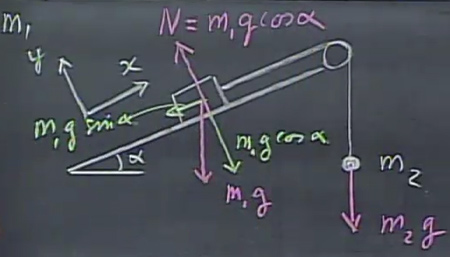
\includegraphics[scale=0.8]{Graphics/lec8_friction_pulley}
\end{center}

A block of mass $m_1$ is sitting on an incline, with the same gravitational force, decomposed as previously.\\
However, this time, a second mass $m_2$ hangs on a massless and fixed-length string (increasing tension doesn't increase the length of the string), over a pulley (which itself is massless and frictionless).

As before, there is no movement of the  block in the $y$ direction, so we be sure that the normal force $N$ must exactly cancel out the gravitational force of $m_1 g \cos \alpha$ in our rotated $-y$ direction.\\
The string has a tension, since mass $m_2$ is hanging on it. As before, since the string is massless and has a fixed length, the tension must be the same everywhere in the string.

Now... This situation has a tricky part that the previous one didn't: depending on the friction coefficient of the block, and the magnitude of masses $m_1$ and $m_2$, one of three things can happen: the block can accelerate ``downhill'', it can accelerate ``uphill'', or it can simply stand still. We need to consider all of these possibilities when solving this problem. Because of this, we do not know in which direction of the frictional force is; we only know that it always opposes the object's motion, which could be either $+x$ or $-x$.

We do know that the maximum magnitude of the frictional force is

\begin{equation}
F_{Fma} = \mu_s N = \mu_s m_1 g \cos \alpha
\end{equation}

The tension in the string, $T$, can be drawn as a vector opposing $m_2 g$, in the string above mass $m_2$.

We will now evaluate three different situations. In all cases, the system is at rest for now, but what is about to happen differs: there's the case where it's \emph{just} about to start accelerating towards the left (downhill for the block), the case where it's \emph{just} about to start accelerating in the other direction, and the case where it will remain at rest/in equilibrium.

Because the system is rest, the tension must be of magnitude $m_2 g$, so that it exactly balances the gravitational force on mass $m_2$, and as mentioned previously, that tension is the same in all parts of the string.

\subsubsection{Case 1: About to accelerate uphill}

We will first look at the case where $m_2$ ``wins'', and the block is \emph{just} about to start moving uphill, but is \emph{still at rest}.\\
In this case, the frictional force is at a maximum $F_{Fmax}$, which opposes the direction it's about to move it, so $F_{Fmax}$ acts together with gravity in the $-x$ direction.\\
We can write Newton's second law for the system:

\begin{equation}
T - m_1 g \sin \alpha - F_{Fmax} = 0\text{ (we substitute $T = m_2  g$)}
\end{equation}
\begin{equation}
m_2 g = m_1 g \sin \alpha + F_{Fmax}
\end{equation}

Tension acts ``uphill', while the other two act ``downhill'', and they must sum to zero since $a$ is still zero.

When this equation is true, the block is \emph{just} about to move uphill. Therefore, we can write a criterion for the uphill motion:

\begin{equation}
m_2 g \ge m_1 g \sin \alpha + F_{Fmax}
\end{equation}

If $m_2$ increases in mass by even the tiniest bit, the system will start to accelerate so that $m_2$ starts moving downwards.

\subsubsection{Case 2: About to accelerate downhill}

In this case, the frictional force is in the same direction as the tension, and thus in the opposite direction of gravity. We write Newton's second law again:

\begin{equation}
T + F_{Fmax} = m_1 g \sin \alpha\\
\end{equation}
\begin{equation}
m_2 g = m_1 g \sin \alpha - F_{Fmax}
\end{equation}

If $m_2$ is just a tiny bit \emph{smaller} (or $m_1$ greater, or $F_{Fmax}$ smaller), the system will start moving downhill. Therefore, the criterion for downhill motion is

\begin{equation}
m_2 g \le m_1 g \sin \alpha - F_{Fmax}
\end{equation}

\subsubsection{Case 3: Neither case matches}

In case neither of the two conditions are met, the system will simply sit in equilibrium. The frictional force will be ``adjusted'' so that it causes the net force in the $x$ direction to equal zero.

\subsubsection{Example case}

Let $m_1 = \SI{1}{kg}$, $m_2 = \SI{2}{kg}$, $\mu_s = 0.5$ and $\mu_k = 0.4$, while using $g = \SI{10}{m/s^2}$ for our calculations, just to get an idea. Also, let $\alpha = \ang{30}$.

What will happen in a system with these parameters? Well, we have three possible cases, with equations (or inequalities) we can look at. Since both conditions depend on the same three force terms, let's calculate their values:

\begin{align}
m_2 g &= \SI{20}{N}\\
m_1 g \sin \alpha &= \SI{5}{N}\\
F_{Fmax} = \mu_s m_1 g \cos \alpha &\approx \SI{4.33}{N}
\end{align}

Let's now look at each of the two conditions. For the block to start sliding uphill, substituting in the values, we must have $\SI{20}{N} \ge \SI{5}{N} + \SI{4.33}{N}$. Since that is true, the block will indeed start sliding uphill. Let's just verify that the second case is false, just for the sake of argument. We need $\SI{20}{N} \le \SI{5}{N} - \SI{4.33}{N}$, which is certainly not the case. So indeed, only one case matches, and it says the block will start accelerating uphill.

Let's now attempt to calculate the magnitude of the acceleration, and the string tension. We know that it will start moving uphill, so the frictional force is then downhill, in the $-x$ direction. The magnitude of this force now changes, however: the block is in motion, and so we must now use the kinetic friction coefficient $\mu_k$ instead. Using that, we find

\begin{equation}
F_{Fmax} = \mu_k m_1 g \cos \alpha
\end{equation}

We can again write Newton's second law for this case. The tension is uphill, gravity downhill, and friction downhill. Those forces must equal $m_1 a$, where $a$ is the uphill acceleration. (Since the block is now being accelerated, the net forces no longer sum to zero.)

\begin{equation}
T - m_1 g \sin \alpha - \mu_k m_1 g \cos \alpha = m_1 a
\end{equation}

We need a second equation, however. $T$ is unknown -- because $m_2$ is now being accelerated downwards, it is ``falling'' or ``losing weight'', so $m_2 g > T$ or the object could not accelerate down!\\
Since $m_2$ will never change, and we are still on Earth's surface, $g$ can also not change. The only thing that \emph{can} change is the tension. The tension \emph{must} go down, or $m_2$ simply cannot accelerate downwards!

The second equation can be found by thinking about mass $m_2$. Because the string has a fixed length, the acceleration of this mass \emph{must} be equal to that of the block sliding uphill. Anything else and clearly, the string would need to get either longer or shorter, depending on which acceleration was greater.

Because they are equal in magnitude, then, we can write a second law equation for mass $m_2$, using positive values for the downwards direction (so that this $a$ has the same positive sign as the other $a$ uphill):

\begin{equation}
m_2 g - T = m_2 a
\end{equation}

Solving this system, we get a fairly complex answer, unless we substitute in the numbers early. If we do, we find $a \approx \SI{3.85}{m/s^2}$ and $T \approx {SI}{12.3}{N}$. If we don't, we find, after simplification,

\begin{equation}
a = g\ \frac{m_2 - m_1 (\mu_k \cos \alpha + \sin \alpha)}{m_1 + m_2}
\end{equation}

And for the tension:

\begin{equation}
T = g m_1 m_2 \frac{1 + \mu_k \cos\alpha + \sin \alpha}{m_1 + m_2}
\end{equation}

Two things are important to note from the numerical results we found. One is that the acceleration was a positive number. We had already calculated that the block should move uphill, and since the positive $x$ direction is uphill, a negative acceleration would mean it should move backwards. We already know that is not the case, so the acceleration must be positive in this case.

Second, the tension must be smaller than $m_2 g$, or that mass couldn't possibly be accelerating downwards. If $m_2 g$ doesn't ``win'' over the tension, how could the mass be accelerating downwards?

Let's take a quick look at what would happen in the same system, if $m_2 = \SI{0.4}{kg}$ instead. In that case, $m_2 g = \SI{4}{N}$. Let's look at the conditions again. Is it true that $\SI{4}{N} \ge \SI{5}{N} + \SI{4.33}{N}$? No, certainly not. Is it then true that $\SI{4}{N} \le \SI{5}{N} - \SI{4.33}{N}$? No, that's not it, either.

Since neither condition is met, the system will stay as it is, with $a = 0$. Note that the equations we derived just above, for $a$ and $T$, are not valid in this case and cannot be used. They only hold in the case of accelerations upwards, since that is what we derived them for.

What will happen is that the frictional force will be adjusted so that together with the tension, it holds the object up.

\chapter{Week 4}

This week had only one lecture, and it was all a review from weeks 1-2, so I only worked through the problems and didn't take any notes.\\
There is one interesting bit at the very end, though, which is worth watching even now that the exam has closed.

\chapter{Week 5}

\section{Lecture 10: Hooke's law, simple harmonic oscillator}

Say we have a spring, in its ``relaxed'' state, i.e. in equilibrium. We choose to place $x = 0$ at the spring's end, and then extend the spring a distance $x$.

There will be a restoring force that attempts to pull the spring back to its original length. For many springs, it is approximately true that this restoring force $F$ is proportional to the displacement $x$.\\
For an \emph{ideal spring}, we can write the force as

\begin{equation}
F = -k x
\end{equation}

where $k$ is known as the spring constant, and the minus sign signifies that the force opposes the displacement. (If $x$ is positive to the right, the force will be to the left, and vice versa.)\\
This also holds if the spring is compressed (shortened) instead of stretched.\\
The above relation is known as \emph{Hooke's law}.

We can measure this spring constant in a few different ways. Perhaps the simplest would be to hang a mass from a spring and measure how far it extends due to the pull of gravity. When it is in equilibrium, we know that the upwards force from the spring must equal the downwards force due to gravity. Therefore, we can measure $x$ and $m$, and we know $g$, so we can calculate the spring constant:

\begin{align}
|F| = k x &= m g\\
k &= \frac{m g}{x}
\end{align}

Assuming we work in SI units, the units of the spring constant must then be in newtons per meter.

If we instead change the masses, we will get a plot that is a straight line, assuming Hooke's law holds. We can then find $k$ as the slope of this line:

\begin{center}
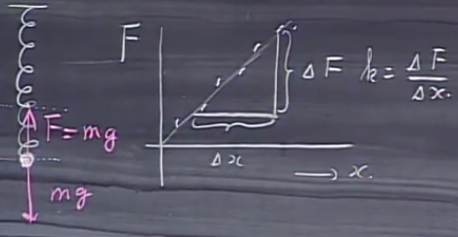
\includegraphics[scale=0.7]{Graphics/lec10_measure}
\end{center}

This is probably a more reliable test than the single calculation above, since it will show if Hooke's law doesn't hold for the particular spring, instead of silently assuming that it does.

Hooke's law has its limitations, as you might expect. It's possible to stretch a spring so far that it permanently changes its shape, in which case the restoring force will not increase linearly, but grow slower than Hooke's law would predict.

Let's look at a second way of measuring the spring constant of a given spring. Say we have another spring, again with $x = 0$ at the end of spring's relaxed length. We extend the spring further, and attach a mass $m$ to the end of the spring. The mass rests on a frictionless surface.

\begin{center}
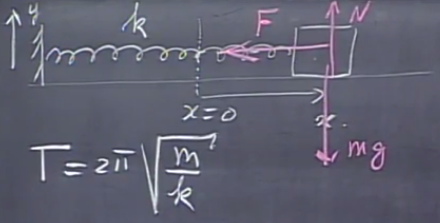
\includegraphics[scale=0.7]{Graphics/lec10_sho}
\end{center}

When we let the mass go, this system will begin to oscillate. The spring force pulls the mass towards the left until it is relaxed, but when that happens, the mass is already moving towards the left, and has inertia in that direction. The spring will be compressed, and now push on the mass, which eventually comes to a halt, accelerates back towards the right, etc.

Because of the relationship shown, which will be derived shortly, we can either calculate a spring constant from a known mass (while using a stopwatch), or me can measure a mass, if we know the spring constant, even in the absence of gravity! Note that there is no relation to $g$ in the formula. The only place where it appears is in the pull of gravity and the normal force, but since the surface is taken to be frictionless, neither force matters for the oscillation period.

It's interesting to note that the amplitude of the oscillation, i.e. how far it moves horizontally from the center point, does not affect the period at all. If the amplitude is small, it will move slowly back and forth, but if the amplitude is large, it will move at much greater speed, to keep the period constant -- assuming Hooke's Law holds.

\subsection{Simple harmonic oscillators: mathematical derivation}

Let's have a look at the situation we have above. We apply Newton's second law to the system, and find

\begin{equation}
m a = - k x
\end{equation}

Written in alternative notation, and divided through by $m$:

\begin{align}
m \ddot{x} + k x = 0\\
\ddot{x} + \frac{k}{m} x = 0
\end{align}

$\dot{x}$ is used to signify the first time derivative of position (velocity), while $\ddot{x}$ is used for the second time derivative (acceleration).

Prof. Lewin calls this last equation ``arguably the most important in all of physics''. It is the equation that governs simple harmonic oscillators; there are many kinds of such oscillators.

First, it is demonstrated that the solution for $x(t)$ should be some form of sinusoid. Trying to keep this as general as possible, we can write

\begin{equation}
x = A \cos(\omega t + \varphi)
\end{equation}

Here, $A$ is the amplitude (how far it swings, from the center point), $\omega$ is the \emph{angular frequency} (not to be confused with angular velocity), in radians/second, and $\varphi$ is the \emph{phase angle}, in radians.

As we have seen many times before,

\begin{equation}
T = \frac{2 \pi}{\omega}
\end{equation}

since if you increase $t$ by $T$ seconds, the argument to the cosine will have increased by $2 \pi$ radians $= \ang{360}$, and the function repeats.

We can write this in terms of frequency (``regular'' frequency in Hertz, i.e. the number times something happens per second, rather than angular frequency):

\begin{equation}
f = \frac{1}{T} = \frac{\omega}{2 \pi}
\end{equation}

(We can think of the last equations as being in radians per second, divided by $2 \pi$ radians; the ``per second'' is then all that remains.)

Next, we substitute our ``trial answer'' into the equation relating $x$ and $\ddot{x}$. To do that, we must first find $\ddot{x}$, i.e. the second derivative of $x$ with respect to time. Keeping in mind the chain rule, we find

\begin{align}
x        &= A \cos(\omega t + \varphi)\\
\dot{x}  &= A \omega (-\sin(\omega t + \varphi) = -A \omega \sin(\omega t + \varphi)\\
\ddot{x} &= -A \omega^2 \cos(\omega t + \varphi)
\end{align}

Now, because $x = A \cos(\omega t + \varphi)$, we can also write

\begin{align}
\ddot{x} = -\omega^2 x
\end{align}

All in all, our differential equation becomes

\begin{equation}
- \omega^2 x + \frac{k}{m} x = 0
\end{equation}

Because this must always hold for all $x$, it must be the case that

\begin{align}
w^2 = \frac{k}{m}\\
\omega = \sqrt{\frac{k}{m}}
\end{align}

With the equation we already had for $T$, it turns out that

\begin{align}
T = 2 \pi \sqrt{\frac{m}{k}}
\end{align}

... as shown in the figure prior to this derivation.

As we can see, the period is inpedendent on the amplitude, and also independent on the phase angle $\varphi$. More on that now.

When we start this oscillation, we can decide two things: how far we stretch the spring before we let the mass go, and how much (if any) of a push we give it, i.e. initial velocity. The amplitude and phase angle will be decided by these \emph{initial conditions}.

Say we give it a push, so that $\vec{v} = -3\hat{x}$ m/s, while it is at $x = 0$ at $t = 0$. With all these conditions, we can find both the amplitude $A$ and the phase angle $\varphi$. We know the equation must hold true at $x = 0$ at $t = 0$, since that's a given, so we plug that in:

\begin{align}
0 = A \cos(\varphi)
\end{align}

This equation can be true in two cases: $A = 0$, or $\cos(\varphi) = 0$. $A$ cannot be 0, because we know there will be an oscillation with a nonzero amplitude. Therefore,

\begin{align}
\cos(\varphi) = 0\\
\varphi = \frac{\pi}{2}, \frac{3\pi}{2}
\end{align}

Either value of $\varphi$ makes the cosine zero. (There are of course an infinite number of such angles, but we restrict them to $0 < \varphi < 2\pi$.)

Since we have a time-varying position, we can take the time derivative to find the velocity as a function of time, and relate that to the initial condition $v = -3$ m/s.

We calculate the time derivative of the equation (which we did earlier), and substitute in the values, including $t = 0$, and set it equal to $-3$ m/s:

\begin{align}
x = A \cos(\omega t + \varphi)\\
\dot{x} = -A \omega \sin(\omega t + \varphi)
\end{align}

Keep in mind that $\dot{x} = v$.\\
In with the values, and solve:

\begin{align}
-3 = -A \omega \sin(\pi/2)\\
-A \omega = -3\\
A = \frac{3}{\omega}
\end{align}

Say the object has a mass $m = \SI{0.1}{kg}$, and the spring has a spring constant of $k = \SI{10}{N/m}$.

We find $\omega$ as

\begin{equation}
\omega = \sqrt{\frac{k}{m}} = 10 \text{ rad/s}
\end{equation}

So $A = 0.3$ meters, and the full equation that explains this oscillation is

\begin{equation}
x(t) = 0.3 \cos(10 t - \frac{\pi}{2})
\end{equation}

\subsection{Motion of a pendulum}

Next up, we have a look at the equations that govern a pendulum's motion.

\begin{center}
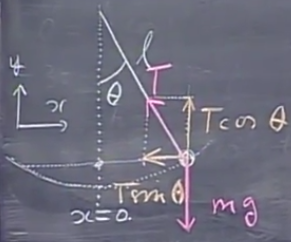
\includegraphics[scale=0.7]{Graphics/lec10_pendulum}
\end{center}

We have a mass $m$ attached to a string of length $\ell$, which is swinging back and forth. We choose a coordinate system with its origin at the pendulum's center, decompose the forces, and write down Newton's second law for the system.

Gravity is pulling downwards on the mass, while there is a tension in the string pulling upwards (but not straight upwards, of course). We decompose this tension, and write down the equation for the $x$ direction:

\begin{equation}
m a_x = m\ddot{x} = - T(\theta) \sin \theta = -T(\theta) \frac{x}{\ell}
\end{equation}

$a$ is towards the right (since that is the positive direction of the coordinate system), but the horizontal component of the tension is towards the left at this moment. The second equality holds for trigonometric reasons.

For the $y$ direction, we find

\begin{equation}
m \ddot{y} = T(\theta) \cos \theta - m g
\end{equation}

We then have two coupled differential equations to solve, which is above this course's level... but we can simplify things a bit.\\
We start out by making some approximations. First out is the small angle approximation, which is usually used to imply that $\sin \theta \approx \theta$ and $\cos \theta \approx 1$ if $\theta \ll 1$ radian (it works quite well up to 0.2 rad $\approx \ang{11.5}$ or so, at least, where $\cos(0.2) \approx 0.98$ and $\sin(0.2) \approx 0.1987$).

There is a second important approximation we can make if we assume the angle will always be small. Have a look at the diagram above, and note how the $x$ amptitude is much greater than the $y$ amplitude. For a 5 degree swing, the $x$ motion is about 25 times as large as the $y$ motion, and it is still 11 times as large at 10 degrees.\\
We can therefore approximate the acceleration in the $y$ direction to be zero, so we find

\begin{align}
0 = T(\theta) - m g\\
T = m g
\end{align}

The cosine disappears, since we approximated it to be one, and the left-hand side disappears since $a = \ddot{x} \approx 0$.

We substitute this into our differential equation for $x$, and find

\begin{align}
m\ddot{x} = -m g \frac{x}{\ell}\\
m\ddot{x} + m g \frac{x}{\ell} = 0\\
\ddot{x} + \frac{g}{\ell} x = 0
\end{align}

Compare this to the spring-mass system, which obeyed $\displaystyle \ddot{x} + \frac{k}{m} x = 0$ -- this is another simple harmonic oscillator!

Since the only difference between the differential equations is, practically, two variable names, the solution is of course the same. We find these equations for this system:

\begin{align}
x = A \cos(\omega t + \varphi)\\
\omega = \sqrt{\frac{g}{\ell}}\\
T = \frac{2 \pi}{\omega} = 2 \pi \sqrt{\frac{\ell}{g}}
\end{align}

Keep in mind that these results are limited to the case where the angles are small, and the string can be considered massless in comparison to the mass at the end of the string.

Now, let's compare the results we found for the spring/mass system and the pendulum on a string.\\
For the oscillating spring, the period depends on the spring constant and the mass $m$. This can be explained simply, as follows: when you extend a spring, there is a restoring force, proportional to the distance you extended it. However, the force is not in any way dependent on the mass of the object you attach to the spring; therefore, the acceleration is inversely proportional to the mass, via Newton's second law:

\begin{align}
|a| = \frac{|F_{spring}|}{m} = \frac{k |x|}{m}
\end{align}

If the acceleration is very low, clearly the period must increase.

As for the pendulum, the period is independent on the mass. Why?\\
Again, this can be shown quite easily. If $m$ doubles, $m g$ doubles, and so the tension $T = m g$ must also double (since the $y$ acceleration is the same -- approximately zero). The restoring force $T \sin \theta$ is proportional to $T$, so that doubles as well. If the mass doubles and the force doubles, the acceleration stays exactly the same, and so the period is not affected.

Next, $k$ and $g$. If $k$ is high, the period is short, which makes sense: the acceleration is proportional to $\sqrt{k}$, so for very large $k$ (meaning a very stiff/strong spring -- remember that it's in newtons per meter of displacement) the acceleration is high, and the period low.\\
As for the pendulum, it is \emph{inversely} proportional to $\sqrt{g}$, so if $g$ is low, the period is very large, and it goes to infinity as $g \to 0$. A pendulum could not work in weightlessness, where the perceived gravity is zero, since it relies on gravity to swing. (This too is easy to see: the restoring force is proportional to $g$, so with $g \approx 0$, there shouldn't be any restoring force, nor any string tension.)

``All'' that remains in the lecture is one of the best demonstrations in this class, which means no notes taken, but careful watching instead!

\section{Lecture 11: Work, energy and universal gravitation}

Let's get started right away.\\
\emph{Work} is a measure of the amount of energy a force uses when moving an object. In simple applications, it can be defined as $W = F d$, where $F$ is the magnitude of the force, and $d$ is the distance the object moves.

A more useful definition, still in one dimension, is an integral, which then can take care of non-constant forces as well:

\begin{equation}
W_{AB} = \int_A^B F\ \mathop{dx}
\end{equation}

... where $A$ and $B$ are the $x$ coordinates where the object starts out, and ends up, respectively.

Work is a scalar quantity, and can be negative, zero or positive.\\
It is positive if the force and the displacement are in the \emph{same} direction, and negative if they are in the \emph{opposite} direction. It can be zero, e.g. if there is no displacement.

The SI unit of work is the joule, J, which from the definition clearly is the same as a force of 1 newton times a displacement of 1 meter. We rarely if ever write Nm for work; though Nm and J are mathematically equivalent, Nm is used for torque (which will be introduced later in the course).

Since $\displaystyle F = m a = m \frac{dv}{dt}$, and distance $dx = v dt$, we can rewrite this integral in terms of velocity:

\begin{equation}
W_{AB} = \int_A^B m \frac{dv}{dt} v \mathop{dt} = \int_{v_A}^{v_B} m\ v \mathop{dv} = \Big[ \frac{1}{2} m v^2 \Big]_{v_A}^{v_B} = \frac{1}{2} m \left(v_B^2 - v_A^2\right)
\end{equation}

Here, we have also found the formula for kinetic energy, often notated as $K_E$, $K_e$ or just $K$:

\begin{equation}
K_E = \frac{1}{2} m v^2
\end{equation}

If an object of mass $m$ is moving at velocity $v$, the above formula can calculate its kinetic energy, i.e. how much energy is required to accelerate it to that velocity.

In other words, using the above two relations, we can see that

\begin{equation}
W_{AB} = \Delta K_E = K_{EB} - K_{EA}
\end{equation}

This is known as the \emph{work-energy theorem}. The difference in kinetic energy of an object is equal to the amount of work done on it by the net forces acting on it.\\
If the kinetic energy has increased when moving from point A to point B, the work is positive; if the kinetic energy has decreased, the work is negative, and if the kinetic energy is unchanged, the net work is zero.\\
Note that it's positive for multiple forces to work against each other, such that one provides positive work, a different force provides negative work, etc. such that the \emph{net} work, and thus the change in kinetic energy, can be either positive, negative or zero, depending on the strengths and angles of the forces.

Let's try an applied example. Say an object is moving upwards, while gravity acts on it downwards as you'd expect.\\
We choose the positive $y$ axis to be upwards, so gravity is $-mg\hat{y}$. The object has a velocity $v_A$ where it starts out at point A, and moves upwards to point B while losing speed due to gravity.

We now want to calculate the distance $h$ between points A and B, assuming that the object comes to (temporary) rest at point B.\\
We apply the work-energy theorem, with $\displaystyle K_{EA} = \frac{1}{2} m v_A^2$ and $K_{EB} = 0$.\\
The gravitational force is constant with a magnitude of $m g$, so the work gravity does is $m g h$. The direction of the force is downward, and the motion is upwards, so the work is negative.\\
We set the two equal and solve for $h$:

\begin{align}
- m g h = 0 - \frac{1}{2} m v_A^2\\
g h = \frac{1}{2} v_A^2\\
h = \frac{v_A^2}{2 g}
\end{align}

We have seen this result before, but we found it in a quite different way last time.

As a second example, say we lift an object against gravity, a height $h$ above where it started out. It starts with 0 speed, and also ends up with 0 speed. Via the work-energy theorem, the net work must be zero, since the object's kinetic energy did not change.\\
Gravity still does its work of $|F h| = |m g h|$, only that it's negative here: the force direction is down, and the motion is up. Since gravity does work $- m g h$ on the object, we, who lift it, must then provide positive work $m g h$ in order to make the net work zero.

If we instead reverse the situation, and lower the object closer to the ground, the opposite thing happens. Gravity does positive work $m g h$, while we provide negative work $- m g h$ when lowering the object, and again the net work must be zero, if the object both starts out and ends up with no kinetic energy.

It's important to realize that work, as used in physics, is far from the same as we might think intuitively.\\
If we lower a very heavy object from a height down to the ground, we will have provided negative work, $- m g h$, but we for sure have still \emph{spent} energy burned in our muscles to provide it. We didn't get some sort of added energy reserve from doing so, even though the work is negative.\\
Likewise, we can get tired from holding an object perfectly still (try holding something heavy at arm's length for an extended period of time!), despite the fact that $F d = 0$ and no work has been done.

\subsection{Taking the step to three dimensions}

We can extend what we have above to three dimensions. Say we apply a force $\vec{F}$ over a path. For each tiny point of this path, we can find a vector $\vec{dr}$, which represents a infinitesimal displacement along the line; so small that we can approximate it as a straight line, rather than some form of curve.

\begin{center}
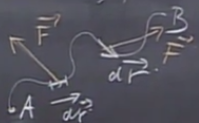
\includegraphics[scale=0.8]{Graphics/lec11_work_3d}
\end{center}

The net work done by the force over the entire path is

\begin{equation}
W_{AB} = \int_A^B = \vec{F} \cdot \vec{dr}
\end{equation}

A dot product integral may look scary, but they're not too bad.\\
By the way, the above is a \emph{line integral} (or \emph{path integral}, or \emph{contour integral}): it evaluates an integral along a path.

We can decompose this integral into three one-dimensional integral -- surprise! -- to make it easier to solve. In general terms, we can write the force vector and the displacement vector as sums of components:

\begin{align}
\vec{F}  &= F_x \hat{x} + F_y \vec{y} + F_z \hat{z}\\
\vec{dr} &= dx \hat{x} + dy \hat{y} + dz \hat{z}
\end{align}

With this in mind, we can find $dW$, a small amount of work done by the force over a small distance $dr$, using the definition of the dot product:

\begin{equation}
dW = \vec{F} \cdot \vec{dr} = F_x \mathop{dx} + F_y \mathop{dy} + F_z \mathop{dz}
\end{equation}

Integrate both sides, and we find

\begin{align}
W_{AB} = \int_A^B \vec{F} \cdot \vec{dr} &= \int_A^B \left(F_x \mathop{dx} + F_y \mathop{dy} + F_z \mathop{dz}\right)\\
                                    &= \int_A^B F_x \mathop{dx} + \int_A^B F_y \mathop{dy} + \int_A^B F_z \mathop{dz}
\end{align}

We now have three one-dimensional problems to solve, instead. Not only that, but we've already solved this integral in one dimension. We just need to add it up for the three dimensions:

\begin{equation}
W_AB = \frac{1}{2} m \left( v_{Bx}^2 - v_{Ax}^2 \right) + \frac{1}{2} m \left( v_{By}^2 - v_{Ay}^2 \right) + \frac{1}{2} m \left( v_{Bz}^2 - v_{Az}^2 \right)
\end{equation}

Not pretty... but that's probably the last time we'll see it written like that. Here it is again, re-arranged, but exactly equal to the above:

\begin{align}
W_AB &= \frac{1}{2} m \left( v_{Bx}^2 + v_{By}^2 + v_{Bz}^2 \right) - \frac{1}{2}m  \left( v_{Ax}^2 + v_{Ay}^2 + v_{Az}^2 \right)\\
     &= \frac{1}{2} m \left( v_B^2 - v_A^2 \right)
\end{align}

... and so we find exactly the same result as we did in one dimension.

Let's as an example calculate the work done by gravity while moving an object around in 3D space.

\begin{center}
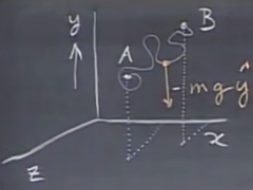
\includegraphics[scale=0.8]{Graphics/lec11_3d_path}
\end{center}

We move from a point $A$ to a point $B$, where $y_B - y_A = h > 0$, in other words, point B is higher up than point A.

The force due to gravity is $- m g \hat{y}$, so the integral would be

\begin{equation}
W_{gravity} = \int_A^B \vec{F} \cdot \vec{dr} = \int_A^B (- m g) \mathop{dy} = - m g \int_A^B \mathop{dy} = -m g(y_B - y_A) = -m g h
\end{equation}

The $x$ and $z$ terms disappear, since $F_x = 0$ and $F_z = 0$ -- gravity only acts along one axis, with the way we've defined our coordinate system.

We find that the work done by gravity is negative, as it should be -- the force vector is down, but the object moved higher up. The net work of the force(s) that moved it upwards, in the $y$ direction, is then $+ m g h$.\\
(We can't say anything about the work along the $x$ and $z$ axes without more information, of course.)

Another thing is interesting about this result: it is independent of the path between points A and B. The only thing that matters, as far as gravity is concerned, is the difference in height. If you move an object up 10 meters and back down 9, the work done by gravity is exactly the same as if you'd just moved it up the one meter. The same goes for all and any movement in the x-z plane, which doesn't affect the work done by gravity whatsoever.

Any force that has the property that the work done is the same for any given pair of start/end points, regardless of the path moved in between them, is called a \emph{conservative force}. As we have just shown, gravity is conservative. If a particle starts at one point, moves around in any path whatsoever, and comes back to that exact point, the work done by gravity is always zero.

\subsection{Conservation of mechanical energy}

We can apply the work-energy theorem to the equation above:

\begin{align}
-m g(y_B - y_A)& = K_{EB} - K_{EA}\\
-m g\ y_B - m g\ y_A &= K_{EB} - K_{EA}\\
K_{EA} + m g\ y_A &= K_{EB} + m g\ y_B
\end{align}

This is a very important result. The quantity $m g y$ is what we call \emph{gravitational potential energy}, often $P_E$ or $U$. What the above result says, then, is that the sum of the kinetic and potential energies at point A must equal the sum of the kinetic and potential energies at point B.

\begin{equation}
K_{EA} + U_A = K_{EB} + U_B
\end{equation}

This is known as the \emph{conservation of mechanical energy}, where the mechanical energy of an object is the sum of its kinetic energy and its potential energy. One can be converted into the other, but \emph{as long as the forces involved are conservative}, the sum of the two must stay equal. This condition is an important one! Friction, for example, is \emph{not} a conservative force, and this relationship will no longer hold if frictional forces are involved.\\
Spring forces \emph{are} conservative, however.

The fact that frictional forces are not conservative should be fairly intuitive. The further we move something against friction, the more total work must be done to overcome the friction. You could move something back and forth on a table and the work done by the friction (and you, in moving it) would just increase and increase in magnitude.\\
If you did the same against gravity, moving something up, then back down, etc., the work done (by gravity, or by you) would \emph{not} simply increase without bound.

With the definition of $K_E = \frac{1}{2} m v^2$, it's clear that kinetic energy is zero when the velocity $v$ of an object is zero.\\
What about potential energy? That is zero where $y = 0$, but where is that? It is up to us to decide where to place that point. We are free to choose it, as long as $g$ is the same at both point $A$ and point $B$ (or simply that $g$ is close enough, so that we can neglect the difference).

\subsubsection{Example problem}

\begin{center}
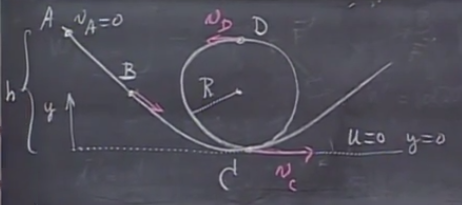
\includegraphics[scale=0.8]{Graphics/lec11_conservation}
\end{center}

We place an object on this ``roller coaster'', at point A, which is $h$ above the line where we choose $y = 0$ and $U = 0$. It gains speed, by converting gravitational potential energy to kinetic energy, until it reaches point C, where the velocity (and the kinetic energy) is at a maximum, while the potential energy is zero, by our definition.

At that point, it reaches the loop. The question is: from what height $h$ must we let it go along the track, so that it manages to move around the loop without falling out before reaching the top?

We can apply the conservation of mechanical energy to this problem, assuming friction is negligible:

\begin{equation}
U_A + K_{EA} = U_B + K_{EB} = U_C + K_{EC} = U_D + K_{ED}
\end{equation}

We let it go from rest at point A, so $K_{EA} = 0$. Our definition of potential energy as $U = m g h$, where $h$ is the height above the plane where $U = 0$.\\
The vertical distance is must travel ``upward'' in going around the circle is twice the radius, so $2R$.

If we equate the total mechanical energy at A, $U_A = m g h$, with the total mechanical energy at any given point, we can find

\begin{align}
m g h &= m g y + \frac{1}{2} m v^2\\
v^2   &= 2g (h - y)
\end{align}

This equation should hold for any point, again assuming we can neglect friction and other forces. At point D, at the top of the loop, the constraint that $a_c > g$ must hold, or we know that it will fall out of the loop, instead of being pushed against it by the centripetal force.

Since centripetal acceleration is given by $\displaystyle a_c = \frac{v^2}{r}$, and we know $v^2$, we can write an inequality for this being larger than $g$, and then solve for $h$, to find the answer to our question about the minimum height we must release the object from.\\
$y = 2 R$ at this point, so

\begin{align}
\frac{2g (h - 2R)}{R} &\ge g\\
2 h - 4R &\ge R\\
2 h &\ge 5R\\
h &\ge \frac{5}{2} R
\end{align}

So if we find a point along the roller coaster where this condition is met, and perhaps add a small amount due to friction, the ball will ``make the loop'', so to speak. Without friction, air resistance etc., it would come up to the exact same height as it started rolling down from.

\subsection{Newton's law of universal gravitation}

Like the previous laws we've learned with Newton's name attached to them, the law of universal gravitational is quite simple.

Say we have two masses, often named $m$ and $M$ (where it's often the case that $M$ e.g. a planet, and $m$ is smaller; this is of course no requirement, however). The two point masses\footnote{This also works for masses of nonzero size in some cases, more on that at a later time.} are separated by a distance $r$. The force that $m$ experiences because of $M$ is then

\begin{equation}
F = \frac{G M m}{r^2}
\end{equation}

in the direction of $M$ (gravity is always an attractive force), where $G$ is the gravitational constant, not to be confused with $\displaystyle g \approx \frac{G M_{Earth}}{R_{Earth}^2}$ (approximately because Earth's mass is not all at the center; Earth is not a perfect sphere, etc.).\\
$G$ has a value of about $6.67 \cdot 10^{-11}$, with units that need to cancel out with the others, i.e.

\begin{align}
\text{[N]} = \frac{\text{[G]} \text{[kg]}^2}{\text{[meter]}^2}\\
\frac{\text{[N]} \text{[meter]}^2}{\text{[kg]}^2} = \text{[G]}
\end{align}

So in more terse notation, the units of $G$ are $\text{N} \cdot \text{m}^2 \text{kg}^{-2}$.

Because of $F = ma$, so $\displaystyle a = \frac{F}{m}$, we can find the gravitational acceleration due to a mass $M$ to be the force, above, divided by the mass $m$, as already shown in the aside about $g$.

As the formula shows, as the distance from the source of the gravity doubles, the magnitude of the force (or the acceleration) is reduced by a factor of 4.

\subsection{Gravitational potential energy}

Let's now talk about gravitational potential in the general case. Previously, we've only used it where we are near the surface of the Earth, and $g$ has a value that can be considered constant. This is of course not true in general, but there is a definition we can use that is valid everywhere in the universe.

If it is to be valid everywhere, where do we place the zero? There are only two plausible choices, and one (at $r = 0$) turns out to not make much sense. We end up with only one possibility, which is that $U = 0$ is at $r \to \infty$. This has the strange consequence of making all potential energy values negative, but that does not matter: it is still the \emph{difference} in potential energy that matters, and we could have found negative values with the previous method too, for some choices of the point where $U = 0$.

A general definition of the gravitational potential energy is that $U$ is the amount of work \emph{you} must do to move a mass from infinity to some point P, located some distance from a mass $M$. Alternatively, but equivalently, it's the work gravity does in moving the same mass \emph{from} some point P \emph{to} infinity.

In either case, it's clear that the value must be negative: if the mass is attracted to the point, you don't have to do \emph{any} positive work to move it there, but rather negative work.\\
In the second formulation, gravity doesn't do \emph{any} positive work when you move the mass \emph{away} from another mass, so again the value is negative.

Let's now calculate a general formula for gravitational potential energy. Using the definition above, where it equals the work we do in moving a mass from infinity to P (located $R$ away from the mass $M$),

\begin{align}
U = \int_\infty^R \frac{G M m}{r^2} dr = G M m \int_\infty^R r^{-2} dr = \Big[-\frac{G M m}{r}\Big]_\infty^R = -\frac{G M m}{R}
\end{align}

Note how the value will always be zero ``at'' infinity, and grow larger (\emph{less negative}, but still larger!) as we move away from a body.

\subsubsection{Example calculation}

Lecture quetion: A mass $M$ is released at zero speed, $2 \cdot 10^6$ km from the center of the Earth. At vhat speed does it hit the Earth, ignoring the gravitational forces from all other objects in the solar system?

We could integrate the acceleration to find the answer, but that is dependent on time, so that seems more trouble than it's worth.

Let's instead attempt to do this by conservation of energy -- I'm fairly sure that was the intention, anyway.\\
If we assume mechanical energy will be conserved, which ought to be a fairly good approximation here, 100\% of the change in the potential energy is converted to kinetic energy. What is the change in potential energy, $\Delta U$? Using the formula for potential energy above, and using A for the initial location and B at the surface at the Earth, it must be

\begin{align}
\Delta U &= U_A - U_B = \left(-\frac{G M_{Earth} M}{\SI{2e9}{m}}\right) - \left(-\frac{G M_{Earth} M}{R_{Earth}}\right)\\
         &= G M_{Earth} M \left( \frac{1}{R_{Earth}} - \frac{1}{\SI{2e9}{m}} \right)
\end{align}

This must then be equal to the kinetic energy $\displaystyle \frac{1}{2} M v^2$ when it hits. We equate the two, use $R_{Earth} = \SI{6.378e6}{m}$ and $M_{Earth} = \SI{5.97e24}{kg}$:

\begin{align}
\frac{1}{2} M v^2 &= G M_{Earth} M \left( \frac{1}{R_{Earth}} - \frac{1}{\SI{2e9}{m}} \right)\\
v^2 &= 2 G M_{Earth} \left( \frac{1}{R_{Earth}} - \frac{1}{\SI{2e9}{m}} \right)\\
v &= \sqrt{2 G M_{Earth}} \cdot 0.0003953 \approx \SI{11.2}{km/s}
\end{align}

From the previous formula, we can find the kinetic energy as it hits, as that is equal to $\Delta U$. It turns out to be about $\SI{3.1e10}{J}$ -- over 30 gigajoules.

\section{Lecture 12: Resistive forces}

This lecture introduces resistive forces and \emph{drag} forces, such as air drag -- a concept we have previously ignored while solving problems. In many cases, it cannot be ignored without yielding wildly incorrect results, something we may be equipped to handle sooner rather than later now.

Unlike friction, drag forces depend not only on the medium the object moves though (which we could perhaps liken to the friction coefficient), but also the object's shape, size and speed. In addition, the object's mass also matters for its movement, though the drag forces don't depend on it. More on that later.

The fact that it depends on the medium is obvious, perhaps unlike some of the above. We know from experience that the drag force is much greater in water than it is in air, as it's very hard to make fast movements underwater, compared to in air. Oil has an even greater drag force than water.

In general, we can write resistive forces as

\begin{equation}
\vec{F_{res}} = -\left( k_1 v + k_2 v^2 \right) \hat{v}
\end{equation}

In other words, it is always in the \emph{opposite} direction of the velocity, \emph{relative to the medium}. $v$ is the speed, however, i.e. it is always a positive number, as is of course $v^2$.\\
$k_1$ and $k_2$ depend on the medium, the shape and size of the object, etc.

This lecture will focus exclusively on spheres for the shape, which means we can describe their size as a single variable, the radius $r$. We can write the magnitude of the drag force as

\begin{equation}
|F_{res}| = C_1 r v + C_2 r^2 v^2
\end{equation}

$C_1$ is referred to as the viscous term, as it has to do with the viscosity (essentially ``thickness'') of the medium. A low liquid of low viscosity flows easily; water is a good example. The higher the viscosity, the thicker a fluid is; oil has a higher viscosity than water, and honey an even higher viscosity. The units of $C_1$ is $\text{kg}/(\text{m} \cdot \text{s})$, or $\text{Pa} \cdot \text{s}$ where Pa for pascal is the SI unit of pressure; $\SI{1}{Pa} = \SI{1}{N/m^2}$.

$C_2$ is referred to as the pressure term. It is closely related to the density of the medium; the units of $C_2$ is also in kilograms per cubic meter ($\text{kg} \cdot \text{m}^{-3}$). It is not identical to the density, but closely related.

\subsection{Terminal velocity}

If an object is in free fall, it will be accelerated downwards by gravity, with a constant force $m g$ (assuming the fall is small enough that $g$ can be considered constant). The resistive force upwards will not be constant, however, since it is a function of the speed. Since the resistive force will grow as the object falls, there comes a time where the resistive force is equal to the downwards force by gravity, and the net force on the object is zero. Since there is no net force, and thus no acceleration (Newton's second law), via Newton's \emph{first} law, the object will maintain a constant velocity.\\
We call this velocity the \emph{terminal velocity}; it is then the highest velocity (or speed) that object can achieve given a certain value of $g$, in that medium. We can then find that velocity by setting the two forces equal, and solving for $v$. In doing so, we get two answers (since the equation is quadratic), though one of the solutions is unphysical and must be ignored.

In many cases, one of these two terms is dominating. In the first case, which we will call regime I or the viscous regime, the first term dominates, so that

\begin{equation}
|F_{res}| \approx C_1 r v
\end{equation}

In the second, regime II, the pressure term dominates, so that

\begin{equation}
|F_{res}| \approx C_2 r^2 v^2
\end{equation}

Let's look at the case where the two are the same; this happens at a certain velocity, called the \emph{critical velocity}, $v_{crit}$. It occurs when

\begin{align}
C_2 r^2 v_{crit}^2 &= C_1 r v_{crit}\\
v_{crit} &= \frac{C_1}{C_2 r}
\end{align}

In regime I, which implies $v \ll v_{crit}$, the terminal velocity $v_{term}$ can be found as approximately

\begin{align}
C_1 r v_{term} &= m g\\
v_{term} &= \frac{m g}{C_1 r}
\end{align}

If we drop an object of uniform density $\rho$ (or $\rho_{obj}$ to clarify that it is the density of the \emph{object}, not the medium), we can write the mass as $m = \frac{4}{3} \pi r^3 \rho_{obj}$ (since we are working with spheres only so far), in which case the terminal velocity becomes

\begin{align}
v_{term} = \frac{4}{3} \pi \rho_{obj} \frac{g r^2}{C_1}
\end{align}

So in other words, $v_{term} \propto r^2$.

In regime II, which implies $v \gg v_{crit}$, we instead ignore the viscous term, and concentrate on the second term, the pressure term.

\begin{align}
C_2 r^2 v_{term}^2 &= m g\\
v_{term} &= \sqrt{\frac{m g}{C_2 r^2}}
\end{align}

If we now write the mass $m$ as we did previously, we find

\begin{align}
v_{term} = \sqrt{\frac{4}{3} \pi \rho_{obj} r^3} \sqrt{\frac{ g}{C_2 r^2}} = \sqrt{\frac{4\pi \rho_{obj} g r}{3 C_2}}
\end{align}

... so that $v_{term} \propto \sqrt{r}$ instead.

Much of this lecture is hard to take good notes of, but the course does provide handouts which are very useful, under each lecture video segment. I did not write anything down during the excellent demonstration of ball bearings falling through syrup, though I would recommend watching it and having a close look at the transparencies provided.

\subsection{Trajectories with air drag}

After the demonstration, which was exclusively in regime I, we start looking at motion through air (at standard temperature and pressure, i.e. indoor conditions).

Here, we find values of $C_1 \approx 3.1 \cdot 10^{-4}$ pascal-seconds, while $C_2 \approx 0.85 \text{ kg/m}^3$.\\
We earlier found the critical velocity as $C_1/(C_2 r)$, so for air, it is about 

\begin{equation}
v_{crit,air} \approx \frac{3.7 \cdot 10^{-4}}{r} \text{ m/s}
\end{equation}

Clearly, then, for objects of noteworthy size, such as $r > 1$ cm, the critical velocity is on the order of a few centimeters per second, or less. In other words, for almost any motion though air, we are practically exclusively in regime II.

As a rule of thumb, liquids are usually in regime I, while air (and similar gases) are usually in regime II. It is of course always a good idea to test this assumption before you use it to solve a problem!

Let's take a quick look at how air drag changes the trajectory of e.g. a ball flying through air, in the presence of gravity. Since we can decompose the motion into $x$ and $y$ motions, both of which are through the same medium, it is clear that there will be resistive forces in \emph{both} directions, in addition to gravity, that is slowing the ball down. Thus, the $x$ velocity will no longer be constant. Not only that, but the trajectory will no longer be symmetric, either!

Think of what happens if we fire a small, lightweight ball (think ping-pong ball, or something of a similarly small mass) into the air. It has some initial velocity $\vec{v_0} = v_{0x} \hat{x} + v_{0y} \hat{y}$. The $x$ velocity is constantly reduced by the drag force opposing the motion. That force is proportional to $v_x^2$, so the force is neither constant nor linear.\\
In the $y$ direction, we have a similar situation, but we also have gravity which is constantly trying to pull the ball down.

Because of this asymmetry, it will take \emph{longer} for the ball to fall down from its peak back to the ground (or back to the height from which it was launched, to be more precise), than it will for it to actually reach it. This can be seen fairly easily, at least once you know how to think about the problem.

We can neglect horizontal motion for a second, and only think about how it travels in the $y$ direction, since that alone decides whether when it reaches the peak / hits the ground. We launch it with an initial velocity upwards, say 10 m/s. Without air drag, it takes 1 second (using $g \approx \SI{10}{m/s^2}$) to reach the peak at 5 meters up ($y = y_0 + v_0t - 0.5 g t^2 = 0 + 10\cdot1 - 0.5\cdot10\cdot1^2$), after which it falls down, and hits the ground at 10 m/s again, having accelerated at $g$ for one second.

With air drag, it doesn't reach as high, since there is an additional downwards force now, due to air drag. Say it reaches 3 meters instead, so that at $y = 3$ m, the velocity is zero. In then begins to fall downwards, with gravity pulling it down, and air drag pushing it upwards (opposing the motion relative to the air). It is clear, then, that the net acceleration must be \emph{less} than $g$, so the velocity it hits the ground with is also \emph{less} than the 10 m/s we launched it at. Even if it \emph{did} accelerate at $g$, it only has 3 meters to do so at, and so the maximum possible velocity, if we \emph{neglect} air drag for the downwards portion only, can be found by solving the equation

\begin{align}
\SI{3}{m} - \frac{1}{2} g t^2 = 0\\
t = \sqrt{\frac{\SI{6}{m}}{g}} \approx \SI{0.77}{s}
\end{align}

Accelerating at $g$ for 0.77 seconds yields a speed of about 7.7 m/s, clearly less than the initial velocity of 10 m/s. Since the \emph{speed} for the downwards fall was less than the speed going up, the downwards portion \emph{MUST} take longer. We even neglected air drag on the way down, so the real effect is even more significant than this quick calculation shows!

\chapter{Week 6}

\section{Lecture 13: Equation of motion for simple harmonic oscillators}

The lecture begins with what is really a review of gravitational potential energy, which is still certainly worth watching, to make sure that you everything everything clearly. In addition, the explanation for the potential energy (below) is compared to gravitational potential energy.

First, the potential energy of a spring is derived, which I did in homework 4 (week 5), problem 5.

As a quick refresher: we set $x = 0$ at the relaxed length of the spring, and extend it a distance $x$ further. The spring force is $-k x$, and the force we need to provide to overcome that is $+ k x$. The work we do in extending the spring is all stored as potential energy in the spring, so

\begin{equation}
U_{spring} = W = \int_0^x k x \mathop{dx} = \Big[\frac{1}{2} k x^2\Big]_0^x = \frac{1}{2} k x^2
\end{equation}

It follows, then, that $U_{spring} = 0$ at $x = 0$. As usual, we can define this however we want, but any other definition would only cause problems in most cases, and therefore be silly to make.

As is the case with gravity, as stated in the beginning of the lecture (of which I took no notes), the force is always in the direction \emph{opposite} that of increasing potential energy. For gravity, this turns out to be an always-attracting force. For springs, this turns out to be a restoring force: if you stretch the spring, the force is always such that it pulls to spring back together. If you instead compress the spring, the force reverses, and now tries to push it back to its original length. In both these cases, the force is in the opposite direction of increasing potential energy, since potential energy increases both when the spring is compressed and when it is extended.

Let's now look at the reverse situation. Can we go from knowing only the potential energy, to finding the spring's force? Yes, we can, and it's very easy: we take the derivative of the potential energy, with respect to $x$:

\begin{align}
U &= \frac{1}{2} k x^2\\
\frac{dU}{dx} &= + k x = - F_{sp}\\
\frac{dU}{dx} &= -F_x
\end{align}

Since the force is one-dimensional, we can write $F_x$ for the force. The minus sign is important, and means what we mentioned above: the force is in the direction \emph{opposite} the increase in potential energy. If $\frac{dU}{dx}$ is positive, you are moving in that direction, and you get a minus sign for the force -- it is opposite our motion, since the motion is towards increasing potential energy.\\
If $\frac{dU}{dx}$ is negative, we are moving towards decreasing value of potential energy, and the force is positive (in the same direction as the $x$ motion).

In multiple dimensions, we can find a similar result. If we know the potential energy as a function of $x$, $y$ and $z$, we can find the force components along each axis by taking partial derivatives. So given $U(x, y, z)$, we can find force components $F_x$, $F_y$ and $F_z$:

\begin{align}
\frac{\partial U}{\partial x} = - F_x\\
\frac{\partial U}{\partial y} = - F_y\\
\frac{\partial U}{\partial z} = - F_z
\end{align}

Partial derivatives are quite simple; you calculate them for one function argument at a time. So you essentially first find $\displaystyle \frac{d}{dx} U(x,y,z)$, while \emph{treating y and z as constants}; that gives you the negative of the force along the $x$ axis.\\
In other words, as an example:

\begin{equation}
\frac{\partial}{\partial x}\left(2x^2 - 3y + 2 x y - 3z\right) = 4x + 2y
\end{equation}

The $-3 y$ term disappears, since we consider it constant. Likewise, $2 x y$ becomes $2 y$, since $\displaystyle \frac{d}{dx}(2 x y) = 2 y \frac{d}{dx} (x)$ if $y$ is a constant. Similarly, the $z$ term disappears, since we treat it as a constant.\\
If this polynomial was $U(x, y, z)$, then we just found $-F_x = 4x + 2 y$, so $F_x = -4 x - 2 y$.

You then simply repeat the process for the $y$ and $z$ components, keeping the other two axes constant, and you are done.

Two more realistic examples are covered in the lecture. First, for one-dimensional gravitational potential energy:

\begin{align}
U &= + m g y \text{ (with +y upwards)}\\
\frac{dU}{dy} &= m g\\
F_y = -\frac{dU}{dy} &= - mg
\end{align}

And indeed, the gravitational force is $- m g$, assuming increasing $y$ is upwards.

Next, another one-dimensional problem of gravitational potential energy, this time in general, rather than very close to Earth's surface:

\begin{align}
U &= -\frac{M m G}{r} \text{ (where $M$ is the mass of the Earth)}\\
\frac{dU}{dr} &= +\frac{M m G}{r^2}\\
F_r = -\frac{dU}{dr} &= -\frac{M m G}{r^2}
\end{align}

Again, we find a familiar result.

\subsection{Stable and unstable equilibrium}

Next up, let's look at equilibrium. Say we have a surface, that may look like this:

\begin{center}
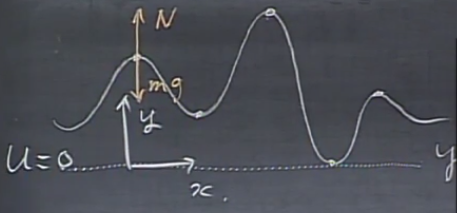
\includegraphics[scale=0.8]{Graphics/lec13_equilibrium}
\end{center}

The points along the curve have a gravitational potential energy which is $U = m g y$, since we defined $U = 0$ at $y = 0$ (the $= 0$ part is just outside the screen grab above). Since the plot is of $y = f(x)$, for some function $f$, we can also write that $U = m g f(x)$.

There are then points along this curve where $\displaystyle \frac{dU}{dx} = 0$. Those points occur where the curve's slope (or derivative) are zero, by definition, which is at the top of each peak, and at the bottom of each valley, as signified by a dot in the above figure.

From the definition we found before, that then means that $-F_x = 0$, so the net force in the $x$ direction is zero.\\
At such a point, there is a force $-m g$ in the $y$ direction, and a normal force $N = + m g$, so that there is no net force there, either.

Since there is no net force on the object at one of these points, and we can put it in such a situation at rest, it will stay exactly where it is.\\
However, there is an important difference between these two types of points  (peaks and valleys). If we try to balance a marble at the top of such a peak, just about any tiny vibration, small amount of wind etc. will get it moving. Being at the top of a large downwards slope, in either direction, it will then clearly begin to accelerate downwards -- and again, the force is in the direction of decreasing potential energy (which of course is the same thing as being in the \emph{opposite} direction as \emph{increasing} potential energy).

However, if we put a marble in one of the valleys, what happens? If there is a small force, causing a motion in any direction, it will be forced back into the valley. The force is yet again in the direction opposing the increase in potential energy, and potential energy increases both to the left \emph{and} to the right! Therfore, the force is such that the marble is returned to the middle of the valley again, to the point of lowest potential energy.

The difference between these two zero points are that the peaks provide \emph{unstable equilibrium}, while the valleys provide \emph{stable equilibrium}. If there is a disturbance in the first case, it goes out of control. In the second case, in the valleys, any small disturbance is automatically countered, and the object goes back to where it was, at the bottom.

We can find out which of these two cases a point is mathematically, by looking at the second derivative. If the second derivative of potential energy with respect to $x$ is positive, it's a point of stable equilibrium. If it is negative, it's instead a point of unstable equilibrium.

\subsection{Another look at a spring oscillator}

Let's have another look at the oscillation of a mass on a spring, this time from an energy perspective. We know that $\displaystyle U = \frac{1}{2} k x^2$, so a plot of $U(x)$ would be a parabola:

\begin{center}
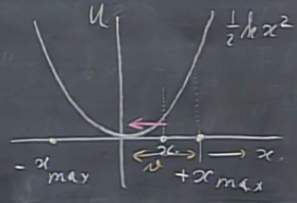
\includegraphics[scale=0.8]{Graphics/lec13_spring_pe}
\end{center}

Say we have a mass attached to a spring, as usual, and we extend it to $x_{max}$, and let it go, with zero speed.

We know that it will oscillate between $+x_{max}$ and $-x_{max}$, but we can now gain a second insight into this oscillation (albeit one mentioned earlier). Say we release the mass at an extension $x_{max}$ beyond the spring's natural length. That means the potential energy in the spring at that time is

\begin{equation}
U_{initial} = \frac{1}{2} k x_{max}^2
\end{equation}

Since we know that the force will be in the direction opposing the increase in potential energy, the mass will be pulled inwards, towards $x = 0$. Once it crosses the zero point, the force switches directions, since the current \emph{velocity} vector is towards increasing potential energy (the spring is being compressed to be shorter than its natural length). That means the force (and thus the acceleration) instantly flips over, and the mass starts slowing down. The new force is once again in the direction opposing the increase in potential energy, which is again towards $x = 0$, which is now towards the right in the figure.

Because spring forces are conservative (for ideal springs), we can use conservation of energy to write an equation for this system. The \emph{total} energy in the system must equal the spring's stored potential energy at $t = 0$, plus the mass's kinetic energy at $t = 0$. The latter is zero, since we release it at rest (zero speed), so $E_{total} = U_{initial}$. That energy must be held constant -- conservation of energy. Therefore, the sum of the mass's kinetic energy $\displaystyle \frac{1}{2} m v^2$ and the spring's stored energy $\displaystyle \frac{1}{2} k x^2$ must always equal that initial energy. We can set up an equation for this:

\begin{equation}
\frac{1}{2} m v^2 + \frac{1}{2} k x^2 = \frac{1}{2} k x_{max}^2
\end{equation}

This equation must \emph{always} hold for this system, unless there are other forces, such as friction, which we ignore for now.\\
Because $v = \dot{x}$, we can rewrite this equation a bit, by making that substitution, and getting rid of all of the one-halves, and dividing through by $m$:

\begin{align}
\frac{1}{2} m \dot{x}^2 + \frac{1}{2} k x^2 = \frac{1}{2} k x_{max}^2\\
\dot{x}^2 + \frac{k}{m} x^2 - \frac{k}{m} x_{max}^2 = 0
\end{align}

We can then take the time derivative of this. Keep in mind that since the equation is in terms of $x$, we need to use the chain rule for most terms.

\begin{align}
\frac{d}{dt} \left(\dot{x}^2 + \frac{k}{m} x^2 - \frac{k}{m} x_{max}^2\right) = \frac{d}{dt} (0)\\
2 \dot{x} \ddot{x} + 2 \frac{k}{m} x \dot{x} - 0 = 0
\end{align}

We can simplify this equation by dividing through by $2 \dot{x}$:

\begin{equation}
\ddot{x} + \frac{k}{m} x = 0
\end{equation}

Isn't it remarkable? We get the equation for simple harmonic motion, and so we find the same old solutions:

\begin{align}
x        &= x_{max} \cos(\omega t + \varphi)\\
\dot{x}  &= - \omega x_{max} \sin(\omega t + \varphi)\\
\ddot{x} &= - \omega^2 x_{max} \cos(\omega t + \varphi) = -\omega^2 x\\
\omega  )    &= \sqrt{\frac{k}{m}}\\
T           &= \frac{2 \pi}{\omega} = 2 \pi \sqrt{\frac{m}{k}}
\end{align}

\subsection{Motion of a ball along a circular track}

Say we have a circular (or at least semicircular) track of radius $R$. We define $y = 0$ and $U = 0$ to be at the bottom of the track.

\begin{center}
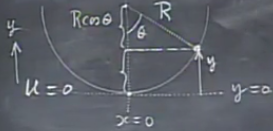
\includegraphics[scale=0.8]{Graphics/lec13_bowl}
\end{center}

When the ball is at some random location $y$, we can find the angle made with the vertical, $\theta$, via trigonemetry.\\
First, we find that the radius $R$ acts as the hypotenuse of a right triangle, where the $x$ component $R \sin \theta$ is at the bottom, and the left side has height $R \cos \theta$. Note that the $y$ coordinate fits $y = R - R\cos \theta$, so that $y = R (1 - \cos \theta)$.

With that in mind, we can write $U$ as a function of the angle $\theta$ now:

\begin{equation}
U = m g y = m g R (1 - \cos \theta)
\end{equation}

Notice that at $\theta = 0$, $U = 0$, as we defined.\\
At $\displaystyle \theta = \frac{\pi}{2}$, $U = m g R$, since it is a height $R$ above $y = 0$.

Using the definition of a radian as the arc length subtended by an angle, where $dS$ is the arc length and $d\theta$ the angle, we find

\begin{align}
\frac{dS}{R} &= d\theta\\
dS &= R d\theta
\end{align}

Taking the time derivative of both sides, we find

\begin{equation}
\frac{dS}{dt} = R \frac{d\theta}{dt} = R \dot{\theta}
\end{equation}

The left-hand term is just the distance moved per unit time, so $\displaystyle \frac{dS}{dt} = v = R \dot{\theta}$.

In most cases, we use $\displaystyle \omega = \dot{\theta} = \frac{d\theta}{dt}$, but in most cases, $\omega$ is also a constant. In this case, it is a function of the angle; the angle will change the fastest near $\theta = 0$ (at the bottom), where the speed is at a maximum, while it will change slower as the ball climbs up the ``edges'' of the circle (I think of it as a ``two-dimensional bowl''), as it is about to come to a halt, and change direction.

As a short aside, we can, as a small-angle approximation, use

\begin{equation}
\cos \theta \approx 1 - \frac{\theta^2}{2}
\end{equation}

This approximation uses the first two terms of a Taylor expansion for $\cos \theta$. If you are unfamiliar with Taylor expansions, you could look them up (even the basics are a bit too much to cover in what is already an aside). In short, they provide for a way to approximate about any function as a polynomial, or -- with an infinite amount of terms -- exactly equal those functions.

Last time we used such an approximation, we used only the first term, $\cos \theta \approx 1$. That's too inexact for this case, though -- we would end up with $U = m g R (1 - 1) = 0$ for all $\theta$!

Even for angles of about 11.5 degrees, the error caused by this approximation is way, way less than 1\% (less than 0.01\%, actually). In fact, for as much as 30 degrees, we have $\cos(\ang{30}) \approx 0.8660254$, while the approximation gives $0.862922$. It's off by about 0.3\% -- still not a lot, all things considered.

Let's return to the problem at hand. Using this approxmation, we apply the conservation of mechanical energy to this system. The total mechanical energy must be a constant. If we release the object as zero speed, and thus zero kinetic energy, the total energy (kinetic + potential) must always equal that value:

\begin{equation}
M_E = \frac{1}{2} m v^2 + m g R(1 - \cos \theta)
\end{equation}

Since $v = R \dot{\theta}$, $v^2 = R^2 \dot{\theta}^2$. Let's also apply our approximation for the cosine. What we end up with is

\begin{align}
M_E &= \frac{1}{2} m R^2 \dot{\theta}^2 + m g R(1 - (1 - \frac{\theta^2}{2}))\\
M_E &= \frac{1}{2} m R^2 \dot{\theta}^2 + m g R \frac{\theta^2}{2}
\end{align}

We can now take the time derivative of this. $M_E$ is a constant, so that becomes zero. As far the rest, we use the chain rule again:

\begin{align}
0 &= \frac{1}{2} m R^2 (2 \dot{\theta} \ddot{\theta}) + \frac{m g R}{2} 2 \theta \dot{\theta}\\
0 &= m R^2 \dot{\theta} \ddot{\theta} + m g R \theta \dot{\theta}\\
0 &= R^2 \ddot{\theta} + g R \theta
\end{align}

We can rearrange that as

\begin{equation}
\ddot{\theta} + \frac{g}{R} \theta = 0
\end{equation}

... and it is then again obvious that we have as simple harmonic oscillator! We know the solution to this differential equation, so we can write down

\begin{align}
\theta &= \theta_{max} \cos (\omega t + \varphi)\\
\omega &= \sqrt{\frac{g}{R}}\\
T      &= 2 \pi \sqrt{\frac{R}{g}}
\end{align}

Note that this $\omega$ is completely unrelated to the $\displaystyle \frac{d\theta}{dt}$ we had earlier in the derivation -- it's a good thing we didn't call that $\omega$! This one is a constant, while the other one changed with time.

Note how these equations are identical to the ones for a pendulum, that we derived earlier, also using a small-angle approximation. This time, however, it is our approximation which caused the similarity -- we made the equation quadratic in $\theta$ by doing that. The spring oscillation was quadratic in $x$ from the beginning.

Finally, on to an important detail. Nowhere in this derivation did we consider the normal force from the track on the ball. Is it really safe to ignore it? Why?

It turns out that yes, we can ignore it, because in the case of this circular track, it is always perpendicular to the direction of motion. A force perpendicular to a motion \emph{cannot} do work, because of the definition of the dot product: an angle of $\ang{90}$ between force and displacement always means zero work.

Next, a very interesting demonstration follows, that might cause some sleeplessness until we find the answer to what's going on, likely in two weeks or so.

\section{Lecture 14: Orbits and escape velocity}

As we know, the gravitational force has infinite range. Its strength at a distance is limited, though, due to the inversed square relationship. Because of this, there is a speed, the \emph{escape velocity}, that lets you escape from a body's gravitational field. That is, if you start out with that speed, you will escape it forever, even with no additional outwards force (no engines required). Of course, if you \emph{do} have engines, you certainly don't need to stay above the escape velocity the entire time to get away; all you need to do is overcome the force of the gravitational pull.

We can find this velocity for a given body (such as the Earth) quite easily, using conservation of energy. The kinetic energy at launch must be $\displaystyle \frac{1}{2} m v_{esc}^2$, and since the problem definition is that in never adds to that kinetic energy (no engines). That must therefore be the total energy of the object, at all times. The total energy at any given time is the sum of the kinetic energy at some point $r$, which we call $\displaystyle \frac{1}{2} m v_r^2$, and the potential energy at that point, $\displaystyle - \frac{G M m}{r}$, with $M$ being the mass of the Earth (or the body), and $m$ the mass of the object trying to escape.

\begin{equation}
\frac{1}{2} m v_{esc}^2 + \left(-\frac{G M m}{R_{Earth}}\right) = \frac{1}{2} m v_r^2 + \left(-\frac{G M m}{r}\right)
\end{equation}

On the left side, we have the total energy as we start out our journey, and on the right, the total energy some distance $r$ away.

However, since the goal is for the energy to be enough to escape to an infinite distance, the kinetic energy ``at'' infinity (let's just say extremely, extremely far away, since being ``at'' infinity is meaningless), the potential energy is zero, by definition. The kinetic energy is also zero, \emph{if} we gave it \emph{just} enough energy, and not any more than required (we know that the Earth's gravity will reduce the speed, and thus the kinetic energy, as time goes on).

Because of this, we can set the entire right side of the equation equal to zero, which is valid ``at'' infinity (or just so far away that the gravitational pull of the Earth is now completely negligible), and solve for the escape velocity:

\begin{align}
\frac{1}{2} m v_{esc}^2 -\frac{G M m}{R_{Earth}} = 0\\
v_{esc}^2 -\frac{2 G M}{R_{Earth}} = 0\\
v_{esc} = \sqrt{\frac{2 G M}{R_{Earth}}}
\end{align}

where, again, $M$ is the mass of the Earth. For Earth, this value is then about 11.2 km/s. So if we neglect air resistance, which will surely make these results valid if we are at the Earth's surface, if we could fire a cannon ball at more than 11.2 km/s, it would never fall back to Earth.

If the initial velocity is greater, then you will still have kinetic energy (and thus speed) left when you've escaped. In the case you do ``escape'', with the condition $E_{init} \ge 0$, you are in an \emph{unbound orbit}. In the case that $E_{init} < 0$, you enter a \emph{bound orbit}, and will never escape the gravitational pull of the Earth (or the body in question).

\subsection{Circular orbits}

Elliptical orbits will be covered later in the course, along with Kepler's laws and other fun stuff, but for now, let's introduce circular orbits, as a simplified case.

Say we have a mass $m$ orbiting the Earth, with Earth's mass being $M$, and say that $m \ll M$.\\
It moves in a circle around the Earth at constant (tangential) speed, but not constant velocity -- there is a constant centripetal accerelation, or it wouldn't be moving in a circle. Centripetal acceleration is provided by centripetal force, which in this case is the attractive force of gravity of the Earth on the mass.

We know how to find the gravitational force using the Newton's law of universal gravitation, and we can set that equal to the centripetal force $\frac{m v^2}{r}$ (which is just $a_c m$, via $F = m a$):

\begin{align}
\frac{G M m}{r^2} = \frac{m v_{orbit}^2}{r}\\
\frac{G M}{r} = v_{orbit}^2\\
\sqrt{\frac{G M}{r}} = v_{orbit}
\end{align}

where $r$ is the radius of the orbit, which has nothing to do with the radius of the Earth itself. $v_{orbit}$ is then the tangential speed of the object that is in orbit. Knowing these facts, we can now find the period of the orbit:

\begin{equation}
T = \frac{2 \pi r}{v_{orbit}} = 2 \pi \frac{r^{3/2}}{\sqrt{G M}}
\end{equation}

If we plug in the Sun's mass, and $r = \SI{149.6e9}{m}$, the approximate average distance to the sun, we find Earth's orbital period $T \approx 365.33$ days. Not bad at all, since this is only an approximation (it ignores the several things that matter, including the Earth's elliptical orbit).

As a different example, we can take the space shuttle, or the space station, which orbit at 250-400 km above the Earth's surface. If we make the calculation for 400 km, so that $r = R_{Earth} + 400$ km, we find $v_{orbit} \approx \SI{8}{km/s}$ and $T \approx 90$ minutes(!).

Note that the orbital parameters are independent on the mass of the orbiting object. It only depends on the mass of the object you orbit, and the distance from it (i.e. the radius of the orbit), times some constants.

Also note that $v_{esc} = \sqrt{2} \times v_{orbit}$, for a given point. (In $v_{esc}$, we used the radius of the Earth, because we wanted to calculate the escape velocity from the surface.)

The total mechanical energy at some radius $r$, at orbital velocity $v_{orbit}$, is

\begin{equation}
E = \frac{1}{2} m v_{orbit}^2 - \frac{G M m}{r}
\end{equation}

We can substitute the value for $v_{orbit}^2$ in there, though:

\begin{align}
E = \frac{1}{2} m \frac{G M}{r} - \frac{G M m}{r}\\
E = -\frac{1}{2} \frac{G M m}{r} = \frac{1}{2} U = - K_E
\end{align}

Quite an interesting result. In words, then, the total energy of an orbiting object is always half its gravitational potential energy, and also the negative of its kinetic energy.

Now, for something completely different (more on orbits in a few weeks).

\subsection{Power}

\emph{Power} is energy per unit time -- or work per unit time, since energy and work are closely related, and share the same dimension. The SI unit for power is joules per second, or watts, W; not to be confused with W for the quantity of work! If we have $W = $ something then it's work; if we have $P = 10$ W, then it's watts.

Stated differently, it is then just the derivative of work -- that is, $P = \displaystyle \frac{dW}{dt}$.\\
Since $dW = \vec{F} \cdot \vec{dr}$, we can take the time derivative of both sides:

\begin{equation}
\frac{dW}{dt} = \vec{F} \cdot \frac{\vec{dr}}{dt}
\end{equation}

... and since the rate of change versus time of $\vec{dr}$ is simply the velocity:

\begin{equation}
P = \vec{F} \cdot \vec{v}
\end{equation}

\subsubsection{Power in riding a bicycle}

Let's look at an example: riding a bicycle. We try to keep a constant velocity, which means there should be no net force on the bike. However, there \emph{is} air drag, and the force opposing your motion, $F_{res} \propto k v^2$. In order for there to be no \emph{net} force, your pedaling must then provide an equally great force in the forwards direction, in order for you to keep a constant speed.

As an aside, how does pedaling provide this force? First, you push down on the pedals, and the pedals push back on you with equal force via Newton's third law. This causes no net force on the bike, and we call these forces \emph{internal forces}.

The pedals push on the chain, and the chain pushes on the wheel, all of which cancels, but finally, the wheel now wants to rotate, because of the force exerted by the chain.

The wheel pushes backwards on the ground, which leads to a reaction force such that the ground pushes the wheel forward. Finally something useful! This only works because of friction, of course -- without friction, it would simply start spinning, and there would be no forward force on the bicycle.

Now, let's look at the amount of power you must provide to overcome air resistance. We can model this as a regime II problem, so the drag force is proportional to $k_2 v^2$. Say that the power you must provide at 10 miles/hour is 15 watts -- which is a given, and not something we actually show.

Now, the power we must provide is $P = \vec{F} \cdot \vec{v}$, as we showed earlier. Since the force and the velocity are in the same direction, $P = F v$. Since $F = k_2 v^2$, we find $P = k_2 v^3$! It is proportial not to $v^2$, but $v^3$.

If you then want to speed up to 25 mph, 2.5 times the original speed, you need to provide $2.5^{3} \approx 15.6$ times the power, about 230 watts! For 30 mph, 3 times the original speed, you need $3^3 = 27$ times the power (over 400 watts)! Needless to say, we reach the limits of human physiology rather quickly if we keep going like this. At 50 mph, it would take over 240 times the power (over 1800 watts -- far above what any human could do, except for elite athletes for a period of seconds or less)!

\subsection{Heat energy}

First, a few definitions. We use the symbol $Q$ for heat energy, often in the unit of calories. A calorie is the energy required to raise the temperature of 1 gram of water by 1 degree centrigrade (or 1 Kelvin, which is the same thing). There are, unfortunately, a ton of different definitions for a calorie, but all are close to 4.2 joules. (Some are defined as the energy required to heat 1 g of water from $3.5 {}^\circ$C to $4.5 {}^\circ$C, others from 14.5 to 15.5, 19.5 to 20.5, etc.)

Next, there is the \emph{specific heat} $C$, which is a constant (for a given material) that specifies the amount of energy required to raise the temperature of that material by 1 degree centigrade, per unit mass. That is, it's in $\text{cal}/(g {}^\circ\text{C})$.\\
If we want the unit to use kilograms instead of grams, which is always a nice thing when using the MKS (meter-kilogram-second) system, we simply multiply the constant by 1000.

The amount of heat energy Q, is then

\begin{equation}
Q = m C \Delta T
\end{equation}

in calories, if $m$ is in grams, $C$ in the units stated above (per gram, not per kilogram), and $\Delta T$ in either Kelvin or degrees centigrade (they are equivalent; the zero point is the only difference).\\
As a reference, ice has a specific heat of about 0.5, compared to liquid water's 1. Aluminium has a specific heat of about 0.2, and lead a very low 0.03.

James Joule first found that mechanical work and heat energy are equivalent in 1845, though he was not the first to begin research on the topic. This research, among other things, led to the naming of the joule in his honor.

\subsection{Power and the human body}

The human body radiates heat, infrared radiation, at a rate of about 100 watts -- 100 joules per second. That is about $10^7$ joules per day, which then is about 2.4 (or $\approx 2$) million calories.\\
Clearly, then, we need to input an equivalent amount of energy, or we would run dry sooner rather than later! We get this energy from food, of course.\\
Food labels are usually in kilocalories, which is sometimes written as either Cal (capital c) or kcal. They often mention the equivalent value in kilojoules as well.\\
So when a food label says 400 (kilo)calories, that that is enough for a power output of 100 watts for about 4 hours.

Normal, daily activities use almost no energy at all, compared to the rate of energy use of the body that occurs either way. Walking up 10 meters (vertically) of stairs, 5 times a day, is an average power use of about 1 W, if spread out over over 10 hours or so. That's only about 1\% of the heat energy produced by the body when essentially at rest.

On the other hand, if you climb a mountain of 5000 feet (about 1500 meters), you might do about a million joules worth of mechanical work just to overcome gravity, which is not negligible compared to the $10^7$ joules daily. In other words, you need to eat more, in order to stay the same weight (or mass, rather!).\\
Because the conversion from food energy to mechanical work is quite inefficient, eating 10\% more won't do it, though; you may have to eat 40\%+ more in order to account for the increased energy use.

\subsection{More heat, and electric energy}

Consider taking a bath: we might need to heat 100 kg of water, by about 50 degrees C. (I'm not so sure I agree with that number, though! Even if the water was $0 {}^\circ$C to begin with, it would probably be painfully hot! Anyway, let's work with the number from the lecture.)

With $C = 1 \text{ cal/(g} {}^\circ \text{C})$ for water, the answer is then simply the mass (in grams!) times $C = 1$ times 50 degrees $C$, or about $5 \cdot 10^6$ calories, which is about $\SI{2e7}{J}$.

It's fairly difficult to produce 120 watts of work in turning a crank on a generator that then produces electric energy; a student was unsuccessful, and the professor says he is also unable to do so. Still, you would need to produce those 120 watts for 48 hours in order to heat up the water in that bath by 50 degrees!

Next, a demonstration of a simple battery is shown; four cells consisting of a zinc anode and a copper cathode in a sulfuric acid solution are wired in series to power a small light bulb.

After that, some more numbers: the global energy consumption (in 1999, when the lectures were recorded) is/was about $\SI{4e20}{J}$ per year.\\
The USA consumes about 1/5 of that, with 1/30 of the world's population.

The Sun has a power output of about $\SI{4e26}{W}$, radiated in mostly visible light and infrared. Of course, it radiates a roughly equal amount in all directions, so only a small fraction of that reaches the Earth. We can calculate how large Earth's cross section is, and find the ratio of that divided by $4 \pi R^2$, with $R$ being the mean distance between the Earth and the Sun. We find about 1400 watts per square meter, that reaches the Earth's atmosphere.\\
The measured value at the ground varies greatly, for many reasons: the Sun's altitude above the horizon (i.e. day/night cycle, seasons, location on the Earth), cloud cover, and more.

If we try put solar panels on a horizontal roof, then clearly they will not do anything useful when the sun is just at the horizon.

Taking all this into account, along with solar cell inefficiency, we could perhaps provide enough energy to power the planet continously by having a 400 mile by 400 mile solar grid -- not a small area! That area is three times that of England. Clearly, we cannot sustain our current energy use by solar power alone.

Lecture question time:\\
``When the sun is in the zenith and the sky is perfectly clear, the solar power we receive on the surface of the earth is roughly 1 kW per square meter (on a horizontal surface that is normal to the direction of the sun).

Calculate the average solar power per square meter (in Watts) on a horizontal surface for a day when the sun goes through the zenith at noon.

The sun goes through the zenith exactly twice a year on latitudes that are close to the equator. Take the angle to the sun into account.''

Okay, let's see. Let's imagine one single square meter somewhere on the Earth. First we have sunrise, where the sun is at $-\pi/2$ radians compared to the zenith. At noon, it is at 0 rad (straight above), and at sunset, at $+\pi/2$ radians. The power at a given angle $\theta$ should be $P = (\SI{1000}{W})\cos\theta$. Next, we need to find an average.

We can do find the average by an integral:

\begin{equation}
\overbar{P} = \frac{1}{b - a} \int_a^b 1000 \cos \theta d \theta
\end{equation}

where $a = -\pi/2$ and $b = \pi/2$. However, that is only exactly half a day -- the other 12 hours, there is zero sunlight, so we need to divide our answer by two, which causes the additional factor of 1/2 below. We find

\begin{align}
1000 \frac{1}{\pi} \frac{1}{2} \int_{-\pi/2}^{\pi/2} \cos \theta d \theta &= \frac{1000}{2 \pi} \int_{-\pi/2}^{\pi/2} \cos \theta d \theta = \frac{1000}{2\pi} \Big[ \sin \theta \Big]_{-\pi/2}^{\pi/2}\\
                                                              &= \frac{1000}{2\pi} \times 2 = \frac{1000}{\pi} \approx \SI{318.3}{W}
\end{align}

I do believe I'm missing a simplification, but at least this gets us the correct answer.

Finally, a small note on the current energy crisis.\\
We are using fossil fuels at a rate which is about one \emph{million} times greater than nature's production. At this rate, we will run out in less than 100 years. Fossil fuels account for a bit over 80 percent of human energy consumption, so clearly we need to start producing a \emph{lot} of energy from other sources, or we will simply run out. While solar power is very useful, we have already ruled it out as a full replacement. We can combine many energy sources, though, and have solar power be one of them.

Nuclear fusion is often touted as the ``energy source of the future''. And indeed, if we can create an efficient reactor (current designs are not useable in practice, and mostly use more power than they provide back), it could provide practically limitless energy. One possible fuel source is deuterium and tritium, isotopes of hydrogen, present in sea water. We have enough water to provide the current world's energy usage for about 25 billion years, so if it could work, the energy problem would be solved.

Not only that, but fusion is both clean and intrinsically safe. Most of us know of Chernobyl or Fukushima -- rare accidents, but they do happen, and can be very problematic.\\
(Though as of late 2013, the death toll due to Fukushima is still zero (but the lifetime rate of cancer has likely increased in some people), and fission energy has a lower death rate per unit energy produced than even wind and solar energy. I'm not trying to sell some propaganda here, but I do feel that nuclear fission has a worse reputation than it deserves, even though there obviously are risks.)

If a tsunami or an earthquake were to hit a \emph{fusion} reactor, however, not a lot can happen. In magnetic containment fusion, the magnetic field would collapse if power was cut, and the reactor would automatically shut down. Not automatically as in a safety protocol, but rather without the containment, the reaction cannot be sustained, and stops all by itself. That's in contrast with a fission reactor, which must rely on safety measures to stop the reaction, so that it doesn't go out of control.\\
(Newer fission reactor designs are safer than ones in use, but few new designs are actually put into use, likely in part due the rather vocal opposition to nuclear energy.)\\
In addition, a fission reactor usually has many tons of fuel inside, while a fusion reactor can be powered off just grams of fuel, and use well below 1 ton of fuel in a year -- and the fuel is just hydrogen isotopes. Granted, tritium is radioactive, and there are some radioactive byproducts, but nowhere near the many tons a year of poisonous, radioactive material that fission reactors produce per year.

\chapter{Week 7}

\section{Lecture 15: Momentum and its conservation}

We will now introduce the concept of momentum.\\
Momentum is a vector: the product of mass and velocity. The SI units are then kg $\cdot$ m/s or N $\cdot$ s; there is no named unit for this quantity.

It is usually written as $\vec{p}$, so

\begin{equation}
\vec{p} = m \vec{v}
\end{equation}

Momentum is closely connected with force, and knowing the above, it is easy to show how. $\displaystyle F = m a = m \frac{dv}{dt}$. We can work backwards, assuming $m$ is a constant so that $m \frac{dv}{dt} = \frac{d(mv)}{dt}$:

\begin{equation}
F = m \frac{dv}{dt} = \frac{d(mv)}{dt} = \frac{dp}{dt}
\end{equation}

So force is the time derivative of momentum.\\
This also implies that in order for an object's momentum to change, a force must have acted on it. And, conversely, if a (net) force acts on an object, its momentum must change.

Next, the professor shows (in some detail) how momentum is conserved for a \emph{system} of particles/objects, unless there is a net \emph{external} force on them. What happens internally does not matter, since all such internal forces cancel out, when you consider the system as a whole. For example, if two particles collide, the momentum of both particle \#1 and of particle \#2 may change, but the momentum of \#1 + \#2 will stay a constant.

This then leads to the \emph{conservation of momentum}, which is a very helpful concept in solving some kinds of problems. Let's solve a simple problem using this principle.

Say we have two objects of masses $m_1$ and $m_2$ respectively, both moving towards the right, with velocities $v_1$ and $v_2$, where $v_1 > v_2$. Eventually, the two will collide.

Momentum prior to the collision can be found by the sum $m_1 v_1 + m_2 v_2$; since it is a vector, it has a direction. Both velocities are towards the right, so the net momentum will be as well; we take right to be increasing value of $x$, so that the numbers are positive.

In the collision, the masses will stick together -- pretend that we put glue on one of them. (Collisions where the two separate after colliding are covered later in the lecture, or in the next.)\\
Because they stick together, they will share a velocity later -- and a momentum, as well. The momentum after the collision can be written as $(m_1 + m_2) v'$, if we call the new velocity $v'$. 

Via conservation of momentum, the two must be equal, if there are no external forces (so this collision happens on a frictionless table, with no air drag etc). We set them equal, and solve for $v'$:

\begin{align}
(m_1 + m_2) v' &= m_1 v_1 + m_2 v_2\\
v' &= \frac{m_1 v_1 + m_2 v_2}{m_1 + m_2}
\end{align}

To get a feeling for this, say $m_1 = \SI{1}{kg}$, $m_2 = \SI{2}{kg}$, $v_1 = \SI{5}{m/s}$ and $v_2 = \SI{3}{m/s}$. Mass 1 has a momentum of $\SI{5}{kg m/s}$, while mass 2 has $\SI{6}{kg m/s}$. The net momentum prior to the collision is then $\SI{11}{kg m/s}$, since the two are in the same direction.

Both velocities are towards the right and thus positive, so $v'$ will also be positive.\\
Plugging the numbers in, we find $\SI{11/3}{m/s}$ as the new velocity for the masses, moving together.

What is now the momentum? It is the new velocity times the total mass, which is $(11/3) \times 3$, so indeed we find that momentum was conserved. Not a huge surprise, since we derived the equation from that assumption!

What may be surprising is instead what happens to the kinetic energy.\\
Prior to the collision, the total kinetic energy was 12.5 J + 9 J = 21.5 J.

After the collision, the total kinetic energy is only $20.1\overbar{6}$ J -- we lost one and a quarter of a joule. Not a whole lot, perhaps, but let's look at a second situation.

Say we have the same values for the masses and velocities, only that $v_2$ is now negative, i.e. to the left, and so the two hit each other head-on.

Mass 1 still has the same momentum of $\SI{5}{kg m/s}$, but $v_2$ now has $-\SI{6}{kg m/s}$. The net momentum is now $\SI{-1}{kg m/s}$ instead of +11.

Using the same formula, we now find $v' = -1/3$ m/s. The initial kinetic energy is unchanged -- the masses are the same, and the \emph{speeds} are the same -- but the kinetic energy after the collision is now a tiny 1/6 of a joule!

In short: in the absence of (net) external forces, the momentum of a \emph{system} of two or more objects is always conserved; kinetic energy, however, is not.

Let's have a look at a two-dimensional problem from a lceture question:

``In a scattering experiment, an incident alpha particle of mass $M_1 = 4u$ interacts with a static proton of mass $M_2 = u$. The incident particle is initially moving along the x-axis with a velocity $\vec{v_1} = v_{1x} \hat{x} = 0.05 c \hat{x}$, and a final velocity (after collision) $\vec{v_1}' = v_{1x}^{'} \hat{x} + v_{1y}^{'} \hat{y} = 0.044 c \hat{x} + 0.008 c \hat{y}$, where $c$ is the speed of light ($c = \SI{3e8}{m/s}$).

What is the speed of the proton after the collision?\\
What is the direction of the proton after the collision? (give the angle with respect to the x-axis in radians)''

Haha, honestly, I was stuck for a while, since I found one equation with two unknowns, for each component, so total two equations, four unknowns. It turns out that half of those ``unknowns'' are part of the question, only I didn't realize at first. Duh!

To solve this, we apply conservation of momentum on the two axes, independently of each other.\\
Before and after the collision, in the $x$ direction:

\begin{align}
4 u v_{1x} = 4 u v_{1x}^{'} + u v_{2x}^{'}\\
4 (v_{1x} - v_{1x}^{'}) = v_{2x}^{'}
\end{align}

where $v_{2x}^{'}$ is the $x$ component of the proton's velocity after the collision. Plugging in the numbers given, we find $v_{2x}^{'} = 4(0.05c - 0.044c) = 0.024c$.

Next, the $y$ direction. Neither particle has any $y$ component whatsoever at the moment, so the net momentum prior to the collision is clearly zero. That also means that the net momentum \emph{after} the collision must be zero.

\begin{align}
4 u v_{1y}^{'} + u v_{2y}^{'} = 0\\
v_{2y}^{'} = -4 v_{1y}^{'}
\end{align}

So we find $v_{2y}^{'} = -0.032c$.

With that in mind, we can now calculate the speed as $v_2^{'} = \sqrt{(v_{2x}^{'})^2 + (v_{2y}^{'})^2} = 0.04c$.

Next up, the angle made with the $y$ axis. If we consider the components, it must be angled downwards to the height. Drawing it out, we find that

\begin{equation}
\theta = \arctan \frac{v_{2y}^{'}}{v_{2x}^{'}} = \arctan \frac{-0.032}{0.024} = \ang{-53.13}
\end{equation}

This angle would put it in the correct quadrant, and since the magnitude of the $y$ component is slightly greater than that of the $x$ component, it makes sense that the angle is a bit more than a 45 degrees down from the axis.

Next, there is a great demonstration of the conservation of momentum. I didn't take any notes of it, however.

\subsection{Center of mass}

Every object, regardless of shape or size, has a center of mass; a single point, which has some very interesting and useful properties.

We take any object, of any size (greater that zero, however, or the entire point is lost), and think of it as being composed by a practically infinite amount of small masses $m_i$. Each mass has a position vector $\vec{r_i}$ from the origin, which we are free to choose.

\begin{center}
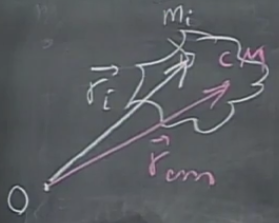
\includegraphics[scale=0.7]{Graphics/lec15_cm}
\end{center}

It is then true that the 

\begin{align}
M_{tot} \vec{r_{cm}} &= \sum_i m_i \vec{r_i}\\
\vec{r_{cm}} &= \frac{1}{M_{tot}} \sum_i m_i \vec{r_i}
\end{align}

In the limit as the masses become infinitesimally small, this becomes an integral:

\begin{align}
\vec{r_{cm}} &= \frac{1}{M_{tot}} \int \vec{r} \mathop{dm}
\end{align}

$x$, $y$ and $z$ components of this can be found in the same way, with three separate integrals.

For the simple case of two particles along a single axis:

\begin{equation}
x_{cm} = \frac{m_1 x_1 + m_2 x_2}{m_1 + m_2}
\end{equation}

This gives a result where the center of mass is closer to the more massive of the two objects. If they are equally massive, the center of mass is at the midpoint between the two.

Returning to the first equation solved for $\vec{r_{cm}}$, we can take the time derivative of both sides of this equation. $\vec{r_{cm}}$ becomes $\vec{v_{cm}}$, and $\vec{r_i}$ becomes $\vec{v_i}$, since velocity is the time derivative of position.

\begin{equation}
\vec{v_{cm}} = \frac{1}{M_{tot}} \sum_i m_i \vec{v_i}
\end{equation}

However, note that $\sum_i m_i \vec{v_i}$ is the sum of the mass-velocity products: it is the total momentum of the system. In other words,

\begin{align}
\vec{v_{cm}} &= \frac{1}{M_{tot}} \vec{p_{tot}}\\
\vec{p_{tot}} &= M_{tot} \vec{v_{cm}}
\end{align}

This second result is an important one: the total momentum of a system can be found by knowing its total mass and the velocity of its center of mass, and is the same regardless of what the rest of the system is doing.

Not only that, but we can take the time derivative of this. The time derivative of momentum is force (or net external force, to be more precise), while the derivative of velocity of the center of mass is the \emph{acceleration} of the center of mass:

\begin{equation}
F_{ext} = M_{tot} \vec{a_{cm}}
\end{equation}

This is a very interesting result. Regardless of the shape of an object, if we know the external force and the total mass, we can predict how the center of mass moves in a simple way, even though the motion of the object as a whole may be very complicated and involve tumbling/spinning at varying speeds, etc.

So if the (net) external force is zero, the center of mass will continue to move in a straight line, forever, regardless of what the rest of the object is doing.

\section{Lecture 16: Elastic and inelastic collisions}

Last lecture was focused on inelastic collisions; we will now consider general collisions, including elastic ones. Again, let's start with a one-dimensional example.

A mass $m_1$ is moving towards the right with speed $v_1$, towards a mass $m_2$ which is at rest. We take increasing values of $x$ to be towards the right.

After the collision, $v_1^{'}$ can be either positive or negative (to the right or to the left), while $v_2^{'}$ is certainly towards the right. (If an object hits it from the left, how could it start moving towards the left?)

To find the velocities after the collision, we can apply conservation of momentum. Only the first mass had any momentum prior, so that must be the sum of the momentum after the collision as well:

\begin{equation}
m_1 v_1 = m_1 v_1^{'} + m_2 v_2^{'}
\end{equation}

Unfortunately, the equation has two unknowns; we need a second equation to get anywhere.

In order to find a second equation, we can use the conservation of energy. \emph{Kinetic} energy is not necessarily conserved in collisions, which we saw last lecture. However, the kinetic energy that is lost must be converted to some other form of energy, such as heat energy.

If we use an extra $Q$ to denote the rest of the energy, we can write an equation of the form $K + Q = K'$, where $K$ is the kinetic energy prior to the collision, and $K'$ is the kinetic energy after.

There are three possible cases here.

\begin{itemize}
\item $Q > 0$: we call this a \emph{superelastic} collision; the amount of kinetic energy has \emph{increased} (as demonstrated with a spring's stored energy as the source in the previous lecture; an explosion or such could also cause this to happen).
\item $Q = 0$: this is an \emph{elastic} collision (or ``completely elastic''; the modifier ``completely'' is really not necessary, however). Kinetic energy is \emph{conserved} in this special case.
\item $Q < 0$: this is an inelastic collision. Kinetic energy is lost in the collision (in any amount from almost none lost, to \emph{all} kinetic energy lost), and is mostly turned into heat (but perhaps also noise and vibration, etc).
\end{itemize}

Let's focus on the special case of elastic collision, so that $Q = 0$ and $K = K'$. In this case, we can write an equation relating the initial kinetic energy to the final kinetic energy, as follows:

\begin{align}
\frac{1}{2} m_1 v_1^2 &= \frac{1}{2} m_1 (v_1^{'})^2 + \frac{1}{2} m_2 (v_2^{'})^2\\
m_1 v_1^2 &= m_1 (v_1^{'})^2 + m_2 (v_2^{'})^2
\end{align}

Combining this with the equation that relates the momentum of the system, we can find expressions for $v_1^{'}$ and $v_2^{'}$ as follows, by solving the system of equations:

\begin{align}
v_1^{'} &= \left(\frac{m_1 - m_2}{m_1 + m_2}\right) v_1\\
v_2^{'} &= \left(\frac{2 m_1}{m_1 + m_2}\right) v_1
\end{align}

So the above is valid under three conditions: the initial velocity $v_2 = 0$ initially, $Q = 0$ and momentum is conserved (i.e. there is no net external force on the system).

We will now look at what will happen in three special cases: $m_1 \gg m_2$, $m_1 \ll m_2$ and $m_1 = m_2$.

First out is $m_1 \gg m_2$, which turns out to be the same as $m_2 \to 0$. What happens in the above equations as $m_2 \to 0$?

Well, $v_1^{'} = v_1$ -- which comes as no surprise. If a very massive object runs in to one that has practically zero mass, it will just continue on its way.\\
What happens to the smaller object is more interesting: its velocity goes to $v_2^{'} = 2 v_1$. As long as $m_1 \gg m_2$, no matter what the actual masses or velocities are, it will zoom away at twice the speed of the object that hits it.

Next, the opposite case, where $m_1 \ll m_2$, which means $m_1 \to 0$. Since $m_1$ is the one that moves initially, I would expect it to change direction and move backwards at some speed, while $m_2$ does almost nothing. Let's plug it in: we find $v_1^{'} = -v_1$ and $v_2^{'} = 0$, as predicted. It turns out that $m_1$ simply bounces back with the \emph{same} speed, only in the opposite direction. Considering what happened to the tiny mass in the previous case, this might not be obvious -- it was twice the speed in the previous case!

Finally, what happens if the masses are about the same? Plugging it in, we find $v_1^{'} = 0$, and $v_2^{'} = v_1$: the first object stops, and the second moves as the first one did prior to the collision.\\
Most have seen this in action, perhaps while playing pool, or in a ``Newton's cradle'' where several balls (usually at least 3, but 2 works) hang suspended as pendula; you raise one up, and when it whacks on the rest, only the one at the other end starts moving; the others merely ``relay'' the momentum through until it reaches the last ball.

The cases where $m_1 = m_2$ and $m_1 = 0.5 m_2$ are then demonstrated, with very convincing results!

What if $v_2 \neq 0$? More specifically, $v_2 > 0$, so that they are both moving towards the right, with $v_1 > v_2$ so that they will eventually collide. Again, we assume an elastic collision.

If we set up the system of equations, with the change that both masses now have momentum towards the right, and both have initial kinetic energy, we find 

\begin{align}
v_1^{'} &= \frac{m_1 v_1 - m_2 v1 + 2 m_2 v_2}{m_1 + m_2}\\
v_2^{'} &= \frac{2 m_1 v_1 - m_1 v_2 + m_2 v_2}{m_1 + m_2}
\end{align}

With $m_1 = m_2$, this yields a funny result: the two essentially trade speeds with one another. $v_1^{'} = v_2$ and $v_2^{'} = v_1$.

\subsection{Elastic collisions seen from the frame of the center of mass}

We can choose our reference frame such that the center of mass has zero velocity in our frame. This is referred to as the ``center of mass frame'', ``center of momentum frame'' or COM frame.

In this frame, total momentum is always zero. We found last lecture that $\vec{p_{tot}} = M_{tot} \vec{v_{cm}}$, and \emph{in the COM frame}, $v_{cm} = 0$ by definition. That definition is what makes it the COM frame.

Using the definition for the velocity of the center of mass

\begin{equation}
v_{cm} = \frac{1}{M_{tot}} \sum_i m_i v_i = \frac{\sum_i m_i v_i}{\sum_i m_i}
\end{equation}

and a Galilean transformation for the velocities of two particles,

\begin{align}
u_1 &= v_1 - v_{cm}\\
u_2 &= v_2 - v_{cm}
\end{align}

where the $u$ notation is used for the particle's velocities in the COM frame, we can show that the total momentum must be zero in this frame, in a different way.

The sum $\sum_i m_i u_i$ is the net momentum in the COM frame. $u_i = (v_i - v_{cm})$, so we substitute that in and find $\sum_i m_i (v_i - v_{cm})$ as the total momentum. Using the definition of $v_{cm}$ above, that is

\begin{equation}
\sum_i m_i \left(v_i - \frac{\sum_i m_i v_i}{\sum_i m_i}\right) = \sum_i m_i v_i - \sum_j m_j \frac{\sum_j m_j v_j}{\sum_j m_j} = 0
\end{equation}

The denominator in the fraction becomes $1$, and we then have the subtraction of two equal quantities that equals the total momentum, as seen from the COM frame, since the indices $i$ and $j$ are equivalent.

Now that we can hopefully accept the above as being true (I had trouble seeing it until I did the above)...\\
Say we are in this frame, and there are two particles with velocities inward toward the center of mass; one mass $m_1$ with speed $u_1$, and one mass $m_2$ with speed $u_2$ -- again with those speeds being in the COM frame. Also say $Q = 0$ for this collision, i.e. it is an elastic collision.

Momentum is zero both before and after the collision. In addition, because this is an elastic collision, we can also write down an equation relating kinetic energy before and after the collision. Altogether, we have:

\begin{align}
m_1 u_1 + m_2 u_2 &= 0\\
m_1 u_1^{'} + m_2 u_2^{'} &= 0
\end{align}
\begin{equation}
\frac{1}{2} m_1 u_1^2 + \frac{1}{2} m_2 u_2^2 = \frac{1}{2} m_1 (u_1^{'})^2 + \frac{1}{2} m_2 (u_2^{'})^2
\end{equation}

With all this information, we can find (through some tedious algebra) two very simple answers: $u_1^{'} = -u_1$ and $u_2^{'} = -u_2$.

That is, \emph{as seen from the center of mass frame}, which is moving, both simply reverse direction, but keep moving at the same speed. This happens regardless of the masses and speeds, so this is clearly only possible in this very special frame.

In this simple case with only two objects, the definition we have above for $v_{cm}$ is fairly simple:

\begin{equation}
v_{cm} = \frac{m_1 v_1 + m_2 v_2}{m_1 + m_2}
\end{equation}

We can then follow the process of first transforming our velocities into velocities as seen from the center-of-mass by subtracting $v_{cm}$, do the collision calculations knowing that momentum is zero both before and after the collision (this holds for all collisions; inelastic, elastic and superelastic), and then transforming back to the external frame by \emph{adding} $v_{cm}$ back.

Since the center of mass moves at a constant velocity in the absence of external forces, we need not worry about it having changed during the collision (unless we are making an incorrect assumption that the external forces are zero).

Let's try an example (from a lecture question).

``Before a 1-dimensional collision, two masses $m_1 = 3$ kg and $m_2 = 5$ kg have velocities $v_1 = -5$ m/s and $v_2 = 3$ m/s with respect to their center-of-mass frame.

What are their velocities (in m/s) in the laboratory frame after an elastic collision? (The velocity of the center of mass is $v_{cm} = 2$ m/s)''

Alright, so in the center of mass frame, $v_1^{'} = 5$ m/s and $v_2^{'} = -3$ m/s, since all they do in that frame is reverse direction. To convert this to the lab frame, we need to \emph{add} $v_{cm}$ to these numbers, so we find 7 m/s and -1 m/s, respectively. That was certainly very easy.

\subsection{Inelastic collisions seen from the center of mass frame}

The center of mass frame has another interesting property. In the case of a completely inelastic collision, i.e. the two masses that collide stick together, both velocities go to zero (as seen from the center of mass; this would be true even if they were sliding together according to an outside observer).\\
Zero velocity means zero kinetic energy, so \emph{all} kinetic energy will be lost in this frame.

This kinetic energy, as seen from the center of mass frame, is called the \emph{internal energy}; it is the maximum energy that can be converted to heat in a collision.

Let's first calculate the amount of kinetic energy lost in a completely inelastic collision, as seen from the ``lab frame'' (one that is fixed to the room you're in, i.e. what at least I personally would consider the default frame).

We take the case where a mass $m_1$ moves with speed $v_2$ towards a second mass, $m_2$, that is at rest (with respect to the lab frame). It's a completely inelastic collision, so they stick together after the collision.

After the collision, we call the velocity $v'$ (which is just a speed in the same direction as $v_1$, since momentum is conserved), and the total mass is then $m_1 + m_2$.\\
Conservation of momentum gives

\begin{equation}
m_1 v_1 = (m_1 + m_2) v'
\end{equation}

\begin{equation}
v' = \frac{m_1 v_1}{m_1 + m_2}
\end{equation}

$v_{cm} = v'$; that can be seen very easily by looking at the equation for $v_{cm}$, and considering the case where $v_2 = 0$, as it is here. $v_{cm}$ equals exactly the above expression in that case.

Next, we can calculate the difference is potential energy before ($K$) and after ($K'$) the collision. This is the $Q$ we had in a previous equation (see the note just below; I made a small mistake):

\begin{align}
Q = K' - K &= \frac{1}{2} m_1 v_1^2 - \frac{1}{2} (m_1 + m_2) \left(\frac{m_1 v_1}{m_1 + m_2}\right)^2\\
           &= \frac{1}{2} m_1 v_1^2 - \frac{m_1^2 v_1^2}{2(m_1 + m_2)}\\
           &= \frac{m_1 v_1^2(m_1 + m_2)}{2(m_1 + m_2)} - \frac{m_1^2 v_1^2}{2(m_1 + m_2)}\\
           &= \frac{m_1 v_1^2(m_1 + m_2) - m_1^2 v_1^2}{2(m_1 + m_2)}\\
           &= - \frac{m_1 m_2}{2(m_1 + m_2)} v_1^2 \text{ (see below re: minus)}
\end{align}

Phew! This is then, from the external reference frame, the amount of kinetic energy lost in the collision.\\
As it turns out, I accidentically calculated $K - K'$ instead. The only difference is a minus sign, of course, so the actual answer should be \emph{minus} what I actually found; I added the sign in the last step above, instead of re-writing the code for this mess; sorry about that.\\
So the last line in the equation above is correct.

Next, we do the same calculation in the center of mass frame. We know $v_{cm}$, $v_1$ and $v_2$, so we can jump straight to converting the velocities. Using $u_i$ for the velocities as seen from the center of mass frame,

\begin{align}
u_1 &= v_1 - v_{cm} = v_1 - \left(\frac{m_1 v_1}{m_1 + m_2}\right)\\
u_2 &= v_2 - v_{cm} = - \left(\frac{m_1 v_1}{m_1 + m_2}\right)
\end{align}

The first equation simplifies:

\begin{align}
u_1 &= \frac{v_1(m_1 + m_2) - m_1 v_1}{m_1 + m_2}\\
u_1 &= \frac{v_1 m_1 + v_1 m_2 - m_1 v_1}{m_1 + m_2}\\
u_1 &= \frac{v_1 m_2}{m_1 + m_2}
\end{align}

And we can then write them as

\begin{align}
u_1 &= \left(\frac{m_2}{m_1 + m_2}\right) v_1\\
u_2 &= - \left(\frac{m_1}{m_1 + m_2}\right) v_1
\end{align}

We can then calculate the total kinetic energy \emph{prior} to the collision as

\begin{align}
K &= \frac{1}{2} m_1 u_1^2 + \frac{1}{2} m_2 u_2^2\\
K &= \frac{1}{2} m_1 \left(\left(\frac{m_2}{m_1 + m_2}\right) v_1\right)^2 + \frac{1}{2} m_2 \left(- \left(\frac{m_1}{m_1 + m_2}\right) v_1\right)^2\\
K &= \frac{1}{2} m_1 \left(\frac{v_1 m_2}{m_1 + m_2}\right)^2 + \frac{1}{2} m_2 \left(\frac{v_1 m_1}{m_1 + m_2}\right)^2\\
K &= \frac{v_1^2 m_1 m_2^2}{2(m_1 + m_2)^2} + \frac{v_1^2 m_2 m_1^2}{2(m_1 + m_2)^2}\\
K &= \frac{v_1^2 m_1 m_2^2 + v_1^2 m_2 m_1^2}{2(m_1 + m_2)^2}\\
K &= \frac{(m_1 + m_2) m_1 m_2 v_1^2}{2(m_1 + m_2)^2}\\
K &= \left(\frac{m_1 m_2}{2(m_1 + m_2)}\right) v_1^2
\end{align}

Again, phew! Note that this is exactly the same as the answer we found earlier, for the kinetic energy lost in the lab frame.\\
In this frame, that energy is \emph{all kinetic energy that exists to begin with}. After the collision, kinetic energy will be zero, since the wreck sticks together (this entire section is about a completely inelastic collision), and neither body will move with respect to the center of mass after the collision.\\
In other words, the \emph{change} in kinetic energy is the same in both reference frames, even though the initial and final energies are different in the different frames.

Lecture question time.

``Just before an inelastic head-on collision, two cars have a relative speed of $v = 40$ km/h (25 mph). The cars have masses $m_1 = 1300$ kg and $m_2 = 1600$ kg.\\
How much kinetic energy is lost during the collision?''

Hmm. Well, we can use the equation above. Assume $v_2 = 0$, and then it's just a matter of sticking the numbers in there, which yields about 44300 J.

\section{Lecture 17: Momentum of individual objects}

Previously, we measured the speed of a bullet, simply by measuring how long it took the bullet to move a certain distance. This was only possible because of the electronic timer, which both started and stopped automatically, as the bullet was shot through two wires.\\
We will now calculate the speed, by a more manual, indirect method, of firing the bullet into a block hanging as a pendulum. This way, we can find the velocity (with a fairly large uncertainty, but still) with nothing but a small meter stick and knowledge of physics.

The way in which we do this is fairly complex, but let's start simple. We have a solid block of mass $M$ hanging from a string of length $\ell$; this forms a \emph{ballistic pendulum}.

The bullet of mass $m$ comes in with a velocity $v$, and ``merges'' with the block (gets stuck inside), so we can model this is a completely inelastic collision. The block moves from its equilibrium position (straight down), towards the right and slightly upwards (since it is a pendulum!), with velocity $v'$.

We can apply conservation of momentum to find $v'$:

\begin{align}
m v &= (m + M) v'\\
v' &= \frac	{m v}{m + M}
\end{align}

Soon thereafter, $v'$ will have gone to zero, as the pendulum reaches its highest point. Here, we know that kinetic energy is zero, and all kinetic energy has been converted into gravitational potential energy.\\
If we define $U = 0$ at the equilibrium position, the change in gravitational potential energy was $(m + M) g h$, where $h$ is the amount the block moved upwards. This energy must have come from the kinetic energy, so via conservation of energy, we can relate the block's initial kinetic energy (as the bullet is absorbed) and the gravitational potential energy as it stops:

\begin{equation}
\frac{1}{2} (m + M) (v')^2 = (m + M) g h
\end{equation}
\begin{equation}
v' = \sqrt{2 g h}
\end{equation}

With this in mind, we could theoretically fire a bullet into the block, measure how far it moves up, and calculate the speed of the bullet. However, the upwards movement is miniscule, less than a single millimeter; we still cannot measure that with any useful accuracy. We \emph{can} measure how far it travels towards to the side, though, since that excursion is must greater. (Remember how we even neglected the upwards motion of a pendulum completely when we derived an equation for it using simple harmonic motion?)

So if we set the origin at the equilibrium position, we can call the maximum horizontal displacement of the pendulum $x$. Via trigonometry, we can find that $x = \ell \sin \theta$, and $h = \ell - \ell \cos \theta = \ell(1 - \cos \theta)$.

Using the same small-angle approximations we have used previously, that $\displaystyle \cos \theta \approx 1 - \frac{\theta^2}{2}$ and $\sin \theta \approx \theta$ (both only valid for radians), $\displaystyle h \approx \ell \frac{\theta^2}{2}$.

For $\ell = 1$ meter and $\theta = \ang{2}$, we find that $h \approx 0.6$ mm, far to small to measure with any useful accuracy. However, $x \approx \ell \theta \approx 3.5$ cm, which is much more reasonable. 

Since we now know $x$ as a function of $\theta$, we can write $h$ as a function of $x$ by combining the two equations:

\begin{equation}
h \approx \ell \frac{\theta^2}{2} \approx \frac{\ell}{2} \left(\frac{x}{\ell}\right)^2 = \frac{x^2}{2 \ell}
\end{equation}

With this in mind, we can find $v'$ as a function of $x$

\begin{equation}
v' = \sqrt{2 g} (\frac{x}{\sqrt{2 \ell}}) = x \sqrt{\frac{g}{\ell}}
\end{equation}

... and then finally the bullet's original velocity $v$ as a function of $v'$, by using the old conservation of momentum equation we had:

\begin{equation}
v = \frac{v'(m + M)}{m} = x \frac{m + M}{m} \sqrt{\frac{g}{\ell}}
\end{equation}

Let's now look at some numbers. The mass of the bullet is $m = \SI{2.0(2)}{g}$; $M = \SI{3.20(2)}{kg}$, and $\ell = \SI{1.13(2)}{m}$.

With these numbers, we find $v = 4.7 \times 10^{3} x$. The total uncertainty is somewhere around 15\%, in large part because of the large uncertainty in $m$.

When the experiment is carried out, $x \approx \SI{5.2}{cm}$ = 0.052 meters, so $v \approx \SI{244}{m/s}$. Of course, with a 15\% uncertainty, that last four may be rather meaningless. 15\% less than this is just 207.5 m/s, and 15\% more is 280.5 m/s.

Comparing the initial kinetic energy of the bullet $\displaystyle \frac{1}{2} m v^2 \approx 59.5$ J (with a large uncertainty) and the maximum kinetic energy of the block-bullet system $\displaystyle \frac{1}{2} (m + M) (v')^2 \approx 0.038$ J, we see that the vast majority of the kinetic energy was lost to heat, deforming the block (and perhaps bullet), etc. About 99.94\% was lost, according to the lecture, which seems to match this calculation quite well.

\subsection{Impulse}

Impulse is a concept closely related to momentum. Any time a change in momentum occurs for an object, an impulse was imparted on that object.\\
It is a vector, and can be written as the time integral of force:

\begin{equation}
\vec{I} = \int_{t_0}^{t_1} \vec{F} \mathop{dt} = \int_0^{\Delta t} \vec{F} \mathop{dt}
\end{equation}

using $\Delta t = t_1 - t_0$. In the simple case where the force is constant, $\vec{I} = \vec{F} \Delta t$.

However, force is also the rate of change of momentum. Therefore, the integral above can also be written as the integral of the derivative of momentum -- clearly, the dimension here is going to be the same as that of momentum.\\
In fact, we can show that the impulse is just the difference in momentum at two different times; using $\vec{p_i}$ for the initial momentum and $\vec{p_f}$ for the final momentum, 

\begin{equation}
\vec{I} = \vec{p_f} - \vec{p_i}
\end{equation}

The units of impulse are then the same as those of momentum: kg m/s or newton-seconds ($N \cdot s$).

As an example, take the collision of a ball bouncing on the floor. In the simple case where the collision is elastic, and the ball bounces back to the same height (which is of course impossible, but we can come close), the ball hits the floor with momentum $m v$, if we take downwards to be the positive direction, and leaves with equal momentum in the opposite direction, that is, $- m v$.

The impulse is then found as $- mv - (mv) = - 2 m v$. The impulse is upwards in this case, and has the magnitude of the change in momentum $2 m v$.

In the case of a completely inelastic collision (in other words, no bounce), as with a tomato hitting the floor, the impulse is smaller in magnitude at just $m v$ -- the colliding object loses all of its momentum to the floor, and ends up with zero speed and zero momentum.

Using the definition of impulse in terms of force, we can calculate the average force on a body during a collision as

\begin{equation}
\Braket{F} = \frac{I}{\Delta t}
\end{equation}

As an example, a ball (bouncy ball, super ball or what you may call it) with a mass $m = 0.1$ kg is dropped from a height of 1.5 meters. That gives it a speed of about 5.5 m/s (a bit less) as it hits the floor. Assuming an elastic collision, $I = 2 m v = 1.1$ kg m/s.\\
We can then divide this by the impact time to find the average force. The impact time was measured (by high-speed photography) to be just 2 milliseconds. That gives an average force of

\begin{equation}
\Braket{F} = \frac{\SI{1.1}{kg m/s}}{\SI{0.002}{s}} = \SI{550}{N}
\end{equation}

Remember that our definition (at least one definition) of \emph{weight} was the magnitude of the normal force exerted by e.g. the floor, to counteract gravity. (It could also be the tension in a rope, pulling you upwards.)

That means that this ball, during the short moment of the collision, has a weight about 550 \emph{times} greater than it would otherwise ($550 g$), since its ``normal'' weight is just $m g \approx 1$ N (a bit less, but we use $g \approx \SI{10}{m/s^2}$ for simplicity).

Lecture question time:\\
Car 1 of mass $m_1$ is moving along the +$x$-axis with speed $v_1$ towards car 2 of mass $m_2$ and speed $v_2$ moving along the -$x$-axis. They have a head-on collision that lasts a time interval $\Delta t$. After the collision the cars stick together. (Note: $m_1$ and $m_2$ include the drivers.)

The magnitude of the average force acting upon the driver of mass $m_{dr1}$ in car 1 by her seat belt during the collision is given by:

\begin{align}
F_{dr1} &= \frac{m_1}{m_1 + m_2} (v_1 - v_2) \frac{m_{dr1}}{\Delta t}\\
F_{dr1} &= \frac{m_1}{m_1 + m_2} (v_1 + v_2) \frac{m_{dr1}}{\Delta t}\\
F_{dr1} &= \frac{m_2}{m_1 + m_2} (v_1 - v_2) \frac{m_{dr1}}{\Delta t}\\
F_{dr1} &= \frac{m_2}{m_1 + m_2} (v_1 + v_2) \frac{m_{dr1}}{\Delta t}
\end{align}

If $v_1 = v_2$, considering the two are \emph{speeds} in opposite directions, the driver will most certainty not experience zero force, so the two options with minus signs should both be wrong. Still, let's solve this the proper way.

Total momentum is conserved, and the cars stick together. Considering that $v_2$ is towards the $-x$ axis, its velocity is negative, so the sum of momenta becomes a subtraction. The velocity after the collision is given by

\begin{align}
m_1 v_1 - m_2 v_2 = (m_1 + m_2) v'\\
v' = \frac{m_1 v_1 - m_2 v_2}{m_1 + m_2}
\end{align}

The driver's initial and final speeds are the same as the car's, of course. With that in mind, we can calculate the impulse of the driver directly, as

\begin{align}
I &= m_{dr1} v' - m_{dr1} v_1\\
I &= m_{dr1}  \frac{m_1 v_1 - m_2 v_2}{m_1 + m_2} - m_{dr1} v_1\\
I &= - \frac{m_2(v_1 + v_2)}{m_1 + m_2} m_{dr1}
\end{align}

We wanted a magnitude, but got a negative number; that is simply due to the coordinate system choice. Since all variables must be positive ($v_1$ and $v_2$ are speeds and never negative), we can simply remove the minus sign to find the magnitude.

By definition, $\Braket{F} \Delta t = I$, so we can write this in terms of an average force. We just make that substitution, and solve for the force by dividing both sides by $\Delta t$:

\begin{equation}
\Braket{F} = \frac{m_2(v_1 + v_2)}{m_1 + m_2} \frac{m_{dr1}}{\Delta t}
\end{equation}

Finally, we have one of the four possible answers, and it is indeed the correct one.

Next up, we have some talk about impact times, though nothing general enough to really write down. As always, no notes doesn't mean not worth watching -- it's really a bit of the opposite.

\subsection{Thrust and rockets}

Consider the case of throwing tomatoes towards the floor again. Say we throw $n$ tomatoes per second, and each tomato has a mass $m$. $n m$ is (tomatoes/second) times (kilograms/tomato), so the dimension of this is in kilograms per second of ``stuff'' we throw.

The change in momentum for each tomato is $m v$; $n m v$ gives us the dimension of impulse per time, so

\begin{equation}
n m v = \frac{\Delta p}{\Delta t} = \Braket{F}
\end{equation}

Since $\displaystyle \frac{dp}{dt}$ is the definition of force, the above yields a time-averaged force. The floor experiences a net downwards force from all these tomatoes.

In the form of a proper derivative, we have

\begin{equation}
F = \frac{dm}{dt} v
\end{equation}

Similarly, in the case of a more horizontal case, we need to accelerate these tomatoes from a velocity of 0 to a horizontal velocity of $v_x$. The object they hit (a poor person's face, in the lecture) experiences a force in the same direction as the tomatoes' velocity vector, which should be quite intuitive. Why does this happen, though?\\
Well, the tomatoes come in with velocity $v_x$ and momentum $m v_x$. They hit the person, and all of a sudden $v_x = 0$, and they have lost all of their momentum. Momentum is conserved (there is no relevant external force involved in the horizontal direction), so the momentum is imparted on the person. Since a change in momentum is a force by definition, the person experiences a force in the same direction as their gain in momentum -- away from the tomato thrower.

However, for reasons of symmetry, when we \emph{throw} the tomatoes, they start with zero velocity. It is up to as to give them that velocity $v_x$, and with that, the momentum $m v_x$. Momentum is conserved for us, too, so \emph{we} must experience a change in momentum opposite to that of the tomatoes, so that the sum is zero. Again, a change in momentum is a force -- we feel a force backwards!\\
This too should be fairly intuitive. Recoil from firing a gun is one example of this in effect.

This is, then, how a rocket works. It ejects massive amount of gas, at an extremely high velocity. Both $\displaystyle \frac{dm}{dt}$ and $v$ are high, and the force generated is enormous. This then yields a forward (or upward) \emph{thrust}, which is essentially the reaction force caused by ejecting all that matter.

Note that the thrust of the rocket is not dependent on the ejected matter hitting anything; it works just the same in the vacuum of space.\\
Helicopters work on the practically same principle, only that the air they eject is not stored as a fuel, but simply sucked in from above. Helicopters \emph{do} have a stronger lift near the ground, due to an unrelated effect called the ground effect. With that said, helicopters don't depend on this effect to fly -- if they did, they could only fly at very low altitudes. In fact, the effect is almost completely negligible at a height where the rotor's distance to the ground is greater than the rotor diameter, so the effect has no useful effect 20 meters off the ground.

As on example, the Saturn V rocket, the exhaust velocity was on the order of 2.5 km/s (!), and about 15000 kg/s of material was spewed out. The net thrust is then the product of the two, about 37.5 million newtons. That sounds like an incredible lot, of course, but the thrust-to-weight ratio (which clearly must be greater than 1 to take off vertically, or gravity would win) was only about 1.2:1 at liftoff. That is still enough to have a net acceleration, though, so that it could reach a speed of 2.7 km/s in less than 3 minutes (and the speed only increased from there, to a bit over 7 km/s).

So this thrust then imparts a impulse on the rocket. The force (the thrust) acts for a certain time, the burn time. However, as the rocket accelerates, the mass of the rocket goes down, since the fuel is being burned and ejected. That in turn causes the acceleration to increase, and so it gains velocity faster. (If the force is constant, and the mass goes down, acceleration must go up. The force is not constant though, but increases; more on that later, I believe.)

\subsection{Velocity change in a rocket}

Let's look at calculating the change in velocity for a rocket, using an approach based on the conservation of momentum.

Consider the rocket at a time $t$. It is moving upwards with a velocity $v$ (relative to an observer on the ground), and has a mass $m$.\\
A short time $\Delta t$ later, the velocity is now $v + \Delta v$, and the mass $m - \Delta m$, since some of the fuel has been burned and ejected to create thrust.

If we use $u$ to denote the exhaust velocity \emph{relative to the rocket} (all other velocities are relative to the ground), the piece of exhaust is moving upwards with velocity $v - u$ as seen from the ground.

If the rocket's velocity is larger than the exhaust velocity, we see the exhaust moving upwards; if not, we see it moving downwards. Both are possible cases, and both are handled by the signs, with positive being upwards.

In the case where no external forces has acted on the system (we will look at gravity soon), momentum is conserved. The rocket's momentum will change for sure, but there will be an equal and opposite change in the exhaust's momentum, such that the net momentum is conserved.

At time $t$, the momentum is $m v$. At the later time $t + \Delta t$, the momentum is still mass times velocity, which is $P_{after} = (m - \Delta m)(v + \Delta v) + \Delta m(v - u)$. The last term is the momentum of the exhaust, which we must not forget!\\
Multiplied out, this is $P_{after} = m v + m \Delta v - v \Delta m - \Delta m \Delta v + v \Delta m - u \Delta m$. 

$v \Delta m$ cancels out, and $\Delta m \Delta v$ is the product of two tiny numbers, so we neglect it. We find the momentum as

$P_{after} = m v + m \Delta v - u \Delta m$.\\
The net change in momentum must be zero, since momentum is conserved. $\Delta p = p_f - p_i$, so $\Delta p = m \Delta v - u \Delta m = 0$.

Considering the case where $\Delta t \to 0$, we can take the time derivative of the above equation, and find

\begin{align}
0 &= m \frac{dv}{dt} - u \frac{dm}{dt}\\
0 &= m a - u \frac{dm}{dt}
\end{align}

Since we previously had the definition that $\displaystyle F_{thrust} = u \frac{dm}{dt}$, where $u$ is the exhaust velocity relative to the rocket, what we really found is

\begin{equation}
F_{thrust} = m a
\end{equation}

What happens if we consider gravity? In a still simplified case, we consider a fully vertical launch. The thrust and the force due to gravity $m g$ are then in exactly opposite directions.\\
We would then find that $m a = F_{thrust} - m g$.

In a derivation not shown, we can then find the change in velocity $\Delta v = v_f - v_i$ (this $\Delta v$ is the \emph{total} change in velocity during the entire burn time of minutes (or so), and has nothing to do with the tiny $\Delta v$'s in the derivation above, over a tiny time period $\Delta t$).

\begin{equation}
\Delta v = -u \ln \frac{m_f}{m_i} - m g
\end{equation}

This then only holds in a fully vertical launch. Since $m_i > m_f$ (the fuel used up will cause the final mass $m_f$ to be much smaller than the initial mass $m_i$), this equation will always be positive, assuming the thrust is greater in magnitude than the force of gravity. If it is not, then clearly, the rocket will either slow down in its upwards motion, or speed up in its fall back to Earth. We could rewrite the signs with this in mind, and flip the fraction inside the natural logarithm:

\begin{equation}
\Delta v = u \ln \frac{m_i}{m_f} - m g
\end{equation}

If we remove the $- m g$ term, this equation is known as the rocket equation (or ideal rocket equation, or Tsiokovsky rocket equation).

According to this equation, the change in the velocity is fixed for a certain amount of fuel burned (assuming $u$ is constant). However, the change in kinetic energy is \emph{not} fixed. In other words, burning the same amount of fuel, in the same rocket, for a certain amount of time will cause a fixed increase in velocity, but the increase in kinetic energy will be \emph{different} for different such burns, depending on the initial velocity!

Consider the increase in kinetic energy from a velocity of 0 m/s to 100 m/s; the increase is $\frac{1}{2} m 100^2$ J. If the rocket instead already has a velocity of 1000 m/s, and we perform exactly the same burn -- same amount of fuel, same exhaust velocity, same burn time and same increase in velocity of 100 m/s (so that the new velocity is 1100 m/s) -- the increase in kinetic energy is now $\Delta K_e = \frac{1}{2} m 1100^2 - \frac{1}{2} m 1000^2 = \frac{1}{2} m (2.1 \times 10^5)$! The increase in kinetic energy is \emph{21 times greater}, and the only difference was the initial velocity. Very non-intuitive!

There is one fairly intuitive way to think about this, though. Work is force times distance; consider the thrust as the force. As the rocket starts out, it is standing still, so the thrust does zero work to begin with. The faster the rocket moves, the greater the distance moved per unit time is (obviously, since that's the definition of speed), and so the amount of useful work is greater at higher speeds.

\chapter{Week 8: Exam review only}

I didn't take any additional notes this week.


\chapter{Week 9}

\section{Lecture 19: Rotating rigid bodies, inertia and axis theorems}

This week is mostly if not exclusively about rotation and related concepts such as rotational energy, moments of inertia, angular momentum, torques, etc.\\
To get started, we begin by finding some equations for rotational motion, very similar to the kinematics equations for linear motion that we first saw in week one of the course.

Say an object is moving along a circular path, at some angular velocity $\omega$. It has a tangential speed $v$, which always points tangent to its position on the circle. So far, nothing has changed compared to uniform circular motion.

However, we can now allow $v$ to change in magnitude. Previously, only the direction of the velocity vector $\vec{v}$ changed, in order to stay along the circle. The tangential speed $v$ was always the the same in uniform circular motion. That is what we now change.

$v = \omega R$, as we have seen before. $\omega = \dot{\theta}$ (that is, the first time derivative of theta), so $v = \dot{\theta} R$ also.\\
If we take the time derivative of the angular velocity $\omega$, we find the angular acceleration, $\alpha = \dot{\omega} = \ddot{\theta}$. We use the symbol lowercase alpha for angular acceleration, and the units are $\text{rad/s}^2$.

There are now two accelerations that this object experiences. One is the radial acceleration, that is, the inwards (centripetal) acceleration $a_c$ required for it to change direction so that the motion is circular. There is also the tangential acceleration $\alpha$, which changes the angular velocity of the object as it moves along the circle.\\
Note that the two have different units, however. The centripetal accerelation will, in MKS units, be in $\text{m/s}^2$, while the angular acceleration is in $\text{rad/s}^2$. In order for them to have the same set of units, we need to convert the angular acceleration tangential acceleration via $a_{tan} = \alpha R$. Only then can we add the two to find the net acceleration vector.

By making some very simple substitutions, we can use the same equations we used previously. We replace $x$ with $\theta$, $v$ with $\omega$ and $a$ with $\alpha$, and that's it! These equations can be derived the same way as the kinematics equations, by assuming a constant angular acceleration $\alpha$ and integrating that with respect to time.

For the angular velocity, we find

\begin{equation}
\omega = \int \alpha \mathop{dt} = \omega_0 + \alpha t
\end{equation}

$\omega_0$ appears from the constant of integration. We can then integrate this to find the angle as a function of time:

\begin{equation}
\theta = \int (\omega_0 + \alpha t) \mathop{dt} = \theta_0 + \omega_0 t + \frac{1}{2} \alpha t^2
\end{equation}

Again we have a constant of integration, which is the initial angle $\theta_0$.

We can then use these equations in all cases where there is a \emph{constant} angular acceleration. In other cases, integrals are the way to go.

The direction of angular velocity (and acceleration) is found by using the right-hand rule; see the part on vector mathematics for more information. In short, you can curl the fingers of your \emph{right} hand (the left hand will give the opposite answer! The convention to use the right hand for consistency) along the rotation, and your thumb will point along the vector's direction, perpendicular to the actual rotational movement.\\
Alternatively, you can use the professor's preferred version, the right-hand corkscrew rule. Imagine turning a corkscrew clockwise: it goes into the screen. Turn it counterclockwise, and it goes out of the screen.

For accelerations, beware that you need to curl your fingers along the acceleration, not along the current rotation! The two are the same if the rotation speed is increasing, but opposite if it is decreasing!\\
For example, if the current rotation is counterclockwise at 100 rad/s, the angular velocity vector points ``out of the screen'' using the right hand rule.\\
If the rotation is speeding up, the acceleration vector is also in this direction.\\
However, if it is slowing down, so that it will eventually come to a halt and reverse, the acceleration is in the opposite direction. We curl our fingers opposite the motion, so clockwise in this case, which means you need to turn your hand (rather awkwardly) to curl your fingers, and your thumb then points inwards. In this case, the right-hand cockscrew rule is certainly easier.

\subsection{Moment of inertia and rotational kinetic energy}

Let's now calculate the kinetic energy stored in rotating objects. First, let's limit ourselves to a simple disk, rotating along a perpendicular axis.

The disk has a mass $m$, and a radius $R$, and rotates with angular velocity $\omega$ (that may or may not be constant).

In order to find the rotational kinetic energy, we add up the kinetic energy of each tiny portion of the disk. Say we divide it into tiny pieces, each with a mass $m_i$, at a distance $r_i$ from the center of the disk.  It is clear that the elements very near the edge of the disk move at a high velocity, while ones near the center barely move at all, making tiny tiny circles.

The kinetic energy of one such mass piece is simply $\displaystyle K_i = \frac{1}{2} m_i v_i^2$, where we can find the velocity as $v_i = \omega r_i$ -- something that always holds for circular motion. Because of this relationship, we can re-write the kinetic energy in turns of $\omega r_i$ instead of $v_i$, and find

\begin{equation}
K_i = \frac{1}{2} m_i \omega^2 r_i^2
\end{equation}

This is a useful change, since $v_i$ depends on the location of the element, as noted above. $\omega$ is a constant for the disk, however, so we now have the kinetic energy in terms of our elements $m_i$ and their distances from the center $r_i$ only.\\
The total kinetic energy is then the sum

\begin{equation}
K = \sum_i \frac{1}{2} m_i \omega^2 r_i^2 = \frac{1}{2} \omega^2 \sum_i m_i r_i^2
\end{equation}

We can factor out the $\displaystyle \frac{1}{2} \omega^2$, since it is the same for all elements. The sum we have above is known as the \emph{moment of inertia}, $I$ (not to be confused with impulse, which is unrelated).

\begin{equation}
I_C = \sum_i m_i r_i^2
\end{equation}

This is the moment of inertia about the center of the disk, which is why there is a $C$ above; more on that in a second. However, now that we have a name for this sum, we can write the kinetic energy in a form very similar to the one we already know:

\begin{equation}
K = \frac{1}{2} I_C \omega^2
\end{equation}

$\omega$ takes the place of $v$, as we mentioned earlier regarding the kinematics equations, but note that $I_C$ takes the place of the mass $m$. The mass (inertial mass) of an object is a measure of its inertia, that is, how hard it is to accelerate it. The greater the mass, the greater the force required for a certain acceleration.\\
The same thing can be said about the moment of inertia, in the case of rotational motion. The higher the moment of inertia, the harder it is to change the angular velocity of an object about an axis of rotation, so the \emph{torque} required is higher. (Torque is introduced later this week, but in short, it is sort-of the amount of twisting a force produces.)

We now know how to calculate kinetic energy, given we know the moment of inertia. The professor recommends looking those up in tables in books, rather than memorizing, since they depend not only on the shape of the object, but also on about which axis you rotate it, and whether that axis is centered or not.

Let's try to calculate that of the disk, though. Say we rotate it as mentioned, about the perpendicular axis, through its center (i.e. in the most obvious way there is). Also, let's actually model it as a cylinder, since the height may matter, so that we get a more general result. The height is $h$, radius $R$. The volume is then $\pi R^2 h$, and the density $\displaystyle \rho = \frac{M}{\pi R^2 h}$, assuming uniform density.

The derivation is fairly long if we don't skip any steps, so to be clear, I will spell many of them out. We begin with the definition of the moment of inertia, and take the limit to get an integral, via the definition of the integral:

\begin{equation}
I_C = \lim_{\Delta m_i \to 0} \sum_i r_i^2 \Delta m_i = \int r_i^2 \mathop{dm}
\end{equation}

$dm$ is given by $\rho dV$ if $\rho$ is the density, and $dV$ a small volume element. If the density is uniform, we can find $\rho$ from the total mass, divided by the volume:

\begin{equation}
\rho = \frac{M}{\pi R^2 h}
\end{equation}

Meanwhile, $dV$ can be written in terms of $dr$. We can find the volume of a cylinder by integrating infinitesimally thin cylindrical shells. They then have a thickness $dr$, and circumference $2 \pi r$. $V = h \int 2 \pi r \mathop{dr}$, so $dV = 2 \pi r h \mathop{dr}$. We finally have all the parts, so we put them together, integrate and simplify:

\begin{equation}
I_C = \int r^2 \mathop{dm} = \int r^2 \rho \mathop{dV} = \int r^2 \rho (2 \pi r h \mathop{dr}) = 2 \pi \rho h \int r^3 \mathop{dr}
\end{equation}

Make the substitution for $\rho$:

\begin{equation}
I_C = 2 \pi \left( \frac{M}{\pi R^2 h}\right) h \int_0^R r^3 \mathop{dr} = \frac{2 M}{R^2} \left(\frac{R^4}{4}\right) = \frac{M R^2}{2}
\end{equation}

So in the end, we find the moment of inertia of a cylinder (or disk) with uniform mass density, rotating around its center on an axis perpendicular to the radius, is 

\begin{equation}
I_C = \frac{1}{2} M R^2
\end{equation}

Never forget that this result is only valid for the conditions above, though! The moment of inertia for other shapes, or even the same shape but different axes or off-center rotation are all different, as we'll see rather soon. I'm starting to see why the professor didn't derive any examples in class!

What about for a sphere, again of uniform density, rotating around an axis through its center?\\
This derivation may seem very simple, but if you start from the definition for the moment of inertia of a point mass, it's actually a rather ugly triple integral. The reason is that the $r_i$ in $\int r_i^2 \mathop{dm}$ is not the distance from the sphere's center, but the distance from the \emph{axis of rotation}. Consider a point near the ``north pole'' of the sphere. It is $R$ from the center of the sphere, but much closer to the axis of rotation, so a simple integral doesn't give us the correct answer.

We can, however, derive it in terms of infinitely thin disks, now that we know the  above result. We stack an infinite number of such disks, where the top disk has approximately 0 radius, and they grow up to $R$, and then go back down to 0 near the opposite pole again. The radius of each disk, call it $x$ (since $r$ could be confusing, see above), can be found using the Pythagorean theorem. I find it a bit difficult to visualize, but I did draw it out and found the relationship $z^2 + x^2 = R^2$, where $z$ is the height above the sphere's center. That gives us $x^2 = R^2 - z^2$.

We then use a coordinate system centered on the sphere, and integrate from $z = -R$ to $z = +R$.

\begin{equation}
I_C = \int_{-R}^{R} \frac{1}{2} x^2 \mathop{dm}
\end{equation}

For a disk, $dm = \pi x^2 \rho dz$, where $dz$ is the height of the disk. (The total height of the sphere is then $z = 2R$.)

\begin{equation}
I_C = \int_{-R}^{R} \frac{1}{2} x^2 (\pi x^2 \rho \mathop{dz}) = \frac{\pi \rho}{2} \int_{-R}^{R} x^4 \mathop{dz}
\end{equation}

Finally, using the relationship for $x^2$ above -- since $x^4 = (x^2)^2$ -- and integrating from $0$ to $R$ to simplify (the problem is symmetric, so this doesn't change the answer if we multiply it by 2 also)

\begin{equation}
I_C = \frac{\pi \rho}{2} \int_{-R}^{R} (R^2 - z^2)^2 \mathop{dz} = \pi \rho \int_{0}^{R} (R^2 - z^2)^2 \mathop{dz}
\end{equation}

We substitute in $\displaystyle \rho = \frac{M}{(4/3) \pi R^3}$, which contains a divided by $\pi$ that cancels in front of the integral:

\begin{equation}
I_C = \frac{M}{(4/3) R^3} \int_{0}^{R} (R^2 - z^2)^2 \mathop{dz} = \frac{M}{(4/3) R^3} \int_{0}^{R} \left(R^4 - 2 R^2 z^2 + z^4 \right)\mathop{dz}
\end{equation}

The integral equals $\displaystyle \frac{8 R^5}{15}$, so

\begin{equation}
I_C = \frac{M}{(4/3) R^3} \left(\frac{8 R^5}{15}\right) = \frac{24 M R^2}{60} = \frac{2}{5} M R^2
\end{equation}

is the moment of inertia for a solid sphere of uniform density.

\subsection{Parallel axis theorem}

Note that the moments of inertia we've found so far are only valid along exactly one axis. That axis must always be exactly through the center of mass of the object. There are two useful theorems that we can use to find the moment of inertia about other axes.

First out is the parallel axis theorem, which we can use the find the moment of inertia for an off-center axis, that is parallel to the original one (thus the name!).\\
Unfortunately, the lecture video refuses to play properly (on the 8.01x site and on YouTube as well), so I can't grab a screenshot.

Imagine the disk rotating as before, around an axis through its center of mass. We move this axis a distance $d$ from the disk's center, so that the disk is now wobbling back and forth as it rotates. The new moment inertia for this off-center axis is

\begin{equation}
I = I_C + M d^2
\end{equation}

where $M$ is the total mass of the disk.\\
This theorem is not limited to disks, however, but works for a mass distribution of any shape, which makes it very powerful.

\subsection{Perpendicular axis theorem}

In the case where we have a very thin mass distribution, i.e. a practically 2-dimensional object, we can also use a second theorem: the \emph{perpendicular axis theorem}.

Say we have three axes, $x$, $y$ and $z$, each perpendicular to each other, going through a common point of the object. We can then relate the moments of inertia of rotations along these three axes.\\
We define the $z$ axis to be perpendicular to the object's area (since it is 2-dimensional), while the $x$ and $y$ axes are in the plane of the object. It then holds that the moment of inertia of rotation along the $z$ axis is the sum of the moments of inertia for the $x$ and $y$ axes:

\begin{equation}
I_z = I_x + I_y
\end{equation}

This can then be used in a few different cases, depending on what you know and what you want to know.

\subsection{Flywheels}

We already know that rotating objects have kinetic energy. Unlike the case of linear motion, however, it is often fairly simple to ``store'' energy in a rotating object. Linear motion would clearly mean that the object needs to move, while a rotating object can remain in one place and still store vast amounts of kinetic energy.

A rotating disk or wheel that is used to store energy is known as a \emph{flywheel}. The idea is that we can store energy and the use it up later. We will now look at one of many cases where a flywheel can be used: to store energy that is otherwise wasted as heat in the brakes of cars.

Say we are driving through the mountains, on a dangerous, narrow road, so that we must keep our speed low in order to not lose control. The car starts out 500 meters above a valley, that it is driving into (and later out of, back to another 500 meter high peak). The mass of the car is 1000 kg.

If we say the car's speed must not exceed 4 m/s (14 km/h), the kinetic energy of the car is roughly 8 kJ (or less).\\
The speed will of course increase by itself by driving downhill, so the driver constantly applies the brakes, which simply turn the kinetic energy into heat -- wasting it, in other words, in addition to causing wear on the brakes.

By the work-energy theorem, the total increase in kinetic energy, almost all of which is ultimately wasted as heat, comes from the change in gravitational potential energy $m g h$. For the numbers given, $m g h = \SI{5e6}{J}$, or 625 times the car's maximum allowed kinetic energy, due the speed limit we set.

Now consider what would happen if we used that energy to start rotating a flywheel instead. The flywheel can use magnetic bearings and be mounted in a vacuum, so that the amount of friction practically goes to zero, so that almost no energy is lost, at least not over reasonably short periods of time.

Say we give the wheel a radius of $R = 0.5$ m, and a mass $M = 200$ kg -- that gives it a moment of inertia of $\displaystyle I = \frac{1}{2} M R^2 = \SI{25}{kg m^2}$.\\
We then want the disk to store as much as possible of the 5 MJ of gravitational potential energy we could use up. We can set that equal to the kinetic energy of the disk, and find out what the angular velocity needs to be:

\begin{align}
\frac{1}{2} I \omega^2 &= m g h\\
\omega &= \sqrt{\frac{2m g h}{I}}
\end{align}

For these numbers, $\omega \approx 632$ rad/s, which is about 100 revolutions per second, or very close to 6000 rpm.

Volvo announced such a system in 2013, with a 6 kg carbon fiber disc, with a 20 cm radius. It can spin at up to 60 000 rpm, however, so let's have a quick look at the maximum energy storage, considering the much smaller dimensions and lower mass. Kinetic energy goes with $\omega^2$ so I would not be surprised if the net result was still similar to the above.

\begin{equation}
\frac{1}{2} \left(\frac{1}{2} M R^2\right) \left((\SI{1000}{Hz})(\SI{2\pi}{rad})\right)^2 = \SI{2.37e6}{J}
\end{equation}

It turns out that their system stores about half the amount of energy, though in a flywheel that is 3\% the mass, and less than half the radius.

This type of braking is useful for driving on flat ground too, of course, only that the initial energy source will likely have to be the car's engine in that case. You should still be able to store energy in a flywheel when braking, and extract it at a later time, and perhaps use it to power an electric engine.

Designing such a system is certainly not an easy task, but it can be done, and has been demonstrated. There are other issues than simply finding an efficient way of extracting and storing the energy, though, including one we might understand better at the end of this week, or next week, regarding how the rotating wheel will very strongly resist changes in its motion.

``A car has a flywheel (a disk of radius $R = 0.2$ m and uniformly distributed mass $M = 100$ kg) that can convert 25\% of the rotational kinetic energy into translational kinetic energy. The mass of the car is $1000$ kg (including flywheel). Suppose the car is at rest, and the flywheel has an angular speed of 200 rad/sec. After all the rotational energy is converted to kinetic energy of the car, what is the speed of the car? Ignore air resistance.''

Okay, so we can start out by finding the amount of stored kinetic energy. The moment of inertia is $\SI{2}{kg m^2}$, and with $\omega = 200$ rad/s, that gives us 40 kJ worth of energy. Only 25\% gets converted to kinetic energy, so that leaves 10 kJ. The speed for a given kinetic energy can be calculated easily:

\begin{align}
\frac{1}{2} m v^2 &= K\\
v &= \sqrt{\frac{2 K}{m}}
\end{align}

For $K = 10$ kJ and $m = 1000$ kg, $v \approx 4.47$ m/s. Not a great deal, but then again the amount of stored energy was fairly low, and could have been 50 times greater, in which case it would give a final speed of 31.5 m/s = 113 km/h. Not bad.

\subsection{Rotational kinetic energy in celestial bodies}

As we all know, the Earth rotates about its axis, with a period of one day. The Sun also rotates about its axis, with a period of about 26 (Earth) days. Because of their vast masses, they store huge amounts of rotational kinetic energy.\\
The moment of inertia for the Earth is about $\SI{1e38}{kg m^2}$, which translates into a rotational kinetic energy of about $\SI{2.5e29}{J}$.\\
As for the Sun, the moment of inertia is about $\SI{4e47}{kg m^2}$, and the rotational kinetic energy then is about $\SI{1.5e36}{J}$.

These are rather crude approximations, based on a uniform mass distribution. In both cases, the density is higher at the center, so this is not really the case.

Is it possible that the energy we receive from the Sun is little more than rotational kinetic energy that is converted into light? No, because the Sun's power output is about $\SI{4e26}{W}$, which means it would run out of rotational energy in a little less than 120 years, assuming the energy output is roughly constant. We know that the Sun's rotation does not slow down anywhere near as fast as would be required.\\
We know now, of course, that nuclear fusion is the source of the energy the Sun outputs, but the concept of nuclear fusion is fairly new, at about 80 years. Prior to that, other explanations were needed. At some point, this may have been one.

Can we use this process here on the Earth, though? Slow the Earth's rotation, and use the energy we could extract from that?\\
Well, the first big question is of course \emph{how} we would do that... but let's put that craziness aside (this isn't a serious idea!), and look purely at the energy considerations. Will it be enough? We obviously can't slow the rotation too much, or the lengths of day and night would shift too much.

The world energy consumption is on the order of $5 \times 10^{20}$ joules per year. At that usage rate, we could extract rotational energy for 500 million years before the Earth stopped rotating.

If we instead extracted enough energy for it to last for one year, how much would the rotation slow down? Well, let's see. The rotational kinetic energy goes down by $5 \times 10^{20}$ J, so

\begin{align}
\frac{1}{2} I \omega_{before}^2 - \frac{1}{2} I \omega_{after}^2 = \SI{5e20}{J}
\end{align}

One day would become 86400.0000817 seconds instead of the 86400 exactly I assumed in the calculation, so a day would become about 82 microseconds longer. I think we could deal with that -- but as mentioned, there's no feasable way to put this into practice. Let's move on to something more realistic.

Another spinning celestial object is the Crab pulsar, located in the Crab nebula, named after its distinct shape (the pulsar is then named after the nebula). The pulsar was created in a supernova, that was first observed here on Earth in the year 1054. (The nebula was also created due to this supernova.)\\
The next lecture talks about this in more detail.

The Crab pulsar spins at a rate of about 30.2 Hz (compared to the approximately $10^{-5}$ Hz of the Earth, so about 2.6 million times faster) and has a tiny radius of about 10 to 15 km. The \emph{mass}, however, is slightly greater than that of our Sun, so the density is just mind-bogglingly large, about $10^{14}$ grams per cubic centimeter (or, in more silly units, on the order of $10^{12}$ kilograms per teaspoon).

The moment of inertia is about the same as the Earth's -- with such a small radius, the huge mass can't quite make up for the tiny radius, since $I \propto M R^2$.\\
The rotational kinetic energy, on the other hand, is off the charts. The rotational kinetic energy is proportional to $\omega^2$, and the pulsar spins at $>30$ Hz, i.e. with a period of about 33 milliseconds. That gives it a rotational kinetic energy of more than $10^{42}$ J, a million times that of our Sun.

Unlike the Sun, the Crab pulsar \emph{does} give off light energy that ultimately comes from its rotational kinetic energy. Much of it is in X-rays and gamma rays (and other frequencies/wavelengths). If we add that output power up, we find a number that is about $\SI{6e31}{W}$ -- about 150 000 times more than the Sun.

Because it is a pulsar, it by definition ``blinks'' (pulses) light at us, once every 33 milliseconds. We can measure its rotation extremely accurately by timing these pulses. When the lecture was recorded, in 1999, its period was $T = 0.0335028583$ s. This goes up with time, with a few hundred nanoseconds per day.

This means it is slowing down, and therefore losing rotational energy. The loss of rotational energy, as measured by the change in $T$ and therefore $\omega$, can be calculated to happen at a rate of $\SI{6e31}{W}$. That is exactly the number we found for its total energy output, two paragraphs up! For this reason (hopefully calculated in a more rigorous way than here!), we can say that the source of its power output is its rotational kinetic energy.

As a side note, not all pulsars are powered by rotational kinetic energy. Other types include accretion-powered pulsars, powered by the gravitational potential energy of matter that is accreted (matter that spirals in because of the gravitational attraction), and \emph{magnetars}, powered by extremely strong magnetic fields that lose energy over time.

\section{Lecture 20: Angular momentum}

Say we have an object with mass $m$, moving at some velocity $\vec{v}$. It is clear that it has a momentum $\vec{p} = m \vec{v}$, which is valid for all points of origin in a given reference frame; the magnitude (and direction) can differ for different reference frames, however.

We can find the angular momentum of this object relative to any point of our choosing. The professor calls some point Q, and draws a position vector $\vec{r_Q}$ from Q to the moving object.

\begin{center}
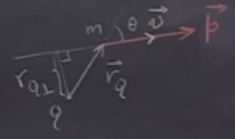
\includegraphics[scale=0.7]{Graphics/lec20_angular_momentum}
\end{center}

The definition is then that the angular momentum relative to the point Q is

\begin{equation}
\vec{L_Q} = \vec{r_Q} \times \vec{p} = (\vec{r_Q} \times \vec{v}) m
\end{equation}

The direction can be found via the right-hand rule (into the blackboard in this case), and the magnitude is

\begin{equation}
|L_Q| = m v r_Q \sin \theta
\end{equation}

where, in shorthand notation, $r_Q \sin \theta = r_{\perp Q}$ may also be used. $\theta$ is, as usual in these cases, the smallest angle between the two vectors. This magnitude follows directly from the definition of the cross product, $\vec{a} \times \vec{b} = a b \sin \theta$. Also, $m(\vec{a} \times \vec{b}) = m a b \sin \theta$; nothing strange there.

Things do start to get strange now, however. We can consider the angular momentum as seen from a different point, call it C, that is located anywhere along the line of the velocity vector (i.e. a point where the object has been, or will be, assuming the direction of the velocity does not change).\\
Here, because $\vec{r_{C}} \times \vec{v} = \vec{0}$, since the two are parallel and cross products have a $\sin \theta$ term in them, the angular momentum relative to C is zero.\\
If we instead choose a point D above this line, the angular momentum relative to this new point D even has the opposite direction as the angular momentum relative to point Q.

This is then clearly a major difference between angular momentum and ``regular'' momentum (linear momentum, or translational momentum; both names are used).\\
Linear momentum has a certain value that is fixed for a certain reference frame. (We can still find reference frames where it is zero, or even opposite in direction, but that is a different discussion.)\\
Angular momentum, however, depends not only on your reference frame, but also on your point of origin. If you consider the origin to be at yourself, and look at a moving object, its angular momentum depends on where you stand, not only on your reference frame.

Consider the case of an object moving along a parabola (or a similar shape -- with or without air drag). It starts out at a point C, and first moves up, and then falls back down, all the while it moves at constant velocity along the x axis.

At time $t = 0$, the object is located at point C, so the angular momentum at time $t = 0$ is clearly 0: $\vec{r_C} = 0$ makes the cross product zero.\\
At any later time, however, there is a nonzero position vector, and a velocity vector that is not parallel to the position vector. Therefore, angular momentum is constantly changing. This does make sense, since the velocity vector is constantly changing.

There are, however, cases where a constantly changing velocity does not imply that angular momentum is changing.

Consider the Earth, going around the Sun, in a circular orbit. (The true orbit is elliptical, but we have not introduced such orbits yet.)

We define the point C to be at the center of the orbit, i.e. at the center of the Sun. We then have the position vector $\vec{r_C}$ to the Earth, which itself has a velocity vector $\vec{v}$, which is always changing, to be tangential to the orbit. The orbital speed $v$ is constant, however.

\begin{center}
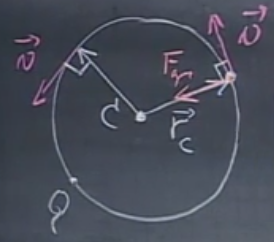
\includegraphics[scale=0.7]{Graphics/lec20_orbit_torque}
\end{center}

The direction of the angular momentum relative to point C, $L_C$, is easy to find via the right hand rule; it is out of the page. The magnitude is found as

\begin{equation}
|L_C| = m v r_C \sin \theta
\end{equation}

However, the angle $\theta$ between the position vector and the Earth's velocity vector is always 90 degrees. Therefore, the sine of that angle is always 1, and $|L_C| = m v r_C$.\\
A while later in time, the exact same thing still applies. The velocity vector has changed direcion, but the direction of the cross product remains constant. $\theta$ remains 90 degrees, and so the magnitude remains.\\
The angular momentum, relative to point C, is constant.

What about relative to some other point $Q$, which is on the Earth's orbital circle? It is clearly changing with time. When the Earth is \emph{at} that point, it must be zero, since $r_Q = 0$. When the Earth is \emph{not} at that point, it must be nonzero, as $\vec{r_Q} \times \vec{v} \neq 0$.

In other words, angular momentum is \emph{conserved} relative to point C, but is \emph{not} conserved relative to any other point!

\subsection{Torque}

Let's now have a look at torque. If angular momentum is the rotational analogue of linear momentum, torque is the rotational analogue of force.

We can write down an expression for the angular momentum relative to some point Q (which can be any point whatsoever), and then take the time derivative of that expression. We will need to use the product rule, though that is not a particularly difficult task:

\begin{align}
\vec{L_Q} &= \vec{r_Q} \times \vec{p}\\
\frac{dL_Q}{dt} &= \frac{d\vec{r_Q}}{dt} \times \vec{p} + \vec{r_Q} \times \frac{d\vec{p}}{dt}
\end{align}

The first of the two terms is the cross product between $\vec{v_Q}$ and the momentum vector of the Earth, but because that velocity and the momentum vector are always parallel ($\vec{p} = m \vec{v}$), that term is zero. What remains is a term that is the position vector cross the net force on the Earth, since $\displaystyle \vec{F} = \frac{d\vec{p}}{dt}$.

The quantity $\displaystyle \frac{d\vec{L_Q}}{dt}$ is known as the \emph{torque} relative to point Q. We use the symbol $\tau$ (greek letter tau) for torque:

\begin{equation}
\vec{\tau_Q} = \frac{d\vec{L_Q}}{dt} = \vec{r_Q} \times \vec{F}
\end{equation}

Torque is also known as moment or moment of force, and may also be translated to something along the lines of ``turning moment'' in some other languages. $M$ or $N$ are other symbols used for torque, especially when it is called moment.\\
Note that torque, exactly as with angular momentum, is also relative to a point! We cannot, in general, talk about ``the'' torque on an object, without specifying our point of origin. Therefore, I used $\vec{\tau_Q}$ above, to show that we are talking about the torque relative to that same point Q.

The torque is the amount of ``twisting'' a force provides. Consider a nut and a wrench. The further out you grip the wrench, the easier it is to loosen a nut/bolt. That is because you are increasing the position vector $\vec{r_C}$, and the torque is proportional to this length. Needless to say, if you increase the amount of force you exert, the torque also increases.

The torque is also proportional to $\sin \theta$ (because of that term in the cross product $\vec{r} \times {F}$) which is quite intuitive. Only the force that is perpendicular to the wrench causes any turning of the nut. If the force is entirely parallel, you are just pushing or pulling on it the nut/bolt, and it will certainly not turn because of that force. For angles in between the extremes of 0 and 90 degrees, the closer you are to a perpendicular angle, the stronger the torque is.

If there is a net torque on an object (relative to a point), angular momentum (relative to that same point) must change. With zero net torque, angular momentum is conserved.\\
There is a clear parallel to conservation of linear momentum here: if there is a net force on an object, its momentum must change. With no net force, momentum is conserved.

Now, consider the case of the Earth orbiting the Sun again. The force vector is always inwards, and it is therefore always antiparallel to $\vec{r_C}$. The cross product $\vec{\tau_C} = \vec{r_C} \times \vec{F}$ is always zero! This is the same result as we found earlier, but now we know why that must be.

Of course, if we calculate the torque at point $Q$, or any other point for that matter, the torque will not be zero, and will also not be constant. We will come back to what is so special about this center point $C$.

\subsection{Spin angular momentum}

So far, we have only really talked about the angular momentum of a point mass, moving through space (even if one such ``point mass'' was the Earth!). We will now consider objects of nonzero size, that rotate around their center of mass. For example, a rotating disk. It has a radius $R$, a mass $M$, and rotates about point C which is its center of mass.

\begin{center}
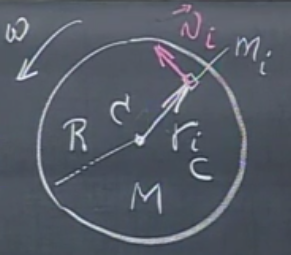
\includegraphics[scale=0.7]{Graphics/lec20_spin_angular_momentum}
\end{center}

We can now, as we did for the moment of inertia among other things, split the disk up into small mass elements $m_i$. Each such element moves with velocity $v_i$. However, as before, we want to express this velocity in terms of $\omega$, since the velocity is a function of the distance to the center, whereas $\omega$ is not. We can use $v_i = \omega r_{iC}$; clearly we need to have that radius in there, anyhow.

The magnitude of the angular momentum for this tiny mass element alone is $L_{Ci} = (\vec{r_iC} \times \vec{v_i}) m_i = m_i r_{iC} v_i = m_i r_{iC}^2 \omega$. There is no $\sin \theta$ term since $\theta$ is always 90 degrees, and so $\sin \theta = 1$.\\
The direction can be found by the right-hand rule as usual, and is out of the blackboard (or page) in this case.

Now, in order to find the total angular momentum, we must sum up the angular momenta of all these tiny mass elements:

\begin{equation}
L_{disk_C} = \sum_i m_i r_{iC}^2 \omega = \omega \sum_i m_i r_{iC}^2 = I_C \omega
\end{equation}

If we factor out $\omega$ of the sum, since it is common to all elements, all that remains in the sum is $\sum_i m_i r_{iC}^2$, which as we have seen previously is just the moment of inertia for the disk. Therefore, we can find the angular momentum of the disk relative to point C as $I_C \omega$.

What is now remarkable is that this value is the angular momentum relative to \emph{all} points anywhere in space, not just relative to point C. This is true because of, and only in the cases where, this is a rotation around the center of mass.

$I_C \omega$ is referred to as the spin angular momentum, and is an intrinsic property of an object, regardless the origin you choose.\\
It is valid for objects of all shape, not only disks, as long as the rotation is about the center of mass.
(Everything I find about the term ``spin angular momentum'' is about quantum mechanics, however. I'm unsure whether this is a common terminology or not, but it appears not.)

$I_C \omega$ for the disk then gives us $\displaystyle L_{disk_C} = \frac{\omega}{2} M R^2$.

This concept is of course very handy. In the case of an object spinning around its center of mass, we can now talk about \emph{the} angular momentum of that disk, without having to specify any point of origin.

The Earth has both a spin angular momentum and an orbital angular momentum due to its motion around the Sun. The spin angular momentum is quite easy to find as $I_C \omega$.\\
The moment of inertia for a sphere spinning about its center of mass is $\displaystyle \frac{2}{5} M R^2$, derived in the previous lecture. Using $R_{Earth} = 6400$ km and $T = 86400$, which translates into $\omega \approx \SI{7.2722e-5}{rad/s}$, 

The spin angular momentum of the Earth is then

\begin{equation}
\left(\frac{2}{5} (\SI{5.972e24}{kg}) (\SI{6400e3}{m})^2\right) (\SI{7.2722e-5}{rad/s}) = \SI{7.11e33}{kg m^2 s^{-1}}
\end{equation}

I'm not sure what units to use; the dimension is $\text{kg m}^2 \text{ s}^{-1}$, which is equivalent to $\text{N}\cdot\text{m} \cdot \text{s}$ and $\text{J} \cdot \text{s}$. Presumably one set of units is more common than the others!\\
... Coming back to this section after having finished this week's lectures, I would guess that the newton-meter-second is the most common unit (in general) for angular momentum. If a torque of 1 Nm acts for 1 second, the angular impulse (the change in angular momentum) is (1 Nm)(1 s) = 1 Nms. In this particular case (above), though, we have the units explicitly in terms of kg, $\text{m}^2$ and rad/s.

Anyhow.
The orbital angular momentum around the Sun, relative to the center of the orbit, is

\begin{equation}
L_C = (|\vec{r_C} \times \vec{v}|) m = m r_s \frac{2 \pi r_s}{T_{orbit}} = \frac{2 \pi m r_s^2}{T_{orbit}}
\end{equation}

where $r_s$ is the radius of the Earth's orbit, about 150 million km, or \SI{1.5e11}{m}. The mass $m$ is $\SI{5.97e24}{kg}$. $T_{orbit} \approx 86400 \times 365$, so
This then gives us \SI{2.677e40}{kg m^2 s^{-1}}.

The ratio of the two, with spin angular momentum on top, is about $\num{2.66e-7}$.

\subsection{Conservation of angular momentum: an experiment}

Consider a person, standing on a plate that is free to rotate, like this:

\begin{center}
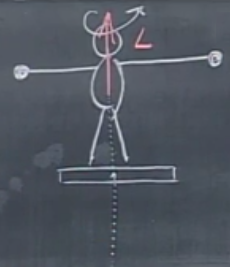
\includegraphics[scale=0.7]{Graphics/lec20_cons_angular_momentum}
\end{center}

In his hands, he holds two weight of mass $m \approx 1.8$ kg (each). The mass of the person, including the weights plus the turntable itself, is $M \approx 75$ kg.
In this counterclockwise rotation, seen from above (clockwise from below, though I find it easier to see this from above), the angular momentum vector will be upwards.

In a case like this, we have a rotation about a center of mass. Angular momentum has a value found simply by $I_C \omega$, and it will be conserved, after the initial push to get the person rotating. When rotating, these weights can be moved either close to his body, or as far out as his arms can reach. Clearly, this does not cause an \emph{external} torque, so angular momentum $L_C$ must be conserved.

However, $I_C$, the moment of inertia, will change! Since $L = I_C \omega$, and $I_C$ will go down, $\omega$ must go up -- there is no other way for the conservation to hold.

In a semi-quantitative calculation, we can approximate the professor as a cylinder, with radius $R = 0.2$ m. The cylinder has a mass of 75 kg\footnote{I think it should be 75 kg minus the 2 times 1.8 kg, but these numbers will clearly not be very accurate either way.}, and so has a moment of inertia of about $\frac{1}{2} M R^2 = \SI{1.5}{kg m^2}$.

Now, if we ignore the weight of the professor's arms, when stretching them out, two additional point masses are added, at arm's length from the axis of rotation. The moment of inertia for each weight is about $m r^2 = \SI{1.5}{kg m^2}$, assuming an arm length of 90 cm.\\
When his arms are stretched out, we then find the total moment of inertia to be the roughly 1.5 from the professor's body, plus another 3 from the weights! This difference of a factor of 3 (4.5/1.5) when pulling the weight in close causes a difference in $\omega$ of a factor of three, so the change in the angular velocity is very apparent!

\subsection{Conservation of angular momentum (in general, and in stars)}

Let's look at conservation of angular momentum in a similar way to how we treated linear momentum.

Say we have a group of objects interacting: stars, interacting gravitationally, point particles of any kind, objects connected together with springs, etc. There can be any kind of internal interactions between these, including collisions, internal friction, explosions/supernovae, and so on.\\
Because all internal forces will cancel out, there can never be any net internal torque relative to any point Q we choose. In the absensce of a net \emph{external} torque, angular momentum will be conserved. In the prescence of a net external torque, angular momentum will change according to

\begin{equation}
\frac{d\vec{L_Q}}{dt} = \vec{r_Q} \times \vec{F_{Ext}} = \vec{\tau_{Q,Ext}}
\end{equation}

... for the entire system as a whole. The angular moment of any one object \emph{inside} that system is, just as with linear momentum, \emph{not} conserved. Essentially, they can ``trade'' angular momentum with each other, but the net angular momnetum of the entire system cannot change.

Similar to the experiment the professor did, reminiscent of ice skaters, stars can also shrink, and have their moments of inerta go down (since $I \propto R^2$), which means that the star's angular velocity must increase: $L = I \omega$ must be constant in the absence of a net external torque.

In a star, 	the nuclear fusion going on causes forces that want to expand the star outwards. However, there is also gravity, which does what it can to collapse the star towards its center. In all stars that are actively ``burning'' fuel, these two forces are balanced out.

What now happens when the fuel runs out, and fusion can't continue on? This won't happen for about 5 billion years for our Sun, but it happens all the time for other stars, considering the amount of stars in the observable universe. There are three possible end products of stars.

The first is that the star becomes a \emph{white dwarf}. They have radii of about $10^4$ km, not too far from the radius of the Earth, and a mass of about half our Sun's mass. Our Sun will end up as a white dwarf far in the future.\\
We can see that the density of such an object must be very high, with half the Sun's mass, but a volume almost comparable with that of the Earth. The density becomes on the order of $\SI{1e6}{g/cm^3}$.

The second possibility is that the star becomes a \emph{neutron star}, a very interesting type of celestial object. They have radii on the order of 10 kilometers -- less than many cities -- yet a mass typically in the range 1.4 to 3.2 solar masses! This causes a ridiculous density of some $10^{14} \text{ g/cm}^3$. Neutron stars are so named because they are thought to consist largely of neutrons. In some ways, they are like enormous nuclei.\\
The Crab pulsar, which we discussed earlier, is a neutron star. In fact, all pulsars are neutron stars. Not all neutron stars are pulsars, however, since they do stop rotating sooner or later, at which point they no longer pulse. Also, pulsars are mostly defined by the fact that they pulse towards the Earth, so the vast majority of such neutron stars may go unnoticed, since their light beams are unlikely to be pointed towards us.

Finally, the third possibility is that the star becomes a \emph{black hole}, an even more bizarre type of celestial object. This can only happen for stars that are more massive than about three solar masses.\\
Black holes will not be covered in this lecture, but will be in the future.

When a star collapses, due to the lack of outwards pressure, a huge amount of gravitational potential energy is converted to kinetic energy, as the mass of the star falls inward. That energy is ultimately turned into heat and radiation.\\
In addition, because the moment of inertia is reduced as the mass moves inwards, the rotational period of the star increases, often dramatically. (Especially for neutron stars, see below.)

Our Sun will not become a neutron star, as it is not massive enough, but let's do some calculations on it anyway, just to get a feeling for some numbers. The radius of the Sun is about 700 000 km, while that of a neutron star might be about 10 km.\\
The mass is about $\SI{2e30}{kg}$. In moving all this mass inwards, there is a huge loss in gravitational potential energy, on the order of $\Delta U = 10^{46}$ joules.\\
This is converted to kinetic energy, and then converved into heat and radiation, etc.

This energy is on the order of \emph{100 times more} than the Sun releases in its \emph{10 billion year} lifetime -- and this explosion releases that energy in a matter of seconds, rather than billions of years! This is what we call a supernova. (There are different types of supernovae; this is one of them.)

``A white dwarf, with a mass of $\SI{2.8e30}{kg}$ and a radius of about 10 000 km implodes (via gravitational collapse) to becomes a neutron star of the same mass with a radius of about 10 km. The rotational period of the white dwarf was $T_i = 10$ hours. What will the rotational period of the neutron star be? For simplicity, assume that the mass density in both the white dwarf and the neutron star is uniform.''

Okay, so let's first convert these numbers a little. The initial radius is $10000\times10^3 = 10^7$ m, and the final radius $10^4$ m. The initial period is $T_i = 36000$ seconds.

$\displaystyle L = I \omega = I \frac{2 \pi}{T}$ is conserved, so when $I$ goes down, $T$ must go down by the same factor. $I \propto R^2$, and the change in $R$ is a factor $10^3$, so the change in $R^2$ in a factor of $10^6$. The time period becomes $T = 36000 \times 10^{-6} = 0.036$ seconds (27.77 Hz, up from $\SI{2.77e-5}{Hz}$!).

\subsection{More on supernovae, pulsars and neutron stars}

The idea behind these notes is not to provide a transscript, and as such, as I do now and then, I recommend simply watching this part of the lecture at this point. There is quite a bit of information, but most of it works better in context in the video, so I see little point in copying it down here almost verbatim!

\section{Lecture 21: Torque}

The lecture begins with a review of the last week. I didn't find anything in particular to take notes of again. After all, being able to review is sort of the point of these notes!

Still, here are a few equations given:

\begin{align}
\vec{L_Q} &= \vec{r_Q} \times \vec{p}\\
\vec{\tau_Q} &= \vec{r_Q} \times \vec{F}\\
\frac{d\vec{L_Q}}{dt} &= \vec{\tau_{Q,Ext}}
\end{align}

The last equation is often used for a system of objects, thus the ``external'' qualifier. With no net \emph{external} torque, angular momentum in conserved... relative to that point Q, since that may be the only point with zero torque.

In rotation about some point Q, we can write a variant of Newton's second law, that relates torque with moment of inertia and angular acceleration (rather than relating force with mass and linear acceleration), as well as a relation that relates angular momentum with moment of inertia and angular velocity (rather than relating linear momentum with mass and linear velocity):

\begin{align}
|\tau_Q| &= I_Q\ \alpha_Q \text{, where $\alpha = \ddot{\theta}$, $\omega_Q = \dot{\theta}$}\\
|L_Q|    &= I_Q\ \omega_Q
\end{align}

In the special case of a rotation about the center of mass of an object, the angular momentum is instead an intrinsic property of that object, and it \emph{no longer matters} which point Q we choose. In that case

\begin{equation}
|L_{cm}| = I_{cm} \omega_{cm}
\end{equation}

In all other cases, it is crucial to specify the point of origin chosen, since angular momentum depends on not only your reference frame, but also the point of origin.

Let's now look at a case where angular momentum is conserved for exactly one point, but is not conserved for any other.\\
We have a rod, that we rotate about a point P, which is a distance $d$ from the center of mass C. It has a mass $M$ and a length $\ell$, and we rotate it with an angular velocity $\omega$.

\begin{center}
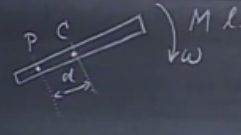
\includegraphics[scale=0.7]{Graphics/lec21_rod}
\end{center}

The moment of inertia for rotation about the center of axis of a rod of uniform density is $\displaystyle \frac{1}{12} M \ell^2$, so angular momentum relative to point P is

\begin{equation}
|L_P| = I_P \omega = \left(\frac{1}{12} M \ell^2 + M d^2\right) \omega
\end{equation}

where the $M d^2$ term is added because of the parallel axis theorem.

There will be a force acting on the ruler at point P, as well as one acting on the pin (that it rotates around) \emph{by} the ruler. We can show this by analogy. Consider a massless rod, with two equal masses on each end. We rotate this rod about the center of mass, which is also the center of the rod. There is a centripetal force inwards on each of the masses, of equal magnitude since the masses are equal and the distance from the point of rotation are equal (and the velocities of the masses are then also equal).\\
However, if we rotate the rod about a point that is closer to one of the masses, then the centripetal force on that mass is smaller, but the centripetal force no the other is larger, since they move in circles of different radius. (As the point of rotations comes closer to one of the masses, it almost doesn't rotate at all, but rather spins about its axis.)

For this reason, there will be a force on the pin (and a reaction force from it) at point P in the ruler. The \emph{torque} relative to point P is zero, however: the force is along the ruler, and the position vector in $\vec{r} \times \vec{F}$ is also along the ruler.

Since $|\vec{\tau_P}| = 0$, angular momentum is conserved in this case. It would not be if we chose any other \emph{stationary} point, however.

Let's now rotate the same ruler about the center of mass C. The problem is now symmetric, like the case with the two masses mentioned above, and so there is now no net force on the pin/due to the pin. With no net force, $\vec{\tau_Q} = \vec{r_Q} \times \vec{F}$ must be zero for \emph{all} points Q, since $F = 0$. Therefore, in this case, angular momentum is conserved relative to \emph{all} points, as there is no net torque relative to \emph{any} point. The magnitude of the angular momentum for the rotation about the center of mass is then simply $I_C \omega$, which for a rod is

\begin{equation}
|L_{CM}| = \frac{1}{2} M \ell^2 \omega
\end{equation}

for all points in space.

\subsection{Off-center impulse: translation and rotation}

Let's now consider a ruler, lying flat on a frictionless table. It has a uniform mass density, and so its center of mass C is located at the geometric center. We give it an impulse $I$, in other words, a force that acts for a certain amount of time (a very short amount of time in this case, but that is not strictly necessary for this to hold).

\begin{center}
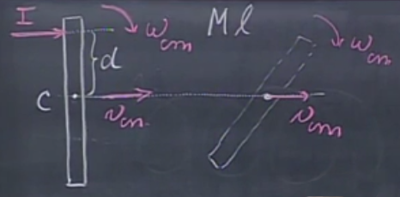
\includegraphics[scale=0.7]{Graphics/lec21_ruler_rotation}
\end{center}

What will happen? Clearly, it is going to move towards the right. It will also rotate, assuming you don't aim for the center of mass (i.e. assuming $d \neq 0$).

The object \emph{must} rotate about its center of mass -- anything else is impossible. If it were to rotate about a point offset from the center of mass, then the center of mass would have to move in a spiral-ish motion. Due to conservation of (linear) momentum, the center of mass must have a constant velocity (meaning both magnitude and direction are constant!) after the initial push, which is only possible if any rotation is about the center of mass.\\
(Keep in mind that this is assuming a frictionless table. On a real table, where $\mu$ likely differs at different points, the results may also therefore differ: there is then an external force that may vary in unpredictable ways!)

That much is fairly intuitive, in my opinion, but what's interesting that the distance $d$ from the center of mass where the impulse happens does not affect the velocity of the center of mass. For a given amount of momentum given by the impulse, the velocity of the center of mass is constant, regardless of $d$. I find this nonintuitive, but it is still easy to see mathematically.

$\vec{p} = m \vec{v_{cm}}$ must hold, and since initial momentum is 0, $\vec{p} = \vec{I}$ after the initial push. Nowhere in the equation does $d$ appear -- the equation in question is valid for any isolated system, regardless of shape and place where the force is applied, as long as it is rigid.\\
Since $\vec{p} = \vec{I}$, the above equation also says that

\begin{equation}
\vec{v_{cm}} = \frac{\vec{I}}{m}
\end{equation}

$\omega$, on the other hand, clearly depends on the distance $d$. If $d = 0$, then $\omega = 0$; that much is clear. It is also clear that $\omega$ grows as $d$ grows. The reason is that the amount of torque (relative to the center of mass) provided depends on $d$ and the amount of force provided during the impulse. (The amount of angular impulse, i.e. change in angular momentum, depends on the average torque and the time, $J = \tau \Delta t$, just like how the linear impulse is given by $I = F \Delta t$.)\\
($\omega$ was calculated in this week's homework: week 9/homework 7, problem 9.)

However, note that if we instead look at the torque relative to a point P on the line of the impulse, i.e. a distance $d$ up from the center of mass, this torque is zero! Zero torque means angular momentum will be conserved, and so angular momentum \emph{relative to point P} is zero not only before, but also after the object starts to rotate. It is therefore conserved, unlike angular momentum relative to the center of mass!

\subsection{Physical pendulum}

Let's have a look at a different ruler. We previously derived an equation describing the motion of a simple pendulum, as a simple harmonic oscillator. We made some unrealistic approximations, however, including a massless string and a point mass hanging from it.\\
We will now consider a related yet different type of oscillator, called a physical pendulum.

In this case, we have a ruler, though the solution is valid for other shapes as well. We drill a hole through it at point P, and hang it on a small pin. The point P is located a distance $b$ from the center of mass, point C.

\begin{center}
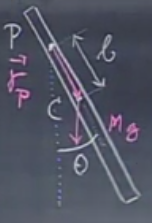
\includegraphics[scale=0.7]{Graphics/lec21_physical_pendulum}
\end{center}

The ruler makes an angle $\theta$ with the vertical. Using the concept of the center of mass, we can consider gravity acting only at the center of mass; the magnitude is $M g$, where $M$ is the total mass of the ruler.

If we choose to use point P as our origin, our lives become much easier. There will be a force at point P, but if we choose it as our origin, we do not have to worry about those forces, since the torque due to those forces will be zero: $\vec{\tau_P} = \vec{0} \times \vec{F}$, since the first term is the position vector from P to P.

There is a torque that matters, relative to point P, however: the torque due to gravity acting on the center of mass. The distance $b$ acts as a lever arm, and the torque is given as the cross product between the distance and the force. The torque can also be found as $I_P \alpha$, as we saw earlier.

\begin{equation}
|\vec{\tau_P}| = \vec{b} \times \vec{F_g} = M g b \sin \theta = - I_P \alpha
\end{equation}

The torque is always trying to restore things back to equilibrium, which gives us a minus sign, just as how we used $- k x$ for the force when deriving the equation governing a spring oscillator. Note that we have used the Newton's second law equivalent for torques: $F = m a \Rightarrow \tau = I \alpha$.

$\alpha = \ddot{\theta}$ by definition, in a different form of notation. Now, using the small angle approximation that we have used several times earlier, $\sin \theta \approx \theta$. This is fairly valid for small angles; at 5 degrees, the difference is less than 0.15\%; at 10 degrees, the difference is about 0.5\%.\\
By using this approximation, and making the substitution for $\alpha$, we have

\begin{align}
M g b \theta &= - I_P \ddot{\theta}\\
I_P \ddot{\theta} + M g b \theta &= 0\\
\ddot{\theta} + \frac{M g b}{I_P} \theta &= 0
\end{align}

A-ha! This has the exact form of a simple harmonic oscillator! We already know the solutions; the square root of the stuff multiplying $\theta$ gives us the angular frequency $\omega$, etc:

\begin{align}
\theta(t) &= \theta_{max} \cos(\omega t + \phi)\\
\omega    &= \sqrt{\frac{M g b}{I_P}}\\
T         &= \frac{2 \pi}{\omega} = 2 \pi \sqrt{\frac{I_P}{M g b}}
\end{align}

Keep in mind that because $I_P \propto M$, this is in fact independent on the mass, just as with a simple pendulum. We can substitute in the value for $I_P$, in which case we transform the general result, above, into a result that only holds for a rod.\\
$I_P = \frac{1}{12} M \ell^2 + M b^2$ via the parallel axis theorem. Making that substitution,

\begin{align}
\omega    &= \sqrt{\frac{g b}{\frac{1}{12} \ell^2 + b^2}}\\
T         &= \frac{2 \pi}{\omega} = 2 \pi \sqrt{\frac{\frac{1}{12} \ell^2 + b^2}{g b}}
\end{align}

Again, note that these results are now only valid for the case of a rod.

As a side note, we can also write for the angular acceleration $\alpha = \dot{\omega}$. This is a very confusing thing to do, however! The omega in the previous sentence is the \emph{angular velocity}, i.e. how fast the angle is changing with time, analogous to the velocity $v$ for linear motion. This omega is \emph{constantly changing in time}, and has a minimum at $\theta_{max}$, as the pendulum reverses direction, and a maximum at $\theta = 0$.

On the other hand, the $\omega$ used in the cosine above, and the only one I have mentioned prior to the paragraph above to avoid confusion, is the \emph{angular frequency}, $\displaystyle \omega = \frac{2 \pi}{T}$. That $\omega$ is a \emph{constant}, and is only related to how many oscillations the pendulum completes per second. This sentence marks the last mention of the angular velocity $\omega$ in this section; only the one that represents angular \emph{frequency} will be used from here on.

Let's try to calculate the approximate period, including the uncertainty, of this pendulum when $\ell = 1.00$ m and $b = \SI{0.400(2)}{m}$, i.e. the uncertainty is 2 mm or 0.2 cm.

In the ideal case, the number we find by plugging in the numbers is $T = \SI{1.5497}{s}$, using $g = \SI{10}{m/s^2}$.\\
The largest possible time should be when $\ell$ and $b$ are both maximized, which gives $T = 1.556$ s. On the other side of things, the smallest possible period is about $T = 1.543$ s.

The uncertainty is about 0.0065 seconds or so; call it 0.01 s.\\
It turns out the professor used $g = \SI{9.8}{m/s^2}$, which is probably a good idea if you're going to time this in the real world. In either case, he found $T = 1.565$ seconds, which is very close to these numbers.

This is then demonstrated, and the timing indeed works out.

Next, we look at the same type of oscillation, but we use a hula hoop as the pendulum, instead of the ruler. The derivation is almost identical, and except for some variable names, we can still use the general equation we found earlier.

The center of mass of the hoop is at the geometric center, i.e. in the middle of empty space. We again hang it on a pin, at point P, which clearly is at the very top of the hoop.

\begin{center}
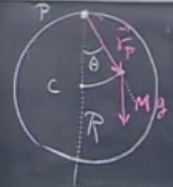
\includegraphics[scale=0.7]{Graphics/lec21_hoop_pendulum}
\end{center}

As before, we consider the force of gravity as acting solely on the center of mass, with a force $M g$ downwards. Again as before, the position vector $\vec{r_P}$ acts as the lever arm, and the torque relative to point P is

\begin{equation}
\vec{r_P} \times \vec{F_g} = M g R \sin \theta = -I_P \ddot{\theta}
\end{equation}

As before, the torque must be equal to the negative of $I_P \alpha = I_P \ddot{\theta}$, using Newton's second law for circular motion. If we use the small angle approximation $\sin \theta \approx \theta$ again, and solve for $\ddot{\theta}$:

\begin{equation}
\ddot{\theta} + \frac{M g R}{I_P} \theta = 0
\end{equation}

Clearly, this is yet another simple harmonic oscillator! The only difference from the one we found for the rod is that we now used $R$ instead of $b$ for the distance to the center of mass; they are identical other than that non-detail.\\
The moment of inertia about point $I_P$ is the moment inertia about the center of mass $I_C$, plus $M R^2$ via the parallel axis theorem. $I_C$ is also $M R^2$ for a circular object with uniform mass distribution (all mass points are a distance $R$ away (derivation not shown), so $I_P = 2 M R^2$. That gives, using the solutions we found previously and using this new $I_P$,

\begin{align}
\theta(t) &= \theta_{max} \cos(\omega t + \phi)\\
\omega    &= \sqrt{\frac{g}{2 R}}\\
T         &= \frac{2 \pi}{\omega} = 2 \pi \sqrt{\frac{2 R}{g}}
\end{align}

This is the same result as we have found previously for a pendulum with a massless string, if we just call its length $2 R$! Quite neat, that they would have the same period.	

Time for an interesting lecture question.

\begin{center}
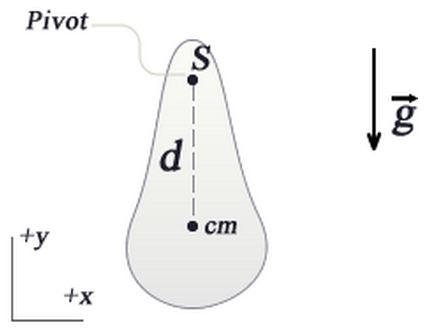
\includegraphics[scale=0.5]{Graphics/lec21_physical_pendulum_2}
\end{center}

``A physical pendulum consists of a body of mass m contained in the xy-plane. The moment of inertia of the object about an axis perpendicular to the plane and passing through the object's center of mass is Icm.

The object oscillates in the xy-plane about the point S a distance $d$ from the center of mass as shown. What is the period of the pendulum for small angle oscillations where $\sin\theta \approx \theta$?''

Since they want the answer in terms of $I_{cm}$ (so that we don't need to actually calculate the moment of inertia) this should be fairly easy. In fact, we just use the general solution with $d$ as the distance between the point and the center of mass,

\begin{equation}
T = 2 \pi \sqrt{\frac{I_{S}}{m g d}}
\end{equation}

$I_S$ can be written as $I_{cm} + m d^2$, so

\begin{equation}
T = 2 \pi \sqrt{\frac{I_{cm} + m d^2}{m g d}} = 2 \pi \sqrt{\frac{I_{cm}}{m g d} + \frac{d}{g}}
\end{equation}

There is then a demonstration of the hula hoop, and a simple pendulum (an apple hanging on a lightweight string), to show that their periods are almost synchronized. (Most of the error likely comes from a small difference in length.)




























\part{Homework problems}

\setcounter{chapter}{0}

\chapter{Week 1: Homework 1}

\section{Problem 1: Decomposing vectors}

``Consider two vectors in the xy-plane as shown.

\begin{center}
\includegraphics[scale=0.8]{Graphics/h1p1}
\end{center}

Vector $\vec{A}$, in the first quadrant, has a magnitude $|\vec{A}| = 2.0$ and is at an angle $\alpha = \ang{40}$ with respect to the positive x-axis. Vector $\vec{B}$, in the fourth quadrant, has a magnitude $|\vec{B}| = 1.5$ and is at an angle $\beta = \ang{20.0}$ with respect to the positive x-axis.

Find the x and y components of the vectors $\vec{A}$ and $\vec{B}$.''

Well, this ought to be fairly simple. First, let's consider what sort of values we expect. $\alpha$ is in the first quadrant that is, angled upwards and to the right. That means $A_x > 0$ and $A_y > 0$.\\
We could use the formulas listed in the first part of these notes, or simply re-derive them from the basic trig definitions. I prefer the latter route, since it can be done in a few seconds once you're comfortable with it, and it means you can't remember them the wrong way. (Unless you misremember everything central to trigonometry!)

$A_x$ is the adjacent side to $\alpha$, while $\vec{A}$ is the hypotenuse, and $A_y$ is the opposite. Using trig definitions, we find

\begin{equation}
\sin \alpha = \frac{A_y}{|\vec{A}|}
\end{equation}
\begin{equation}
A_y = |\vec{A}| \sin \alpha
\end{equation}

\begin{equation}
\cos \alpha = \frac{A_x}{|\vec{A}|}
\end{equation}
\begin{equation}
A_x = |\vec{A}| \cos \alpha
\end{equation}

The same relations hold for $\beta$ and $\vec{B}$ as well, of course, so we just need to enter these answers into the form (and convert the degree values to radians inside the trig functions), and we're done!

\section{Problem 2: Catching up}

``During a track event two runners, Mary, and Alice, round the last turn and head into the final stretch with Mary a distance $d = 3.0$ m in front of Alice. They are both running with the same speed of $v_0 = 7.0$ m/s. When the finish line is a distance $L = 45.0$ m away from Alice, Alice accelerates at $a_A = 1.5\text{ m/s}^2$ until she catches up to Mary. Alice then continues at a constant speed until she reaches the finish line.

\begin{center}
\includegraphics[scale=0.8]{Graphics/h1p2}
\end{center}

(a) How long (in s) did it take Alice to catch up with Mary?''

First up, we need to choose a reference frame to work in. I considered choosing Mary's refrence frame, so that she is seen as stationary, but that would probably just cause problems in some aspects of the problem.\\
I'll therefore choose the simple one, where the track and the finish line are stationary.

Since there are five sub-question, let's set up some equations. We know the initial position of each runner (we'll call Alice's position 0, and therefore Mary's initial position is $d$), initial velocity, and acceleration.

For Alice:
\begin{align}
x_A(t) = v_0 t + \frac{3}{4} t^2\\
v_A(t) = v_0 + 1.5 t
\end{align}
(Alice's acceleration is due to the \SI{1.5}{m/s^2} times the one-half present in the formula.)

And for Mary:
\begin{align}
x_M(t) &= d + v_0 t\\
v_M(t) &= v_0
\end{align}

So, let's restate the question:
``(a) How long (in s) did it take Alice to catch up with Mary?''

We set their position equations equal, and solve for $t$:

\begin{align}
\frac{3}{4} t^2 = d\\
t^2 = \frac{4}{3} d\\
t = +\sqrt{\frac{4d}{3}} = \SI{2}{s}
\end{align}

``(b) How far (in m) did Alice still have to run when she just caught up to Mary?''

It took 2 seconds exactly, so Mary must have moved 14 meters (2 seconds, 7 m/s) in that time, to position $d + \SI{14}{m}$.\\
The distance remaining is $L - d - \SI{14}{m} = \SI{28}{m}$.

``(c) How long (in s) did Alice take to reach the finish line after she just caught up to Mary?''

Keep in mind that she stopped accelerating when she passed, so her velocity is now a constant again. She started out at 7 m/s and accelerated at \SI{1.5}{m/s^2} for 2 seconds, so her velocity is now \SI{10}{m/s}. The answer is the distance remaining divided by her velocity, so the answer is

\begin{equation}
\text{time taken} = \frac{L - d - \SI{14}{m}}{\SI{10}{m/s}} = \SI{2.8}{s}
\end{equation}

``Mary starts to accelerate when Alice just catches up to her, and accelerates all the way to the finish line and crosses the line exactly when Alice does. Assume Mary's acceleration is constant.\\
(d) What is Mary's acceleration (in $\text{m/s}^2$)?''

To sum up where we're at: Mary is still running at 7 m/s, with 28 meters left to go. Alice is running at 10 m/s, also with 28 meters left to go (meaning she will get there in 2.8 seconds).\\
Mary must now accelerate such that $x_M(t) = L$ at $t = \SI{2.8}{s}$ (we reset the current time to $t=0$ for simplicity).

Mary's new position equation is

\begin{equation}
x_M(t) = (L - \SI{28}{m}) + v_0 t + \frac{1}{2} a t^2
\end{equation}

We need that it to be equal to $L$ at $t = \SI{2.8}{s}$ as mentioned, so we substitute the values for $t = \SI{2.8}{s}$ and $v_0 = \SI{7}{m/s}$ in, set it equal, and solve for $a$:

\begin{align}
(L - \SI{28}{m}) + (\SI{7}{m/s})(\SI{2.8}{s}) + \frac{1}{2}\ a\ (\SI{2.8}{s})^2 = L\\
- \SI{28}{m} + \SI{19.6}{m} + \SI{3.92}{s^2} \cdot a = 0\\
\SI{3.92}{s^2} \cdot a = \SI{28}{m} - \SI{19.6}{m}\\
a = \frac{\SI{28}{m} - \SI{19.6}{m}}{\SI{3.92}{s^2}} \approx \SI{2.14}{m/s^2}
\end{align}

``(e) What is Mary's velocity at the finish line (in m/s)?''

That would be given by her old velocity, 7 m/s, plus the acceleration multiplied by the time accelerated (2.8 seconds):

\begin{equation}
v_{M_{final}} = \SI{7}{m/s} + \SI{2.14}{m/s^2} \cdot \SI{2.8}{s} \approx \SI{13}{m/s}
\end{equation}

\section{Problem 3: Speeding ticket}

This problem was removed from the grading, i.e. assigned 0 points, after there had been some trouble with it. The problem is supposed to be fixed now, however, so I will attempt it.

``A motorist traveling with constant speed of $v_c = 18.0$ m/s passes a school-crossing corner, where the speed limit is 10 m/s. Just as the motorist passes, a police officer on a motorcycle stopped at the corner starts off in pursuit. The officer accelerates from rest at $a_m = \SI{3.00}{m/s^2}$ until reaching a speed of 30.0 m/s. The officer then slows down at a constant rate until coming alongside the car at x = 270.0 m.\\
Consider a coordinate system with origin at the school-crossing corner, $x = 0$, and the +x-axis in the direction of the car's motion.

(a) How long does it take for the motorcycle to catch up with the car (in s)?''

Okay. The car moves at a constant velocity, so that part is easy. Now, as for the offices, he takes 10 seconds to accelerate to his top speed. During that time, his new position is

\begin{align}
x_m(t=10) &= x_0 + v_0 t + \frac{1}{2} a t^2 = \frac{1}{2} (\SI{3}{m/s^2}) (\SI{10}{s})^2\\
          &= \SI{150}{m} \text{ (answers question c)}
\end{align}

As mentioned above, this also  answers part (c): ``(c) How far (in m) is the motorcycle from the corner when switching from speeding up to slowing down?''

In fact, I think the next question that should be answered is (d), not (a), so let's see.

``(d) How far (in m) is the motorcycle from the car when switching from speeding up to slowing down?''

We don't really need to write down the position equation here, as it's a bit too simple: $x = \SI{18.0}{m/s} \cdot \SI{10}{s} = \SI{180}{m}$. Since the motorcycle is 150 m from the corner, the answer here must be 30 m.

So, we are now at: motorist at $x = 180$ m at 18.0 m/s, cop at $x = 150$ m at 30.0 m/s. The cop must slow down with constant acceleration so that he hits $x = 270$ m at the same time as the motorist. At the motorists' speed, that happens at

\begin{equation}
t = \SI{10}{s} + \frac{\SI{270}{m} - \SI{180}{m}}{\SI{18.0}{m/s}} = \SI{15}{s}
\end{equation}

... where 10 seconds is the time that has already passed. Alternatively, we could simply take the 270 meters divided by the velocity to find the same result. This answers question (a). Back to (e):

All in all, we set up a new equation for the cop. $x_0 = \SI{150}{m}$, $v_0 = \SI{30.0}{m/s}$, and $a$ is our unknown. The position equation must equal 270 m at $t = \SI{5}{s}$ -- we reset $t$ to start over from the instant where the above parameters are true:

\begin{align}
\SI{150}{m} + (\SI{30.0}{m/s})(\SI{5}{s}) + \frac{1}{2} a (\SI{5}{s})^2 = \SI{270}{m}\\
\frac{1}{2} a (\SI{5}{s})^2 = \SI{-30}{m}\\
a (\SI{25}{s^2}) = \SI{-60}{m}\\
a  = \frac{\SI{-60}{m}}{\SI{25}{s^2}} = \SI{-2.4}{m/s^2}
\end{align}

\section{Problem 4: Position, velocity and acceleration}

``An object is moving along a straight line parallel to the x-axis. Its position as a function of time is given by:\\
$x(t) = \SI{30}{m} - (\SI{21}{m/s}) t + (\SI{3}{m/s^2}) t^2$\\
where the position x is in meters and the time t is in seconds.

(a) What is the object's velocity at $t = 0$ s, 2 s, and 5 s?''

We take the derivative of the above equation, and end up with

\begin{equation}
v(t) = - \SI{21}{m/s} + (\SI{6}{m/s^2}) t
\end{equation}

All we need to do now is plug in the values for $t$.

``(b) What is the object's acceleration at $t = 0$ s, 2 s, and 5 s?''

We take the derivative of $v(t)$ above:

\begin{equation}
a(t) = \SI{6}{m/s^2}
\end{equation}

We don't even need to plug in values here - the answer is $\SI{6}{m/s^2}$ for all three cases.

``(c) At what time T is the object's velocity zero?''

We set $v(t) = 0$ and solve for $t$:

\begin{align}
- \SI{21}{m/s} + (\SI{6}{m/s^2}) t = 0\\
t = \frac{\SI{21}{m/s}}{(\SI{6}{m/s^2})}\\
t = \SI{3.5}{s}
\end{align}

``What is the object's position when its velocity is zero?''

We plug $t = \SI{3.5}{s}$ into $x(t)$ and we're done. Note that the answer (in my case, at least) is negative.

``(d) What is the average velocity between $t_1 = \SI{1.0}{s}$ and $t_2 = \SI{3.5}{s}$?''

With a constant acceleration, as here, we can calculate the average simply by averaging between the velocities at $t_1$ and $t_2$.

\begin{equation}
v_{t_1 t_2 avg} = \frac{v(\SI{1.0}{s}) + v(\SI{3.5}{s})}{2} = \frac{\SI{-15}{m/s} + \SI{0}{m/s}}{2} = \SI{-7.5}{m/s}
\end{equation}

``(e) What is the object's average velocity between $t_1 = \SI{0}{s}$ and $t_2 = \SI{7.0}{s}$?''

Same deal as above.

\begin{equation}
v_{t_1 t_2 avg} = \frac{v(\SI{0}{s}) + v(\SI{7}{s})}{2} = \frac{\SI{-21}{m/s} + \SI{21}{m/s}}{2} = \SI{0}{m/s}
\end{equation}

``(e) What is the object's average speed between $t_1 = \SI{0}{s}$ and $t_2 = \SI{7.0}{s}$?''

Aha! Keep in mind that speed and velocity are \emph{not} the same in physics! Here, because the object has reversed, the average speed will be greater than the average velocity. How do we calculate the speed, though?

Well, we know that the object stops at $t = \SI{3.5}{s}$, from (c) above. We can also show very simply that it reverses direction at that point.
We can find the average speed as the total distance travelled, divided by the 7 seconds.\\
Hhe first part of the distance is $|x(\SI{3.5}{s}) - x(\SI{0}{s})|$, and the second part is $|x(\SI{7}{s}) - x(\SI{3.5}{s})|$.

\begin{equation}
\text{avg speed} = \frac{|x(\SI{3.5}{s}) - x(\SI{0}{s})| + |x(\SI{7}{s}) - x(\SI{3.5}{s})|}{\SI{7}{s}} = \SI{10.5}{m/s}
\end{equation}

That wasn't very pretty, but it worked.

``(g) At what time $t_3$ does the object reverse its direction?''

That was answered in passing above: at $t_3 = \SI{3.5}{s}$.

\section{Problem 5: One-dimensional kinematics}

``Two stones are released from rest at a certain height, but at different times. When answering the following questions, ignore air drag.

(a) Will the difference between their speeds increase, decrease, or stay the same?''

The two will have the same acceleration ($-g \approx \SI{-9.8}{m/s^2}$), of course, but they are released at different times. The one released first will have fallen for a longer time, all the way until it hits the ground.\\
The acceleration causes a linear change in the velocity, adding $\SI{-9.8}{m/s}$ every second, to both stones.\\
If one is released at $t=0$ and the other at $t = \SI{1}{s}$, at the instant where the second stone is released, one stands still and one moves at $\SI{-9.8}{m/s^2}$. Ten seconds later, one moves with $\SI{-107.8}{m/s^2}$ and the other at $\SI{-98}{m/s^2}$.

So indeed, the difference is constant, as we expected from the third sentence above.

``(b) Will their separation distance increase, decrease, or stay the same?''

Now this is a bit interesting. When something falls in a gravitational field, its velocity increases all the time (as long as we ignore air drag, which creates an upper limit to the velocity). In the above example, if the separation begins at $\SI{4.9}{m}$ ($\displaystyle x(t) = \frac{\SI{-9.8}{m/s^2}}{2} t^2$), but after another 10 seconds, the separation is much greater. Thus the answer is that it increases.

``(c) Will the time interval between the instants at which they hit the ground be smaller than, equal to, or larger than the time interval between the instants of their release?''

This is something I expect could get a bit tricky if we get into the equations, but it's obvious that the answer \emph{must} be ``equal''. Both have the position function $\displaystyle x(t) = \frac{\SI{-9.8}{m/s^2}}{2} t^2$, so they must fall in the same trajectory, taking the same time to fall. Therefore, if we release them at the same time, they must hit the ground at the same time. If we release them one second apart, they must hit the ground one second apart, etc.

\section{Problem 6: Elevator}

\begin{center}
\includegraphics[scale=0.8]{Graphics/h1p6}
\end{center}

``A person of mass $m_p$ stands on a scale in an elevator of mass $m_e$. The scale reads the magnitude of the force $F$ exerted on it from above in a downward direction. Starting at rest at $t = 0$ the elevator moves upward, coming to rest again at time $t = t_0$. The downward acceleration of gravity is $g$ . The acceleration of the elevator during this period is shown graphically above and is given analytically by\\
$\displaystyle a_y(t) = \alpha - \frac{2\alpha}{t_0} t$\\
a) Find the maximum speed of the elevator. Express your answer in terms of $\alpha$ and $t_0$.\\
b) Find the total distance traveled by the elevator.''

Uh, okay. Honestly, I'm a bit confused -- it doesn't appear as if the man, his mass, the scale, the mass of the elevator or $g$ matter whatsoever! These questions don't tend to include information to make them appear harder than they are, though.\\
I suppose I'll get started by ignoring them and see what happens.

The elevator is stationary to begin with. That means we can say not only $y_0 = 0$, but also $v_0 = 0$. However, as nice as it would be, we cannot use $v(t) = a_y t$, since the acceleration is not constant. We must integrate the acceleration. Note, however, that the acceleration starts at $\alpha$, and progresses all the way to $-\alpha$, and that the graph is symmetric around the middle. The integral of the entire interval is zero. We want the maximum speed, which should happen just as it reverses, so at $t_0/2$.

\begin{align}
s_{max} &= \int_0^{t_0/2} a_y(t) dt = \int_0^{t_0/2} \left( \alpha - \frac{2\alpha}{t_0} t \right) dt = \left[\alpha t - \frac{\alpha}{t_0} t^2\right]_{t=0}^{t=t_0/2}\\
        &= \left(\alpha \frac{t_0}{2} - \frac{\alpha}{t_0} \frac{t_0^2}{4} \right) - (0 - 0)\\
        &= \alpha \left(\frac{t_0}{2} - \frac{t_0}{4} \right)\\
        &= \frac{\alpha t_0}{4}
\end{align}

That indeed works.

``b) Find the total distance traveled by the elevator, $y(t_0)$.''

Let's begin by finding the velocity function (as an indefinite integral).

\begin{align}
v(t) &= \int \left( \alpha - \frac{2\alpha}{t_0} t \right) dt  = \alpha t - \frac{2\alpha}{t_0} \frac{t^2}{2}\\
     &= \alpha \left( t - \frac{t^2}{t_0} \right)
\end{align}

We can forget about the $+ C$. The constant here would be $v_0$, and we know that to be zero.

We now know the velocity at any point between $t = 0$ and $t = t_0$, but that doesn't help us much yet -- it's not constant, so we need to integrate again, to find the position function.

\begin{align}
y(t) &= \int \alpha \left( t - \frac{t^2}{t_0} \right) dt\\
     &= \alpha\left( \frac{t^2}{2} - \frac{t^3}{3t_0} \right)\\
\end{align}

We substitute $t = t_0$:

\begin{align}
y(t_0) &= \alpha\left( \frac{t_0^2}{2} - \frac{t_0^3}{3t_0} \right)\\
       &= \alpha t_0^2 \left( \frac{1}{2} - \frac{1}{3} \right)\\
       &= \frac{\alpha t_0^2}{6}
\end{align}

... and we're done, indeed by ignoring the majority of the information given. Strange problem.

\section{Problem 7: Position, velocity, and acceleration in 3D}

``A particle is moving in three dimensions. Its position vector, $\vec{r}$, is given by\\
$\vec{r}(t) = (6 - 2t)\hat{x} + (3 + 4t - 6t^2)\hat{y} - (1 + 3t - 2t^2)\hat{z}$

Distances are in meters, and the time, $t$, in seconds.\\
(a) What are the components of the velocity vector (in m/s) $\vec{v}$  at $t = +3$?''

As usual, we need to take the derivative. We calculate the derivative of each dimension on its own, and sum up the results.

\begin{align}
\vec{v} &= -2\hat{x} + (4 - 12t)\hat{y} - (3 - 4t)\hat{z} \label{eq:h1p7_velocity}\\
v_x &= -2\\
v_y &= 4 - 12 \cdot 3 = -32\\
v_z &= -3 + 4 \cdot 3 = 9
\end{align}

``(b) What is the speed (in m/s) at $t =+3$?''

Speed at an instant is simply the magnitude of the velocity (as they point out when they also ask for $|\vec{v}|$).

\begin{equation}
|\vec{v}| = \sqrt{v_x^2 + v_y^2 + v_z^2} = \sqrt{(-2)^2 + (-32)^2 + 9^2} \approx \SI{33.3}{m/s}
\end{equation}

``(c) What are the components of the acceleration vector $\vec{a}$ (in $\text{m/s}^2$) at $t = +3$?''

We calculate the derivative of the velocity, i.e. equation \eqref{eq:h1p7_velocity}.

\begin{equation}
\vec{a} = -12 \hat{y} + 4\hat{z}
\end{equation}

``(d) What is the magnitude of the acceleration vector $\vec{a}$ (in $\text{m/s}^2$) at $t = +3$?''

We do what we did for the velocity vector.

\begin{equation}
|\vec{a}| = \sqrt{(-12)^2 + 4^2} \approx \SI{12.65}{m/s^2}
\end{equation}

\section{Problem 8: Vectical collision}

``Mary wants to throw a can straight up into the air and then hit it with a second can. She wants the collision to occur at height $h = 5.0$ m above the throw point. In addition, she knows that she needs $t_1 = \SI{4.0}{s}$ between successive throws. Assuming that she throws both cans with the same speed. Take $g$ to be \SI{9.81}{m/s^2}.

(a) How long it takes (in s) after the first can has been thrown into the air for the two cans to collide?\\
(b) Find the initial speed of the cans (in m/s).''

The grammar in the question text might need a bit of a double-check (I spot two errors, and one slightly confusing statement)! Re-stated, I read it as something like this:\\
She throws the two cans up in into the air, with the same unknown velocity $v_0$, 4 seconds apart (one at $t = 0$, one at $t = \SI{4.0}{s}$). How long after $t = 0$ do the cans collide, assuming it happens at $h = \SI{5.0}{m}$?

In these equations, increasing $y$ is defined as upwards. Therefore, gravitational acceleration is $-g$. I choose to define $y_0 = 0$, since that simplifies things. (Rather, choosing anything else would needlessly complicate things.)

\begin{align}
 y_1(t) &= v_0 t - \frac{1}{2} g t^2\\
 y_2(t) &= v_0 t' - \frac{1}{2} g t'^2\\
\end{align}

... where $t' = t - \SI{4.0}{s}$.
Let's set $y_1 = y_2$ and see what happens.

\begin{align}
v_0 t - \frac{1}{2} g t^2 &= v_0 t' - \frac{1}{2} g t'^2\\
v_0 t - \frac{1}{2} g t^2 &= v_0 (t - 4) - \frac{1}{2} g (t - 4)^2\\
v_0 t - \frac{1}{2} g t^2 &= v_0 t - 4 v_0 - \frac{1}{2} g (t^2 -8t + 16)\\
t^2 &= \frac{- 4 v_0}{- \frac{1}{2} g} + (t^2 -8t + 16)
\end{align}

We simplify this into a linear equation, and solve it.

\begin{align}
0 &= \frac{8v_0}{g} + -8t + 16\\
t &= \frac{v_0}{g} + 2
\end{align}

Hmm, we're a bit stuck here, since $v_0$ is an unknown. Let's try to add another equation to the mix and see if we can solve for that. The \emph{next} sub-question is about finding $v_0$.

We do have another piece of information, that we have not used: $y_1(t) = y_2(t) = h$, for the time $t$ where they collide. We have not used $h$ yet.

\begin{align}
v_0 t - \frac{1}{2} g t^2 = h\\
v_0 t = h + \frac{1}{2} g t^2\\
v_0 = \frac{h}{t} + \frac{1}{2} g t \label{h1p8:v0}
\end{align}

Combine the two equations and finally solve for $t$:

\begin{align}
t &= \frac{1}{g} \left(\frac{h}{t} + \frac{1}{2} g t\right) + 2\\
t &= \frac{h}{gt} + \frac{1}{2} t + 2\\
\frac{t}{2} &= \frac{h}{gt} + 2
\end{align}

Multiply both sides by $2t$ and we finally have a quadratic to solve:

\begin{equation}
t^2 - 4t - \frac{2h}{g} = 0
\end{equation}
\begin{equation}
t = \frac{4 \pm \sqrt{(-4)^2 + \frac{8h}{g}}}{2} = \frac{4 \pm 4.48}{2} = \SI{4.24}{s}
\end{equation}

... neglecting the other solution, which is negative and therefore not applicable. Our equations are only valid from $t = 0$.

``(b) Find the initial speed of the cans (in m/s).''

We have that in equation \eqref{h1p8:v0}, so we plug in the values:

\begin{equation}
v_0 = \frac{\SI{5}{m}}{\SI{4.24}{s}} + \frac{1}{2} (\SI{9.81}{m/s^2}) (\SI{4.24}{s}) \approx \SI{22.0}{m/s}
\end{equation}

\section{Problem 9: Vector operations}

Since these are essentially just multiplication, I didn't bother to take notes for them. Cross products can be a bit painful when using components, but as far as I know, using calculators is allowed for this course.\\
I wouldn't recommend doing that unless you feel certain that you could also do it \emph{without} a calculator, however.

\section{Problem 10: Perpendicular vectors}

``The vectors $\vec{A} = 1 \hat{x} - 2 \hat{y}$ and $\vec{B} = -4 \hat{x} + a \hat{y} - 2\hat{z}$ are perpendicular to each other. What is the value of a?''

Honestly, I looked up a small hint for this one: that the dot product of two perpendicular vectors has a special property. That was enough to see the solution: the dot product will always be zero. We can set the dot product equal to zero and solve for $a$. Simple!

\begin{equation}
\vec{A} \cdot \vec{B} = A_x B_x + A_y B_y + A_z B_z
\end{equation}

\begin{align}
(1)(-4) + (-2)(a) + (0)(-2) = 0\\
-4 - 2a = 0\\
a = -2
\end{align}

Dead simple once you realize how to solve it.

That's it for this week!

\chapter{Week 2: Homework 2}

\section{Problem 1: Roundtrip by plane}

An airplane makes a roundtrip between point A and point B (starting at A). The purpose of this problem is to figure out if the roundtrip will take longer without wind or with wind. Let the distance between A and B be $d$ and the speed of the plane relative to air be $v$.

``(a) First, assume there is no wind. How long does it take to finish a round trip between A and B (starting at A)? Express your answer as a function of d and v as needed.''

The distance is $d$, the velocity $v$, and since there is no wind, both parts of the trip take equal time, so we simply double the time taken for the one-wap trip:

\begin{equation}
t = 2 \frac{d}{v}
\end{equation}

``(b) Now, assume that the wind is blowing in the direction from A to B. How long does it take to finish a round trip between A and B (starting at A), with the wind? Let the distance between A and B be $d$, the speed of the plane relative to air be $v$, and the speed of the wind be $w$ (where $w < v$). Express your answer as a function of d, v, or w as needed.''

The wind blows with the velocity for one part of the trip (net velocity is $v + w$), and against the other (net velocity $v - w$). We add up the two, and that's really it:

\begin{equation}
t = \frac{d}{v + w} + \frac{d}{v - w}
\end{equation}

``Reflect on your answers: What would happen if the wind speed became so high that $w = v$? How would your answer change if the wind were blowing in the direction from B to A?''

In the first case, a plane flying against the wind would stand still, relative to the Earth.\\
If the direction of the wind were reversed from above, the round-trip time should be the same: we would simply change the order of the two fractions, but addition is commutative, so the sum is the same.

\section{Problem 2: Passing planes in flight}

``The velocities of airplanes A and B are measured with respect to a frame of reference S fixed to the ground as shown. Airplane A is traveling northeast ($\ang{45}$ measured counterclockwise from the $x$ axis) with a speed of $v_A = \SI{140}{m/s}$ and airplane B is traveling southeast ($\ang{45}$ measured clockwise from the $x$ axis) with a speed of $v_B = \SI{240}{m/s}$.

\begin{center}
\includegraphics[scale=0.7]{Graphics/h2p2_1}
\end{center}

``(a) What are the components of the velocity of each airplane $\vec{v_A}$ and $\vec{v_B}$ in the xy-coordinate system of the stationary frame S?''

Because the system is fixed as shown, this is simply a vector decomposition problem.

\begin{align}
v_{Ax} &= v_A \cos(\ang{45})\\
v_{Ay} &= v_A \sin(\ang{45})\\
v_{Bx} &= v_B \cos(-\ang{45})\\
v_{By} &= v_B \sin(-\ang{45})
\end{align}

``(b) Consider the frame of reference S' fixed to airplane B. Find $\vec{v_{AB}}$, the velocity of aircraft A as seen from an observer flying in aircraft B?''

\begin{center}
\includegraphics[scale=0.6]{Graphics/h2p2_2}
\end{center}

Let's see. First, a warning: I want to point out that my method here might be overkill... and very ugly. The reason is that this is the first exercise I do these transformations in, and I want to learn how to do them in general, not just in this one case, so I went the full, ugly way.

I will first calculate the transformation from S to S', so that we understand the reference frame we work in. Because the plane is moving relative to S in two dimensions, we need to use a Galilean transformation on both axes separately, using vector decomposition.

The transformation for a single axis $x$ in one-dimensional motion is $x' = x - v t$, so we apply that concept to both axes using the decomposed velocity vector $v_B$, which represents the velocity relative to the ground (reference frame S):

\begin{align}
x' &= x - v_{Bx} t = x - v_B \cos(-\ang{45}) t\\
y' &= y - v_{By} t = y - v_B \sin(-\ang{45}) t\\
\end{align}
	
Let's now attempt to define $v_A$ in terms of $x'$ and $y'$, in other words, $v_{AB}$ as notated in the problem ($v_A$ as seen by plane B).\\
In terms of the components in reference frame S, $v_A$ is

\begin{equation}
v_A = v_{Ax} \hat{x} + v_{Ay} \hat{y} = \frac{d(A_x)}{dt} \hat{x} + \frac{d(A_y)}{dt} \hat{y}
\end{equation}

We know the velocities, we know that the acceleration is 0, and so we can find the position equations simply by multiplying the velocity by $t$, assuming $x_0 = 0$ and $y_0 = 0$. (That should be irrelevant is this context, since we are taking the derivative of them, so that constants disappear.)

\begin{equation}
v_A = \frac{d(v_A \cos(\ang{45}) t)}{dt} \hat{x} + \frac{d(v_A \sin(\ang{45}) t)}{dt} \hat{y}
\end{equation}

We then apply the transformation to S' by subtracting $v_{Bx} t$ and $v_{By} t$ respectively, and then calculate the derivative and simplify:

\begin{align}
v_{AB} = \frac{d(v_A \cos(\ang{45}) t - v_B \cos(-\ang{45}) t)}{dt} \hat{x} + \frac{d(v_A \sin(\ang{45}) t - v_B \sin(-\ang{45}) t)}{dt} \hat{y}\\
v_{AB} = (v_A \cos(\ang{45}) - v_B \cos(-\ang{45})) \hat{x} + (v_A \sin(\ang{45}) - v_B \sin(-\ang{45})) \hat{y}\\
v_{AB} = (v_{Ax} - v_{Bx}) \hat{x} + (v_{Ay} - v_{By}) \hat{y}
\end{align}

Well, that's one long derivation for something we could have guessed! We need some numerical values for the components, or the answer becomes way too ugly (too many terms and too many parenthesis to keep track of).

\begin{align}
v_{Ax} &= 140 \cos(\ang{45}) \approx \SI{98.995}{m/s}\\
v_{Ay} &= 140 \sin(\ang{45}) \approx \SI{98.995}{m/s}\\
v_{Bx} &= 240 \cos(-\ang{45}) \approx \SI{169.706}{m/s}\\
v_{By} &= 240 \sin(-\ang{45}) \approx \SI{-169.706}{m/s}
\end{align}

With those in mind, we can finally answer the questions, for the magnitude:

\begin{equation}
|v_{AB}| = \sqrt{(98.995 - 169.706)^2 + (98.995 - (-169.706))^2} \approx \SI{277.85}{m/s}
\end{equation}

and:\\
``Express the direction of $\vec{v_{AB}}$ as an angle $\theta_{AB}$ measured counterclockwise from the $x'$ axis (in degrees).''

\begin{equation}
\theta_{AB} = \arctan (v_{ABx}, v_{ABy}) = \pi + \arctan \frac{\SI{268.701}{m/s}}{\SI{-70.711}{m/s}} \approx \ang{104.74}
\end{equation}

I used the two-argument arctangent function here, often known as ``atan2'' (sometimes with arguments reversed, i.e atan2(y, x)). It it, as shown, equivalent to $\displaystyle \pi + \arctan \frac{y}{x}$ in this case ($y \geq 0$, $x < 0$).

In either case, if we dare trust the graphic, it's obvious that the angle is a bit over 90 degrees, and so the answer makes sense, while an answer of e.g. 14.74 degrees would clearly not (since the question asked for the angle from the x' axis, not the y' axis).

\section{Problem 3: Throwing a projectile}

``A person is a playing a game that requires throwing an object onto a ledge. The ledge is a distance $d$ and a height $d/2$ above the release point. You may neglect air resistance. You may use $g$ for the magnitude of the gravitational acceleration (i.e. $g = \SI{9.81}{m/s^2}$).''

\begin{center}
\includegraphics[scale=0.6]{Graphics/h2p3_1}
\end{center}

``(a) At what angle $\theta$ must the person throw the object and with what magnitude of the velocity $v_0$ if the object is to be exactly at the top of its flight when it reaches the ledge? Express your answer for the speed in terms of the given quantities $d$ and $g$, as needed. For the angle, enter the numerical answer in degrees.''

I first tried to solve this by starting from the kinematics equations for $x$ and $v$, but that turned out a bit painful ($d$ is unknown, $\theta$ is unknown, $t$ in unknown), so I went back and decided to use the equations we derived in lecture instead. Here they are:

\begin{align}
t_p &= \frac{v_0 \sin \alpha}{g}\\
h &= \frac{(v_0 \sin \alpha)^2}{2g}\\
t_s &= \frac{2 v_0 \sin \alpha}{g}\\
\text{OS} &= \frac{v_0^2 \sin 2\alpha}{g}
\end{align}

$t_p$ is the time to reach the apex (or p for peak); $h$ is the maximum height reached by the projectile; $t_s$ is the time until it comes back down to the $y$ coordinate it was launched from (this one is certainly not useful here), and OS is the total horizontal distance travelled.\\
The angle $\alpha$ is called $\theta$ in this problem, but they are of different names for the same thing.

Which should we use? $h$ is useful, since we know that the peak should be at $d/2$. OS is also useful, since we know that the horizontal distance should be $2d$ (not $d$! OS is the distance where it would land on the ground again, but we want it to travel exactly halfway there, to the ledge).

\begin{equation}
\frac{v_0^2 \sin^2 \theta}{2g} = \frac{d}{2}\\
\end{equation}
\begin{equation}
\frac{v_0^2 \sin 2\theta}{g} = 2d
\end{equation}

Let's try to solve these for $\theta$. Let's start with the top one:

\begin{align}
\sin^2 \theta = \frac{g d}{v_0^2}\\
\sin \theta = \sqrt{\frac{g d}{v_0^2}}\\
\theta = \arcsin \frac{\sqrt{g d}}{v_0}
\end{align}

Then there's this one:

\begin{align}
\frac{v_0^2 \sin 2\theta}{g} = 2d\\
\sin 2\theta = \frac{2 g d}{v_0^2}\\
2\theta = \arcsin \frac{2 g d}{v_0^2}\\
\theta = \frac{1}{2} \arcsin \frac{2 g d}{v_0^2}
\end{align}

These two equations both contain $d$ and $v_0$, so we should be able to solve for them:

\begin{align}
\arcsin \frac{\sqrt{g d}}{v_0} = \frac{1}{2} \arcsin \frac{2 g d}{v_0^2}
\end{align}

I'm pretty sure I've missed \emph{something} along the way, because this looks much more complex than I would have assumed this problem to be from the beginning... Either way, I solved this with computer algebra software (which is allowed, but I prefer to do everything myself to make sure that I know how to!), and found

\begin{equation}
v_0 = \sqrt{2 d g}
\end{equation}

... which is correct. We can then find the angle $\theta$,which we above stated was equal to either of the two expressions we equated above... so we stick in this value for $v_0$ and see what it turns out to equal, after simplification:

\begin{align}
&\arcsin \frac{\sqrt{g d}}{\sqrt{2 d g}}\\
&\arcsin \frac{1}{\sqrt{2}} = \ang{45}
\end{align}

Wohoo, I didn't even need to use a regular calculator for that one.\\
But wait, there's more!

``Once the object reaches the ledge it slows down with a constant deceleration and comes to a stop after sliding a distance $s$.

\begin{center}
\includegraphics[scale=0.6]{Graphics/h2p3_2}
\end{center}

(b) What is the magnitude of the horizontal component of the acceleration? Express your answer in terms of the given quantities $s$, $d$, and $g$.''

The horizontal velocity is constant at $v_0 \cos \theta$ until it starts gliding. We know both $v_0$ and $\theta$, so let's call this $v_{0x}$ (we will also set $t = 0$ for simplicity):

\begin{equation}
v_{0x} = v_0 \cos \theta = \sqrt{2 d g} \cos( \ang{45}) = \frac{\sqrt{2 d g}}{\sqrt{2}} = \sqrt{d g}
\end{equation}

The rest should be easy. We use $x_0 = 0$, $v_0 = v_{0x}$ and $a_x$ as an unknown, starting at $t = 0$:

\begin{align} 
v_{0x} t + \frac{1}{2} a_x t^2 = s\\
t \sqrt{d g} + \frac{1}{2} a_x t^2 = s
\end{align}

Unfortunately, we still have a $t$ in there. We can eliminate that, since we know the initial velocity, so we can set up

\begin{align}
v_{0x} + a_x t = 0\\
t = -\frac{\sqrt{d g}}{a_x}
\end{align}

That gives us the final equation we need, after solving it for $a_x$:

\begin{align}
\left(-\frac{\sqrt{d g}}{a_x}\right) \sqrt{d g} + \frac{1}{2} \frac{\sqrt{d g}^2}{a_x} = s\\
\left(-\frac{d g}{a_x}\right) + \frac{1}{2} \frac{d g}{a_x} = s\\
-d g + \frac{1}{2} d g = s a_x\\
- \frac{1}{2} d g = s a_x\\
- \frac{d g}{2s} = a_x\\
|a_x| = \frac{d g}{2s}
\end{align}

Finally! I look forward to reading the staff's solution... I expect it to be about a third of mine in sheer length!

\section{Problem 4: Falling apple and arrow}

``An archer stands a horizontal distance $d = 50$ m away from a tree sees an apple hanging from the tree at $h = 8$ m above the ground. The archer chooses an arrow and prepares to shoot. The arrow is initially 1.5 m above the ground. Just as the archer shoots the arrow with a speed of 70 m/s, the apple breaks off and falls straight down. A person of height 2.0 m is standing directly underneath the apple. The arrow pierced the apple. Ignore air resistance, and use $g = \SI{9.81}{m/s^2}$ for the acceleration of gravity.

(a) What angle did the archer aim the arrow? Enter your answer in degrees.''

We really need to sketch this to make sure we don't screw something up re: the coordinate system, etc. Unfortunately, I draw on paper, and can't really show the picture here. (In theory I could photograph it, but I don't have a scanner. Besides, it's ugly!)

Let's first calculate the trajectory of the apple. I choose a coordinate system centered on the ground below the archer, such that $y = 0$ is below the arrow, which starts at $y_{0p} = \SI{1.5}{m}$ and $x_0 = 0$. Since both apple and arrow unfortunately begin with an a, I choose $p$ for projectile as the subscript for the arrow, and $a$ for the apple.

We then have, for the apple:

\begin{align}
x_{0a} &= \SI{50}{m} \text{ (constant)}\\
y_{0a} &= \SI{8}{m}\\
v_{y0a} &= 0\\
a_{ya} &= -g
\end{align}

So the only relevant kinematics equation for the apple is
\begin{equation}
y_{a}(t) = \SI{8}{m} - \frac{1}{2} g t^2\\
\end{equation}

Next, the arrow. Here, we need to do some decomposition, since it moves in both $x$ and $y$.

The arrow will fall at the exact same acceleration as the apple. Because they start falling the same instant, this means that they will always ``fall together'', despite the fact that the arrow has initial velocity upwards. What this means in practice is that because he hit the apple, and it started falling at the same time as the arrow, he \emph{must} have aimed \emph{exactly} at the apple when he fired.\\
This holds true regardless of the arrow's velocity, as long as it gets to the apple before it hits the ground.

Therefore, we can find the angle $\theta$ via basic trigonometry, instead of struggling with multiple unknowns in ugly equations!\\
We draw a triangle in our sketch, with the adjacent side being the horizontal $\SI{50}{m}$ to the apple, and the opposite side being the vertical $\SI{6.5}{m}$ to the apple \emph{from the arrow's initial position} of \SI{1.5}{m}. Using trigonometry, we see that

\begin{align}
\tan \theta &= \frac{\SI{6.5}{m}}{\SI{50}{m}}\\
\theta &= \arctan \frac{\SI{6.5}{m}}{\SI{50}{m}} \approx \ang{7.407}
\end{align}

That answers part (a), and simplifies things greatly for the next part. We can now calculate the arrow's trajectory without any unknowns.

\begin{align}
x_{0p} &= 0\\
y_{0p} &= \SI{1.5}{m}\\
v_{0p} &= \SI{70}{m/s}\\
v_{0px} &= (\SI{70}{m/s}) \cos \theta \approx \SI{69.416}{m/s}\\
v_{0py} &= (\SI{70}{m/s}) \sin \theta \approx \SI{9.024}{m/s}\\
a_{yp} &= -g
\end{align}

We don't really care at which velocity it hits the apple, so we have two relevant equations:

\begin{align}
x_p(t) = v_{0px} t = (\SI{69.416}{m/s}) t\\
y_p(t) = \SI{1.5}{m} + (\SI{9.024}{m/s}) t - \frac{1}{2} g t^2
\end{align}

The arrow hits the apple when their y location is equal, and $x = \SI{50}{m}$ (the apple falls straight down, with $x$ always being 50 m).

We can find $t$ from the $x$ equation for the arrow:

\begin{align}
\SI{50}{m} = (\SI{69.416}{m/s}) t\\
t = \frac{\SI{50}{m}}{\SI{69.416}{m/s}} \approx \SI{0.7203}{s}
\end{align}

Since this is the only time where the arrow is at $x = \SI{50}{m}$, it must be where it hit the apple.

``(b) How high above the person's head did the arrow hit the apple?''

We can find the $y$ coordinate easily, since we wrote a kinematic equation for that:

\begin{align}
y_a(t) = \SI{8}{m} - \frac{1}{2} g t^2 = \SI{8}{m} - \SI{2.544}{m} = \SI{5.466}{m}
\end{align}

The answer is then that minus two meters, since the question want the distance between the person's head and the apple.

\section{Problem 5: Catch}

\begin{center}
\includegraphics[scale=0.6]{Graphics/h2p5}
\end{center}

``A person initially at rest throws a ball upward at an angle $\theta_0 = \ang{70}$ with an initial speed $v_0 = \SI{15}{m/s}$. He tries to catch up to the ball by accelerating with a constant acceleration a for a time interval of 1.01 s and then continues to run at a constant speed for the rest of the trip. He catches the ball at exactly the same height he threw it. Let $g = \SI{9.81}{m/s^2}$ be the gravitational constant. What was the person's acceleration $a$ (in $\text{ m/s}^2$)?''

OK, since we know the initial velocity and angle right off the bat, let's calculate the ball's initial velocity components:

\begin{align}
v_{0x} &= (\SI{15}{m/s}) \cos(\ang{70}) \approx \SI{5.13}{m/s}\\
v_{0y} &= (\SI{15}{m/s}) \sin(\ang{70}) \approx \SI{14.095}{m/s}
\end{align}

We define $x_0 = 0$ to be the x position where he starts out, and $y_0$ to be the height the ball is as he throws it. The ball's trajectory is described by

\begin{align}
x(t) &= (\SI{5.13}{m/s}) t\\
y(t) &= (\SI{14.095}{m/s}) t - \frac{1}{2} g t^2
\end{align}

He catches the ball as $y(t) = 0$ again, so let's solve for that time:

\begin{align}
(\SI{14.095}{m/s}) t - \frac{\SI{9.8}{m/s^2}}{2} t^2 = 0
\end{align}

Using the quadratic formula $t = \frac{-b \pm \sqrt{b^2 - 4ac}}{2a}$ with $a = - \frac{\SI{9.8}{m/s^2}}{2}$, $b = \SI{14.095}{m/s}$ and $c = 0$ yields

\begin{align}
t &= \frac{-\SI{14.095}{m/s} \pm \sqrt{(\SI{14.095}{m/s})^2 - 0}}{-\SI{9.8}{m/s^2}}\\
  &= -\frac{\SI{14.095}{m/s} \pm \SI{14.095}{m/s}}{\SI{-9.8}{m/s^2}}\\
  &= \SI{2.87607}{s}
\end{align}

(ignoring the other solution, which is clearly zero, as it should be).

Thus he runs at constant speed for $\SI{2.87607}{s} - \SI{1.01}{s} = \SI{1.866}{s}$.

$t = 0$ to $t = \SI{1.01}{s}$: constant acceleration at unknown acceleration $a$.\\
$t = \SI{1.01}{s}$ to $t = \SI{2.87607}{s}$: constant speed (also unknown).\\
$t = \SI{2.87607}{s}$: catches the ball.

Using the $x(t)$ equation for the ball, he catches it after having moved \SI{14.75}{m}, which is then also the total distance he must move in the time periods above.

This causes a bit of a problem: we don't know his position when he changes to constant velocity, nor do we know the velocity. We still have enough information, though:

\begin{align}
a \cdot (\SI{1.01}{s}) &= \text{the constant velocity, after having accelerated}\\
(a \cdot \SI{1.01}{s}) \cdot \SI{1.866}{s} &= \text{distance covered at constant speed}\\
\frac{1}{2} a (\SI{1.01}{s})^2 &= \text{distance covered while accelerating}
\end{align}

We add the distances covered with the total distance covered, and solve for $a$:

\begin{align}
(\frac{1}{2} a (\SI{1.01}{s})^2) + (a \cdot \SI{1.01}{s}) \cdot \SI{1.866}{s} = \SI{14.75}{m}\\
(\frac{1}{2} a (\SI{1.02}{s^2}) + (a \cdot \SI{1.88}{s^2}) = \SI{14.75}{m}\\
a (\SI{0.51}{s^2} + \SI{1.88}{s^2}) = \SI{14.75}{m}\\
a \approx \SI{6.17}{m/s^2}
\end{align}

\section{Problem 6: Jumping off a cliff}

\begin{center}
\includegraphics[scale=0.75]{Graphics/h2p6}
\end{center}

``A person, standing on a vertical cliff a height $h$ above a lake, wants to jump into the lake but notices a rock just at the surface level with its furthest edge a distance $s$ from the bottom of the cliff. The person realizes that with a running start it will be possible to just clear the rock, so the person steps back from the edge a distance $d$ and starting from rest, runs at a constant acceleration $a$ and then leaves the cliff horizontally. The person just clears the rock. Find $s$ in terms of the given quantities $d$, $a$, $h$, and the gravitational acceleration $g$. You may neglect all air resistance.''

Well, there is a typo in the problem. The person doesn't want to ``jump into the lake'', but rather wants to jump \emph{past} the lake! Either way, this problem is similar to the previous problem: the person can only accelerate (with constant acceleration, apparently) for part of the journey, and will travel the rest at constant velocity (in $x$).

Let's first look at the second part of the motion: he needs to fall $h$ meters and move $s$ meters forward in exactly the same time; the fall is at 0 initial speed and constant acceleration $-g$, while the horizontal motion is at an unknown initial speed and no acceleration, i.e. constant velocity.\\
The fall time $t_f$ can be calculated easily. Let's say $y = 0$ is on the ground, so that he starts out at $y_0 = h$:

\begin{align}
h - \frac{1}{2} g t_f^2 = 0\\
t_f = \sqrt{\frac{2 h}{g}}
\end{align}

A familiar result. This time is then exactly the time he must spend to travel the distance $s$, which means we can calculate the (average, but it is constant, so that's good) velocity:

\begin{equation}
v_x = \frac{s}{t_f} = \frac{s \sqrt{g}}{\sqrt{2h}}
\end{equation}

He must then reach this velocity $v_x$ at constant acceleration, while running the distance $d$. Let's call the time taken $t_r$, with r for run.

\begin{equation}
\frac{1}{2}a t_r^2 = d
\end{equation}

Not only that, but he must reach the velocity $v_x$ in the same time $t_r$:
\begin{equation}
a t_r = \frac{s \sqrt{g}}{\sqrt{2h}}
\end{equation}

This is all we need -- we can now solve for $s$ using these equations.

\begin{equation}
s = a t_r \frac{\sqrt{2h}}{\sqrt{g}}
\end{equation}

$t_r$ is something I made up though, so we need to solve for it in the other equation:

\begin{equation}
t_r = \sqrt{\frac{2 d}{a}}
\end{equation}

Combining the two and simplifying:

\begin{align}
s = a \sqrt{\frac{2 d}{a}} \frac{\sqrt{2h}}{\sqrt{g}}\\
s = 2\sqrt{a d} \frac{\sqrt{h}}{\sqrt{g}}\\
s = 2 \frac{\sqrt{a d h}}{\sqrt{g}}
\end{align}

... and we have our answer.

\section{Problem 7: Earth rotation and centripetal acceleration}

``The Earth is spinning about its axis with a period of 23 hours 56 min and 4 sec (a sidereal day). The equatorial radius of the Earth is $\SI{6.38e6}{m}$. The latitude of MIT (Located in Cambridge, Massachusetts) is $\ang{42;44;}$.

Note: The latitude of a point on Earth, in this case MIT, is the angle from the Equator to that point measured along the meridian of that point. In the figure below the latitude of MIT is indicated with the angle $\lambda$. (A meridian is a half of a circle that passes through the north and south poles).

\begin{center}
\includegraphics[scale=0.75]{Graphics/h2p7}
\end{center}

a) Find the velocity of a person at MIT as they undergo circular motion about the Earth's axis of rotation. Enter your answer in m/s.''

Let's start by converting the period $T$ to seconds, and the latitude to degrees (with decimals, instead of arcminutes):

\begin{align}
T &= 23 \cdot 3600 + 56 \cdot 60 + 4 = \SI{86164}{s}\\
\lambda &= \ang{42;22;} = \ang{42} + \frac{22}{60}^\circ = 42.3\overbar{666}^\circ
\end{align}

With the measurements in useful units, let's now calculate the ``effective radius'', so to speak. (Clearly, a person at the middle of the North Pole will have a near-zero velocity and centripetal acceleration.)

\begin{equation}
r = R_{earth} \cos(42.3\overbar{666}^\circ) \approx \SI{4.714e6}{m}
\end{equation}

The circumference at MIT's latitude is then

\begin{equation}
C = 2 \pi r \approx \SI{2.962e7}{m}
\end{equation}

So the speed is

\begin{equation}
v = \frac{C}{T} = \frac{\SI{2.962e7}{m}}{\SI{86164}{s}} \approx \SI{343.76}{m/s}
\end{equation}

``b) Find the person's centripetal acceleration. Enter your answer in $\text{ m/s}^2$.''

We can use $|a_c| = v^2/r$ very simply:

\begin{equation}
|a_c| = \frac{v^2}{r} = \frac{(\SI{343.76}{m/s})^2}{\SI{4.714e6}{m}} \approx \SI{0.0250}{m/s^2}
\end{equation}

\section{Problem 8: Relative velocity on a rotating disk}

``Particles a and b move in opposite directions with angular velocity $\omega$ around a circle of radius $L$. At $t = 0$ they are both passing through the +x axis (left figure). The angular position of particle a, $\theta$ ($>0$), is measured from the positive x-axis as shown in the right figure below. The angular position of particle b is $-\theta$.

\begin{center}
\includegraphics[scale=0.75]{Graphics/h2p8}
\end{center}

Find the x and y components of the velocity vector $\vec{v_{ab}}$, the velocity of particle $a$ relative to particle $b$. Express your answer in terms of $\omega$, $L$ and $\theta$ as needed.''

This took me a while, but once I realized how to do it, it was fairly easy.\\
The book discusses a VERY similar problem, and the exact answer is actually in the book. I didn't realize that until I had solved it, though! I had a bit of difficulty grasping a few things in their analysis, until I managed to solve it on my own.

Anyway, I'll recap my version here, even though it's similar to the book's.

First, let's define $\vec{r_a}$ and $\vec{r_b}$ as vectors from the exact center of the circle, to the respective particle they are named after. By finding the difference $\vec{r_a} - \vec{r_b}$, we find a vector pointing from $b$ to $a$, with the correct magnitude (the distance between the two). Let's call this vector $R_{ab}$:

\begin{equation}
R_{ab} = \vec{r_a} - \vec{r_b}
\end{equation}

What is this vector, in terms of components?\\
We use the unit circle definitions of the trig functions to find that. For example, for the $a$ particle, $\theta$ is positive, as is both $x$ and $y$ (at this time). Its $x$ position can be found as $L \cos \theta$, and $y$ position as $L \sin \theta$, by some basic trigonometry. (Draw it and try to calculate the components if you don't see it.)\\
The same applies to $\vec{r_b}$, except $\theta$ is negative. That makes the $y$ coordinate negative, as $\sin(-y) = -\sin(y)$, though $\cos(-x) = \cos(x)$ so nothing changes there. All in all we have

\begin{align}
\vec{r_a} = L \cos \theta \hat{x} + L \sin \theta \hat{y}\\
\vec{r_b} = L \cos \theta \hat{x} - L \sin \theta \hat{y}
\end{align}

the vector $R_{ab}$ is then found as the difference, as shown above:

\begin{align}
\vec{R_{ab}} = L \sin \theta \hat{y} - (-L \sin \theta \hat{y}) = 2 L \sin \theta \hat{y}
\end{align}

The $x$ part cancels out. If you sketch the problem (or look at the provided sketch) and imagine the particles' motion, this should be intuitive.

The only step remaining is to find the velocity vector instead of the position vector. This is simply done by taking the time derivative of the above vector.

\begin{align}
\vec{V_{ab}} = \frac{d}{dt} \vec{R_{ab}} = 2 L \frac{d\theta}{dt} \cos \theta \hat{y}
\end{align}

We get a $\displaystyle \frac{d\theta}{dt}$ outside because of the chain rule. By convention, we write that simply as $\omega$, so all in all we have:

\begin{align}
\vec{V_{ab}} &= 2 L \omega \cos \theta \hat{y}\\
{V_{ab}}_x &= 0\\
{V_{ab}}_y &= 2 L \omega \cos \theta
\end{align}

And we are done!

\chapter{Week 3: Homework 3}

\section{Problem 1: A block on a frictionless ramp}

\begin{center}
\includegraphics[scale=0.65]{Graphics/h3p1}
\end{center}

``A block of mass m = 4 kg is pressed with a horizontal force F against a frictionless ramp of angle $\theta = \ang{38}$.

Assuming the block is at rest on the ramp, answer the following:\\
(a) What is the magnitude of the normal force exerted by the incline surface on the block?\\
(b) What is the magnitude of the force F exerted on the block?''

We should start out by drawing a free-body diagram, but even before we do that, we need to decide on a coordinate system. I'm not sure if it'd be best to choose one where $y$ is perpendicular to the incline, or where it is parallel with $\vec{g}$. In either case, there are things we need to decompose; I'll therefore choose one where $+x$ is in the uphill direction, and $+y$ is perpendicular to the incline, so ``diagonally upwards'' in this case.

The forces we need to worry about are $\vec{F}$, $m \vec{g}$, and the normal force $\vec{N}$. Let's consider them together in the $x$ direction. The object is at rest, so via Newton's second law, the net force is zero.

\begin{equation}
F \cos \theta = m g sin \theta
\end{equation}

The normal force is perpendicular to the incline, and so the $x$ component is zero. Meanwhile, the $x$ component of the force $F$ applied must balance out the gravitational force $m g \sin \theta$ in the $x$ direction.

It's always a good idea to test the extremes and ensure the correct trig functions are used. If $\theta = 0$, we expect there to be no gravitational force at all in the $x$ direction, and indeed $\sin(0) = 0$. Using the same argument, if $\theta = 90$, the gravitational force should be exclusively in the $x$ direction, and again, it will be. As for $F \cos \theta$, the opposite is true, as it should be.

So far, so good. Next, let's look at the $y$ direction. Newton's second law, again:

\begin{align}
N = m g \cos \theta + F_y\\
N = m g \cos \theta + F \sin \theta
\end{align}

The normal force must balance out the gravitational force (angled) downwards, plus the $y$ component of the force $F$, which is also in the $-y$ direction (that becomes easier to see if $\theta$ is increased).

We now have two equations, and two unknowns ($F$ and $N$). Let's write the equations with the numbers substituted, and solve:

\begin{align}
F \cos(\ang{38}) &= (\SI{4}{kg})(\SI{9.8}{m/s^2}) \sin(\ang{38})\\
N &= (\SI{4}{kg})(\SI{9.8}{m/s^2}) \cos(\ang{38}) + F \sin(\ang{38})
\end{align}

The second equation alone gives us

\begin{equation}
N = (\SI{4}{kg})(\SI{9.8}{m/s^2}) \cos(\ang{38}) + F \sin(\ang{38}) \approx \SI{30.89}{N} + 0.6156 F
\end{equation}

And the first alone tells us

\begin{equation}
F = \frac{(\SI{4}{kg})(\SI{9.8}{m/s^2}) \sin(\ang{38})}{\cos(\ang{38})} = \SI{39.2}{N} \tan(\ang{38}) = \SI{30.63}{N}
\end{equation}

So the answer for (b) is \SI{30.63}{N}, while the first one is \SI{49.75}{N}.

\section{Problem 2: Towing a sled}

``A mother tows her daughter on a sled on level ice. The friction between the sled and the ice is negligible, and the tow rope makes an angle of $\theta$ to the horizontal. The combined mass of the sled and the child is $M$. The sled has an acceleration in the horizontal direction of magnitude $a$.

\begin{center}
\includegraphics[scale=0.65]{Graphics/h3p2}
\end{center}

(a) Calculate the tension, $T$, in the rope. Express your answer in terms of $M$, $a$, $g$, and $\theta$.\\
(b) Calculate the magnitude of the normal force, $N$, exerted by the ice on the sled. Express your answer in terms of $M$, $a$, $g$, and $\theta$.''

First, let's identify the forces involved. There's the gravitational force $m g$ downwards, the normal force $N$ straight upwards, and the force from the rope, which will need some decomposition. Because of this, we can't simply state that $|N| = M g$; the rope is pulling upwards a bit, too.

Since there's no incline involved (for the sled itself), I choose a simple coordinate system where $+x$ is to the right, and $+y$ is straight upwards. The gravitational force is $-M g$, purely in the $y$ direction, and the accerelation is $a > 0$.\\
We can also express that in terms of a force $\displaystyle F_x = M a$, but let's be careful: this is not the force that the mother exerts; that force is at an angle $\theta$, so $F_x = F_{mother} \cos \theta$.

Writing Newton's second law for each of the two axes independently:

\begin{align}
F_x = M a\\
N + F_y = M g
\end{align}

We know that $F_x = F_{mother} \cos \theta$, so we can solve for $F_{mother}$ in terms of the acceleration and mass:

\begin{align}
F_{mother} = \frac{F_x}{\cos \theta} = \frac{M a}{\cos \theta}
\end{align}

How does this force relate to the tension $T$ in the rope, that we want to find out? It's actually not specified, but I assume we are to take the rope to be massless and of fixed length, as previously; especially as no mass is shown for the rope (nor is its length, by the way). Because of that, we can ignore the gravitational force on the rope.\\
So, long story short, $T = F_{mother}$, and we've already found the answer!

Next up, (b): $F_y = T \sin \theta$, so the third law equation becomes

\begin{equation}
N = M g - T \sin \theta
\end{equation}

If we substitute in the value for $T = F_{mother}$, we find

\begin{equation}
N = M g - \frac{M a \sin \theta}{\cos \theta} = M(g - a \tan \theta)
\end{equation}

... and we are done.

\section{Problem 3: Stacked blocks}

\begin{center}
\includegraphics[scale=0.65]{Graphics/h3p3}
\end{center}

``Consider two blocks that are resting one on top of the other. The lower block has mass $m_2 = \SI{4.3}{kg}$ and is resting on a frictionless table. The upper block has mass $m_1 = \SI{1.2}{kg}$. Suppose the coefficient of static friction between the two blocks is given by $\mu_s = 0.6$.

Part a) A force of magnitude $F$ is applied as shown in the left figure above. What is the maximum force for which the upper block can be pushed horizontally so that the two blocks move together without slipping?''

As usual, let's start by looking at the forces involved. In the vertical direction, we have gravitational forces $g m_1$ and $g m_2$ acting on each of the blocks, respectively.\\
Block $m_1$ (or block 1) pushes downwards on block $m_2$ (or block 2) with that same force $g m_1$, and via Newton's third law, we find the reaction force (the normal force, in this case) from block 2 to block 1.

The total forces on block 1 are the gravitational force downwards, and the normal force upwards, from block 2 to 1. Net force: zero -- as it must be, since it is at rest.

As for block 2, the downward forces are as mentioned above $g m_1$ from the upper block, and $g m_2$ from gravity on the block itself. This is cancelled out by a normal force from the ground on the block, of magnitude $g(m_1 + m_2)$\footnote{Calculating like this may be a bad idea. I'll try to re-think for next time, and always consider one block at a time.}. Again, the net force is zero, at it must be.

With the normal force on block 1, we know that the maximum frictional force that will oppose motion in mass $m_1$ is $\mu_s N = \mu_s g m_1$. As for block 2, there is no friction to the ground, so we need not worry about the maximum frictional force there.

If we write a second law equation for mass $m_1$ on its own, and one for the entire system, both exclusively in the $x$ direction:

\begin{align}
F - F_{Fmax} &= m_1 a \text{ (top block)}\\
F &= a(m_1 + m_2) \text{ (entire system)}
\end{align}

The acceleration $a$ as seen from an external reference frame is equal for both, since the condition is that they move together. We can solve the second equation for $a$, and stick it into the first, and then solve for $F$:

\begin{align}
F - F_{Fmax} = m_1 \frac{F}{m_1 + m_2}\\
F - F \frac{m_1}{m_1 + m_2} = F_{Fmax}\\
F\left(1 - \frac{m_1}{m_1 + m_2}\right) = F_{Fmax}\\
F = \frac{F_{Fmax}}{1 - \frac{m_1}{m_1 + m_2}} = \frac{\mu_s g m_1}{1 - \frac{m_1}{m_1 + m_2}} \approx \SI{9.03}{N}
\end{align}

``Part b) A force of magnitude $F$ as shown in the right figure above. What is the maximum force for which the lower block can be pushed horizontally so that the two blocks move together without slipping?''

Okay, so we need to reverse the situation a bit. Except for the second law equations and such from above which clearly change, what else changes? The vertical forces don't; the maximum frictional force also doesn't, as it's based on the normal force, which is unchanged.\\
So, the force is now on $m_2$.

It seems like all we need to do is write a new pair of second law equations, again in the $x$ direction only. One equation remains unchanged, the one for the entire system. However, $F$ no longer acts on $m_1$!\\
Instead, it holds on via the frictional force, and can only accelerate together as long as that is ``strong'' enough.

If we push the lower block towards the right with too much force, what will happen? The upper block will glide ``backwards'', relative to the lower block. That means that the frictional force is now in the forward direction! Indeed, it's the only force acting on $m_1$ (horizontally), so we find

\begin{align}
F_{Fmax} = m_1 a \text{ (top block)}\\
F = a(m_1 + m_2) \text{ (entire system)}
\end{align}

Solving the first equation for $a$ and substituting into the second:
\begin{align}
F &= \frac{F_{Fmax}}{m_1}(m_1 + m_2)\\
  &= \frac{\mu_s g m_1}{m_1}(m_1 + m_2)\\
  &= \mu_s g(m_1 + m_2)
\end{align}

That's the second and final answer!

\section{Problem 4: Tension in string}

\begin{center}
\includegraphics[scale=0.5]{Graphics/h3p4}
\end{center}

``An archer is preparing to shoot an arrow. He grabs the center of the bowstring and pulls straight back with a force of magnitude $F = 118$ N. The upper and lower halves of the string form an angle $\alpha = \ang{124}$ with respect to each other. Assume that the bowstring is massless.

(a) What is the magnitude of the tension in the upper half of the bowstring?''

Because the string is massless, we ignore the pull of gravity. That makes this the first problem of this week not to feature $g$ at all!	

Instead, because the string is at rest when he's done (I assume that's what they mean: he pulls the string backs, and then hold it in place such that $\alpha = \ang{124}$), the tension must balance his force out exactly, so that $a = 0$.

Let's choose a coordinate system where the archer pulls the string in the $+x$ direction (towards the right), and $+y$ is straight upwards. We call his force $F = (\SI{118}{N}) \hat{x}$. Any $y$ components in the tension must cancel each other out, and the $x$ components will cancel out with $F$.\\
Let's call the two tensions $T_U$ for upper, and $T_L$ for lower; each then have $x$ and $y$ components.

Becaus the archer pulls the rope towards the right, the tension points ``upwards to the left'' and `downward to the left'' in the upper and lower part of the string, respectively.

Decomposing the tension vectors, we find

\begin{align}
T_{Lx} &= T_L \cos (-\alpha/2)\\
T_{Ly} &= T_L \sin (-\alpha/2)\\
T_{Ux} &= T_U \cos (\alpha/2)\\
T_{Uy} &= T_U \sin (\alpha/2)
\end{align}

Writing Newton's second law for the archer's force ($+x$) and the tension forces ($-x$):

\begin{align}
F &= T_{Lx} + T_{Ux}\\
F &= T_L \cos (-\alpha/2) + T_U \cos (\alpha/2)
\end{align}

One equations, two unknowns. We can also write a second law equation for the vertical components of the tension, which will cancel:

\begin{align}
T_{Ly} &= -T_{Uy}\\
T_L \sin (-\alpha/2) &= -T_U \sin (\alpha/2)\\
T_L \sin (\alpha/2) &= T_U \sin (\alpha/2)\\
T_L &= T_U
\end{align}

The second-to-last step is because $\sin(-x) = -sin(x)$, so the minus signs cancel, and so we find that the tension is equal (in magnitude) for both parts of the string. With that in mind, we can write the other equation in terms of $T_L$ alone, and solve for it. Also, $\cos(-x) = \cos(x)$, so we can get rid of the duplicate cosine terms:

\begin{align}
F &= T_L \cos (-\alpha/2) + T_L \cos (\alpha/2)\\
F &= T_L (2\cos (\alpha/2))\\
T_L = T_U &= \frac{F}{2\cos (\alpha/2)} \approx \SI{125.67}{N}
\end{align}

And we are done!

\section{Problem 5: Measurement of friction coefficient}

``In Lecture 8 Video Segment 5, Prof. Lewin does two different experiments to calculate the coefficient of static friction of an inclined plane.

Experiment 1 took a measurement of the critical angle $\theta_c$ at which the block began to slide down the plane. Prof. Lewin measured the angle $\theta_c = \ang{20} \pm \ang{2}$.

Experiment 2 took a measurement of the critical mass $m_2$ which caused the block to begin to slide up the plane. Prof. Lewin measured the angle $\theta = \ang{20}$, the mass $m_1 = \SI{361(1)}{g}$, and the mass $m_2 = \SI{270(25)}{g}$.

For each of the following questions use only the uncertainties given above. Enter your answer to 3 or 4 significant figures to make sure it is within the grader's tolerance. take the value of $g$ to be $\SI{9.81}{m/s^2}$.

(a) What is the upper bound of the coefficient of static friction calculated from the data in Experiment 1?\\
(b) What is the lower bound of the coefficient of static friction calculated from the data in Experiment 1?''

Okay, so this first part should be easy. We found in lecture that $\mu_s = \tan \alpha$, only we call the angle $\theta_c$ here. The bounds are then found by taking the tangent of $\ang{18}$ and $\ang{22}$, and we're done: that gives us two values of $\mu_s$, one larger than the other; the larger is obviously the upper bound, then.

\begin{align}
\mu_{s_{max}} = \tan(\ang{22}) \approx 0.4040\\
\mu_{s_{min}} = \tan(\ang{18}) \approx 0.3249
\end{align}

We then move on to the second part, which is no doubt more work:

``(c) What is the upper bound of the coefficient of static friction calculated from the data in Experiment 2?\\
(d) What is the lower bound of the coefficient of static friction calculated from the data in Experiment 2?''

Okay. We know from the video that it's just about to go uphill. The condition that holds at that point is

\begin{align}
m_2 g &= m_1 g \sin \alpha + F_{Fmax}\\
m_2 g &= m_1 g \sin \alpha + \mu_s m_1 g \cos \alpha
\end{align}

$F_{Fmax}$ is given by $\mu_s N$, where $N$ is the normal force, $m_1 g \cos \alpha$. All of these equations are found in the video, and derived in that lecture (which I took notes of), so I won't repeat that. Let's try to solve this equation for $\mu_s$.

\begin{align}
m_2 g &= m_1 g \sin \alpha + \mu_s m_1 g \cos \alpha\\
\frac{m_2}{m_1} &= \sin \alpha + \mu_s \cos \alpha\\
\frac{m_2}{m_1} - \sin \alpha &= \mu_s \cos \alpha\\
\frac{\frac{m_2}{m_1} - \sin \alpha}{\cos \alpha} &= \mu_s\\
\frac{m_2}{m_1 \cos \alpha} - \tan \alpha &= \mu_s
\end{align}

Ah, not too bad. Now, for this part of the problem, $\theta = \ang{20}$ exactly, with no uncertainty given, while the masses have an uncertainty. It should be easy to find the upper bound: maximize $m_2$, and minimize $m_1$. For the lower bound, we do the opposite. Easy!

\begin{align}
\mu_{s_{max}} = \frac{\SI{295}{g}}{(\SI{360}{g}) \cos(\ang{20})} - \tan(\ang{20}) = 0.5081\\
\mu_{s_{min}} = \frac{\SI{245}{g}}{(\SI{362}{g}) \cos(\ang{20})} - \tan(\ang{20}) = 0.3563\\
\end{align}

Both answers (or all four, I suppose) are marked as correct. Excellent!\\
The ranges don't quite agree with each other, but there is indeed a range where the friction coefficient could be equal: 0.3563 - 0.4040 is allowed by both experiments.

\section{Problem 6: Rope between trees}

``Suppose a rope of mass m hangs between two trees. The ends of the rope are at the same height and they make an angle $\theta$ with the trees.

\begin{center}
\includegraphics[scale=0.5]{Graphics/h3p6}
\end{center}

(a) What is the tension at the ends of the rope where it is connected to the trees? Express your answer in terms of $m$, $g$, and $\theta$.''

First off, note that $\theta$ is measured with respect to the \emph{vertical}, not the horizontal! If $\theta \approx \ang{90}$ then the rope is almost horizontal! In the figure above, I would estimate it around $\theta \approx \ang{70}-\ang{80}$ or something.

Now... For this first part, we can assume that all the mass of the rope is located at the exact middle, and we will find the same result for the tension at the trees (but clearly we can't use this method in part b).

We can therefore apply the same method Prof. Lewin used in a problem solving video. I don't recall it exactly, and I will try to re-derive it instead of re-watching, since my goal is to learn, not just to get a green checkmark! First off, he simplified the rope by drawing it as two straight lines, meeting at a large angle in the middle. If we then draw a dotted line horizontally between the points where the rope attaches, we get an obtuse triangle. I'll call the two side angles $\alpha$ (they are clearly equal), and the bottom, obtuse angle $\beta$. From the diagram, it's clear that

\begin{align}
\theta + \alpha = \ang{90}\\
\alpha = \ang{90} - \theta
\end{align}

With that in mind, plus the fact that $2 \alpha + \beta = \ang{180}$, we find $\beta = 180 - 2(90 - \theta) = 2 \theta$.

Okay, so having all that done, let's  look at some forces. At the exact center, there is a downwards force $m g$ due to gravity, which must be exactly balanced out. Only the $y$ component of the string tension could possibly counter this, so $T_y = m g$ (Newton's second law, relating only magnitudes) must hold, or there would be acceleration.

What is $T_y$, then? By some vector decomposition, it must be

\begin{equation}
T_y = T \sin \alpha
\end{equation}

... since $T_y$ is opposite the angle, while $T$ is the hypotenuse. We put this into the second law equation:

\begin{align}
T \sin \alpha &= m g\\
T &= \frac{m g}{\sin \alpha}\\
T &= \frac{m g}{\sin (\ang{90} - \theta)}\\
T &= \frac{m g}{\cos\theta}
\end{align}

What exactly is $T$, though? It's not the answer for either question -- we are not quite done yet. Instead, this is the total tension (or total force) the trees need to carry. Since there is symmetry in the problem, each tree carries \emph{half} this weight, which makes the answer for (a)

\begin{equation}
T_{tree} = \frac{m g}{2 \cos \theta}
\end{equation}

To find the next part, we need to use some symmetry.At the \emph{exact} center, which is mostly a theoretical concept, there is a point that has no weight. It has an infinitely small size, and it doesn't need to ``carry'' any other part of the rope, either. Therefore, the vertical component of the tension is zero, and only the horizontal component of the tension remains. Therefore, we take the horizontal component of the above: $T_x = T \cos \alpha = T \sin \theta$

\begin{align}
T_{middle} = \frac{m g}{2 \cos \theta} \sin \theta = \frac{m g}{2} \tan \theta
\end{align}

\section{Problem 7: Blocks and ramp with friction}

``A block of mass $m_1 = \SI{28}{kg}$ rests on a wedge of angle $\theta = \ang{47}$ which is itself attached to a table (the wedge does not move in this problem). An inextensible string is attached to $m_1$, passes over a frictionless pulley at the top of the wedge, and is then attached to another block of mass $m_2 = \SI{3}{kg}$. The coefficient of kinetic friction between block 1 and the plane is $\mu = 0.8$. The string and wedge are long enough to ensure neither block hits the pulley or the table in this problem, and you may assume that block 1 never reaches the table. Take $g$ to be \SI{9.81}{m/s^2}.

\begin{center}
\includegraphics[scale=0.7]{Graphics/h3p7}
\end{center}

The system is released from rest as shown above, at $t = 0$.\\
(a) Find the magnitude of the acceleration of block 1 when it is released (in $\text{ m/s}^2$).''

Since $m_1$ is much greater than $m_2$, plus the fact that they only give us the \emph{kinetic} friction coefficient, along with ``and you may assume that block 1 never reaches the table'', I think it's quite safe to assume the system will accelerate ``counterclockwise'', so that $m_1$ slides down towards the table.

If we draw up a free-body diagram, we find the following forces acting on block $m_1$, assuming a coordinate system where $+x$ is downhill and $+y$ is prependicular to the surface (diagonally upwards to the left):

\begin{itemize}
\item $m_1 g \cos \theta$ acting in the $-y$ direction
\item $N = m_1 g \cos \theta$ acting in the $+y$ direction, to cancel out the gravitational force
\item $m_1 g \sin \theta$ acting in the $+x$ direction
\item $F_f = \mu N = \mu m_1 g \cos \theta$ acting in the $-x$ direction
\item $T$ (unknown magnitude) acting in the $-x$ direction
\end{itemize}

As for the mass $m_2$, there are only two forces:

\begin{itemize}
\item $m_2 g$ acting downwards (which we call $-y$ in another coordinate system)
\item $T$ acting upwards, to counteract gravity (partially, not entirely)
\end{itemize}

In both cases, the net force must equal the object's mass times the acceleration, which will be the same for both due to the inextensible string that connects them. We can write two Newton's second law equations, and find

\begin{align}
m_1 a &= m_1 g \sin \theta - T - \mu m_1 g \cos \theta\\
m_2 a &= T - m_2 g
\end{align}

We can solve the second equation for $T$ and substitute it into the first to find the acceleration:

\begin{align}
m_1 a &= m_1 g \sin \theta - (m_2 a + m_2 g) - \mu m_1 g \cos \theta\\
m_1 a + m_2 a &= m_1 g \sin \theta - m_2 g - \mu m_1 g \cos \theta\\
a(m_1 + m_2) &= m_1 g \sin \theta - m_2 g - \mu m_1 g \cos \theta\\
a &= \frac{m_1 g \sin \theta - m_2 g - \mu m_1 g \cos \theta}{m_1 + m_2} \approx \SI{0.697}{m/s^2}
\end{align}

That answers part (a).

``(b) How many cm down the plane will block 1 have traveled when 0.47 s has elapsed?''

We use the basic kinematics equation, with $x_0 = 0$ and $v_0 = 0$:

\begin{equation}
\frac{1}{2} a t^2 = \frac{\SI{0.697}{m/s^2}}{2} (\SI{0.47}{s^2}) \approx \SI{0.0769}{m} \approx \SI{7.7}{cm}
\end{equation}

\section{Problem 8: Friction between blocks on a ramp}

``Two blocks with masses $m_1$ and $m_2$ such that $m_1 \ll m_2$ are connected by a massless inextensible string and a massless pulley as shown in the figure below. The pulley is rigidly connected to the top of a wedge with angle $\theta$. The coefficient of friction between the blocks is $\mu$. The surface between the lower block and the wedge is frictionless. The goal of this problem is to find the magnitude of the acceleration of each block.

\begin{center}
\includegraphics[scale=1.0]{Graphics/h3p8}
\end{center}

What are the magnitudes of the acceleration of the two blocks? Express your answer in terms of $g$, $\mu$, $m_1$, $m_2$, and $\theta$.''

Since $m_2$ is much greater than $m_1$, $m_2$ will slide downhill and $m_1$ uphill... until they slide off each other, that is. The only other possibility is that $a = 0$ and that the system is in equilibrium, because the friction is great enough. I will assume the answer is not zero, though!

Drawing a free-body diagram (a must for most of these questions, but especially this one), we find a lot of forces.\\
As usual, I chose a coordinate system with $x$ parallel to the incline, and $y$ perpendicular. $+x$ is downhill, for no reason in particular.

On block $m_1$, there is friction, gravity/normal force (gravity in 2 dimensions) and tension. On block $m_2$, there is also gravity in two dimensions and a normal force, but we don't need to pay much attention to the $y$ forces, since there is no friction on the ramp. We know that the normal force will cancel gravity, but that's about it for its usefulness. In addition to those, there's tension and a third law reaction force for the friction.

Let's try to write Newton's second law equations in the $x$ direction. I will add up downhill forces, subtract uphill forces, and set it all equal to the mass times acceleration:

\begin{align}
m_1 g \sin \theta + \mu m_1 g \cos \theta - T = - m_1 a\\
m_2 g \sin \theta - T - \mu m_1 g \cos \theta = m_2 a
\end{align}

Not very pretty, is it? I will admit, it took me a few tries to get it right; I first forgot about the third law reaction force for the friction (there's a frictional force uphill on the second block!).\\
As for directions, the first equation has $-m_1 a$ since the acceleration is positive downhill, but the motion will surely be uphill. The second equation has it without the minus sign, since that block will indeed move downhill.

Let's try to solve this by addition; that is, add the left sides to a new left side, and the two right sides to a new right side. The friction should cancel, so finding $a$ should be less painful than by substitution.

\begin{align}
m_1 g \sin \theta + \mu m_1 g \cos \theta - T + m_2 g \sin \theta - T - \mu m_1 g \cos \theta = - m_1 a + m_2 a\\
m_1 g \sin \theta - 2T + m_2 g \sin \theta  = - m_1 a + m_2 a\\
g \sin \theta(m_1 + m_2) - 2T = a(m_2 - m_1)\\
a = \frac{g \sin \theta(m_1 + m_2) - 2T}{m_2 - m_1}
\end{align}

Unfortunately, that doesn't quite get us all the way; we don't know $T$! Let's solve for it from, say, the second equation (either should work, and they're equally complex, so I just picked one). I suppose we'll do substitution after all:

\begin{align}
T &= m_2 g \sin \theta - \mu m_1 g \cos \theta - m_2 a\\
T &= g(m_2 \sin \theta - \mu m_1 \cos \theta) - m_2 a
\end{align}

Combining the two, we get... this monstrosity, which we need to solve for $a$ again:

\begin{align}
a &= \frac{g \sin \theta(m_1 + m_2) - 2(g m_2 \sin \theta - g \mu m_1 \cos \theta - m_2 a)}{m_2 - m_1}\\
a &= \frac{g \sin \theta(m_1 + m_2) - 2g m_2 \sin \theta + 2 g \mu m_1 \cos \theta + 2 m_2 a}{m_2 - m_1}\\
a &= \frac{g \sin \theta(m_1 + m_2) - 2g m_2 \sin \theta + 2 g \mu m_1 \cos \theta}{m_2 - m_1} + \frac{2 m_2 a}{m_2 - m_1}\\
a\left(1 - \frac{2 m_2}{m_2 - m_1}\right) &= \frac{g \sin \theta(m_1 + m_2) - 2g m_2 \sin \theta + 2 g \mu m_1 \cos \theta}{m_2 - m_1}\\
a &= \frac{g \sin \theta(m_1 + m_2) - 2g m_2 \sin \theta + 2 g \mu m_1 \cos \theta}{m_2 - m_1} \cdot \frac{1}{1 - \frac{2 m_2}{m_2 - m_1}}
\end{align}

Goodness, I could use Mathematica to simplify that, but it is accepted as correct!

For the sake of readability, here's a simplified version:

\begin{equation}
a = \frac{g(\sin \theta(m_2 - m_1)) - 2 g m_1 \mu \cos\theta}{m_1 + m_2}
\end{equation}

\section{Problem 9: Conical pendulum}

``A conical pendulum is constructed from a rope of length $\ell$ and negligible mass, which is suspended from a fixed pivot attached to the ceiling. A small ball of mass $m$ is attached to the lower end of the rope. The ball moves in a circle with constant speed in the horizontal plane, while the rope makes an angle $\beta$ with respect to the vertical, as shown in the diagram.

\begin{center}
\includegraphics[scale=1.0]{Graphics/h3p9}
\end{center}

(a) Find the tension $F_T$ in the rope. Express your answer in terms of $g$, $m$, $\ell$, and $\beta$.\\
(b) Find the period of the motion (how long does it take the ball to make one circle in the horizontal plane). Express your answer in terms of $g$, $m$, $\ell$, and $\beta$.''

My first instinct while reading this problem was that this couldn't happen... could it? Surely it can't trace out a circle of \emph{constant radius} (which implies constant $\beta$) without having energy added to it? Nevertheless, I will work through this assuming they want us to solve a problem that really should have some sort of energy added to it for it to work.

Okay, so let's see. The mass moves in a circle at constant speed: uniform circular motion. We don't know $\omega$ or $T$, though, as that's what we are looking for. We do know the angle and the rope's length, so we should be able to calculate the radius of the (horizontal) circle traced out by the mass itself, however.

In fact, if we forget about the third dimension, we have a very simple right triangle formed by the rope and the axes. We can see that

\begin{align}
\sin \beta &= \frac{r}{\ell}\\
r &= \ell \sin \beta
\end{align}

I will use cylindrical coordinates for this problem; that is, $\hat{r}$ is radially outwards, $\hat{\theta}$ is tangential to the traced out circle (positive counterclockwise, as the motion is), and $\hat{z}$ is upwards.

There is a centripetal accerelation 

\begin{align}
a_c &= \omega^2 (-\vec{r})\\
      &= \omega^2 \ell \sin \beta (-\hat{r})\\
      &= \frac{4 \pi^2}{T^2} \ell \sin \beta (-\hat{r})
\end{align}

towards the center of the traced circle, caused by a centripetal force $m$ times the above.

What other forces are there? Well, there's certainly gravity, $-m g$ if we call upwards $+z$. There's the tension in the string, $F_T$ ($T$ is used for the period) which consists of $z$ and $r$ components. Let's decompose the tension.

\begin{align}
F_{Tz} = F_T \cos \beta\\
F_{Tr} = F_T \sin \beta
\end{align}

The centripetal force is purely in the $-\hat{r}$ direction, so we don't need to decompose that. Neither do we need to decompose gravity, which is pureley in the $-\hat{z}$ direction.

The net force on the mass must be the centripetal force, or there wouldn't be \emph{uniform} circular motion. The $z$ component of the tension must cancel out gravity, too, or the mass wouldn't move in a horizontal plane, as it does.\\
Time for Newton's second law. Let's just gather a list of the forces first, so there's no confusion while writing the equations. In the $r$ axis, we have the centripetal force $F_r = a_c m$ inward, and the string tension also inward. In other words, the string tension \emph{provides} (or \emph{is}, essentially) the centripetal force, and thus the cause of the centripetal acceleration.\\
In the $z$ axis, there is gravity downwards, and a tension component upwards, which must cancel out to yield zero net force.\\
Lastly, in addition to $F_r = a_c m$, we can say that $a_c = \omega^2 r$, and we derived an expression involving the period earlier, so we find, for the $r$ and $z$ axes respectively,

\begin{align}
a_c m = F_T \sin \beta \Rightarrow \frac{4\pi^2}{T^2} \ell m \sin (\beta) &= F_T \sin \beta\\
m g &= F_T \cos \beta
\end{align}

And we now at the point where we have two equations with two unknowns. I'll try to solve them manually. Solving the second for $F_T$ is easy:

\begin{equation}
F_T = \frac{m g}{\cos \beta}
\end{equation}

A-ha, nice! It's already in terms of $g$, $m$ and $\beta$, so that's the finished answer for part (a)! Now, let's substitute that into the other one and solve for the period $T$, which was surprisingly easy:

\begin{align}
\frac{4\pi^2}{T^2} \ell m \sin (\beta) &= \frac{m g}{\cos \beta} \sin \beta\\
\frac{4\pi^2}{T^2} \ell m &= \frac{m g}{\cos \beta}\\
\frac{2 \pi \sqrt{\ell cos \beta}}{\sqrt{g}} &= T
\end{align}

Tension cannot be negative, so we ignore the second solution.

\section{Problem 10: Stacked blocks 2}

``A block of mass $m_B = \SI{15}{kg}$ is on top of a long slab of mass $m_S = \SI{9}{kg}$, and the slab is on top of a horizontal table as shown. A horizontal force of magnitude $F = \SI{294}{N}$ is applied on the block. As a result the block moves relative to the slab and the slab moves relative to the table. There is friction between all surfaces. The coefficient of kinetic friction between the block and the slab is $\mu_1 = 0.7$, and the coefficient of kinetic friction between the slab and the table is $\mu_2 = 0.1$. Take $g$ to be $\SI{9.81}{m/s^2}$, and enter your answer to 3 significant figures.

\begin{center}
\includegraphics[scale=1.0]{Graphics/h3p10}
\end{center}

(a) What is the magnitude of the block's acceleration?\\
(b) What is the magnitude of the slab's acceleration?''

I guessed they saved the best for last! I was expecting to see something like this (friction in two places) on the exam, but not quite on the homework.

Ah well, let's get to it. The free-body diagram comes first, as always. Lots of forces; let's start with the vertical ones, since the frictional forces depend on the normal forces.\\
The block and a slab each have a gravitational force downwards, and a normal force upwards; I'll denote these by $N_B$ for the normal force \emph{on} the block (by the slab), and $N_S$ for the normal force on the slab (by the table):

\begin{align}
N_B &= m_B g\\
N_S &= g(m_B + m_S)
\end{align}

This then gives us the frictional forces $F_{F1}$ (friction that limits the block's movement) and $F_{F2}$ (friction that limits the slab's movement), named after the friction coefficients in the problem description:

\begin{align}
F_{F1} &= \mu_1 m_B g\\
F_{F2} &= \mu_2 g(m_B + m_S)
\end{align}

What is the direction of these forces? Some books appear to write this badly, but here's a quote from \cite[p.~123]{serway}:

\begin{quote}
Sometimes, an incorrect statement about the friction force between an object and a surface is made -- ``the friction force on an object is opposite to its motion or impending motion'' -- rather than the correct phrasing, ``the friction force on an object is opposite to its motion or impending motion \emph{relative to the surface}.''
\end{quote}

So in other words, since the slab moves to the right relative to the table, the friction force there is to the left.\\
The block should also move right relative to the slab (how could the slab possibly accelerate \emph{faster}?), so that frictional force should also be to the left.

Do we now have all the forces? We have covered the $y$ axis with gravitational forces and normal forces, and friction on all surfaces. Left are the third law reaction forces due to friction.

Because there is a frictional force $F_{F1}$ by the slab (middle) on the block (top), there must be a force of equal magnitude in the opposite direction on the slab, so we have a rightwards force $F_{F1}$ on the slab that we must not forget about.\\
There is also a leftwards frictional force on the slab from the table, so there is a reaction force there too, but since it's on the table, which we take to be immovable, we can ignore that force.

All in all we have, ignoring vertical forces, on the block: the external force $F$ to the right, friction $F_{F1}$ to the left.\\
On the slab, we have a reaction force $F_{F1}$ to the \emph{right}, and ``regular'' friction with the table $F_{F2}$ towards the left.

Let's also not forget that they don't accelerate together; the forces add up to some $m_B a_B$ and $m_S a_S$, but we can't solve for a combined $a$.

We can finally start writing second law equations, and substituting in the actual values. I will take $+x$ to be towards the right. First the block, then the slab:

\begin{align}
F - F_{F1} = m_B a_B &\Rightarrow F - \mu_1 m_B g = m_B a_B\\
F_{F1} - F_{F2} = m_S a_S &\Rightarrow \mu_1 m_B g - \mu_2 g(m_B + m_S) = m_S a_S
\end{align}

Two equations, two unknowns (the accelerations), how unusual! However, they don't depend on each other at all, so this should be simple! Let's solve them one at a time:

\begin{align}
F - \mu_1 m_B g = m_B a_B\\
a_B = \frac{F - \mu_1 m_B g}{m_B} \approx \SI{12.733}{m/s^2}
\end{align}

\begin{align}
\mu_1 m_B g - \mu_2 g(m_B + m_S) = m_S a_S\\
a_S = \frac{\mu_1 m_B g - \mu_2 g(m_B + m_S)}{m_S} \approx \SI{8.829}{m/s^2}
\end{align}

Nice!

\chapter{Week 4: No homework}

There was no homework this week, due to the midterm exam.

\chapter{Week 5: Homework 4}

\section{Problem 1: Oil drop}

``We release an oil drop of radius $r$ in air. The density of the oil is \SI{670}{kg/m^3}. $C_1$ and $C_2$ for 1 atmosphere air at $20^\circ$ C are $\SI{2.90e-4}{(kg/m)/s}$ and $\SI{0.82}{kg/m^3}$, respectively.

How small should the oil drop be so that the drag force is dominated by the linear term in the speed (in lectures we called this Regime I). In this regime, the terminal velocity is $(m g)/(C_1 r)$. [m is the mass of the drop].

$r \ll$ ...''

Well, there clearly isn't a truly ``correct'' answer here (estimates will vary), but we can use the definitions we have seen previously, which are that $v \gg v_{crit}$ means regime II, and $v \ll v_{crit}$ means regime I. The critical velocity $v_{crit}$ is when the force from each term is equivalent, which is at

\begin{align}
C_1 r v_{crit} &= C_2 r^2 v_{crit}^2\\
C_1 &= C_2 r v_{crit}\\
v_{crit} = \frac{C_1}{C_2 r} &\approx \frac{\num{3.54e-4}}{r} \text{ m/s}
\end{align}

The condition is then that the velocity is much, much smaller than this. Let's set up the terminal velocity in regime I (since the condition is that we must be way inside regime I, and the terminal velocity is the maximum one possible) one the left hand side of an equality, with the critical velocity on the other:

\begin{align}
\frac{m g}{C_1 r} &\ll \frac{C_1}{C_2 r}\\
\frac{4}{3} \pi \rho r^3 \frac{g}{C_1 r} &\ll \frac{C_1}{C_2 r}\\
r^3 &\ll \frac{3 C_1^2}{4 \pi \rho g C_2}\\
r &\ll \left(\frac{3 C_1^2}{4 \pi \rho g C_2}\right)^{1/3}\\
r &\ll \SI{1.54e-4}{m}
\end{align}

That's very small! $0.154$ mm, though the condition isn't just smaller than that, but \emph{much, much} smaller.

\section{Problem 2: Rough surfaces}

``An block of mass $m$, starting from rest, slides down an inclined plane of length $L$ and angle $\theta$ with respect to the horizontal. The coefficient of kinetic friction between the block and the inclined surface is $\mu_1$. At the bottom of the incline, the block slides along a horizontal and rough surface with a coefficient of kinetic friction $\mu_2$. The goal of this problem is to find out how far the block slides along the rough surface.

\begin{center}
\includegraphics[scale=0.7]{Graphics/h4p2}
\end{center}

(a) What is the work done by the friction force on the block while it is sliding down the inclined plane?\\
(b) What is the work done by the gravitational force on the block while it is sliding down the inclined plane?\\
(c) What is the kinetic energy of the block just at the bottom of the inclined plane?\\
(d) After leaving the incline, the block slides along the rough surface until it comes to rest. How far has it traveled?\\
Express your answers in terms of $g$, $m$, $L$, $\theta$, $\mu_1$ and $\mu_2$.''

Now that we've learned about the conservation of mechanical energy, this problem should be easier to solve than it would be with basic kinematics and friction equations. The work done by gravity should be very easy to find: the work done by gravity is the change in potential energy, which is $m g h$ if we define $h$ to be the height at which the block starts out, and $y = 0$ to be at the ground, so that $U = 0$ there.

We thus need to find $h$. The illustration makes it look a bit as if the block starts a bit down the ramp, but I assume it travels the distance $L$, or this would be hard to solve indeed! Via trigonometry, $\sin \theta = h/L$ so $h = L \sin \theta$. That gives us, for the work done by gravity,

\begin{equation}
W_g = m g L \sin \theta
\end{equation}

... which answers part (b).\\
Next, we must find the work done by frictional forces as the block slides down. The magnitude of that force is

\begin{equation}
|F_f| = \mu_1 N = \mu_1 m g \cos \theta
\end{equation}

We decompose the normal force, since gravity is straight downwards, while the block is on an incline.\\
Since the force is constant, and work is force times distance, we can find the work easily as $W_f = |F_f| L$. However, let's keep track of the signs here! The frictional force is always opposing the motion relative to the surfaces, so it is ``backwards'' (to the left) while the block only moves to the right. Therefore, the work is negative:

\begin{equation}
W_f = -(|F_f| L) = - \mu_1 m g L \cos \theta
\end{equation}

... which answers part (a).\\
Next up is then the kinetic energy of the block as it has just reached the bottom (or end) of the incline. The kinetic energy started out at zero, and must now be at a maximum (since the potential energy is $U = 0$ at the bottom, by our definition). Without friction, it would be equal to the work gravity has done, but we must now add the work done by friction (subtract, in a way, since it is negative, but I prefer ``add'' to avoid confusion; subtracting a negative would give a larger value, which is clearly incorrect!).

\begin{align}
K = W_f + W_g &= m g L \sin \theta - \mu_1 m g L \cos \theta\\
              &= m g L (\sin \theta - \mu_1 \cos \theta)
\end{align}

The work-energy theorem at work... no pun intended.

Finally, part (d): how long does the block slide on the rough surface? It has a certain amount of kinetic energy, above; friction uses up a constant amount per unit length travelled, since it is constant at $\mu_2 N = \mu_2 m g$ (since the surfaces are now horizontal).

Using $d$ for the distance travelled, the work done by friction is then $\mu_2 m g d$ ($W = F d$). That work equals the initial kinetic energy, so we set them equal and solve for $d$:

\begin{align}
\mu_2 m g d &= m g L (\sin \theta - \mu_1 \cos \theta)\\
d           &= \frac{L (\sin \theta - \mu_1 \cos \theta)}{\mu_2}
\end{align}

That's all!

\section{Problem 3: Oscillating block}

``Consider an ideal spring that has an unstretched length $\ell_0 = \SI{3.1}{m}$. Assume the spring has a constant $k = \SI{36}{N/m}$. Suppose the spring is attached to a mass $m = \SI{7}{kg}$ that lies on a horizontal frictionless surface. The spring-mass system is compressed a distance of $x_0 = \SI{1.8}{m}$ from equilibrium and then released with an initial speed $v_0 = \SI{3}{m/s}$ toward the equilibrium position.

\begin{center}
\includegraphics[scale=0.7]{Graphics/h4p3}
\end{center}

(a) What is the period of oscillation $T$ for this system?\\
(b) What is the position of the block as a function of time. Express your answer in terms of $t$.\\
(c) How long will it take for the mass to first return to the equilibrium position?\\
(d) How long will it take for the spring to first become completely extended?''

Since the spring is ideal, Hooke's law holds, and we can use the equations we found in lecture, by solving a differential equation for this simple harmonic oscillator. The equation we found was

\begin{equation}
x(t) = A \cos(\omega t + \varphi)
\end{equation}

where $A$ is the amplitude in meters, $\omega$ the angular frequency in radians/second, and $\varphi$ the phase angle in radians. $A$ and $\varphi$ are found from the initial conditions, while $\omega$ can be found as

\begin{equation}
\omega = \sqrt{\frac{k}{m}}
\end{equation}

The period of oscillation is

\begin{equation}
T = \frac{2 \pi}{\omega} = 2 \pi\sqrt{\frac{m}{k}} = 2 \pi \sqrt{\frac{7}{36}} \approx \SI{2.77}{s}
\end{equation}

To find the position as a function of time, we need to find the amplitude and the phase, by using the initial conditions. At $t = 0$, $x(0) = x_0 = 1.8$ meters, as given in the problem. We substitute those values into the $x(t)$ equation:

\begin{equation}
x_0 = A \cos(\varphi)
\end{equation}

That only gets us so far, since there are two unknowns, $A$ and $\varphi$. We can find a second equation in taking the time derivative of $x(t)$ to find $v(t)$, though, since we know the initial velocity.

\begin{align}
v(t) = \frac{dx(t)}{dt} = -A \omega \sin(\omega t + \varphi)
\end{align}

At $t = 0$, this should be equal to $-3$ (if $x_0$ is positive, then $+\hat{x}$ is towards the right, but $v_0$ is towards the left). Combined with the equation for $x(t)$, we have these two equations:

\begin{align}
x_0  &= A \cos(\varphi)\\
-v_0 &= -A \omega \sin(\varphi)
\end{align}

\begin{align}
-\frac{x_0}{v_0}  &= -\frac{\cos(\varphi)}{\omega \sin(\varphi)}\\
\omega \frac{x_0}{v_0}  &= \frac{1}{\tan \varphi}\\
\arctan \frac{v_0}{\omega x_0}  &= \varphi \approx 0.6338 \text{ rad} \approx \ang{36.31}
\end{align}

Solving for $A$ should now be dead simple, using the equation $x_0 = A \cos(\varphi)$:

\begin{align}
1.8 = 0.80578 A\\
A = \SI{2.23}{m}
\end{align}

$\omega$, using the formula above, is about $2.2678$ rad/s, so all in all, the formula for $x(t)$ is

\begin{equation}
x(t) = 2.23 \cos(2.2678 t + 0.6338)
\end{equation}

Evaluated at $t = 0$, this equals 1.7969 m, and the problem states $x_0 = \SI{1.8}{m}$ -- close enough; it's clearly due to rounding errors.

``(c) How long will it take for the mass to first return to the equilibrium position?''

That happens when $x(t) = 0$, so we set it up and solve for $t$:

\begin{align}
2.33 \cos(2.2678 t + 0.6338) &= 0\\
2.2678 t + 0.6338 &= \frac{\pi}{2} \text{ (by taking the arccosine of both sides)}\\
t &= \frac{\pi/2 - 0.6338}{2.2678} \approx \SI{0.413}{s}
\end{align}

``(d) How long will it take for the spring to first become completely extended?''

I assume that by ``completely extended'', they mean when it is as long as it will ever become -- since it is at its natural length at $x = 0$, which is what we found above. Since the initial velocity is in the ``extending direction'', this should happen the first time $v = 0$, so let's set the derivative, which we found earlier, equal to zero:

\begin{align}
-A \omega \sin(\omega t + \varphi) &= 0\\
-2.33 \cdot 2.2678 \sin(2.2678 t + 0.6338) &= 0\\
\sin(2.2678 t + 0.6338) &= 0\\
2.2678 t + 0.6338 &= \pi \text{ (by taking the arcsine of both sides)}\\
t &= \frac{\pi - 0.6338}{2.2678} \approx \SI{1.106}{s}
\end{align}

I chose $\pi$ instead of 0 for the arcsine because choosing 0 yields a negative time, which is clearly incorrect.\\
Honestly, I'm not completely happy with this solution, but it worked, at least.

\section{Problem 4: Spring block with friction}

``A block of mass $m = \SI{4}{kg}$ slides along a horizontal table when it encounters the free end of a horizontal spring of spring constant $k = \SI{16}{N/m}$. The spring is initially on its equilibrium state, defined when its free end is at $x = 0$ in the figure. Right before the collision, the block is moving with a speed $v_i = \SI{4}{m/s}$. There is friction between the block and the surface. The coefficient of friction is given by $\mu = 0.83$. How far did the spring compress when the block first momentarily comes to rest? Take $g = \SI{10}{m/s^2}$.''

\begin{center}
\includegraphics[scale=0.65]{Graphics/h4p4}
\end{center}

This problem can be conceptualized similarly to problem 2, i.e. conservation of energy. The block has an initial kinetic energy of $K = \frac{1}{2} m v_i^2$ = 32 joule; by definition, that kinetic energy must go down to $0$ when $v = 0$, which is of course when it first comes to a halt. Part of the kinetic energy will be eaten up by friction (turned into heat, mostly), and part will be transferred into the spring and stored there as potential energy.

The kinetic friction force is $\mu N = \mu m g$, which is constant regardless of position or velocity; the direction is opposite the motion, so to the left here, $-\hat{x}$. The spring's force is $-k x\ \hat{x}$, also to the left.

The work done by the forces together equals the sum of the forces times the distance $x$ the block travels; this work then equals the initial kinetic energy of the block. After having set the two equal, we can solve for $x$, which is how far the spring has compressed (and how far the block has traveled, after the ``collision'' with the spring). We can either set the sum of them equal to zero, or set the two work quantities equal, which is the same thing. I chose the latter:

\begin{align}
\frac{1}{2} m v_i^2 = x \left(\mu m g + k x\right)
\end{align}

Ah, but here's a snag: $k x$, the force from the spring, is not constant! It is 0 at the start, $k x$ only at the end of the motion, and somewhere inbetween for the rest of the time. \emph{However}, it is linear, which is good news for us! That means we can find the average force simply as $\frac{k x}{2}$, and keep going, with no calculus:

\begin{align}
\frac{1}{2} m v_i^2 &= x \left(\mu m g + 0.5 k x\right)\\
\frac{1}{2} m v_i^2 &= x \mu m g + 0.5 k x^2\\
\frac{m v_i^2}{k} &= 2 x \frac{\mu m g}{k} + x^2\\
x^2 + \frac{2\mu m g}{k} x - \frac{m v_i^2}{k} &= 0\\
\end{align}

Using the quadratic formula, $\displaystyle x = \frac{-b \pm \sqrt{b^2 - 4 a c}}{2a}$:

\begin{align}
x = -\frac{\mu m g}{k} \pm \frac{\sqrt{\left(\frac{2 \mu m g}{k}\right)^2 + \frac{4 m v_i^2}{k}}}{2}
\end{align}

If we stick some values into that mess, we find

\begin{align}
x = -2.075 \pm 2.88195
\end{align}

Since the answer is clearly positive as defined in the problem, it must be $x = -2.075 + 2.88195 = 0.80695 \approx \SI{0.807}{m}$.

\section{Problem 5: Half loop}

``A small bead of mass $m$ is constrained to move along a frictionless track as shown. The track consists of a semicircular portion of radius $R$ followed by a straight part. At the end of the straight portion there is a horizontal spring of spring constant $k$ attached to a fixed support. At the top of the circular portion of the track, the bead is pushed with an unknown speed $v_0$. The bead comes momentarily to rest after compressing the spring a distance $d$. The magnitude of the acceleration due to the gravitational force is $g$.

\begin{center}
\includegraphics[scale=0.6]{Graphics/h4p5}
\end{center}

What is the magnitude of the normal force exerted by the track on the bead at the point A, a height $R$ above the base of the track? Express your answer in terms of $m$, $k$, $R$, $d$, and $g$ but \emph{not} in terms of $v_0$.''

Okay, let's see. There is no friction, so we should be able to rely on conservation of energy to find the initial velocity from the spring's compression. It is compressed a distance $d$, with a spring constant $k$. Now, unfortunately, I don't know how to calculate the stored potential energy in a spring; it's a common formula, easy to find -- but I would prefer to figure it out myself! Looking up a formula doesn't teach you much, but deriving it yourself can be very helpful indeed, especially if you've never seen it before.

So, let's take a sidestep for a moment.

\subsection{Potential energy stored in a spring}

Spring forces are conservative, so the amount of work done in compressing a spring should equal the amount of potential energy stored in it. We need to exert a force $F(t) = k x(t)$ to compress a spring, where $x(t)$ is the amount we have compressed it so far. The total work done, and the total energy stored, must therefore be the integral of this: 

\begin{align}
U_{spring} = \int_0^d F(t) \mathop{dx} = \int_0^d k x \mathop{dx} = k \Big[ \frac{x^2}{2} \Big]_0^d = k \frac{d^2}{2} = \frac{1}{2} k d^2
\end{align}

Neat! It looks a lot like the equation for kinetic energy (and many other equations in physics, for that matter).

\subsection{Back to the problem}

Now that we know how much energy is stored in the spring when the bead comes to a temporary halt, before being ``shot out'' again, we can find $v_0$, in case we need it later. The energy stored in the spring must come exclusively from the bead's kinetic energy (some of which come from gravity). If we define gravitational potential energy as 0 at the bottom, then it must be be $2 m g R$ at the top of the loop.

The spring starts out with no stored energy, while the bead starts out with its kinetic energy $\displaystyle K_E = \frac{1}{2} m v_0^2$ and its gravitational potential energy $2 m g R$. Since there is no friction or other resistive forces, the sum of all these must be conserved.

The speed at point A can be found by finding the bead's kinetic energy at that point, which is the sum of its initial kinetic energy and potential energy, minus the energy used up working against gravity, $m g R$, to reach point A:

\begin{align}
\frac{1}{2} m v_A^2 &= \frac{1}{2} m v_0^2 + 2 m g R - m g R\\
m v_A^2 &= m v_0^2 + 2 m g R\\
v_A &= \sqrt{v_0^2 + 2 g R}
\end{align}

We can find $v_0$. When the bead has compressed the spring fully, all of the initial kinetic energy plus all of the gravitational potention energy is now stored in the spring, so we can equate them:

\begin{align}
\frac{1}{2} m v_0^2 + 2 m g R &= \frac{1}{2} k d^2\\
m v_0^2 + 4 m g R &= k d^2\\
v_0^2 &= \frac{k d^2 - 4 m g R}{m}\\
v_0   &= \sqrt{\frac{k d^2 - 4 m g R}{m}}
\end{align}

$v_0^2$ is what we need to find $v_A$, however:

\begin{equation}
v_A = \sqrt{\frac{k d^2 - 4 m g R}{m} + 2 g R}
\end{equation}

Almost there! Now that we know the speed at A, we can apply the formula for centripetal acceleration, $\displaystyle |a_c| = \frac{v^2}{r}$, and then multiply by the mass $m$ to find the centripetal force.

The normal force from the track is the only possible source for this centripetal force, which is necessary for the bead to move along the (semi)circular track. Therefore, we find the centripetal force:

\begin{align}
N = m \frac{v_A^2}{R} = \frac{m}{R} \left(\frac{k d^2 - 4 m g R}{m} + 2 g R\right)
\end{align}

and that solves the problem!

\section{Problem 6: Full loop}

``An object of mass $m$ is released from rest at a height $h$ above the surface of a table. The object slides along the inside of the loop-the-loop track consisting of a ramp and a circular loop of radius $R$ shown in the figure. Assume that the track is frictionless.

\begin{center}
\includegraphics[scale=0.6]{Graphics/h4p6}
\end{center}

When the object is at the top of the loop it barely loses contact with the track. What height $h$ was the object released from? Express your answer in terms of some or all of the given variables $m$, $g$, and $R$.''

Well... Unless I'm missing something, I remember the answer from lecture! I'll still try to re-derive it, though, to make sure I fully understand the problem. If I do, this shouldn't take long.

Okay, so the track is frictionless, and we can use conservation of energy to simplify things. Since the object is released from rest, its initial potential energy is $m g h$, assuming $U = 0$ at $y = 0$; since that is my choice to make, I decide it shall be so.

When entering the loop, the potential energy is zero, and the object's speed is at a maximum, as is the kinetic energy. It then travels up $2 R$ against gravity, which causes it to lose kinetic energy again.

Let's first find the condition for the object not falling down at the middle of the loop. $|a_c| > g$ must be the case, or the object will not move in a circle. This puts a constraint on $v_{top}$, the speed at the top:

\begin{equation}
a_{c,top} = \frac{v_{top}^2}{R} \ge g
\end{equation}

Next, we need to figure out what $v_{top}$ is, as a function of the initial height $h$. At that height, it will have a potential energy of $m g 2 R$, which is smaller than the $m g h$ it begins with (or it will never reach that point).

\begin{align}
\frac{1}{2} m v_{top}^2 &= m g h - 2 m g R\\
v_{top}^2 &= 2 g h - 4 g R\\
v_{top} &= \sqrt{2g(h - 2 R)}
\end{align}

Now we just need to put the two together, and solve for $h$.

\begin{align}
\frac{2 g h - 4 g R}{R} &\ge g\\
2 g h &\ge 5 R g\\
h &\ge \frac{5}{2} R
\end{align}

Since the question is when it ``just barely'' loses contact, the answer is $\displaystyle h = \frac{5}{2} R$.

\section{Problem 7: Vertical spring}

``A spring of negligible mass, spring constant $k = \SI{99}{N/m}$, and natural length $\ell = \SI{1.3}{m}$ is hanging vertically. This is shown in the left figure below where the spring is neither stretched nor compressed. In the central figure, a block of mass $M = \SI{2}{kg}$ is attached to the free end. When equilibrium is reached (the block is at rest), the length of the spring has increased by $d_1$ with respect to $\ell$. We now lower the block by an additional $d_2 = \SI{0.4}{m}$ as shown in the right figure below. At $t = 0$ we release it (zero speed) and the block starts to oscillate. Take $g = \SI{9.81}{m/s^2}$.

\begin{center}
\includegraphics[scale=0.6]{Graphics/h4p7}
\end{center}

(a) Find $d_1$.\\
(b) What is the frequency (Hz) of the oscillations?\\
(c) What is the length of the spring when the block reaches its highest point during the oscillations?\\
(d) What is maximum speed of the block?''

I'll start off by finding $d_1$, not only because it's the first question, but because it should be independent of everything else.\\
For this problem, I choose a coordinate system of one axis, $y$, which is positive downwards, and has its origin at the spring's natural length. In other words, $y = + d_1$ when the system is at equilibrium with the mass.

Since it is in equilibrium, with the spring force upwards, and gravity downwards, with no acceleration:

\begin{align}
d_1 k &= m g\\
d_1 &= \frac{m g}{k} \approx 0.19818 \text{ m}
\end{align}

Now then, onto the rest of the problem. I will use the same coordinate system, by the way.

In a horizontal oscillator (as in lecture), there is only one horizontal force, which is that of the spring. I know (from a quick and dirty test) that the period is the same for this vertical oscillator, but how can we show that to be the case, now that gravity is present along the oscillating axis? If this were an exam question, I would \emph{not} have wasted a try on that assumption!

We can actually show that this system is equivalent to the horizontal one.\\
We've just shown that the ``new'' equilibrium position is at $y = d_1$. However, we can re-define $y$ instead, so that $y = 0$ at that point. Why? Because the block will oscillate around that point, moving equal amounts up as down from the new zero point, which is not the case for the old one. In other words, we will get a symmetrical problem if we change the zero point, so we do just that.

The spring force is upwards, in magnitude $k (d_1 + y)$ in this case, now. At $y = 0$, it should be $k d_1$, and for greater values of $y$ (further down), it should be greater, so that looks about right. Gravity is $m g$, always downwards. Putting this all together, $a = \ddot{y}$ being positive downwards, we set $m \ddot{y}$ equal to the net force, adding the downwards force (gravity) and subtracting the upwards force (spring force):

\begin{equation}
m \ddot{y} = m g - k(d_1 + y)
\end{equation}

However, note that since $d_1 = \frac{m g}{k}$, $m g = k d_1$, we can replace $m g$ by $k d_1$:

\begin{align}
m \ddot{y} &= k d_1 - k(d_1 + y)\\
m \ddot{y} &= - k y\\
\ddot{y} &= - \frac{k}{m} y
\end{align}
\begin{equation}
\ddot{y} + \frac{k}{m} y = 0
\end{equation}

A-ha! This is clearly the exact same differential equation we had earlier in lecture, only we call the axis $y$ instead of $x$, so we can safely use the same solutions! That it,

\begin{align}
\omega &= \sqrt{\frac{k}{m}}\\
T &= 2 \pi \sqrt{\frac{m}{k}}\\
y &= A \cos (\omega t + \varphi)\\
\dot{y} &= -A \omega \sin(\omega t + \varphi)\\
f &= \frac{\omega}{2\pi}
\end{align}

We have already solved (a), so let's calculate the frequency for part (b). Using the above formulas, we find $\omega \approx 7.03562$ rad/s, so $f \approx \SI{1.12}{Hz}$.

Next, the spring's length when the block reaches its highest point. The amplitude of the oscillation is $d_2$, the amount we extended it from the (new, with the mass) equilibrium point, so the answer is the spring's original length plus $d_1$, which is the new equilibrium point, minus the amplitude $d_2$. All in all, $\ell_{top} = \ell + d_1 - d_2 \approx \SI{1.098}{m}$.

Finally, the maximum speed of the block. The velocity is given by $\dot{y}(t)$ above, which is clearly maximized when the sine function is 1. We don't care when that happens, only that the speed at that point is the magnitude of the function's value when the sine term is 1, i.e. $A \omega = d_2 \omega \approx \SI{2.814}{m/s}$, and that's it for this question!

\section{Problem 8: Drag force at low speeds}

\begin{center}
\includegraphics[scale=0.6]{Graphics/h4p8}
\end{center}

``At low speeds (especially in liquids rather than gases), the drag force is proportional to the speed rather than its square, i.e., $\vec{F} = -C_1 r \vec{v}$, where $C_1$ is a constant. At time $t = 0$, a small ball of mass $m$ is projected into a liquid so that it initially has a horizontal velocity of $u$ in the +x direction as shown. The initial speed in the vertical direction (y) is zero. The gravitational acceleration is $g$. Consider the cartesian coordinate system shown in the figure (+x to the right and +y downwards).

Express the answer of the following questions in terms of some or all of the variables $C_1$, $r$, $m$, $g$, $v_x$, $v_y$, $u$ and $t$:

(a) What is component of the acceleration in the x direction as a function of the component of the velocity in the x direction $v_x$? express your answer in terms of $v_x$, $C_1$, $r$, $g$, $m$ and $u$ as needed.\\
(b) What is the acceleration in the y direction as a function of the component of the velocity in the y direction $v_y$? express your answer in terms of $v_y$, $C_1$, $r$, $g$, $m$ and $u$ as needed.\\
(c) Using your result from part (a), find an expression for the horizontal component of the ball's velocity as a function of time $t$? Express your answer in terms of $C_1$, $r$, $g$, $m$, $u$ and $t$ as needed (enter e\textasciicircum(-z) for $\exp(-z)$).\\
(d) Using your result from part (b), find an expression for the vertical component of the ball's velocity as a function of time $t$? Express your answer in terms of $C_1$, $r$, $g$, $m$, $u$ and $t$ as needed: (Enter e\textasciicircum(-z) for $\exp(-z)$).\\
(e) How long does it take for the vertical speed to reach 99\% of its maximum value? express your answer in terms of $C_1$, $r$, $g$, $m$ and $u$ as needed.\\
(f) What value does the horizontal component of the ball's velocity approach as $t$ becomes infinitely large? express your answer in terms of $C_1$, $r$, $g$, $m$ and $u$ as needed.\\
(g) What value does the vertical component of the ball's velocity approach as $t$ becomes infinitely large? express your answer in terms of $C_1$, $r$, $g$, $m$ and $u$ as needed.''

Wow! Okay, let's get started, I suppose. I will most likely use Mathematica for parts of this.

Anyway. The initial velocity in the $x$ direction is $u$, a given, while that in the $y$ direction is 0. In the $x$ direction, there is only the resistive force, acting towards the left, opposing the motion.\\
In the $y$ direction, there is gravity pulling the mass downwards, and a resistive force \emph{upwards}, slowing the ``fall''.

Newton's second law in the $x$ direction:

\begin{equation}
m a_x = m \ddot{x} = - F_{res_x} = - C_1 r v_x
\end{equation}

Any in the $y$ direction, with downwards defined as positive in the problem:

\begin{equation}
m a_y = m \ddot{y} = m g - F_{res_y} = m g - C_1 r v_y
\end{equation}

Well, at least they ask for stuff in one direction at a time, so we don't need to worry too much about having \emph{two} differential equations. Still, rearranged, they are

\begin{align}
&\ddot{x} + \frac{C_1 r}{m} v_x = 0\\
&\ddot{y} + \frac{C_1 r}{m} v_y - g = 0
\end{align}

Oh! This actually answers parts (a) and (b), I almost didn't notice. Just move everything except the $\ddot{x}$ or $\ddot{y}$ terms to the right-hand side, and those are the answers.

Next, they ask us for the velocity, as a function of \emph{time}. I think this means solving the differential equation, and then taking the derivative once (since the solution gives us the position).

Note that the differential equations involve $\ddot{x}$ and $\dot{x}$, or $\ddot{y}$ and $\dot{y}$, respectively, only we call the latter two $v_x$ and $v_y$, respectively. Therefore, these equations are \emph{not} identical to ones we've seen previously -- and they shouldn't be, as there clearly will be no oscillating motion in this case!

As far as I can tell, we have two second-order linear differential equations with constant coefficients. Honestly, I stuck this into Mathematica with $x(0) = x_0$ and $\dot{x}(0) = u$ as boundary conditions, differentiated the answer, and got

\begin{equation}
\dot{x} = u \exp\left(-\frac{C_1 r t}{m}\right)
\end{equation}

... which is marked as correct, and certainly looks plausible. I expected an exponential as a solution, and a decaying exponential that starts out at the initial velocity surely is a reasonable solution.

Next, onto the $y$ direction. Same deal, solve differential equation with boundary conditions ($y(0) = y_0$, $\dot{y}(0) = 0$), differentiate, simplify:

\begin{equation}
\dot{y} = \frac{m g}{C_1 r} \left(1 - \exp\left(-\frac{C_1 r t}{m}\right) \right)
\end{equation}

With the one minus the exponential there, we get an equation that grows up to $\displaystyle \frac{m g}{C_1 r}$ after a certain time, dictated by the term $\displaystyle \frac{C_1 r}{m}$.

For part (e), we can set the multiplying term, $1 - \exp(...)$ equal to $0.99$ and solve for $t$ to find the answer:

\begin{align}
1 - \exp\left(-\frac{C_1 r t}{m}\right) &= 0.99\\
-\frac{C_1 r t}{m} &= \ln(0.01)\\
\frac{C_1 r t}{m} &= \ln(100) 
\end{align}

The last step is because $\ln(0.01) = \ln(1/100) = \ln (1) - \ln(100) = -\ln(100)$, and the minus signs then cancel from both sides. Moving on...

\begin{equation}
t = \frac{m \ln(100)}{C_1 r}
\end{equation}

And finally, the limits of the velocities as $t$ becomes infinitely large. We don't need no calculus for this one, just common sense. The $x$ velocity has a force opposing the motion, proportional to the speed. It will reduce the motion until there is none, and then disappear; so $v_x = 0$ as $t \to \infty$.

As for $v_y$, the ``multiplying term'' above goes to $1$ as $t \to \infty$, so the velocity goes to $\displaystyle \frac{m g}{C_1 r}$.

That's it for this week!

\chapter{Week 6: Homework 5}

\section{Problem 1: Geosynchronous orbit}

A satellite with a mass of $m_s = \SI{3e3}{kg}$ is in a planet's equatorial plane in a circular ``synchronous'' orbit. This means that an observer at the equator will see the satellite being stationary overhead (see figure below). The planet has mass $m_p = \SI{5.16e25}{kg}$ and a day of length $T = 0.7$ earth days (1 earth day = 24 hours).

\begin{center}
\includegraphics[scale=0.6]{Graphics/h5p1}
\end{center}

(a) How far from the center (in m) of the planet is the satellite?\\
(b) What is the escape velocity (in km/sec) of any object that is at the same distance from the center of the planet that you calculated in (a)?''

The day's length is $0.7 \cdot 24$ hours = 16.8 hours, or 60480 seconds. This must then be the orbital period of the satellite, since it is supposed to remain over the same point at all times.\\
I don't recall the exact formulas we learned from lecture (and if I did, I likely wouldn't a year from now), but I do remember that the total mechanical energy is exactly $\frac{1}{2} U$. The mechanical energy is then the sum of the current kinetic energy, and the gravitational potential energy:

\begin{align}
\frac{1}{2} \left(-\frac{G m_p m_s}{r}\right) &= \frac{1}{2} m_s v_{orb}^2 - \frac{G m_p m_s}{r}\\
\frac{G m_p m_s}{r} &= m_s v_{orb}^2\\
\frac{1}{r} &= \frac{v_{orb}^2}{G m_p}\\
r &= \frac{G m_p}{v_{orb}^2}
\end{align}

We can then write $v_{orb}$, the tangential velocity of the satellite, in terms of $r$ and $T$:

\begin{align}
v_{orb} &= \frac{2 \pi r}{T}\\
v_{orb}^2 &= \frac{4 \pi^2 r^2}{T^2}
\end{align}

Substitute into $r$ (by multiplying by the reciprocal, instead of having a 3-layer fraction):

\begin{align}
r &= G m_p \cdot \frac{T^2}{4 \pi^2 r^2}\\
r^3 &= \frac{G m_p T^2}{4 \pi^2}\\
r &= \left(\frac{G m_p T^2}{4 \pi^2}\right)^{1/3}
\end{align}

Next, part (b): what is the escape velocity at this distance $r$ from the planet?\\
I could re-derive the expression for the escape velocity as well, which wasn't that hard, but I recall that $v_{esc} = \sqrt{2} \times v_{orb}$, and we already have an expression for $v_{orb}$. Multiplying $v_{orb}$ by $\sqrt{2}$ and then simplifying:

\begin{align}
v_{orb} &= \frac{2 \pi}{T} \left(\frac{G m_p T^2}{4 \pi^2}\right)^{1/3}\\
v_{esc} &= \sqrt{2} \left(\frac{2 \pi G m_p}{T}\right)^{1/3}
\end{align}

However, they want the answer in \emph{km/sec}, so we need to divide that by 1000.

\section{Problem 2: Bungee jumper}

``A bungee jumper jumps (with no initial speed) from a tall bridge attached to a light elastic cord (bungee cord) of unstretched length $L$. The cord first straightens and then extends as the jumper falls. This prevents her from hitting the water! Suppose that the bungee cord behaves like a spring with spring constant $k = \SI{90}{N/m}$. The bridge is $h = \SI{100}{m}$ high and the jumper's mass is $m = \SI{65}{kg}$. Use $g = \SI{10}{m/s^2}$.

\begin{center}
\includegraphics[scale=0.6]{Graphics/h5p2}
\end{center}

(a) What is the maximum allowed length L of the unstretched bungee cord (in m) to keep the jumper alive? (Assume that the spring constant doesn't depend on L).\\
(b) Before jumping, our jumper verified the spring constant of the cord. She lowered herself very slowly from the bridge to the full extent of the cord and when she is at rest she measured the distance to the water surface. What was the measured distance (in m)?''

Hitting the water at, say, 0.1 m/s will surely not be lethal, but I assume the condition is that she doesn't touch the water whatsoever, or we can't find an exact answer to the question.

I will use a coordinate system where $y$ increases downwards, and is centered on the bridge; thus the water is at $y = h$.\\
Also, I will use conservation of energy to solve this problem. My first solution was to find the total energy at $y = L$, after a period of free fall, and then the total energy at $y = h$, solving for $L$ that way. I realized later, reading the forums, that this is unnecessarily complex, so my much simpler solution is below.

The kinetic energy is zero both just as you jump (since it is done with zero speed) and as you almost reach the water: the velocity vector reverses at that point, so $v = 0$ at the lowest point (which is $y = h$).

The change in gravitational potential energy is $m g h$, and all of that goes into the spring. (That's the only possibility other than kinetic energy, which we already ruled out).

The energy stored in the spring is given by $\frac{1}{2} k x^2$, where $x$ in this case is $h - L$, the distance the cord is stretched beyond its natural length of $L$. (It is the distance to the water, from the natural length.)

We set the two equal, and solve for $L$:

\begin{align}
m g h &= \frac{1}{2} k (h - L)^2\\
2 m g h &= k (h^2 -2 h L + L^2)\\
0 &= h^2 -2 h L + L^2 - \frac{2 m g h}{k}\\
0 &= L^2 - (2 h) L - \left(\frac{2 m g h}{k} - h^2\right)
\end{align}

We use the quadratic formula:

\begin{align}
L &= h \pm \frac{1}{2} \sqrt{(-2h)^2 + 4\left(\frac{2 m g h}{k} - h^2\right)}\\
L &= h - \frac{1}{2} \sqrt{\frac{8 m g h}{k}}\\
L &= h - \sqrt{\frac{2 m g h}{k}} \approx \SI{61.9942}{m}
\end{align}

The plus-solution gives $L > h$, so that is clearly not the solution we want, so I got rid of that one between steps 1 and 2.

Next, part (b).\\
Same as last week: the spring's natural length is $L$, but at equilibrium, it is stretched a bit further due to the downwards force $m g$ balancing out with the upwards force $k x$ (where $x$ how far it has stretched beyond its natural length $L$). We simply set them equal:

\begin{align}
k x &= m g\\
x   &= \frac{m g}{k}
\end{align}

So the equilibrium point is at $L + \frac{m g}{k} \approx \SI{69.22}{m}$. The distance left down to the water is then $h - \SI{69.22}{m} \approx \SI{30.78}{m}$.

Full disclosure: my initial solution, which \emph{was} marked as correct, was actually invalid. The reason I tried the energy approach later despite the green checkmark was because the equation I got was way too complex for it to make sense -- but that was due to a bit of a miss on my side: I used both $g$ and the value 10 instead of $g$, and tried to simplify... 10 and $g$ didn't cancel, of course, so it turned out very complex... until I realized, used $g$ everywhere, and it was only slightly more complex than the answer above.

Anyway, my process there was to treat it as a spring oscillator, like last week's problem 7. The problem with that is, I realized, that this cord only acts as a spring when \emph{stretched}, not otherwise. I'm not 100\% sure why that affects the answer even when we \emph{only} consider the way down, but the answer was about 0.7 meters greater. (Close enough to be considered correct!)\\
The larger the mass is, the further apart the two solutions become. The symbolic solution I got there was

\begin{equation}
L = h - \frac{\sqrt{2 g m h k - g^2 m^2}}{k} \text{ (invalid!)}
\end{equation}

\section{Problem 3: Loop, spring and bead}

``A bead of mass $m$ slides without friction on a vertical hoop of radius $R$. The bead moves under the combined action of gravity and a spring, with spring constant $k$, attached to the bottom of the hoop. Assume that the equilibrium (relaxed) length of the spring is $R$. The bead is released from rest at $\theta = 0$ with a non-zero but negligible speed to the right.

\begin{center}
\includegraphics[scale=0.8]{Graphics/h5p3}
\end{center}

(a) What is the speed v of the bead when $\theta = \ang{90}$? Express your answer in terms of $m$, $R$, $k$, and $g$.\\
(b) What is the magnitude of the force the hoop exerts on the bead when $\theta = \ang{90}$? Express your answer in terms of $m$, $R$, $k$, and $g$.''

Alright, let's start by identifying the forces on the bead. Gravity and spring forces are quite obvious, but is there anything else? Yes, there is: a normal force by the hoop itself -- which they ask for in part (b).

The centripetal force required for this motion is still $m \frac{v^2}{R}$ at all times, but $v$ is not a constant in this problem (since both gravity and the spring will change the bead's speed), so the centripetal force will vary, too.





Since there is no friction, and gravitational forces and spring forces are both conservative, let's try conservation of energy.

The initial energy is all either gravitational potential energy or and spring potential energy. Let's set $U_g = 0$ at the center of the circle; in that case, the initial gravitational potential energy is $m g R$, and the final, at $\theta = \ang{90}$ is $0$ by our definition.\\
There is no initial kinetic energy, since the initial speed was negligible.\\
What about the spring? It is stretched a distance $R$ beyond its natural length (total length $2 R$,  natural length $R$) so it stores a potential energy $U_s = \frac{1}{2} k R^2$ at the top.

\begin{equation}
E = m g R + \frac{1}{2} k R^2
\end{equation}

At $\theta = \ang{90}$, all gravitational potential energy, and part of the spring's, will have turned into kinetic energy in the bead.

Here, the kinetic energy is $\frac{1}{2} m v^2$. The spring's stored energy is related to how far it is stretched beyond $R$; how far is that, at this point?\\
If we draw this up, with a $\theta$ as a right angle, and we draw a triangle with the spring length as the hypotenuse, the left and top sides of the triangle are both $R$ in length, so the hypotenuse (the spring's current length) is $x = \sqrt{2 R^2} = \sqrt{2} \times R$.
It is then stretched $d = R \sqrt{2} - R = R(\sqrt{2} - 1)$ beyond its natural length. That gives it a potential energy of $U_s = \frac{1}{2} k R^2(2 - 2 \sqrt{2} + 1)$.

Adding it all up, and setting it equal to $E$ above, which is the total energy at all times:

\begin{align}
\frac{1}{2} m v^2 + \frac{1}{2} k R^2(2 - 2 \sqrt{2} + 1) = m g R + \frac{1}{2} k R^2\\
m v^2 = 2 m g R + k R^2 - k R^2(2 - 2 \sqrt{2} + 1)\\
m v^2 = 2 m g R + k R^2 (1 - (2 - 2 \sqrt{2} + 1))\\
m v^2 = 2 m g R + k R^2 (-2 + 2 \sqrt{2})\\
v = \sqrt{\frac{2 m g R + k R^2 (-2 + 2 \sqrt{2})}{m}}
\end{align}

Next, we need to find the magnitude of the normal force from the hoop on the bead.

The \emph{radial} force (inwards) must always add up to the centripetal force, so we can decompose the forces and set that equal to $\frac{m v^2}{R}$.

Gravity at $\theta = \ang{90}$ is clearly purely tangential; there's no left-or-right force due to gravity. In other words, we can ignore gravity for this part.

The spring force, on the other hand, clearly has components both tangential (up/down) and radial (left/right) at this point.\\
The total spring force is proportional to its extension past $R$ (its natural length), which we found earlier, so

\begin{equation}
F_{spr} = k (\sqrt{2 R^2} - R) = k \sqrt{2} R - k R = k R (\sqrt{2} - 1)
\end{equation}

The above is the total spring force; we only want the radial component, which is $1/\sqrt{2}$ times that, or $F_{spr,rad} = k R(1 - 1/\sqrt{2})$.

The normal force is then the centripetal force $\frac{m v^2}{R}$, minus the force in that direction that the spring provides. (That is, the hoop must provide all the necessary force that the spring isn't.)

\begin{align}
N + k R(1 - \frac{1}{\sqrt{2}}) &= \frac{m v^2}{R}\\
N + k R(1 - \frac{1}{\sqrt{2}}) &= 2 m g + k R(2\sqrt{2} - 2)
\end{align}
\begin{align}
N &= 2 m g + k R\left(2\sqrt{2} - 2 - 1 + \frac{1}{\sqrt{2}}\right)\\
N &= 2 m g + k R\left(\frac{5}{\sqrt{2}} - 3\right)
\end{align}

That's it!

\section{Problem 4: Moon}

``A planet has a single moon that is solely influenced by the gravitational interaction between the two bodies. We will assume that the moon is moving in a circular orbit around the planet and that the moon travels with a constant speed in that orbit. The mass of the planet is $m_p = \SI{3.03e25}{kg}$. The mass of the moon is $m_m = \SI{9.65e22}{kg}$. The radius of the orbit is $R = \SI{2.75e8}{m}$.

What is the period of the moon's orbit around the planet in earth days (1 earth day = 24 hours).''

The moon is about 300 times more massive than the planet; I will assume that makes it valid to use the formulas we've already used (that are not valid if the masses are close to each other; more on that and center on mass very soon -- in the next problem).

As with the previous problem regarding orbit, I will use $E = \frac{1}{2} U$ here -- it's easy to remember, so why not?

\begin{align}
K_E + U &= \frac{1}{2} U\\
K_E + \frac{1}{2} U &= 0\\
\frac{1}{2} m_m v_{orbit}^2 - \frac{1}{2} \frac{G m_p m_m}{R} &= 0\\
v_{orbit}^2 - \frac{G m_p}{R} &= 0\\
v_{orbit} &= \sqrt{\frac{G m_p}{R}}
\end{align}

The period is then simply the distance divided by the velocity:

\begin{align}
T &= \frac{2 \pi R}{v_{orbit}} = 2 \pi R \sqrt{\frac{R}{G m_p}}\\
T &= 2 \pi \sqrt{\frac{R^3}{G m_p}} = 2 \pi \frac{R^{3/2}}{\sqrt{G m_p}} \approx \SI{637374}{s}
\end{align}

Finally, we just need to divide this by one ``Earth day'' of 86400 seconds, so the answer is $637374/86400 \approx 7.38$ days.

\section{Problem 5: Double star system}

``Consider a double star system under the influence of the gravitational force between the stars. Star 1 has mass $m_1 = \SI{2.22e31}{kg}$ and Star 2 has mass $m_2 = \SI{1.64e31}{kg}$. Assume that each star undergoes uniform circular motion about the center of mass of the system (cm). In the figure below $r_1$ is the distance between Star 1 and cm, and $r_2$ is the distance between Star 2 and cm.''

\begin{center}
\includegraphics[scale=0.65]{Graphics/h5p5}
\end{center}

Ah, this week's possibly-scary problem. The concept of \emph{center of mass} should make it easy, though, especially since the period is the same for both stars.

The center of mass of a system is a point around which \emph{both} stars orbit. (In our solar system, the center of mass is inside the Sun, since it's such a dominant mass, but it's not at the Sun's center -- so the Sun actually makes a tiny orbit around the center of mass).

Apparently, in the case of two bodies, $m_1 r_1 = m_2 r_2$ will hold. Combined with $s = r_1 + r_2$ where $s$ is a given, we already have two equations and two unknowns. Too easy.

We can solve the second equation to give $r_1 = s - r_2$ and substitute into the first, to give one equation with one unknown:

\begin{align}
m_1 (s - r_2) &= m_2 r_2\\
m_1 r_2 +m_2 r_2 &= m_1 s\\
r_2(m_1 + m_2) &= m_1 s
\end{align}
\begin{equation}
r_2 = \frac{m_1 s}{m_1 + m_2}
\end{equation}

We can then find $r_2$ easily, and $r_1 = s - r_2$ as mentioned, so that too is easy. For the given values,

\begin{align}
r_1 = \SI{1.411e18}{m}\\
r_2 = \SI{1.909e18}{m}
\end{align}

Now, we just need to find the period. If the bodies orbit as shown, the gravitational attraction between them is always towards the center of mass. We can find $\omega$ this way, by equating the centripetal force $m |a_c| = m \omega^2 r$ with the gravitational force on one of the masses:

\begin{align}
m_1 \omega^2 r_1 &= \frac{G m_1 m_2}{s^2}\\
\omega^2 &= \frac{G m_1 m_2}{m_1 r_1 s^2}\\
\omega &= \sqrt{\frac{G m_2}{r_1 s^2}}
\end{align}

Finally, $\displaystyle T = \frac{2 \pi}{\omega}$:

\begin{align}
T &= 2 \pi \sqrt{\frac{r_1 s^2}{G m_2}} \approx \SI{7.505e17}{s} \approx \SI{23.8}{billion years}
\end{align}

This is, incredibly enough, correct. The staff admitted in a forum post that the value for the distances was way, way larger than what is realistic (by 6 orders of magnitude), and so the period grew to about $10^9$ times larger than expected!

\section{Problem 6: Potential energy diagram}

``A body of mass $m = 1$ kg is moving along the x-axis. Its potential energy is given by the function

\begin{equation*}
U(x) = 2 (x^2 - 1)^2
\end{equation*}

Note: The units were dropped for the numbers in the equation above. You should note that 2 would carry units of $\text{J} \cdot \text{m}^{-4}$ and 1 would carry units of $\text{m}^2$.

\begin{center}
\includegraphics[scale=0.75]{Graphics/h5p6}
\end{center}

a) What is the $x$ component of the force associated with the potential energy given by $U(x)$? Give an expression in terms of $x$.\\
b) At what positive value of $x$ ($x > 0$) in m, does the potential have a stable equilibrium point?\\
c) Suppose the body starts with zero speed at $x = 1.5$ m. What is its speed (in m/s) at $x = 0$ m and at $x = -1$ m?''

Well, (b) is easy from the graph -- it is at $x = 1$. But let's avoid getting ahead of ourselves.

The important thing to remember here is that $\displaystyle \frac{dU}{dx} = - F_x$. So far part (a), we need to find the derivative of $U(x)$, and then remember to negate the answer. Using the chain rule,

\begin{align}
\frac{dU}{dx} &= 4(x^2 - 1)(2x) = 4(2x^3 - 2x) = 8x^3 - 8x\\
F_x = - \frac{dU}{dx} &= 8x - 8x^3 = 8(x - x^3)
\end{align}

For a more rigorous solution of part (b), we can find where $F_x = 0$, and only look at the cases where $x > 0$, which is the condition given:

\begin{align}
8(x - x^3) &= 0\\
x^3 &= x\\
x^2 &= 1\\
x &= \pm \sqrt{1}
\end{align}

For $x > 0$, the only solution is $x = 1$. As a last step, we can confirm whether this is a stable equilibrium point, or an unstable one. It's clear from the graph that it's stable (if there is a small amount of force on the body, it will tend to roll back down from the ``hills'', rather than roll away, as it would from one of the peaks).

Mathematically, the condition here is that the second derivative of $U$ is positive; that makes the curve ``concave upward'', i.e. looks like a U shape, so that things tend to stay inside. If $\displaystyle \frac{d^2U}{dx^2} < 0$, the opposite is true, and we are at a peak.

We calculate the second derivative, and stick $x = 1$ in there:

\begin{align}
24x^2 - 8 \overset{?}{>} 0\\
16 > 0
\end{align}

The second derivative is positive, and so this is indeed a \emph{stable} equilibrium point. If we try this at $x = 0$, we find $-8$, less than zero, and indeed, that is an unstable equilibrium point according to the graph.

Next, part (c), which asked

``c) Suppose the body starts with zero speed at $x = 1.5$ m. What is its speed (in m/s) at $x = 0$ m and at $x = -1$ m?''

Okay, so what does this imply? It starts at rest (zero kinetic energy), and we can easily calculate $U(1.5)$. We can then easily calculate $U(0)$, subtract the two, and we know the change in kinetic energy, and can solve for $v$.

\begin{align}
K_E(0) = U(1.5) - U(0)\\
\frac{1}{2} m v^2 = 2(1.5^2 - 1)^2 - 2(-1)^2\\
\frac{1}{2} m v^2 = 3.125 - 2 = 1.125\\
v = \sqrt{2.25} = \SI{1.5}{m/s}
\end{align}

For $x = -1$, we simply do the same thing, but use $U(-1)$ instead of $U(0)$.

\begin{align}
K_E(0) = U(1.5) - U(-1)\\
\frac{1}{2} m v^2 = 3.125\\
v = \sqrt{6.25} = \SI{2.5}{m/s}
\end{align}

\section{Problem 7: Earth drilling}

``A hole is drilled with smooth sides straight through the center of the earth to the other side of the earth. The air is removed from this tube (and the tube doesn't fill up with water, liquid rock or iron from the core). An object is dropped into one end of the tube and just reaches the opposite end. You can assume the earth is of uniform mass density. You can neglect the amount of mass drilled out and the rotation of the earth.

\begin{center}
\includegraphics[scale=0.75]{Graphics/h5p7}
\end{center}

(a) The gravitational force on an object of mass $m$ located inside the earth a distance $r < r_e$ from the center ($r_e$ is the radius of the earth) is due only to the mass of the earth that lies within a solid sphere of radius $r$. What is the magnitude of the gravitational force as a function of the distance $r$ from the center of the earth? Express your answer in terms of the gravitational of the $r$, $m$, $g$, and $r_e$.

Note: you do not need the mass of the earth $m_e$ or the universal gravitation constant $G$ to answer this question but you will need to find an expression relating $m_e$ and $G$ to $g$ and $r_e$.''

Ah, I actually solved this on the forum last week or so, using Gauss's law. I will try to do it this way instead, here, though.

At the surface,

\begin{equation}
F_g = m g = \frac{G m m_e}{r_e^2}
\end{equation}

The fraction of Earth's mass inside this smaller radius $r$ is just the ratio of the volume of $r$ to the volume of $r_e$. I will call this mass $m_r$, so

\begin{align}
m_r &= \frac{4/3 \pi r^3}{4/3 \pi r_e^3} m_e\\
m_r &= \frac{r^3}{r_e^3} m_e
\end{align}

\begin{align}
F_i &= \frac{G m}{r^2} \frac{r^3}{r_e^3} m_e\\
F_i &= \frac{G m r}{r_e^3} m_e
\end{align}

Almost there... we need to get rid of that $G$, and write it in terms of $g$ instead. We have an equation for $F_g = m g$ in terms of $G$ and so on above, so we solve that one for $G$, and substitute in in here:

\begin{equation}
G = \frac{g r_e^2}{m_e}
\end{equation}

\begin{align}
F_i &= \frac{m r}{r_e^3} m_e \left(\frac{g r_e^2}{m_e}\right)\\
F_i &= \frac{m g r}{r_e}
\end{align}

Got it!

Next, part (b): ``How long would it take for this object to reach the other side of the earth? Express your answer in terms of the gravitational constant at the surface of earth $g$, $m$, and $r_e$ as needed.''

Okay, so the force experienced by the mass, at all times, is the force shown above. We can find the acceleration simply by dividing out $m$. If the accceleration were constant, we could use a simple kinematics equation here... but it's not constant. The velocity will not be constant, either, so we can't simply find a value for the velocity and calculate the time from knowing distance and velocity.

However...! The force is in the form $F = k r$, where $k = \frac{m g}{r_e}$ is a \emph{constant}, in newtons per meter. In other words, this looks like a spring problem, in a way. Not exactly, perhaps, but close enough: consider a spring of near-zero natural length, attached at the center of the Earth. It will always have an inwards force, which is proportional to $r$, the distance you've stretched it beyond its original zero length.

Once you've passed the center, it will still be an inwards force, that is now trying to make you stop and reverse. One full oscillation of this system will then bring you all the way to the other side, and then back, in a symmetric motion. Therefore, the answer is half the period.

\begin{equation}
T = \frac{2 \pi}{\omega} = 2\pi \sqrt{\frac{m}{k}} = 2\pi \sqrt{\frac{m}{mg/r_e}} = 2 \pi \sqrt{\frac{r_e}{g}}
\end{equation}

Half this is then simply

\begin{equation}
\frac{T}{2} = \pi\sqrt{\frac{r_e}{g}}
\end{equation}

\chapter{Week 7: Homework 6}

\section{Problem 1: Two blocks and a spring}

\begin{center}
\includegraphics[scale=0.6]{Graphics/h6p1}
\end{center}

``A system is composed of two non-identical blocks connected by a spring. The blocks slide on a frictionless plane. The unstretched length of the spring is $d$. Initially block 2 is held so that the spring is compressed to $d/2$ and block 1 is forced against a stop as shown in the figure above. Block 2 is released.

Which of the following statements is true? (Note: more than one statement may be true.)

(a) When the position of block 2 is $x_2 > d$, the center of mass of the system is accelerating to the right.\\
(b) When the position of block 2 is $x_2 > d$, the center of mass of the system is moving at a constant speed to the right.\\
(c) When the position of block 2 is $x_2 > d$, the center of mass of the system is at rest.\\
(d) When the position of block 2 is $x_2 < d$, the center of mass of the system is accelerating to the right.\\
(e) When the position of block 2 is $x_2 < d$, the center of mass of the system is moving at a constant speed to the right.\\
(f) When the position of block 2 is $x_2 < d$, the center of mass is at rest.''

All right, let's see. The spring is compressed, so as we start this experiment, block 2 will accelerate towards the right. The blocks are ``non-identical'', so we can't say anything qualitative about the center of mass, other than that it must be somewhere between the blocks (possibly part-way inside one of them).

This is an easy problem, IF you approach it correctly. If you don't, it's very easy to get it wrong. The approach that is way easier than the others is to consider conservation of momentum. In the beginning of the problem, there is a net external force on the system -- the normal force from the wall pushing towards the right. Net force means acceleration, so to begin with, there is an \emph{acceleration towards the right}, while $x_2 < d$ (the spring is compressed), so option (d) is correct.

When block 2 passes $x_2 > d$, the spring starts to pull together, which moves block 1 towards the right. When it moves away from the wall, there is \emph{no longer a net external force} in the horizontal direction, and we can (and should) apply the conservation of momentum to consider what may happen next. No matter what the masses of the two blocks are, momentum must be conserved!

The net momentum of the system is $p_{tot} = m_{tot} v_{cm}$. The mass is not changing, and $p_{tot}$ must be held constant and so $v_{cm}$ \emph{is a constant} after this; option (b) is also correct. All options except (b) and (d) are thus incorrect.

This was demonstrated in lecture, with an extremely similar system, of two air track-carts and a spring. After the system had been set in motion, the center of mass held a constant velocity, despite the oscillating behavior of the two masses. That is exactly what will happen here.

Since the center of mass will hold a constant velocity towards the right, the system will keep moving towards the right until it hits an obstacle (given that we ignore friction).

\section{Problem 2: Pushing a baseball bat}

``The greatest acceleration of the center of mass of a baseball bat will be produced by pushing with a force $F$ at

(a) Position 1 (at the handle)\\
(b) Position 2 (at the center of mass, around the middle of the bat)\\
(c) Position 3 (at to the very edge)\\
(d) Any point. The acceleration is the same.\\
(e) Not enough information is given to decide.''

Honestly, I find this a bit nonintuitive, based an experience -- but it's important to note the force $F$ is the same in all cases.

We have found previously that the momentum of a system can be found as $m \vec{v_{cm}}$, where $m$ is the total mass:

\begin{equation}
\vec{p_{tot}} = m_{tot} \vec{v_{cm}}
\end{equation}

If we take the time derivative of this equation, we find

\begin{equation}
\frac{d p_{tot}}{dt} F_{ext} = m_{tot} \vec{a_{cm}}
\end{equation}

The change in momentum of the entire system is the same as the net external force, which is the same as the mass-acceleration product of the center of mass. That gives us, for the acceleration, $\displaystyle a_{cm} = \frac{F_{ext}}{m_{tot}}$. If $F = F_{ext}$ is constant, as it is, and $m_{tot}$ is also constant, then clearly the only possible answer is that the acceleration is the same for all points, the fourth option.

\url{http://www.youtube.com/watch?v=vWVZ6APXM4w} has a great demonstration of this effect. Make sure you watch the follow-up video \url{http://www.youtube.com/watch?v=N8HrMZB6_dU} and the explanation video \url{http://www.youtube.com/watch?v=BLYoyLcdGPc} too. They are a bit less than 15 minutes combined, but the effect is quite nonintuitive and so the videos are rather interesting.

\section{Problem 3: Jumping off the ground}

``A person of mass $m$ jumps off the ground. Suppose the person pushes off the ground with a constant force of magnitude $F$ for $T$ seconds.

What was the magnitude of the displacement of the center of mass of the person while they were in contact with the ground? Express your answer in terms of $m$, $F$, $T$, and $g$ as needed.''

Well, let's see. Since the force is constant, the impulse is simply given by $F T$. However, I think we should solve this is a different manner than impulse.

The movement of the center of mass is given by $F_{ext} = m a_{cm}$. With a constant force, and thus a constant acceleration, we can use $\Delta y = \frac{1}{2} a t^2$, with $a = a_{cm}$ and $t = T$.\\
However, let's not forget about gravity. $F_{net} = F - m g$, so $a_{cm} = F/m - g$. That gives us, for the displacement

\begin{equation}
\Delta y = \frac{1}{2} (\frac{F}{m} - g) T^2
\end{equation}

\section{Problem 4: Exploding projectile}

``An instrument-carrying projectile of mass $m_1$ accidentally explodes at the top of its trajectory. The horizontal distance between launch point and the explosion is $x_m$. The projectile breaks into two pieces which fly apart horizontally. The larger piece, $m_3$, has three times the mass of the smaller piece, $m_2$. To the surprise of the scientist in charge, the smaller piece returns to earth at the launching station. Neglect air resistance and effects due to the earth's curvature.

\begin{center}
\includegraphics[scale=0.6]{Graphics/h6p4}
\end{center}

How far away, $x_f$, from the original launching point does the larger piece land? Express your answer in terms of some or all of the given variables $m_1$, $x_m$, and $g$.''

First, just in case we need them, let's write $m_2$ and $m_3$ in terms of $m_1$:

\begin{align}
m_2 &= \frac{m_1}{4}\\
m_3 &= \frac{3 m_1}{4}
\end{align}

Okay, so what do we know? Ignoring air drag, momentum is conserved in the $x$ direction. After the explosion, $m_2 v_2^{'} + m_3 v_3^{'} = m_1 v_1$.\\
$v_1 = x_m/t$, but we don't know $t$. However, we do also know (see below) that $v_2^{'} = - v_1$.

The smaller piece has a certain momentum after the launch, and the exact opposite momentum the other way back. Why? Because $p = m v$, and since it returns to exactly its launch point along the same path, the $v$ must be the same both ways, only in opposite directions. With no air drag, it takes the same amount of time to fall from the top down to the ground, and it must traverse the same horizontal distance back as it did in getting to the top during that same time, which implies having the same horizontal velocity, which for a given mass implies the same momentum (as far as magnitude goes).

The time $t$ taken for $m_3$ to hit the ground is exactly the same as that of $m_2$, since there is no air drag that could cause any difference in timing. Using conservation of momentum (equation one), substituting in $v_1 = x_m/t$ (equation two), substituting in the masses (equation three) and finally substituting in $v_3^{'} = (x_f - x_m)/t$:

\begin{align}
-m_2 v_1 + m_3 v_3^{'} = m_1 v_1\\
-m_2 (\frac{x_m}{t}) + m_3 v_3^{'} = m_1 \frac{x_m}{t}\\
-\frac{m_1}{4} (\frac{x_m}{t}) + \frac{3m_1}{4} v_3^{'} = m_1 \frac{x_m}{t}\\
-\frac{m_1}{4} (\frac{x_m}{t}) + \frac{3m_1}{4} \frac{(x_f - x_m)}{t} = m_1 \frac{x_m}{t}
\end{align}

All that remains is simplification. First we can eliminate $t$, followed by $m_1$ and multiplying it all by $4$:
\begin{align}
-\frac{m_1}{4} (x_m) + \frac{3m_1}{4} (x_f - x_m) = m_1 x_m\\
-(x_m) + 3 (x_f - x_m) = 4 x_m\\
\end{align}

And the remainer doesn't need much explanation:
\begin{align}
3 x_f &= 8 x_m\\
x_f &= \frac{8}{3} x_m
\end{align}

Just as I hoped, all terms could be written in terms of $t$, so that it could be eliminated, leaving only known values $m_1$ (which also cancelled) and $x_m$, plus the unknown $x_f$.\\
Quite a nice result!

\section{Problem 5: Center of mass of the Earth-Moon system}

``The mean distance from the center of the earth to the center of the moon is $r_{em} = \SI{3.84e8}{m}$. The mass of the earth is $m_e = \SI{5.98e24}{kg}$ and the mass of the moon is $m_m = \SI{7.34e22}{kg}$. The mean radius of the earth is $r_e = \SI{6.37e6}{m}$. The mean radius of the moon is $r_m = \SI{1.74e6}{m}$.

How far from the center of the earth is the center of mass of the earth-moon system located?''

We choose a coordinate system centered at the center of the Earth, which is clearly the simplest choice. The definition of the center of mass is then

\begin{equation}
r_{cm} = \frac{\sum_i m_i r_i}{\sum_i m_i} = \frac{m_e (0) + m_m r_{em}}{m_m + m_e} \approx \SI{4656.2}{km} = \SI{4.6562e6}{m}
\end{equation}

The term that is zero is the distance from the center of the coordinate system to the center of the Earth, which is obviously zero given the choice of coordinate system.

\section{Problem 6: Bouncing ball}

``A superball of mass $m$, starting at rest, is dropped from a height $h_i$ above the ground and bounces back up to a height of $h_f$. The collision with the ground occurs over a total time $t_c$. You may ignore air resistance.

(a) What is the magnitude of the momentum of the ball immediately before the collision? Express your answer in terms of $m$, $h_i$, and $g$ as needed.\\
(b) What is the magnitude of the momentum of the ball immediately after the collision? Express your answer in terms of $m$, $h_f$, and $g$ as needed.\\
(c) What is the magnitude of the impulse imparted to the ball? Express your answer in terms of $m$, $h_i$, $h_f$, $t_c$, and $g$ as needed.\\
(d) What is the magnitude of the average force of the ground on the ball? Express your answer in terms of $m$, $h_i$, $h_f$, $t_c$, and $g$ as needed.''

The velocity just prior to the collision can be find in several ways, e.g. kinematics or conservation of energy. I will use the latter.\\
If we choose $U = 0$ at the ground, the initial potential energy is $m g h_i$, all of which becomes kinetic energy. We set the two equal and solve for $v$:

\begin{align}
\frac{1}{2} m v^2 &= m g h_i\\
v &= \sqrt{2 g h_i}
\end{align}

The magnitude of the momentum prior to the collision just $p = m \sqrt{2 g h_i}$, then.

What about after the collision? Since it returns to a lower height than it was let go from, the collision must have been partially inelastic, so that kinetic energy was lost. The initial kinetic energy must be $m g h_f$, however. We can then find the new velocity by relating the new kinetic energy and that:

\begin{align}
\frac{1}{2} m (v')^2 &= m g h_f\\
v' &= \sqrt{2 g h_f}
\end{align}

The magnitude of the momentum is then $p' = m v' = m \sqrt{2 g h_f}$.

The impulse is just the difference between these, $I = p_f - p_i$; however, since we have magnitudes, we need to consider that the final momentum is really in the opposite direction of the initial momentum. This turns this subtraction into an addition.

\begin{equation}
I = m(\sqrt{2 g h_f} + \sqrt{2 g h_i}) = m \sqrt{2 g}(\sqrt{h_f} + \sqrt{h_i})
\end{equation}

Finally, the magnitude of the average force of the ground on the ball. First, we note that $\displaystyle \Braket{F} = \frac{\Delta p}{\Delta t}$, so the average force due to the collision is just the above answer divided by $t_c$. However, there is a second force involved! Gravity is pulling the ball down with a force $m g$, and because it is in contact with the floor, there is a normal force $m g$, also upwards. The answer is the sum of the two:

\begin{equation}
\Big|\Braket{F}\Big| = \frac{m \sqrt{2 g}(\sqrt{h_f} + \sqrt{h_i})}{t_c} + m g
\end{equation}

\section{Problem 7: Colliding carts}

``The figure below shows the experimental setup to study the collision between two carts.

\begin{center}
\includegraphics[scale=0.6]{Graphics/h6p7}
\end{center}

``In the experiment cart A rolls to the right on the level track, away from the motion sensor at the left end of the track. Cart B is initially at rest. The mass of cart A is equal to the mass of cart B. Suppose the two carts stick together after the collision. Assume the carts move frictionlessly.

The kinetic energy of the two carts after the collision:

(a) is equal to one half the kinetic energy of cart A before the collision.\\
(b) is equal to one quarter the kinetic energy of cart A before the collision.\\
(c) is equal to the kinetic energy of cart A before the collision.\\
(d) is equal to twice the kinetic energy of cart A before the collision.\\
(e) is equal to four times the kinetic energy of cart A before the collision.\\
(f) None of the above.''

Well, with no other source of energy, we can rule out options (d) and (e) at once. We should also be able to rule out (c) since this is an inelastic collision. However, let's do the math.

Momentum is conserved: $m_A v_A + m_B v_B = (m_A + m_B) v'$. However, $v_B = 0$, so

\begin{equation}
v' = \frac{m_A v_A}{m_A + m_B}
\end{equation}

The initial kinetic energy is

\begin{equation}
K = \frac{1}{2} m_A v_A^2
\end{equation}

while final kinetic energy is

\begin{equation}
K' = \frac{1}{2} (m_A + m_B) (v')^2 = \frac{1}{2} (m_A + m_B) \frac{m_A^2 v_A^2}{(m_A + m_B)^2} = \frac{m_A^2 v_A^2}{2(m_A + m_B)}
\end{equation}

The ratio between the two is $K'/K = \frac{m_A}{m_A + m_B}$. However, because $m_B = m_A$, we find that the kinetic energy is \emph{half} of the initial, the first choice.

\section{Problem 8: Man on cart throwing balls}

\begin{center}
\includegraphics[scale=0.8]{Graphics/h6p8}
\end{center}

``Suppose you are on a cart, initially at rest on a track with very little friction. You throw balls at a partition that is rigidly mounted on the cart. If the balls bounce straight back as shown in the figure, is the cart put in motion?

(a) Yes, it moves to the right.\\
(b) Yes, it moves to the left.\\
(c) No, it remains in place.\\
(d) Not enough information is given to decide.''

The actual title of this problem is ``Man on throwing balls'', but I assume they simply missed the word ``cart''.

So this is an interesting problem. It's easy to say that the answer is obviously (c), given that it may appear that all forces are internal, which is in fact not the case. It would be the case if he catched the ball, but he doesn't!

As he throws a ball, it gains momentum towards the left, while he (and the cart, via friction in his shoes) gains momentum towards the right, so that momentum is conserved. Shortly thereafter, the ball bounces, and gives momentum to the cart towards the left, and the ball momentum to the right -- except that this change is \emph{twice as large} as when he throw the ball.\\
In throwing it, he changed the ball's momentum from $0$ to $m v$, while the bounce changed it from $m v$ to $-m v$, a change of $2 m v$. 

Defining the positive direction to be towards the left:\\
Before the throw, the cart and ball both have 0 momentum.\\
After the throw, the ball has momentum $m v$ and therefore the cart $- m v$, so that the sum is zero.\\
After the bounce, the ball has momentum $- m v$ and therefore the cart $+ m v$, so that, again, the sum is zero.

That's when the problem ends -- the ball exits the system, and the momentum is never cancelled out, so the cart gains a velocity towards the left.\\
If he caught the ball, we could add:\\
After the catch, the ball transfers its momentum $- m v$ to the cart, which then gets a momentum $m v - m v = 0$, and we are back where we began.

A simpler analysis:\\
Initial momentum of the system is zero, and final momentum of the ball is towards the right. That \emph{must} mean that there is an equal amount of momentum towards the \emph{left} of the cart, or momentum would not be conserved!

\section{Problem 9: Gravitational slingshot}

\begin{center}
\includegraphics[scale=0.8]{Graphics/h6p9}
\end{center}

``A spacecraft of mass $m_1 = 4757$ kg with a speed $v_{1i} = \SI{3e3}{m/s}$ approaches Saturn which is moving in the opposite direction with a speed $v_s = \SI{9.6e3}{m/s}$. After interacting gravitationally with Saturn, the spacecraft swings around Saturn and heads off in the opposite direction it approached. The mass of Saturn is $m_s = \SI{5.69e26}{kg}$. Find the final speed $v_{1f}$ (in m/s) of the spacecraft after it is far enough away from Saturn to be nearly free of Saturn's gravitational pull.''

Spoiler alert: most of the text in this problem is justifying why the solution works, and is only necessary if you don't realize it at once. (I didn't, until it was ``too late'' to use the simple solution; I'd already solved it in more complex way.)

Considering the two as a system, there are no external forces, so momentum must be conserved. Momentum is a vector though, so we need to be careful with signs. If we take $v_{1i}$ to be positive, the initial velocity of saturn is negative, and both velocities on the right-hand side are negative.

\begin{equation}
m_1 v_{1i} - m_s v_s = - m_1 v_{1f} - m_s v_{sf}
\end{equation}

We don't know $v_{1f}$ and we don't know $v_{sf}$ (the final velocity of Saturn). The latter must change, even if by an absolutely imperceptible amount.\\
With two unknowns, we need a second equation.\\
What more can we say and express as an equation? The total mechanical energy of the system should certainly be constant, since gravity is a conservative force. The mechanical energy here is

\begin{equation}
K_{m1} + U_{m1} + K_s + U_{s} = K'_{m1} + U'_{m1} + K'_s + U'_{s}
\end{equation}

Before we try to calculate this, which will clearly not be pretty, let's try to simplify it. Gravitational potential energy depends on two things: the two masses, and the distance between them. (Plus G, which is a constant, of course.) Therefore, if the problem starts and ends at the same distance $r$, or it starts and ends where $r$ is large enough that $U \approx 0$ (keep in mind that gravitational potential energy is always negative), we can assume that either that $U_{m1} = U'_{m1}$ and $U_s = U'_s$, or that all of those terms are practically zero. This simplifies things a great deal:

\begin{equation}
K_{m1} + K_s + = K'_{m1} + K'_s
\end{equation}

So now, the condition is that the sum of the kinetic energies are the same before and after, i.e. the increase in kinetic energy in the spacecraft comes from a decrease in Saturn's kinetic energy. 

With momentum and kinetic energy both conserved, we can solve this in a very simple way: this is an elastic collision. It doesn't matter that the force involved is gravity, instead of contact forces (that are mostly electromagnetic, in the end).

The mass of Saturn is about $10^{23}$ times greater than that of the satellite, so to an extremely good approximation, a reference frame centered on Saturn is the center of mass frame. For the same reason, the velocity of the COM frame is the velocity of Saturn -- the error here is so small that a pocket calculation would round it away entirely; in fact, I couldn't get Mathematica to give me an exact answer! All I can say is that it is much, much less than 1 nanometer per second, which it gives me for $m_1$ as large as $10^{11}$ kg. I think we'll be OK with this ``approximation''!

All we need to do, then, is transfer ourselves into the center of mass frame, by subtracting the center of mass velocity, find the velocity $u_{1f}$ (using $u$ instead of $v$ in the COM frame), and transfer back. We transfer into it by subtracting the COM velocity:

\begin{equation}
u_{1i} = v_{1i} - v_{cm} = v_{1i} - v_s = \SI{3e3}{m/s} + \SI{9.6e3}{m/s} = \SI{12.6e3}{m/s}
\end{equation}

Since Saturn's velocity is negative in our coordinate system, the subtraction becomes an addition. This makes sense, too: the center of mass, inside saturn, sees the planets heading towards each other, so the net speed is larger than either of the individual speeds.

Next, we find the velocity after the collision. In the center of mass frame, this is just too easy: the signs flip. $u_{1f} = -u_{1i} = \SI{-12.6e3}{m/s}$.

Finally, we convert back to the reference frame of the outside observer by \emph{adding} the COM velocity of $\SI{-9.6e3}{m/s}$, and end up with

\begin{equation}
v_{1f} = u_{1f} + \SI{-9.6e3}{m/s} = -\SI{22.2e3}{m/s}
\end{equation}

They ask for the speed, though, so we need to drop the minus sign, and we are done.

\section{Problem 10: Railroad gun}

``A railroad gun of mass $M = 2.0$ kg fires a shell of mass $m = 1.0$ kg at an angle of $\theta = \ang{45}$ with respect to the horizontal as measured relative to the gun. After the firing is complete, the final speed of the projectile relative to the gun (muzzle velocity) is $v_0 = \SI{130.0}{m/s}$. The gun recoils with speed $v_r$ and the instant the projectile leaves the gun, it makes an angle $\phi$ with respect to the ground.

\begin{center}
\includegraphics[scale=0.8]{Graphics/h6p10}
\end{center}

What is $v_p$, the speed of the projectile with respect to the ground (in m/s)?\\
What is $\phi$, the angle that the projectile makes with the horizontal with respect to the ground (in degrees)?''

I have to say that 2 kg for the entire gun and the car seems ridiculously low! If the projectile flies away at 130 m/s, via conservation of momentum, the rail car will move backwards with a speed of at least about a quarter of that (that's just guesswork), which is crazy fast, about the speed of a car on a freeway. I can't see it being less than a tenth, at least. I suppose we'll see soon enough.

Intuitively, I have to admit I thought $\phi = \theta$ and $v_p = v_0$, and thought of the recoil as separate thing, which is clearly not correct. Let's look at a proper analysis.

Clearly, conservation of momentum will be the main way we approach this problem.\\
Since this is a two-dimensional problem, there will be a bit more work than in the problems we've seen earlier on.

Momentum will be conserved in the $x$ direction, which will be quite a useful fact. What about the $y$ direction? Well, the shell clearly gains upwards momentum, but what about the car/gun? It is pushed down, but can't move downwards. Instead, the momentum is transferred to the Earth. After the launch, gravity acts on the shell, and so the $y$ component of its momentum will change.

Let's first think about this from the reference frame of the car. Not many strange things happen here: the shell launches at an angle $\theta$, and moves away from you at $v_0$ ($v_0 \cos \theta$ in the horizontal direction, and $v_0 \sin \theta$ upwards). So far, so good.

What happens according to an observer on the ground? The vertical component of the shell's motion is unchanged, since the car is stationary along the $y$ axis. In other words, this observer sees the shell move upwards at $v_0 \sin \theta$ m/s, same as someone on the car.\\
What about the horizontal component? I find it helpful to take things to extremes (even if they are unrealistic). What if the recoil speed of the car was greater than the shell's speed?\\
The horizontal component as seen from the ground would shrink, and since the vertical component is unchanged, the angle grows, and $v_p$ moves closer to $v_0 \sin \theta$.\\
This implies that $\phi > \theta$, and of course that $v_p < v_0$.

What about a more quantitative analysis? Let's first look at the reference frame of the rail gun. The equations for the shell is

\begin{align}
v_{0x} &= v_0 \cos \theta\\
v_{0y} &= v_0 \sin \theta
\end{align}

Nothing strange going on there.\\
In the reference frame of an outside observer, standing still on the ground, things change. Such an observer would see the gun speeding towards the left at the same time the shell starts flying to the right. To him, it is clear that the gunner would see the shell move \emph{faster} (in the x direction) than what he sees. In fact, in the limit where the speed of the gun and the speed of the shell are equal, the shell would move straight up to the outside observer.

The relevant equations here are also not very strange, but we can relate the two sets soon. First, the easy part:

\begin{align}
v_{px} &= v_p \cos \phi\\
v_{py} &= v_p \sin \phi
\end{align}

To the outside observer (and to the gunner), the rail gun is stationary along the y axis. Therefore, $v_0 \sin \theta = v_p \sin \phi$: the two agree on the vertical component. That gives us one useful relationship.

Next, we can relate the $x$ components. The difference there is a simple reference frame shift. As mentioned above, the outside observer sees the shell having a lower speed along the $x$ axis. The difference between the two frames is $v_r$.

\begin{equation}
v_p \cos \phi = v_0 \cos \theta - v_r
\end{equation}

Next, we can relate the momenta of the two objects. The initial momentum is zero, in both reference frames. Let's write a conservation equation in the outside frame.

\begin{equation}
m v_p \cos \phi - M v_r = 0
\end{equation}

Since $v_r$ is a speed in the opposite direction, we need a minus sign there. (Both terms will be positive, and their difference is zero.)

The final answer for $v_p$ has the form

\begin{equation}
v_p = (v_p \sin \phi) \hat{x} + (v_0 \sin \theta) \hat{y}
\end{equation}

... since the $y$ component is the same in both reference frames. However, we only need to find the $x$ component, and then calculate $\phi$ from that; so we don't really need to think of $\phi$ as an unknown, as far as solving the system goes. All we need is the $x$ component of the shell, as seen from the outside reference frame.

We have
\begin{equation}
m v_p \cos \phi - M v_r = 0
\end{equation}

But $v_p \cos \phi = (v_0 \cos \theta - v_r)$, so

\begin{align}
m (v_0 \cos \theta - v_r) - M v_r &= 0\\
m v_0 \cos \theta &= v_r(M + m)\\
\frac{m v_0 \cos \theta}{M + m} &= v_r
\end{align}

We know all of those variables, so we can find that $v_r = \SI{30.64129}{m/s}$. That means we can find the $x$ component:

\begin{equation}
v_{px} = v_0 \cos \theta - v_r = \SI{61.283}{m/s}
\end{equation}

We already had $v_{py}$ in terms of knowns, $v_0 \sin \theta$:

\begin{equation}
v_{py} = v_0 \sin \theta = \SI{91.9239}{m/s}
\end{equation}

We can then finally find $v_p$ and the angle $\phi$:

\begin{align}
v_p  &= \sqrt{v_{px}^2 + v_{py}^2} = \SI{110.479}{m/s}\\
\phi &= \arctan \frac{v_{py}}{v_{px}} = \ang{56.31}
\end{align}

\chapter{Week 8: No homework}

\chapter{Week 9: Homework 7}

\section{Problem 1: Rotational kinematics: turntable solutions}

``A turntable is a uniform disc of mass $m$ and radius $R$. The turntable is initially spinning clockwise when looked down on from above at a constant frequency $f_0$. The motor is turned off at $t = 0$ and the turntable slows to a stop in time $t$ with constant angular deceleration.

(a) What is the magnitude of the initial angular velocity $\omega_0$ of the turntable? Express your answer in terms of $f_0$.\\
(b) What is the magnitude of the angular acceleration $\alpha$ of the turntable? Express your answer in terms of $f_0$ and $t$.\\
(c) What is the magnitude of the total angle $\Delta \theta$ in radians that the turntable spins while slowing down? Express your answer in terms of $f_0$ and $t$.''

Writing down the answers will likely take longer than it takes to solve these questions! We can use the simple equations for rotational kinematics that we saw in the beginning of lecture 19. One was not mentioned there, which is

\begin{equation}
f_0 = \frac{1}{T} = \frac{\omega}{2 \pi}
\end{equation}

This implies that $\omega = 2 \pi f_0$, which answers part (a).

For part (b), we use $\displaystyle \alpha = \frac{\omega_1 - \omega_0}{\Delta t}$, where $\omega_0$ is the initial angular velocity, and $\omega_1$ the final angular velocity.

In this case, $\omega_0 > \omega_1$, so $\alpha$ is negative. However, they asked for the magnitude, so we drop the sign, and it comes to a complete halt at time $t$, so $\omega_1 = 0$:

\begin{equation}
\alpha = \frac{\omega_0}{t} = \frac{2 \pi f_0}{t}
\end{equation}

Finally, for part (c), we can use $\Delta \theta = \omega_0 t + \frac{1}{2} \alpha t^2$, derived from $\displaystyle \theta = \theta_0 + \omega_0 t + \frac{1}{2} \alpha t^2$. $\alpha$ is negative, so the addition becomes a subtraction:

\begin{equation}
\Delta\theta = 2 \pi f_0 t - \frac{1}{2} \left(\frac{2 \pi f_0}{t}\right) t^2 = 2 \pi f_0 t - \left(\pi f_0\right) t = \pi f_0 t
\end{equation}

That's it!

\section{Problem 2: Angular dynamics}

``A playground merry-go-round has a radius of $R = 2$  m and has a moment of inertia $I_{cm} = \SI{5e3}{kg m^2}$ about a vertical axis passing through the center of mass. There is negligible friction about this axis. Two children each of mass $m = 25$ kg are standing on opposite sides at a distance $r_o = 1.4$ m from the central axis. The merry-go-round is initially at rest. A person on the ground applies a constant tangential force of $F = \SI{2e2}{N}$ at the rim of the merry-go-round for a time $\Delta t = 10$ s . For your calculations, assume the children to be point masses.

\begin{center}
\includegraphics[scale=0.65]{Graphics/h7p2}
\end{center}

(a) What is the angular acceleration $\alpha$ of the merry-go-round (in $\text{rad/s}^2$)?\\
(b) What is the angular velocity $\omega_{final}$ of the merry-go-round when the person stopped applying the force (in rad/s)?\\
(c) What average power $P_{avg}$ does the person put out while pushing the merry-go-round (in Watts)?\\
(d) What is the rotational kinetic energy R.K.Efinal of the merry-go-round when the person stopped applying the force (in $\text{kg m}^2/\text{s}^2$)?''

Hmm, I wonder if there is a particular reason why part (d) is not in joules. The dimension is equivalent, but they didn't state ``in joules'' for whatever reason.

Anyhow, let's see. Unless otherwise specified, I will consider torques and angular momentum relative to the center of mass -- though angular momentum should be the same for all points, since this is a rotation about the center of mass, so that disclaimer is probably not necessary.

To start with, we need to calculate the moment of inertia, since we only know it without the children being included.\\
Considering them as point masses, the total moment of inertia is just the sum of $I_{cm}$ plus $m r_o^2$ for each of the children:

\begin{equation}
I = I_{cm} + 2 m r_o^2 = \SI{5098}{kg m^2}
\end{equation}

Now, then. The rotational analogue of $F = m a$ is $\tau = I \alpha$. We can find $\alpha$ very easily if we only find the torque relative to the center of mass.\\
The torque is given by $\tau = \vec{R} \times \vec{F}$, where $\vec{R}$ is the position vector from the origin to point where the force is applied. The force is specified as ``tangential'', so there is always a right angle between the two, and $\vec{R} \times \vec{F} = R F$, since $\sin(\pi/2) = 1$. The angular acceleration is then

\begin{equation}
\alpha = \frac{\tau}{I} = \frac{R F}{I} = \SI{0.0785}{rad/s^2}
\end{equation}

Using that, we can find the final angular velocity very easily, using $\omega = \omega_0 + \alpha t$. $t$ is given as 10 seconds in this case, so

\begin{equation}
\omega_{final} = 0 + \alpha t = \SI{0.785}{rad/s}
\end{equation}
In more familiar units, this is 8.00 seconds per rotation (0.125 Hz or 7.5 rpm).

What is the average power of the person pushing the merry-go-round? We should be able to use $W = \vec{F} \cdot \vec{v}$ here, where $v$ is the tangential velocity, $v = \omega R$. The two are always parallel, and so

\begin{equation}
P = F v = F \omega R
\end{equation}

We could find the average using an integral: 

\begin{equation}
P_{avg} = \frac{1}{t_b - t_a} \int_{t_a}^{t_b} P(t) \mathop{dt}
\end{equation}

... but surely there is a better way. I looked up the relationship for power and torque, and found that $P = \vec{\tau} \cdot \vec{\omega}$, which also would require an integration (in fact, it would be the same integral), since $\omega$ is constantly changing.

I'm not sure if there is an easier way, but this integral shouldn't be very bad, so let's do it.

\begin{align}
P_{avg} &= \frac{1}{\Delta t} \int_{0}^{\Delta t} F R \omega(t) \mathop{dt}\\
        &= \frac{F R}{\Delta t} \int_{0}^{\Delta t} \alpha t \mathop{dt}\\
        &= \frac{F R \alpha}{\Delta t} \left(\frac{(\Delta t)^2}{2}\right)\\
        &= \frac{F R \alpha \Delta t}{2}
\end{align}

For these values, $P_{avg} = 157$ watts. Quite reasonable.

And at last, the final rotational kinetic energy. The book proves that the work-energy theorem is applicable to rotational energy, so all the work done ($W = P_{avg} \Delta t$) is turned into rotational kinetic energy, so the answer is 

\begin{equation}
W = P_{avg} \Delta t = \SI{1570}{J}
\end{equation}

As as update after the staff solutions are out, this was technically incorrect -- but was accepted anyway. They wanted the rotational kinetic energy of the \emph{merry-go-round alone, without the children}, but I don't think that was too clear.\\
We can find the kinetic energy of that alone as $\displaystyle \frac{1}{2} I_{cm} \omega^2 \approx 1540$ J, instead. Not a lot harder, but I do think the question is a bit vague. Since the previous three questions were all found by considering the children's moments of inertia, I just assumed we should do here, too.

\section{Problem 3: Atwood machine}

``A pulley of mass $m_p$, radius $R$, and moment of inertia about the center of mass $\displaystyle I_c = \frac{1}{2} m_p R^2$, is suspended from a ceiling. The pulley rotates about a frictionless axle. An inextensible string of negligible mass is wrapped around the pulley and it does not slip on the pulley. The string is attached on one end to an object of mass $m_1$ and on the other end to an object of mass with $m_2 < m_1$.

At time $t = 0$, the objects are released from rest.

\begin{center}
\includegraphics[scale=0.65]{Graphics/h7p3}
\end{center}

(a) Find the magnitude of the acceleration of the two objects. Express your answer in terms of $m_1$, $m_2$, $m_p$, $R$ and acceleration due to gravity $g$.\\
(b) How long does it take the objects to move a distance $d$? Express your answer in terms of $m_1$, $m_2$, $m_p$, $d$ and acceleration due to gravity $g$.''

Ah, interesting stuff: a non-massless pulley! Granted, we don't allow for any slipping, and the string is still of negligible mass... but this is still a considerable step towards some realism.\\
The string is \emph{not massless}, however. Remember that when a string is massless, we can prove that the tension at two different points along the string must have the same magnitude... but in this case, a difference in tension is the cause of the torque that rotates the pulley! More on that in a second.

First off, since the string is inextensible, the acceleration and velocity of both masses and the rope (and the pulley, i.e. the tangential velocity at its edge) must all be the same.\\
Since $m_1 > m_2$, the system will accelerate such that $m_1$ goes downwards, $m_2$ upwards, and the pulley rotates counterclockwise, as seen from the direction we see it. This means $\vec{\omega}$ for the pulley will be out of the screen.

The forces on each block are easy to find. Each block has gravity and tension acting on it. I will take downwards to be the positive direction for block 1, and upwards for block 2, which then yields a common acceleration $a$ without any trouble with signs and directions.\\
Let's then write Newton's second law equations for the two blocks:

For block 1, $m_1 a = m_1 g - T_1$.\\
For block 2, $m_2 a = T_2 - m_2 g$.

The differences in tension will cause a tangential force on the pulley, which causes a torque relative to its center, which I will call point C. This torque causes a rotation via $\tau_C = I \alpha_C$.\\
$a = \alpha_C R$ (this is just the time derivative of $v = \omega R$), so we can also say that $\displaystyle \tau = \frac{I a}{R}$, so that $\displaystyle a = \frac{\tau R}{I}$. The dimension works out to be that of acceleration, which is always a good sign!

What is the torque, then? Well, the tension is tangential, and so the moment arm into the center becomes the radius $R$, and the angle is always 90 degrees. That gives us $\tau_C = (T_1 - T_2) R$.\\
We know that the rotation will be counterclockwise, so the torque must be directed out of the screen. Using $\vec{R} \times \vec{F}$ where $F = T_1 - T_2$ with a leftwards direction, the direction of positive torque, according to the cross product, is out of the screen -- as it should be! (That is assuming that $T_1 > T_2$, which it should be in this case.)

This means we have three equations and three unknowns:

\begin{align}
m_1 a &= m_1 g - T_1\\
m_2 a &= T_2 - m_2 g\\
a &= \frac{2(T_1 - T_2)}{m_p}
\end{align}

I substituted in $\displaystyle I = \frac{1}{2} m_p R^2$ in the last equation, which removed the dependence on $R$.

I'm never a fan of solving systems of three equations. Can we simplify the task? Solving the first two for $T_1$ and $T_2$ respectively, we can find $T_1 - T_2$ by subtracting the other sides of those equations:

\begin{equation}
T_1 - T_2 = m_1 g - m_1 a - m_2 a - m_2 g
\end{equation}

We can then stick this into the third equation, and solve for $a$:

\begin{align}
a &= 2 \frac{g(m_1 - m_2) - a (m_1 + m_2)}{m_p}\\
a \left(1 + \frac{2 (m_1 + m_2)}{m_p}\right) &= 2 \frac{g(m_1 - m_2)}{m_p}\\
a &= 2 \frac{g(m_1 - m_2)}{m_p} \frac{1}{\left(1 + \frac{2 (m_1 + m_2)}{m_p}\right)}\\
a &= 2 \frac{g(m_1 - m_2)}{m_p + 2 (m_1 + m_2)} 
\end{align}

Not bad!

Next up, how long does it take to move a distance $d$? $a$ is clearly constant, since there are only constants in the above equation. Therefore, we can use $\displaystyle d = v_0 t + \frac{1}{2} a t^2$ here. $v_0 = 0$, so the first term disappears. We solve the rest for $t$:

\begin{align}
\frac{1}{2} a t^2 &= d\\
t^2 &= \frac{2 d}{a}\\
t &= \sqrt{\frac{2 d}{a}}
\end{align}

All that remains is then to stick the above, semi-complex expression into the square root:

\begin{align}
t &= \sqrt{\frac{2 d}{2 \frac{g(m_1 - m_2)}{m_p + 2 (m_1 + m_2)}}}\\
t &= \sqrt{d \cdot \frac{m_p + 2 m_1 + 2 m_2}{g(m_1 - m_2)}}
\end{align}

\section{Problem 4: Pulley-object rotational dynamics}

``A light inflexible cable is wrapped around a cylinder of mass $m_1$, radius $R$, and moment of inertia about the center of mass $I_c$. The cylinder rotates about its axis without friction. The cable does not slip on the cylinder when set in motion. The free end of the cable is attached to an object of mass $m_2$. The object is released from rest at a height $h$ above the floor. You may assume that the cable has negligible mass. Let $g$ be the acceleration due to gravity.

\begin{center}
\includegraphics[scale=0.65]{Graphics/h7p4}
\end{center}

(a) Find the acceleration $a$ of the falling object. Express your answer in terms of $m_2$, $R$, $I_c$ and $g$.\\
(b) Find the tension $T$ in the cable. Express your answer in terms of $m_2$, $R$, $I_{cm}$ and $g$.\\
(c) Find the speed $v$ of the falling object just before it hits the floor. Express your answer in terms of $m_2$, $R$, $I_{cm}$, $h$ and $g$.''

Hmm, this looks as if it should be easier than the previous problem.\\
The cable has negligible mass, so the tension ought to be zero without the mass there. Therefore, the tension is all due to gravity acting on the block.\\
Newton's second low on the block, taking downwards to be positive, is

\begin{equation}
m_2 a = m_2 g - T
\end{equation}

The tension then acts on the pulley, in a tangential fashion (as in the last problem, though on the side this time, instead of the top), so that the torque relative to its center is $\tau_C = \vec{R} \times \vec{T} = R T$, with the direction being out of the screen (since the rotation will be counterclockwise). $\vec{R}$ is then the position vector from the center to the point where the force acts, so the $\sin \theta$ term is again always 1, due to the 90 degree angle between the two vectors.

This torque causes an acceleration of the pulley via

\begin{equation}
\tau_C = I_c \alpha \Rightarrow \alpha = \frac{\tau_C}{I_c} = \frac{R T}{I_c}
\end{equation}

$\displaystyle a = \alpha R \Rightarrow \alpha = \frac{a}{R}, so

\begin{align}
\frac{a}{R} &= \frac{R T}{I_c}\\
a &= \frac{R^2 T}{I_c}
\end{align}

Two equations, with $a$ and $T$ as two unknowns. We can solve both for $a$, sen them equal, and find $T$:

\begin{align}
g - \frac{T}{m_2} &= \frac{R^2 T}{I_c}\\
\frac{T}{m_2} &= g - \frac{R^2 T}{I_c}\\
T + \frac{m_2 R^2 T}{I_c}&= m_2 g\\
T \left(1 + \frac{m_2 R^2}{I_c}\right) &= m_2 g\\
T &= m_2 g \frac{1}{\left(1 + \frac{m_2 R^2}{I_c}\right)}\\
T &= \frac{m_2 g}{1 + \frac{m_2 R^2}{I_c}}\\
T &= \frac{m_2 g I_c}{I_c + m_2 R^2}
\end{align}

That then answers part (b). Let's stick in into the other equation and find $a$:

\begin{align}
a &= \frac{R^2}{I_c} \frac{m_2 g I_c}{I_c + m_2 R^2}\\
a &= g \frac{m_2 R^2}{I_c + m_2 R^2}
\end{align}

Finally, the speed of the object as it hits the floor.\\
As previously, $v_0 = 0$ and $a$ is a constant, so we can use basic kinematics equations... only that those involve both $t$ and $h$.

We can solve $v = a t$ for $t$, and find $\displaystyle t = \frac{v}{a}$. Substitute that into the one that relates acceleration to distance:

\begin{align}
\frac{1}{2} a \left(\frac{v}{a}\right)^2 &= h\\
\frac{1}{2} \frac{v^2}{a} &= h
\end{align}

\begin{align}
v &= \sqrt{2 h a} = \sqrt{2 h g \frac{m_2 R^2}{I_c + m_2 R^2}}
\end{align}

And that's it for this one!

\section{Problem 5: Yo-yo}

\begin{center}
\includegraphics[scale=0.45]{Graphics/h7p5}
\end{center}

A yo-yo of mass $m$ rests on the floor (the static friction coefficient with the floor is $\mu$). The inner (shaded) portion of the yo-yo has a radius $R_1$, the two outer disks have radii $R_2$. A string is wrapped around the inner part. Someone pulls on the string at an angle $\beta$ (see sketch). The ``pull'' is very gentle, and is carefully increased until the yo-yo starts to roll without slipping. Try it at Home; it's Fun!

For what angles of $\beta$ will the yo-yo roll to the left and for what angles to the right?

\begin{enumerate}
\item Yo-Yo rolls to the left if $\displaystyle \sin \beta < \frac{R_1}{R_2}$, and to the right if $\displaystyle \sin \beta > \frac{R_1}{R_2}$.
\item Yo-Yo rolls to the left if $\displaystyle \sin \beta > \frac{R_1}{R_2}$, and to the right if $\displaystyle \sin \beta < \frac{R_1}{R_2}$.
\item Yo-Yo rolls to the left if $\displaystyle \cos \beta < \frac{R_1}{R_2}$, and to the right if $\displaystyle \cos \beta > \frac{R_1}{R_2}$.
\item Yo-Yo rolls to the left if $\displaystyle \cos \beta > \frac{R_1}{R_2}$, and to the right if $\displaystyle \cos \beta < \frac{R_1}{R_2}$.
\end{enumerate}

Hmm. Well, unfortunately I don't have a yo-yo (nor anything similar, like a spool of sewing thread), so I can't really try it out! I also have no real intuition of how it behaves here, though I do know that it rolls away when $\beta$ is large, and towards you when $\beta$ is small.

Since $\sin \beta \approx \beta$ for small angles, option 1 cannot be true; it is more likely to roll to the left if $\sin \beta$ is large.\\
Option 2 could be true.\\
$\cos \beta$ becomes smaller as the angle grows. Larger angle means more likely to roll to the left, so smaller cosine also means that. This means we can rule out option 4.

Left are options 2 and 3, though I don't see any obvious way to choose between the two without actually making the calculations! Let's have a look at that.

What can we say about the yo-yo? There are external forces, which also causes external torques. $R_1$ acts as a moment arm for our pull, for the torque relative to the center of the yo-yo.\\
There is also the force due to friction. Friction acts along $R_2$, and also causes a torque on the yo-yo, in the opposite direction to the torque due to the pull.

I will use a coordinate system where leftwards motion is positive.

If we draw a free-body diagram (considering only the center of mass; we should not do this for torques, since distances matter there) and use $P$ to notate the force due to our pull, we find $P \cos \beta$ in the rightwards direction (negative, in this coordinate system), and $F_{fr}$ towards the left.

Using Newton's second law, we can write for the center of mass,

\begin{equation}
m a_{cm} = F_{fr} - P \cos \beta
\end{equation}

We can then calculate the torque due to this pulling force, as $\vec{R} \times \vec{P}$; the angle to the position vector is always 90 degrees, and $\vec{R}$, the moment arm, is $R_1$, since the string is wrapped around $R_1$:

\begin{equation}
\tau_P = R_1 P \text{ (direction: out of the screen / causes CCW rotation)}
\end{equation}

There is also a torque due to friction. Again, the angle is always 90 degrees, so $\vec{R} \times \vec{F_{fr}}$ is just the magnitude of the two multiplied together, where the moment arm is now $R_2$ (friction acts on the outside of the yo-yo):

\begin{equation}
\tau_{fr} = R_2 F_{fr} \text{ (direction: in to the screen / causes CW rotation)}
\end{equation}

When $\tau_{fr} > \tau_P$, there is clockwise rotation, and the yo-yo rolls towards the right. When $\tau_P$ wins, it moves towards the right.\\
Since the torque must reverse direction between these two cases, there is also the possibility that the net torque is zero.

Net torque (CCW/left): $\tau = \tau_P - \tau_{fr} = R_1 P - R_2 F_{fr}$

Using the condition that the torque is zero, we can relate $F_{fr}$ to $P$:

\begin{align}
R_1 P - R_2 F_{fr} &= 0\\
F_{fr} &= \frac{R_1}{R_2} P
\end{align}

Making this substitution into the Newton's second law equation:

\begin{equation}
a = \frac{P}{m} \left(\frac{R_1}{R_2} - \cos \beta\right)
\end{equation}

This acceleration is positive when the yo-yo accelerates to the left, due to the choice of coordinate system, so the condition for moving towards the left is that the above expression is greater than zero. We set up the inequality and solve:

\begin{equation}
\frac{P}{m} \left(\frac{R_1}{R_2} - \cos \beta\right) > 0
\end{equation}

That happens when

\begin{equation}
\frac{R_1}{R_2} > \cos \beta
\end{equation}

which of course is the same as one of the answer options,

\begin{equation}
\cos \beta < \frac{R_1}{R_2}
\end{equation}

So the answer is option 3,\\
Yo-Yo rolls to the left if $\displaystyle \cos \beta < \frac{R_1}{R_2}$, and to the right if $\displaystyle \cos \beta > \frac{R_1}{R_2}$.

\section{Problem 6: Stick on table}

``A uniform stick of mass $m$ and length $\ell$ is suspended horizontally with end B at the edge of a table as shown in the diagram, and the other end A is originally held by hand.\\
The hand at A is suddenly released.

\begin{center}
\includegraphics[scale=0.45]{Graphics/h7p6}
\end{center}

At the instant immediately after the release:

(a) What is the magnitude of the torque ($\tau_B$) about the end B at the edge of the table? Express your answer in terms of $m$, $\ell$ and acceleration due to gravity $g$ as needed.\\
(b) What is the magnitude of the angular acceleration $\alpha$ about the end B at the edge of the table? Express your answer in terms of $m$, $\ell$ and acceleration due to gravity $g$ as needed.\\
(c) What is the magnitude of the vertical acceleration a of the center of mass? Express your answer in terms of $m$, $\ell$ and acceleration due to gravity $g$ as needed.\\
(d) What is the magnitude of the vertical component of the hinge force (N) at B? Express your answer in terms of $m$, $\ell$ and acceleration due to gravity $g$ as needed.''

Torque is the force times the moment arm length, which is easy in this case. The relevant force is $m g$, which acts on the center of mass. Since the stick is uniform, the center of mass is at $\frac{\ell}{2}$. The torque relative to point B is simply

\begin{equation}
\tau_B = m g \frac{\ell}{2}
\end{equation}

since the angle between the two vectors is 90 degrees (just after the stick is released).

We can now find the angular acceleration by knowing the torque, via $\tau = I \alpha$. The moment of inertia in question is the one for the rod, about its end, since that is the pivot point.\\
Since the pivot point is clearly not at the center of mass in this case, we need to use the parallel axis theorem.

I remember that $I_c = \frac{1}{12} m \ell^2$ for a rod, but we then need to add a term due to the parallel axis theorem. The distance between the center of mass and this new axis is half the rod's length, so via the parallel axis theorem,

\begin{equation}
I_B = \frac{1}{12} m \ell^2 + m \left(\frac{\ell}{2}\right)^2
\end{equation}

Now, using $\tau_B = I_B \alpha$, we can solve for $\alpha$:

\begin{align}
m g \frac{\ell}{2} = \alpha\left( \frac{1}{12} m \ell^2 + m \left(\frac{\ell}{2}\right)^2 \right)\\
g \frac{\ell}{2} = \alpha \frac{1}{12} \ell^2 + \alpha \frac{\ell^2}{4}\\
g = \alpha \frac{1}{6} \ell + \alpha \frac{\ell}{2}\\
g = \alpha\ell \left( \frac{1}{6} + \frac{1}{2}\right)\\
\frac{g}{\ell} = \alpha \left( \frac{4}{6}\right)\\
\frac{3g}{2\ell} = \alpha
\end{align}

Next, they want to know the vertical acceleration of the center of mass. $\alpha$ describes the angular acceleration about point B, that the center of mass undergoes. We can use the relationship $a = \alpha R$, and in this case, $R = \frac{\ell}{2}$.

\begin{equation}
a = \frac{3g}{2\ell} \frac{\ell}{2}
\end{equation}
\begin{equation}
a = \frac{3g}{4}
\end{equation}

Finally, what is the magnitude of the vertical component of the hinge force at B?\\
Well, first up, what is hinge force? I haven't seen that term before, but I assume it is the normal force from the table on the end of the stick, especially as they give it as $N$.

It's clearly not zero, or the stick would just fall right through.\\
What we do here is to remember the videos and demonstration of an impulse on a ruler. No matter \emph{where} on the ruler the force is exerted, the acceleration of the center of mass is affected in the same way. Therefore, we can use Newton's second law to relate the net downwards force, $m g - N$, with the mass times acceleration of the stick:

\begin{align}
m g - N &= m a\\
N &= m(g - a)
\end{align}

We know $a$ from above, so we can substitute than in there:

\begin{align}
N &= m(g - \frac{3g}{4})\\
N &= \frac{m g}{4}
\end{align}

\section{Problem 7: Physical pendulum}

``A physical pendulum consists of a disc of radius $R$ and mass $m$ fixed at the end of a rod of mass $m$ and length $\ell$.

\begin{center}
\includegraphics[scale=0.8]{Graphics/h7p7}
\end{center}

(a) Find the period of the pendulum for small angles of oscillation. Express your answer in terms of $m$, $R$, $\ell$ and acceleration due to gravity $g$ as needed.\\
(b) For small angles of oscillation, what is the new period of oscillation if the disk is mounted to the rod by a frictionless bearing so that it is perfectly free to spin? Express your answer in terms of $m$, $R$, $\ell$ and acceleration due to gravity $g$ as needed.''

This one took me a while, in large part because of a silly math error that I didn't spot for an hour or so... An $\ell$ disappeared when I added two expressions. Very frustrating!

Anyway. In part (a), the disk is fixed. We begin by calculating the total moment of inertia for rotating about what I will call point P, the point where the rod is mounted to the roof.

For the rod, we use the parallel axis theorem:

\begin{equation}
I_{rod,end} = \frac{1}{12} m \ell^2 + m \left(\frac{\ell}{2}\right)^2 = \frac{m \ell^2}{3}
\end{equation}

We also use the parallel axis theorem for the disc. About the disc's own center of mass, $I_{cm} = \frac{1}{2} m R^2$. We need to add to that the distance to the new axis, which is $\ell$ away.

\begin{equation}
I_{disc} = \frac{1}{2} m R^2 + m \ell^2 = m \left( \frac{R^2}{2} + \ell^2 \right)
\end{equation}

The total moment of inertia for rotation about the pivot point, for the combination is then

\begin{equation}
I_P = \frac{1}{6} m (8 \ell^2 + 3 R^2)
\end{equation}

Let's now consider the torque (relative to the pivot point, P). There is a torque due to the rod (because of gravity acting on its center of mass), and a torque due to the wheel (again, due to gravity acting on its center of mass). These torques depend on the moment arm length, the force of gravity, and the sine of the angle between the two, via the cross product definition:

\begin{align}
\tau_{P,rod}  &= \vec{r_P} \times \vec{F_g} = \frac{\ell}{2} m g \sin \theta\\
\tau_{P,disc} &= \vec{r_P} \times \vec{F_g} = \ell m g \sin \theta\\
\tau_P        &= \tau_{P,rod} + \tau_{P,disc} = \frac{3}{2} m g \ell \sin \theta
\end{align}

This is a restoring torque, that is always trying to get things back to equilibrium. Using Newton's second law, or perhaps rather its rotational equivalent $\tau = I \alpha$, only with a negative sign in front since it is a restoring torque:

\begin{equation}
\alpha = -\frac{3}{2 I_P} m g \ell \sin \theta
\end{equation}

Using $\alpha = \ddot{\theta}$, and a small angle approximation $\sin \theta \approx \theta$, we get

\begin{equation}
\ddot{\theta} + \frac{3}{2 I_P} m g \ell \theta = 0
\end{equation}

... which is simple harmonic oscillator. This is of course what we wanted all along. The period is then given by $\displaystyle \frac{2 \pi}{\omega}$, where $\omega^2$ is the stuff multiplying the square root. We flip that upside down, take the square root, and multiply by the $2 \pi$:

\begin{equation}
T = \frac{2 \pi}{\omega} = 2 \pi \sqrt{\frac{2 I_P}{3 m g \ell}}
\end{equation}

\begin{align}
T &= 2 \pi \sqrt{\frac{m (8 \ell^2 + 3 R^2))}{9 m g \ell}}\\
                         &= \frac{2\pi}{3} \sqrt{\frac{8 \ell^2 + 3 R^2}{g \ell}}
\end{equation}

What happens for part (b)? When the disc is free to spin, it is also free to stay stationary, so to speak. 
That is, when it is \emph{fixed}, it is \emph{forced} to rotate along with the motion. If we made a vertical mark at the top of the disk, that mark would turn at an angle $\theta$ together with the rod and the rest of the disc.\\
Because of this, it has a spin component of moment of inertia of $I_{cm,disk} = \frac{1}{2} m R^2$, in addition to the orbital component of $m R^2$.

With a frictionless bearing, on the other hand, that vertical mark on the disk would be vertical at all times, which means it is not spinning any more.\\
There is no torque acting on the disc: gravity acts equally on all points, and since it is attached in the center with \emph{no friction}, there can be no torque due to the pin there, either.

This means that the term for the disc's moment of inertia that is due to the spin disappears, and $I_{disc} = m R^2$ -- only the orbital part remains.\\
So we can think of the motion of the disc as having two components: one ``orbital'', and one ``spin''. In the previous case, both were present. In this case, when the disc can stay stationary (have no spin motion at all), only the orbital motion remains, and so only the orbital part of the moment of inertia remains.

The torque is unchanged, since we calculated that based on the center of mass. What changes is $I_P$; the part due to the rod is unchanged, but that due to the disc changes, so that

\begin{equation}
I_{disc} = m \ell^2
\end{equation}

The total moment of inertia about the pivot point is again the sum of the two moments of inertia:

\begin{equation}
I_P = \frac{m \ell^2}{3} + m \ell^2 = \frac{4 m \ell^2}{3}
\end{equation}

That is the only thing that changes, so we stick that into the equation for the period:

\begin{equation}
T = \frac{2 \pi}{\omega} = 2 \pi \sqrt{\frac{2 I_P}{3 m g \ell}}
\end{equation}

\begin{align}
T &= 2 \pi \sqrt{\frac{2 (\frac{4m \ell^2}{3})}{3 m g \ell}}\\
T &= 2 \pi \sqrt{\frac{8m \ell^2}{9 m g \ell}}\\
T &= \frac{2 \pi}{3} \sqrt{\frac{8 \ell}{g}}
\end{equation}

That solves this problem!

\section{Problem 8: Two rotating disks}

``A solid disk 1 with radius $R_1$ is spinning freely about a frictionless horizontal axle $\ell$ at an angular speed $\omega$ initially. The axle $\ell$ is perpendicular to disk 1, and goes through the center S of disk 1.

The circumference of disk 1 is pushed against the circumference of another disk (disk 2). Disk 2 has the same thickness and density as disk 1, but has a radius $R_2$, and it is initially at rest. Disk 2 can rotate freely about a horizontal axle $m$ through its center P. Axles $m$ and $\ell$ are parallel. The friction coefficient between the two touching surfaces (disk circumferences) is $\mu$.

We wait until an equilibrium situation is reached (i.e. the circumferences of the two disks are no longer slipping against each other). At that time, disk 1 is spinning with angular velocity $\omega_1$, and disk 2 is spinning with angular velocity $\omega_2$.

\begin{center}
\includegraphics[scale=0.8]{Graphics/h7p8}
\end{center}

Calculate the magnitude of the angular velocities $|\omega_1|$ and $|\omega_2|$ in terms of $R_1$, $R_2$ and $\omega$.

It is quite remarkable that $\omega_1$ and $\omega_2$ are independent of $\mu$, and it is also independent of the time it takes for the equilibrium to be reached (i.e independent of how hard one pushes the disks against each other).''

Unlike most cases, I'm writing almost all the text for this problem after having solved it. (I usually write while solving, then clean up the text when I have everything correct, and feel I understand the solution fully.)\\
This problem was certainly the most confusing of the week for many, including myself until I thought about it for quite a long while, while following the forum discussions.

First: angular momentum will \emph{not be conserved}! This is an extremely important point, of course -- solving this by assuming it \emph{is} conserved does not work. (Except a side note, below.)

It is clear that there is friction between the disks, or they could not affect one another. Friction is proportional to the normal force, but since the disks are at the side of one another, there is no natural force to push them together.\\
This force must be provided by something \emph{external} to the system, such as a person holding the two axles.\\
In addition, the force due to friction acts ``upwards'' and ``downwards'' on the two disks, respectively (in the order shown in the figure). With a net force upwards or downwards on an object, the center of mass must accelerate upwards! $\displaystyle a_{cm} = \frac{F_{ext}}{m}$ must hold for the center of mass. Therefore, in order for the disks to stay where they are, another \emph{external force} comes in: the leftwards disk must be forced down, and the rightwards disk must be forced up, or they will not stay put.

Now, in a bit of a freak coincidence, the correct solution \emph{can} be found by assuming angular momentum is conserved, and by assuming that $\displaystyle \frac{m_1}{m_2} = \frac{R_1}{R_2}$, which is incorrect! Since mass is proportional to volume, and volume is $\pi R_i^2 h$, the correct equation is $\displaystyle \frac{m_1}{m_2} = \frac{R_1^2}{R_2^2}$.

Combining this \emph{correct} equation with conservation of momentum, and you can find an answer which looks like the correct ones, only that all exponents (on $R_1$ and $R_2$) are one too large! If you then also use the incorrect formula for the masses above, \emph{the error cancels out}, and you find the correct answer!\\
To be clear, this does not imply that the \emph{method} is correct -- it is trivial to show that the total angular momentum must change! See the end notes below, after my solution.

\subsection{My solution}

Okay, so let's consider this in more detail. To begin with, note that below, any time I say the leftmost disk, I mean the leftmost disk in the figure above, which is disk 2 (since it has radius $R_2$ and ends up spinning at $\omega_2$, I call it disk 2). The rightmost disk is disk 1.

Okay. First, we can write two equations regarding the change in angular momentum of each disk on its own. By the way, because we also deal with objects spinning about an axis through their center of mass, we don't need to specify the point relative to which we find the angular momentum, as the answer is the same for all such points.\\
The two equations relating these changes are

\begin{align}
\Delta L_1 &= I_1(\omega_1 - \omega)\\
\Delta L_2 &= I_2(\omega_2 - 0)
\end{align}

Disk 2 starts with 0 initial angular momentum, so its final angular momentum $I_2 \omega_2$ equals the change.

The most important forces involved will be the frictional forces due to the contact of the two disks. The magnitude of these forces is unknown (they depend on how hard the disks are pushed together, which we are not told), but that doesn't matter for the solution, as the problem sort-of states.

Disk 1 spins clockwise to begin with. When it comes in contact with disk 2, there is a frictional force on disk 1, due to disk 2. This frictional force must oppose the relative motion, and so it acts downwards (counterclockwise) on disk 1, slowing its rotation. (Anything else would be crazy!)\\
Via Newton's third law, there is an equal but opposite force on disk 2 (which is still stationary), due to disk 1. This means that force is upwards, i.e. causes counterclockwise rotation.

These forces must cause torque on the two disks, or their rotation would be unaffected (since torque causes change in rotational motion, just as force causes change in linear motion).\\
For disk 1, there is friction on the left side, acting downwards tangentially along the disk. The torque caused by this, relative to the disk's center, is the cross product of the position vector from the center and the friction vector:

\begin{equation}
\tau_1 = \vec{R_1} \times \vec{F_{fr}} = -R_1 F_{fr}
\end{equation}

As for direction, via the right-hand rule, it is out of the screen, i.e. acts counterclockwise. Again, anything else would be crazy, since the opposite torque would speed the disk's rotation up.\\
I notate this with a minus sign, as I use clockwise rotation (into the screen) as positive. That is the initial rotation, so I figured it would make sense to call that positive.

For disk 2, we do the same process. Friction is on the right side, acting upwards, tangentially. The torque relative to this disk's center is

\begin{equation}
\tau_2 = \vec{R_2} \times \vec{F_{fr}} = -R_2 F_{fr}
\end{equation}

The direction of this torque is also out of the screen, i.e. it acts counterclockwise. This is also clear if you consider the direction of the motion; the disk starts to spin such that the tangential velocity is reduced, so that slipping is reduced. This is only possible if it spins up counterclockwise.

Note that both torques act counterclockwise, which means angular momentum is increasing in the CCW direction for both disks, and therefore for the system of the two disks combined. This can clearly not be the case if angular momentum is conserved/held constant; if it were held constant, the increase in one disk must be matched by a decrease in the other.

I used $F_{fr}$ for both frictional forces, since they have the same magnitude via Newton's third law. Their directions do differ, however.

Say that this frictional force acts for an unknown time $\Delta t$. We can then also write the changes in angular momenta as

\begin{align}
\Delta L_1 &= - F_{fr} \Delta t R_1\\
\Delta L_2 &= - F_{fr} \Delta t R_2
\end{align}

using the relationship $\displaystyle \frac{dL}{dt} = \tau$, which becomes $\Delta L = \tau \Delta t$ if we bring it out of the differential form, and rearrange.

So, we have four equations; two per disk, both of which define the change in angular momentum. If we set them equal in pairs, we get two equations, with many unknowns ($F_{fr}$, $\Delta t$, $I_1$, $I_2$, $\omega_1$ and $\omega_2$ -- wow).\\
Not to worry, as we can eliminate many of those. First, we can eliminate $I_2$ by writing it in terms of $I_1$. It is specified that the disks have the same density and thickness, so we can relate their masses and/or moments of inertia by comparing the radii.

The mass of a disk with some density $\rho$ is $\pi R_i^2 h \rho$. The moment of inertia is then $\frac{1}{2} m R_i^2 = \frac{1}{2} (\pi R_i^2 h \rho) R_i^2$, and the ratio of the two moments of inertia becomes 

\begin{equation}
\frac{I_2}{I_1} = \frac{\frac{1}{2} (\pi R_2^2 h \rho) R_2^2}{\frac{1}{2} (\pi R_1^2 h \rho) R_1^2} = \frac{R_2^4}{R_1^4}
\end{equation}

which gives us $\displaystyle I_2 = I_1 \frac{R_2^4}{R_1^4}$. It is proportional to $R^4$ because both the mass and the moment of inertia are, on their own, proportional to $R^2$.

Combining the two pairs of $\Delta L$ equations, and making the substitution for $I_2$ using the relationship above, we have

\begin{align}
I_1 \omega_1 - I_1 \omega &= - F_{fr} \Delta t R_1\\
I_1 \frac{R_2^4}{R_1^4} \omega_2 &= - F_{fr} \Delta t R_2
\end{align}

We can divide the two equations -- note how this gets rid of $F_{fr}$, $\Delta t$ and $I_1$ all at once!

\begin{align}
\frac{I_1 \omega_1 - I_1 \omega}{I_1 \frac{R_2^4}{R_1^4} \omega_2} &= \frac{- F_{fr} \Delta t R_1}{- F_{fr} \Delta t R_2}\\
R_1^4 \frac{\omega_1 - \omega}{R_2^4 \omega_2} &= \frac{R_1}{R_2}\\
R_1^3 \frac{\omega_1 - \omega}{R_2^3 \omega_2} &= 1\\
R_1^3 \omega_1 - R_1^3 \omega &= R_2^3 \omega_2\\
R_1^3 \omega_1 - R_2^3 \omega_2 &= R_1^3 \omega
\end{align}

A bit of a prettier way to write this would be to consider the relative magnitudes of the two torques instead (the torques are \emph{not} the same in magnitude, but the frictional force that causes them \emph{are}). The end result is the same; it is simply a different way to write the equations.

Another relationship we can use is that of the linear velocities of the two disks, which need to match for there to be no slipping.

\begin{equation}
\omega_1 R_1 = -\omega_2 R_2
\end{equation}

We then have two equations and two unknowns:

\begin{align}
R_1^3 \omega_1 - R_2^3 \omega_2 &= R_1^3 \omega\\
\omega_1 R_1 &= -\omega_2 R_2
\end{align}

The solutions are

\begin{align}
\omega_1 &= \frac{R_1^2 \omega}{R_1^2 + R_2^2}\\
\omega_2 &= -\frac{R_1^3 \omega}{R_2 (R_1^2 + R_2^2)}
\end{align}

They asked for the magnitudes, though, so we need to drop the minus sign in front of $\omega_2$.

\subsection{Aftermath}

So with the solutions in mind, what happens in terms of angular momentum?

\begin{equation}
L_{initial} = I_1 \omega
\end{equation}
\begin{equation}
L_{final} = I_1 \omega_1 + I_2 \omega_2
\end{equation}

... keeping in mind that $\omega_2$ is negative. We know that $\omega > \omega_1$, and that the moments of inertia don't change. The change in angular momentum is

\begin{equation}
\Delta L_{sys} = L_{final} - L_{initial} =  (I_1 \omega_1 + I_2 \omega_2) - I_1 \omega
\end{equation}

Which is, using the expressions for the solutions $\omega_1$ and $\omega_2$, and using $\displaystyle I_2 = I_1 \frac{R_2^4}{R_1^4}$:

\begin{equation}
\Delta L_{sys} = -\frac{I_1 R_2^2 (R_1 + R_2)}{R_1 (R_1^2 + R_2^2)} \omega
\end{equation}

Not a very pretty expression (I think simplification might have made it uglier), but we can consider the simpler case when $R_2 = R_1$:

\begin{equation}
\Delta L_{sys,R_1=R_2} = -I_1 \omega
\end{equation}

In this special case, the change in angular momentum is exactly the negative of the \emph{initial} angular momentum: the net angular momentum is ZERO afterwards.\\
This does actually make a whole lot of sense. If the disks are identical (same thickness, radii and density implies same mass and same moment of inertia), they will rotate at the same angular speed... but opposite directions! Since $L_C = I_c \omega$, and both disks have the same magnitude (but opposite direction) of $\omega$, and the same $I_c$, the angular momentum of disk 1 is exactly the opposite of disk 1, and the sum is zero.

The solution for angular velocities in this special case is $\omega_1 = \omega/2$ and $\omega_2 = -\omega/2$, so.

\begin{equation}
L_{final,R_1=R_2} = I \frac{\omega}{2} + I \left(-\frac{\omega}{2}\right) = 0
\end{equation}

\section{Problem 9: Translation and rotation}

``A rod is lying at rest on a perfectly smooth horizontal surface (no friction). We give rod a short impulse (a hit) perpendicular to the length direction of the rod at X. The mass of the rod is 3 kg, and its length is 50 cm. The impulse is $\SI{4}{kg m/s}$. The distance from the center C of the rod to X is 15 cm.

(a) What is the translational speed $|\vec{v_{cm}}|$ of C after the rod is hit (in m/s)?\\
(b) What is the magnitude of the angular velocity $\omega$ of the rod about C (in rad/s)?\\
(c) How far (distance $D$ in meters) has the center C of the rod moved from its initial position 8 seconds after it was hit?\\
And what is the angle $\theta$ (in radians) between the direction of the rod at 8 seconds after it was hit, and its initial direction (before it was hit)? Give the smaller angle.\\
(d) What is the total kinetic energy $K$ of the rod after it was hit? (in joules)''

Hmm, this appears to be exactly as in the problem solving session. I will try to re-derive everything, though, since looking up the equations and entering the numbers doesn't teach you much.

The motion of the center of mass is very easy to derive. Say the rod is hit by an impulse $I$. It has zero momentum to begin with, so its new total momentum is $I$.\\
$\vec{p_{tot}} = m_{tot} \vec{v_{cm}}$ must hold, and so 

\begin{equation}
v_{cm} = \frac{I}{m} = \SI{4/3}{m/s}
\end{equation}

In the absence of external forces, this is held constant.\\
Part (c) is also extremely simple, then:

\begin{equation}
D = v_{cm} t = (\SI{4/3}{m/s})(\SI{8}{s}) = \SI{32/3}{m}
\end{equation}

The rotational motion is bit more tricky.\\
We can choose to consider torques relative to the center of mass, or relative to a point along the line of the impulse. (We \emph{can} choose differently, but why would we?)\\
I'm not sure which is easier in the end, but I find it easier to visualize it relative to the center of mass, point C.

The torque is then $\tau_C = F d$, where $F$ is the magnitude of the force, and $d$ the distance between C and X. It we multiply both sides by the (unknown) impact time, we get $\tau_C \Delta t = (F \Delta t) d$, which is the same as saying $L_C = I d$. The initial angular momentum relative to point C is zero, so this is the total angular momentum after the hit.

The angular momentum relative to point C is about the center of mass; so $L_C = I_c \omega$ also holds (where $I_c$ is the moment of inertia of the rod around the center). Setting the two equal,

\begin{equation}
I_c \omega &= I d
\end{equation}
\begin{equation}
\omega = \frac{I d}{I_c} = \frac{I d}{\frac{1}{12} m \ell^2}
\end{equation}

For the numbers given, $\omega = 9.6$ rad/s.

After 8 seconds, it has rotated 76.8 radians, which about 12.22 rotations; the angle should be a bit less than 90 degrees (0.22 radians), in other words.\\
To find the angle,

\begin{equation}
\theta = 76.8 \bmod (2 \pi) = \SI{1.402}{rad} = \ang{80.32}
\end{equation}

where $\bmod$ gives the remainder after a division. The result is the same as $76.8 - (2 \pi \times \lfloor \frac{76.8}{2 \pi} \rfloor)$.

Finally, the total kinetic energy. This is simply the sum of the translational (linear) kinetic energy, and the rotational:

\begin{equation}
K = \frac{1}{2} m v_{cm}^2 + \frac{1}{2} I_c \omega^2 = \SI{2.6667}{J} + \SI{2.88}{J} = \SI{5.5467}{J}
\end{equation}










































\part{Exam questions}

\chapter{Midterm 1}

\section{Problem 1: Derivatives and vectors}

``A point particle has a position vector $\vec{r}(t)$ as a function of time $t$, given by

\begin{equation}
\vec{r}(t) = (2-t^2)\hat{x} - 2t(t+4)\hat{y} + 10(t+2)\hat{z}
\end{equation}

where distances are in meters, and time $t$ is in seconds. Now, let $t = t_1 = 14$ s.

(a) What is the distance of the particle to the origin at time t1 ? (in meters)''

In other words, what is the magnitude of $\vec{r}(t)$ when we substitute $t = \SI{14}{s}$ into the equation:

\begin{align}
\vec{r}(t_1) &= (2-14^2)\hat{x} - 2\cdot14(14+4)\hat{y} + 10(14+2)\hat{z}\\
          &= -194\hat{x} - 504\hat{y} + 160 \hat{z}
\end{align}

The magnitude is found as $\sqrt{r_x^2 + r_y^2 + r_z^2}$, so

\begin{equation}
|\vec{r}(t_1)| = \sqrt{317252} \approx \SI{563.25}{m}
\end{equation}

``(b) What is the speed of the particle at at time $t_1$? (in m/s)''

We can differentiate the position equation with respect to $t$:

\begin{align}
\vec{r}(t) = (2-t^2)\hat{x} - (2t^2+8t)\hat{y} + (10t+20)\hat{z}\\
\frac{d}{dt} \vec{r}(t) = \vec{v}(t) = (-2t)\hat{x} - (4t+8)\hat{y} + (10)\hat{z}
\end{align}

We then again make the substitution for $t = \SI{14}{s}$, and then take the magnitude, and find 

\begin{align}
\vec{v}(t_1) = (-2 \cdot 14)\hat{x} - (4 \cdot 14 + 8)\hat{y} + (10)\hat{z}\\
|\vec{v}(t_1)| = \sqrt{(-28)^2 + (-64)^2 + 10^2} = \sqrt{4980} \approx \SI{70.57}{m/s}
\end{align}

``(c) What is the (smaller) angle between the velocity vector at time $t_1$ and the $\hat{z}$ axis? (in degrees)''

Hmm. I got this answer right on the exam, but when having a closer look, I noticed that my answer was actually off by 0.9\% (less than 1 degree, but read on).\\
Comparing my solution and the staff's, it's clear that my solution can give much, much greater errors for other components, so I got ``lucky'', getting it marked correct on my first try, despite an invalid method. Had $v_z$ been much larger, I would've gotten it wrong (though would have had a second try remaining). Anyway, long story short, I rewrote this answer to use a proper solution.

The staff's solution used the dot product -- I didn't think of that, clever. Let's try to calculate it that way.\\
We know that the dot product is $\vec{a} \cdot \vec{b} = |\vec{a}| |\vec{b}| \cos \theta$, but also $\vec{a} \cdot \vec{b} = a_x b_x + a_y b_y + a_z b_z$ so if we try this with $\vec{a} = \vec{v}$ and $\vec{b} = \hat{z}$, the unit vector for the $z$ axis, we should be able to solve for that angle:

\begin{align}
\sqrt{4980} |\hat{z}| \cos \theta = 10\\
\theta = \arccos \frac{10}{\sqrt{4980}}
\end{align}

The magnitude of $\hat{z}$ is 1 by definition, so that gives us $\theta = \ang{81.85}$.

``(d) What are the components of the particle's acceleration vector $\vec{a} = (a_x,a_y,a_z)$ at time $t_1$?''

Yet again we take the time derivative, this time of the velocity vector:

\begin{equation}
\frac{d}{dt} \vec{v}(t) = \vec{a}(t) = (-2)\hat{x} - (4)\hat{y}
\end{equation}

So the answers are

\begin{align}
a_x &= \SI{-2}{m/s^2}\\
a_y &= \SI{-4}{m/s^2}\\
a_x &= \SI{0}{m/s^2}
\end{align}

\section{Problem 2: Rotating Earth}

''Every point on Earth uniformly rotates once a day in a circular path about Earth's axis. Suppose that the Earth is a perfect sphere with radius $R_E = \SI{6380}{km}$ and that the rotational period of the Earth is 23 hours 56 min and 4 sec. Calculate the speed (in m/s) and the acceleration (in $\text{ m/s}^2$) due to the Earth's rotation for

\begin{center}
\includegraphics[scale=0.6]{Graphics/midterm1p2}
\end{center}

(a) a point on the Equator.''

Okay, first off, all of these problems will require the radius in meters, and the period in seconds, so let's start out by finding those two. The radius is then $\SI{6.38e6}{m}$, and the period $23 \cdot 3600 + 56 \cdot 60 + 4 = 86164$ seconds.

Next, let's find symbolic formulas for the two quantities they want. Both depend on the ``effective'' radius, which is the largest at the equator at $r = r_E$ and smallest at the poles, at $r = 0$ (at one single point). This radius depends on the angle from the equator, i.e. the latitude. The relationship can be derived with trigonometry, or essentially by guessing -- it is a trig function of the angle, such that the function is maximized at an angle of zero (from the equator), and minimized at 90 degrees... In other words, the cosine:

\begin{equation}
r = R_E \cos \lambda
\end{equation}

Not the most rigorous derivation, but I'm already completely sure that it's correct, so I won't really bother deriving it under an exam.

The velocity (or speed, rather) is found as

\begin{equation}
v = \frac{2 \pi r}{T} = \frac{2 \pi R_E \cos \lambda}{T}
\end{equation}

while the centripetal acceleration is found as

\begin{equation}
|a_c| = \frac{v^2}{r} = \frac{4 \pi^2 r^2}{r T^2} = \frac{4 \pi^2 r}{T^2} = \frac{4 \pi^2 R_E \cos \lambda}{T^2}
\end{equation}

As functions of $\lambda$ alone, we find

\begin{align}
v(\lambda) &= \frac{2 \pi (\SI{6.38e6}{m}) \cos \lambda}{\SI{86164}{s}}\\
|a_c(\lambda)| &= \frac{4 \pi^2 (\SI{6.38e6}{m}) \cos \lambda}{(\SI{86164}{s})^2}
\end{align}

Finally, we can simply plug in the numbers, and find, at the equator ($\lambda = 0$):

\begin{align}
v &= \SI{465.24}{m/s}\\
|a_c| &= \SI{0.0339}{m/s^2}
\end{align}

``(b) Zurich (latitude $\lambda = \ang{47.40}$ N).''

North or south doesn't matter, the radius ``tapers off' equally in both directions. We stick the numbers in, and find

\begin{align}
v &= \SI{314.908}{m/s}\\
a &= \SI{0.022963}{m/s^2}
\end{align}

``(c) Melbourne (latitude $\lambda = \ang{37.80}$ S).

\begin{align}
v &= \SI{367.61}{m/s}\\
a &= \SI{0.026807}{m/s^2}
\end{align}

``(d) the South Pole.''

Both are zero for $\lambda = \ang{90}$.

\section{Problem 3: Bucket in rotation}

``A bucket of water is swung in a vertical plane at the end of a rope of length $\ell$ = 3 m. The mass of the bucket plus water is 5 kg and the gravitational acceleration is $g = \SI{10}{m/s^2}$. We assume that the mass of the rope can be neglected.

(a) What is the minimal speed of the bucket at its highest point in the circular motion, such that the water does not fall out? (in m/s)''

The condition we need to meet is essentially $|a_c| > g$.

Since

\begin{equation}
|a_c| = \frac{v^2}{r}
\end{equation}

we can solve for $v$, and find

\begin{align}
v = \sqrt{r |a_c|}
\end{align}

Substitute in $r = \ell = \SI{3}{m}$ and $|a_c| = g = \SI{10}{m/s^2}$ and we find that

\begin{equation}
v = \sqrt{30} = \SI{5.477}{m/s}
\end{equation}

``(b) For this speed, what is the magnitude of the centripetal acceleration that the water in the bucket experiences at the highest point?''

The centrepetal acceleration must cancel out gravity, so the answer is simply $g = \SI{10}{m/s^2}$.

``(c) At the lowest point,

(1) the speed is higher and the centripetal acceleration is lower than at the highest point of the circular motion.\\
(2) the speed is lower and the centripetal acceleration is higher than at the highest point of the circular motion.\\
(3) the speed is higher and the centripetal acceleration is higher than at the highest point of the circular motion.\\
(4) the speed is lower and the centripetal acceleration is lower than at the highest point of the circular motion.\\
(5) speed and centripetal acceleration are the same as at the highest point of the circular motion.''

This was the only (sub)question I missed on this exam, solely because I didn't interpret the question correctly and pretty much guessed at the answer. If we assume uniform circular motion, the speed and centripetal acceleration will be the same everywhere, but that interpretation doesn't make a whole lot of sense. It's incorrect, though.

A second interpretation is even worse: if we think of this as an extension of the previous two parts, we find

``What is the minimal speed of the bucket at its highest point in the circular motion, such that the water does not fall out?\\
At the lowest point: ...''

So it can be interpreted to be asking what the minimum speed and centripetal acceleration necessary is at the bottom, which doesn't make a lot of sense, either. This, too, will give the wrong answer.

Embarrasingly, I didn't quite get the question until after the exam. The \emph{intended} interpretation is that \emph{gravity is the only other force acting on the bucket}, so after it has fallen down \emph{due to gravity}, will the speed have increased or decreased? What about the centripetal acceleration?

Well, duh! All of a sudden I find this as easy as I expect most students did at once...\\
Gravity accelerates it downward, so clearly the speed must have increased after the ``fall''. The centripetal acceleration is proportional to $v^2$, so clearly that too must have increased.

\section{Problem 4: Elevator problem}

``An elevator is stopped at the ground floor. It starts moving upwards at constant acceleration $a > 0$ for 5 seconds. It then keeps a constant speed for 35 seconds. Finally, it slows down with an acceleration of the same magnitude (but opposite direction) $-a$, until it comes to a halt at the top floor. The top floor is 410 meters above the ground floor.

(a) What is the maximal speed v of the elevator ? (in m/s)\\
(b) What is the acceleration $a$? (in $\text{m/s}^2$)''

First, I will use a coordinate system where $y$ is positive upwards. I use $y$ instead of $x$ despite there being only one dimension, since I'm used to having $y$ upwards.

Okay, so there are three phases: constant acceleration at $a$ for 5 seconds, constant velocity for 35 seconds, and constant acceleration (or deceleration) at $-a$ for 5 seconds: since $a$ is the same in either case, it must come to a halt in the same time it took to accelerate up to that velocity in the first place.

For the first phase, we set $t = 0$ and $y_0 = 0$. We find the distance covered to be 

\begin{equation}
y_{acc} = \frac{1}{2} a t^2 = (\SI{12.5}{s^2}) a
\end{equation}

For the second, we know that the time taken is 35 seconds, and that the velocity must be given by $v = a t$, where $t = \SI{5}{s}$ (the time it spends to accelerate). We reset the clock, and find

\begin{equation}
y_{const} = v_0 t = (\SI{5}{s})a \cdot (\SI{35}{s}) = (\SI{175}{s^2}) a
\end{equation}

Finally, it comes to a halt; we again reset the clock, and use both $v_0$ (above) and $a$ here:

\begin{align}
y_{dec} &= (\SI{5}{s})a \cdot (\SI{5}{s}) - \frac{1}{2} a (\SI{5}{s})^2\\
       &= (\SI{25}{s^2}) - (\SI{12.5}{s^2}) a = (\SI{12.5}{s^2}) a
\end{align}

We add all of these displacements up:

\begin{align}
y_{total} &= (\SI{12.5}{s^2}) a + (\SI{175}{s^2}) a + (\SI{12.5}{s^2}) a\\
          &= (\SI{200}{s^2}) a
\end{align}

We know from the problem that this distance covered must equal $\SI{410}{m}$, so we set it equal to that and solve for $a$.

\begin{align}
(\SI{200}{s^2}) a &= \SI{410}{m}\\
a &= \frac{\SI{410}{m}}{\SI{200}{s^2}} = \SI{2.05}{m/s^2}
\end{align}

Does this answer make sense? Let's try it out. The distance covered during both the acceleration phases would be 51.25 meters, which leaves 358.75 meters for the constant velocity phase. That would require a constant velocity of 10.25 meters per second, which is indeed the velocity you would reach at \SI{2.05}{m/s^2} for 5 seconds. The answers are indeed marked as correct.

\section{Problem 5: Vertically thrown stones}

``A stone is thrown up vertically from the ground (the gravitational acceleration is $g = \SI{10}{m/s^2}$). After a time $\Delta t$ = 2 s, a second stone is thrown up vertically. The first stone has an initial speed $v_1 = \SI{18.0}{m/s}$, and the second stone $v_2 = \SI{18.0}{m/s}$.

(a) At what time t after the first stone is thrown will the two stones be at the same altitude h above ground? (in seconds)\\
(b) At what altitude h above ground will the two stones meet? (in meters)''

Let's set $y_0$ at the point they are thrown from, and $t = 0$ when the first is thrown. Therefore, the second is thrown at $t = \Delta t$, and we need to use $(t - \Delta t)$ in the kinematics equations for the second object for it to work out.

With all that in mind, the two position equations are

\begin{align}
y_1(t) &= v_1 t - \frac{1}{2} g t^2 &&= v_1 t - 5 t^2\\
y_2(t) &= v_2 (t - \Delta t) - \frac{1}{2} g (t - \Delta t)^2 &&= v_2 t - v_2 \Delta t - 5(t - \Delta t)^2
\end{align}

Sanity check: if $\Delta t$ is 2, and $t = 2$ as well, $y_2(t) = 0$ as it should be.

We can now set the two equal, substitute in some values, and find $t$:

\begin{align}
v_1 t - 5 t^2 &= v_2 t - v_2 \Delta t - 5(t - \Delta t)^2\\
18 t - 5 t^2 &= 18 t - (18)(2) - 5(t - 2)^2\\
- 5 t^2 &= - 36 - 5(t^2 - 4t + 4)\\
0 &= - 36 + 20t - 20\\
t &= \frac{56}{20} = \SI{2.8}{s}
\end{align}

I originally wrote these equations with units, and got an incredible mess, and an incorrect answer (I didn't have to submit it to realize it was wrong, either!), so I re-did it without units, and got a number that looked much more reasonable.

Part (b) should now be easy, at least. We know the time, and so we can use either kinematic equation (since they are at the same location). I choose the first one, of course, since it's less complex.

\begin{align}
h &= v_1 t - (\SI{5}{m/s^2}) t^2\\
h &= (\SI{18}{m/s}) (\SI{2.8}{s}) - (\SI{5}{m/s^2}) (\SI{2.8}{s})^2\\
h &= \SI{50.4}{m} - \SI{39.2}{m} = \SI{11.2}{m}
\end{align}

And we are done.

\section{Problem 6: Stone off a cliff}

``A person is standing on the edge of a cliff of height $h = 22$ m. She throws a stone of mass $m = 0.2$ kg vertically down with speed $v_0 = 11$ m/s (stone 1) and another stone of the same mass vertically up at the same speed (stone 2). The gravitational acceleration is $g = \SI{10}{m/s^2}$.

(a) What is the speed of stone 1 at the bottom of the cliff? (in m/s)\\
(b) What is the speed of stone 2 at the bottom of the cliff? (in m/s)\\
(c) What is the time of flight of stone 1 when it hits the bottom of the cliff? (in s)\\
(d) What is the time of flight of stone 2 when it hits the bottom of the cliff? (in s)\\
(e) What is the average speed of stone 1 during its flight? (in m/s)\\
(f) What is the average speed of stone 2 during its flight? (in m/s)\\
(g) What is the magnitude of the average velocity of stone 1 during its flight?\\
(h) What is the magnitude of the average velocity of stone 2 during its flight?''

Goodness! I might need the multiple tries just for typo correction with so many things to work out!

Since the stones are independent of each other, I will do a/c/e/g first, and b/d/f/h later.

We should know at this point that the mass is completely irrelevant for this problem, at least if we ignore air resistance.\\
Relevant kinematic equations for the first stone are, with $+y$ chosen upwards and $y = 0$ at the bottom of the cliff:

\begin{align}
y(t) = \SI{22}{m} - (\SI{11}{m/s}) t - \frac{1}{2} g t^2\\
v(t) = - \SI{11}{m/s} - g t
\end{align}

We first need to know the time $t$ when it hits the ground. We can find it from the first equation, set equal to 0.

\begin{align}
0 &= \SI{22}{m} - (\SI{11}{m/s}) t - \frac{1}{2} (\SI{10}{m/s^2}) t^2\\
0 &= (\SI{5}{m/s^2}) t^2 + (\SI{11}{m/s}) t - \SI{22}{m}
\end{align}

Besides the units, this is just a simple quadratic equation, with the solution 

\begin{equation}
t = \frac{-11 \pm \sqrt{11^2 - 4\cdot5\cdot(-22)}}{10} = -1.1 \pm 2.3685 = \SI{1.2685}{s}
\end{equation}

... if we neglect the negative solution, as we should! That answers (c), then. Now, back to (a), the speed.

\begin{equation}
v(t) = \Big|- \SI{11}{m/s} - (\SI{10}{m/s^2})(\SI{1.2685}{s})\Big| = \SI{23.685}{m/s}
\end{equation}

``(e) What is the average speed of stone 1 during its flight? (in m/s)''

Average speed is simply distance divided by time. It travels $h$ meters in $t$ seconds, so we find

\begin{equation}
\overbar{v}_1 = \frac{h}{t} = \frac{\SI{22}{m}}{\SI{1.2685}{s}} \approx \SI{17.343}{m/s}
\end{equation}

``(g) What is the magnitude of the average velocity of stone 1 during its flight?''

Because it has traveled in one direction only, the distance is equal to the displacement, and so the magnitude of the average velocity is equal to the average speed.

Next up: the second stone. I will simply solve this as a separate problem, instead of relating the two. Since the workings will be about the same as above, I'll keep in briefer, though.

\begin{align}
y(t) = \SI{22}{m} + (\SI{11}{m/s}) t - \frac{1}{2} g t^2\\
v(t) = \SI{11}{m/s} - g t
\end{align}

Note that the initial velocity is now upwards. We again solve for the time, and find $t = \SI{3.46854}{s}$ to hit the bottom, which answers (d). Plugging that into $v(t)$, we find the speed as it hits, which answers (b): $|v(3.46854)| = \SI{23.685}{m/s}$. Same as the other one -- I suspected as much, but in the interest of avoiding silly mistakes, I chose to solve them separately anyhow.

Next, average speed. This one differs: we now have the upwards movement PLUS the downwards movement, divided by the time.\\
How far above the throw point did it reach? With the launch velocity, it must have reached the top at $t = \SI{1.1}{s}$, which translates into reaching 6.05 meters up. It then falls back down 6.05 meters, plus the 22 meters below the starting point, for a total of 34.1 meters, divided by the time:

\begin{equation}
\overbar{v}_2 = \frac{\SI{34.1}{m}}{\SI{3.46854}{s}} = \SI{9.83}{m/s}
\end{equation}

And, finally, magnitude of the average velocity. Here, only displacement matters, and it ends up 22 meters below where it started:

\begin{equation}
\widetilde{v}_2 = \frac{\SI{22}{m}}{\SI{3.46854}{s}} = \SI{6.34}{m/s}
\end{equation}

\section{Problem 7: Stone on roof, find distance}

\begin{center}
\includegraphics[scale=0.6]{Graphics/midterm1p7}
\end{center}

``We are standing at a distance $d = 15$ m away from a house. The house wall is $h = 6$ m high and the roof has an inclination angle $\beta = \ang{30}$. We throw a stone with initial speed $v_0 = \SI{20}{m/s}$ at an angle $\alpha = \ang{51}$. The gravitational acceleration is $g  =\SI{10}{m/s^2}$. (See figure)

(a) At what horizontal distance from the house wall is the stone going to hit the roof ($s$ in the figure)? (in meters)\\
(b) What time does it take the stone to reach the roof? (in seconds)''

This problem is scaring me a bit: there have been \emph{many} reports on the wiki from students who claim it's failing their correct answers. The staff insist that all such answers are incorrect, though. So the question is: when (or if) I think I've solved it, will I have made the same mistake they all did, or will I have \emph{actually} solved it? I suppose there's only one way to find out...

Among the staff hints are

\begin{itemize}
\item Make sure you use $g = \SI{10}{m/s^2}$
\item Make sure you don't round answers to less than 2-3 decimals
\item Solve (a) independently from (b).
\item Make sure you are not making any uncalled for approximations.
\item Do not waste attempts by plugging the value of $d+s$, or simply rounding your answer.
\end{itemize}

Okay, let's see. I will begin by writing down the kinematics equations, and we'll see where that gets us. This is of course the easy part. I choose a coordinate system centered at the throw, with $+\hat{x}$ to the right and $+\hat{y}$ upwards.

\begin{align}
x(t)   &= (v_0 \cos \alpha) t\\
v_x(t) &= v_0 \cos \alpha\\
y(t)   &= (v_0 \sin \alpha) t - \frac{1}{2} g t^2\\
v_y(t) &= v_0 \sin \alpha - g t
\end{align}

Both the $x$ and $y$ position of where it hits the roof depend on $\beta$. If $\beta = 0$, clearly it will hit at $y = h$, and with a large value of $s$. If $\beta = \ang{90}$, the ``roof'' is more like a wall, and it hits at $x = d$, with $s = 0$. In between these extremes, $x > d$ (so $s > 0$) and $y > h$.

I'm not really sure how to solve this, but one way that may work is to try to find the roof height (above $h$) as a function of $x$ beyond the house edge, where it starts. Clearly, it should be $0$ just at the house edge, and go toward infinity for ridiculously high values of $x$ (since it has no defined end, it just keeps going in the direction shown in the figure).

If we draw just a simple triangle as the ``roof'', and mark out $\beta$, and a point along the hypotenuse we call $(x, y)$, we find that

\begin{align}
\tan \beta &= \frac{y}{x}\\
y &= x \tan \beta
\end{align}

This makes sense -- if $\beta = \ang{45}$, $y = x$, i.e. they increase at the same rate as you go towards the right. If $\beta$ is really large, $y$ grows very fast as $x$ grows a little, and if $\beta$ is very low, $y$ barely grows at all as you go further to the right.

What I just called $x$ is really the same as $s$ in the problem, so I will use that from now on. The $y$ coordinate where it hits, as measured with $x = 0$ and $y = 0$ centered on the throw, is then $y = h + s \tan \beta$ and $x = d + s$. I'm not sure what the staff meant by not ``wast[ing] attempts by plugging the value of $d+s$'', but I don't see how that could be incorrect, so I will try this out.

Using the kinematics equations, we then have

\begin{align}
(v_0 \cos \alpha) t &= d + s\\
(v_0 \sin \alpha) t - \frac{1}{2} g t^2 &= h + s \tan \beta
\end{align}

The unknowns are $t$ and $s$, and those are exactly the values the problem asks for us to find. Awesome!

Since it is allowed, I solved these equations in Mathematica, and found $s = \SI{9.301730802}{m}$ and $t = \SI{1.930791624}{s}$. Ridiculous precision, but since so many students had trouble with it, I decided to submit with all those decimals instead of possibly rounding too much.

I figured I would also solve the equations manually, but honestly, it turned out to be a bit too bad, at least with the first method I tried (solve first equation for $t$, substitute into second, solve for $s$). Tons of terms, $\tan \alpha$ and $\cos \alpha$ everywhere, $s$ in 3-4 different terms, some inside squared expressions that you'd have to multiply out, etc, etc.

The staff solution does this better by using $x - d$ instead of $s$, which simplifies things a bit. The full answer is still not pretty, though. This is what Mathematica gives me, fully simplied taking into account things such as $g > 0$, $0 < \alpha < \pi/2$ etc.:

\begin{equation}
s = \frac{v_0 \cos (\alpha) \left(\sqrt{2 d g \tan (\beta) - 2 g h + v_0^2 \sec ^2(\beta) \sin^2(\alpha -\beta)} + v_0 \sec (\beta) \sin (\alpha - \beta)\right) - d g}{g}
\end{equation}

\begin{equation}
t = \frac{\sqrt{2 d g \tan (\beta) - 2 g h + v_0^2 \sec^2(\beta) \sin^2(\alpha - \beta)} + v_0 \sec(\beta) \sin (\alpha - \beta)}{g}
\end{equation}

Wow.

\section{Problem 8: Man on a flatcar with ball}

\begin{center}
\includegraphics[scale=0.6]{Graphics/midterm1p8}
\end{center}

``A person is riding on a flatcar traveling at a constant speed $v_1 = \SI{15}{m/s}$ with respect to the ground. He wishes to throw a ball through a stationary hoop in such a manner that the ball will move horizontally as it passes through the hoop. The hoop is at a height $h = \SI{4}{m}$ above his hand. He throws the ball with a speed $v_2 = \SI{14}{m/s}$ with respect to the flatcar. Let $g = \SI{10}{m/s^2}$ and neglect air drag completely. (see figure)

(a) At what horizontal distance $x$ in front of the hoop must the person release the ball? (in meters)\\
(b) When the ball leaves his hand, what is the direction of the velocity vector of the ball as seen from the flatcar? (angle $\alpha_{car}$ with respect to the horizontal in degrees)\\
(c) When the ball leaves his hand, what is the direction of the velocity vector of the ball as seen from the ground? (angle $\alpha_{ground}$ with respect to the horizontal in degrees)''

I'll try to do most of the work in a coordinate system fixed to the ground, such that the flatcar is moving forward at $v_1$.

So, from this frame, at what velocity is the ball thrown? The car moves horizontally forward, so clearly the $y$ component (which I choose to be positive upwards) will not change. Instead, using prime notation for the launch velocity as seen from the ground,

\begin{align}
v_2' = (v_2 \cos \alpha_{car} + v_1) \hat{x} + (v_2 \sin \alpha_{car}) \hat{y}
\end{align}

A bit of a cumbersome way to write it, but the point is that only the $x$ component will change.

Writing these as components, then, we we of course have

\begin{align}
v_{2x}' &= v_2 \cos \alpha_{car} + v_1\\
v_{2y}' &= v_2 \sin \alpha_{car}
\end{align}

We can now calculate the distance $x$ as if we were standing still on the ground and throwing the ball, instead, with less of a headache... at least hopefully.\\
The condition is that it must move horizontally through the hoop. Since it moves in a parabola, this means (as is evident from the drawing, too) that it must be at its apex when it moves through. That happens when $v_{2y} = 0$, for one.

In fact, we can ignore $x$ motion almost completely, unless I'm missing something! We find when $v_{2y} = 0$, and extract the time from that equation. Unfortunately, the angle is also unknown. We can find it by also relating the $y$ \emph{position} to the height $h$, though.\\
Anyway, let's set up the kinematics equations. I will write them from the reference frame fixed to the ground. $x_0 = 0$ is where the ball is launched, which is $x$ meters in front of the hoop.

\begin{align}
x(t)   &= (v_1  + v_2 \cos \alpha_{car}) t\\
v_x(t) &= v_1 + v_2 \cos \alpha_{car}\\
y(t)   &= (v_2 \sin \alpha_{car}) t - \frac{1}{2} g t^2\\
v_y(t) &= v_2 \sin \alpha_{car} - g t
\end{align}

So at some value for $t$, we should have $y(t) = h$ and $v_y(t) = 0$. The equations have $\alpha_{car}$ and $t$ as unknowns, then, so this should be solvable. Let's do it. Let's solve the simple one for $\alpha_{car}$:

\begin{align}
v_2 \sin \alpha_{car} - g t = 0\\
\sin \alpha_{car} = \frac{g t}{v_2}\\
\alpha_{car} = \arcsin \frac{g t}{v_2}
\end{align}

Next, we need to find an expression for $t$:

\begin{align}
h = (v_2 \sin \alpha_{car}) t - \frac{1}{2} g t^2\\
(2 v_2 \sin \alpha_{car}) t - g t^2 = 2h\\
g t^2 - (2 v_2 \sin \alpha_{car}) t = -2h
\end{align}

Before we move on, we can substitute in the angle. We get the sine of the arcsine, so we end up without trig functions:

\begin{align}
g t^2 - (2 v_2 \frac{g t}{v_2}) t = -2h\\
g t^2 - (2 g t) t = -2h\\
-g t^2 = -2h\\
t = \sqrt{\frac{2h}{g}} \approx \SI{0.8944}{s}
\end{align}

We can now find $\alpha_{car}$ using the expression we had above:

\begin{equation}
\alpha_{car} = \arcsin \frac{g t}{v_2} \approx 0.693012 \text{ rad} \approx \ang{39.707}
\end{equation}

Nice. We now have what we need to find $x$, since we have a kinematic equation for it:

\begin{equation}
x = (v_1  + v_2 \cos \alpha_{car}) t = (\SI{15}{m/s} + (\SI{14}{m/s}) \cos(\ang{39.707})) (\SI{0.8944}{s}) = \SI{23.049}{m}
\end{equation}

Finally, we need to find the angle as seen from the ground. Intuitively, how would the angle change? I think it should become less steep, i.e. a smaller angle. If we imagine the car moving really, really fast (to be silly, say 10 km/s), so that $v_1 \gg v_2$, the throw is almost exclusively in the $x$ direction as seen from the ground; he might throw it upwards at 10-20 m/s and forward at 10-20 m/s, but with the 10 \emph{km} per second relative movement, his throw really doesn't matter. The angle must be very, very small in that case. 

Now, how do we calculate it? The easiest way I can think of is to calculate the velocity vector (as seen from the ground), and then do some basic trigonometry. We have the four kinematics equations above; at $t = 0$, their values are

\begin{align}
v_x(0) = v_1 + v_2 \cos \alpha_{car} = \SI{15}{m/s} + (\SI{14}{m/s}) \cos(\ang{39.707}) = \SI{25.77}{m/s}\\
v_y(0) = v_2 \sin \alpha_{car} = (\SI{14}{m/s}) \sin(\ang{39.707}) = \SI{8.944}{m/s}
\end{align}

The angle can then be found by drawing this up and realizing that we need the arctangent of $v_y$ over $v_x$:

\begin{align}
\alpha_{ground} = \arctan \frac{v_y}{v_x} \approx \ang{19.140}
\end{align}

Indeed, if $v_x$ grows, the angle gets smaller, as predicted.\\
That's it for this exam!

\chapter{Midterm 2}

\section{Problem 1: Gravitational potential, kinetic energy, conservation of mechanical energy}

``A meteorite of mass $m = \SI{2e4}{kg}$ is approaching head-on a planet of mass $M = \SI{7e29}{kg}$ and radius $R = \SI{3e4}{km}$. Assume that the meteorite is initially at a very large distance from the planet where it has a speed $v_0 = \SI{4e2}{km/s}$. Take $G = \num{6.67e-11}$.

Determine the speed of the meteorite $v$ (in m/s) just before it hits the surface of the planet. (The planet has no atmosphere, so we can neglect all friction before impact)''

Because the two start out separated by a ``very large distance'', I assume that $U_{initial} = 0$ (that is, we treat the separation as infinitely large). If we find gravitational potential energy at the planet's surface, and then calculate the change in potential energy, we can apply the conservation of mechanical energy to find the meteorite's kinetic energy, and from that, the impact speed.\\
In doing so, we assume that the planet's movement and change in kinetic energy is negligible.

Initial kinetic energy is $\displaystyle \frac{1}{2} m v_0^2$, while initial potential energy is zero.\\
The final kinetic energy is $\displaystyle \frac{1}{2} m v^2$ where $v$ is the impact velocity; final potential energy is $\displaystyle - \frac{G M m}{R}$. Note that the final potential energy is \emph{negative}, and therefore \emph{smaller} than the initial, despite the initial being zero.

Conservation of mechanical energy gives us $K + U = K' + U'$, using the prime notation to mean ``after'' (or at the collision, rather), so we get

\begin{align}
\frac{1}{2} m v_0^2 + 0 &= \frac{1}{2} m v^2 + \left( - \frac{G M m}{R} \right)\\
m v_0^2 + \frac{2 G M m}{R} &= m v^2
\end{align}
\begin{equation}
v = \sqrt{v_0^2 + \frac{2 G M}{R}} \approx \SI{1.809e6}{m/s}
\end{equation}

Since this is an exam, and since 1800 km/s is a very high speed, let's just ensure that the total energy didn't change.\\
Initial kinetic energy of the meteorite was $\SI{1.6e15}{J}$ (holy smokes), which equals the initial energy.\\
Final kinetic energy is $\SI{3.27e16}{J}$, while final potential energy is $\SI{-3.11e16}{J}$, so the final energy total is $\SI{1.6e15}{J}$.\\
Excellent.

\section{Problem 2: Cylinder on turntable}

\begin{center}
\includegraphics[scale=0.8]{Graphics/midterm2p2}
\end{center}

``Suppose the metal cylinder shown above has a mass of $m = \SI{0.10}{kg}$ and that the coefficient of static friction between the surface and the cylinder is $\mu = 0.12$. If the cylinder is $x = 0.20$ m from the center of the turntable, what is the maximum speed $v_{max}$ that the cylinder can move along its circular path without slipping off the turntable? Choose the range that includes your answer.''

There needs to be a centripetal force on the cylinder for it to stay where it is. This force is provided by the contact force between the cylinder and the surface; friction, in other words. The force required is $\displaystyle \frac{m v^2}{x}$. The maximum possible frictional force is given by $\mu m g$. No other forces are relevant, so the condition is

\begin{align}
\frac{m v_{max}^2}{x} = \mu m g\\
v_{max} = \sqrt{x \mu g}
\end{align}

The equation is dimensionally consistent, and it says that $v_{max} = \SI{0.4898}{m/s}$ using $g = \SI{10}{m/s^2}$, or very slightly less using $g = \SI{9.81}{m/s^2}$.

In either case, the answer is in the range $0.0 < v_{max} \le 0.5$ m/s, so that's the answer.

\section{Problem 3: Woman in elevator}

``A woman weighs $F_g = \SI{550}{N}$ when standing on a stationary scale. Now, the woman is riding an elevator from the 1st floor to the 10th floor. As the elevator approaches the 10th floor, it decreases its upward speed from 6 m/s to 1 m/s in a time interval of 2 seconds. What is the average force exerted by the elevator floor on this woman during this 2 s interval? Use $g = \SI{10}{m/s^2}$.''

This shouldn't be too hard. With only one attempt however, since it is multiple choice, I still saved this (and problem 2) for last.

As the speed decreases, her momentum changes from $(\SI{55}{kg})(\SI{6}{m/s}) = 330$ kg m/s to $(\SI{55}{kg})(\SI{1}{m/s}) = 55$ kg m/s. That's an impulse of $I = p_f - p_i = -275$ kg m/s.\\
(Her mass is $\displaystyle \frac{F_g}{g} = \frac{\SI{550}{N}}{\SI{10}{m/s^2}} = \SI{55}{kg}$.)

The impulse can be used to find the average force (not the final answer, mind you, we still need to consider $m g$):

\begin{align}
\Braket{F} (\SI{2}{s}) = \SI{-275}{kg m/s}\\
\Braket{F} = \frac{\SI{-275}{kg m/s}}{\SI{2}{s}} = \SI{-137.5}{N}
\end{align}

She is then 137.5 N lighter than usual as the elevator slows down. Her net weight is $\SI{550}{N} + \SI{-137.5}{N} = \SI{412.5}{N}$. This is the same as the force the floor exerts on her (the force the floor exerts on you \emph{is} your weight, according to our definitions).

A second way of solving this is to consider acceleration. When the elevator is slowing down, the perceived gravity decreases. The elevator's average acceleration is

\begin{equation}
a_{avg} = \frac{\SI{1}{m/s} - \SI{6}{m/s}}{\SI{2}{s}} = \SI{-2.5}{m/s^2}
\end{equation}

The perceived gravity is then $g + (\SI{-2.5}{m/s^2}) = \SI{7.5}{m/s^2}$, and her weight is $m g = 412.5$ N.

\section{Problem 4: Two skaters}

``Two skaters of mass $m_1 = \SI{50}{kg}$ and $m_2 = \SI{70}{kg}$ are standing motionless on a horizontal ice surface. They are initially a distance $L = 8.0$ meters apart. They hold a massless rope between them. After pulling the rope, the skater of mass $m_1$ has moved a distance $\ell = 1.0$ meters away from his initial position. We can completely neglect friction in this problem.

What is the distance $L'$ between the two skaters when the skater of mass $m_1$ has moved a distance $\ell$? (in meters)''

Oh. I read the problem at least three times before realizing that \emph{both} skaters will move... Silly me.

Okay, so what do we know? With no external forces (such as friction) in the horizontal direction, conservation of momentum holds. Not knowing any final velocity, this might seem to be of limited usefulness, but let's see!\\
Since the initial velocities are both zero, I will use $v_1$ and $v_2$ for the velocities they move at after the fact. Initial momentum is zero and is conserved, so

\begin{equation}
m_1 v_1 + m_2 v_2 = 0
\end{equation}

From that, we can find

\begin{equation}
\frac{v_1}{v_2} = - \frac{m_2}{m_1}
\end{equation}

\begin{equation}
v_2 = - \frac{m_1 v_1}{m_2}
\end{equation}

$v_1$ moved a distance $\ell$ under some unknown time $t$; what distance did $v_2$ move under that same time? He moved a distance $m_1/m_2$ times as great (the ratio of their speeds), and clearly they both went towards each other.

They came $\ell = 1.0$ meters closer due to the movement of $m_1$, and $\displaystyle \frac{m_1}{m_2} \ell = 5/7$ meters closer due to the moment of $m_2$. Therefore,

\begin{equation}
L' = L - \ell \left(1  + \frac{m_1}{m_2}\right) \approx \SI{6.286}{m}
\end{equation}

\section{Problem 5: Sliding down a dome}

\begin{center}
\includegraphics[scale=0.8]{Graphics/midterm2p5}
\end{center}

``A small object of mass $m = \SI{20}{kg}$ slides down a spherical dome of radius $R = \SI{12}{m}$ without any friction. It starts off at the top (polar angle $\theta = 0$) at zero speed. Use $g = \SI{10}{m/s^2}$. (See figure)

(a) What is the magnitude of the force (in Newtons) exerted by the dome on the mass when it is at the top, at $\theta = \ang{0}$?\\
(b) What is the magnitude of the force (in Newtons) exerted by the dome on the mass when it is at $\theta = \ang{30}$?\\
(c) At what angle $\theta_0$ does the sliding mass take off from the dome? Answer in degrees ($0 \le \theta_0 \le \ang{90}$).''

Hmm, I assume this problem is meant to be similar to one previously, which stated that it started with a negligible but nonzero speed. It should be in a stable equilibrium at the top, so with exactly zero speed, it should stay there forever!

At $\theta = 0$, the normal force should be simply $m g = 200$ N. It is at rest, there are no forces other than gravity and the normal force, and the two must balance out exactly or it wouldn't be at rest.

What is the normal force for other values of $\theta$, though? At 90 degrees, it's clearly zero, as there's nothing to make it stick to the dome, and no reason for the two to still be in contact at that point. However, it becomes zero earlier: when the object loses contact with the surface (question c).

When does it ``take off'', though? How can we find a simple criterion to calculate at which angle that happens?\\
Well, for it to move in along this circular (in cross section, at least) dome, it needs to have a certain centripetal force inwards.

The criterion for falling off is then that the centripetal force is no longer strong enough to keep the tangential velocity changing along a circular path. The centripetal force required is $\displaystyle \frac{m v^2}{R}$.\\
The forces that can provide this force is gravity and the normal force. In decomposing the force of gravity, we find $m g \cos \theta$ in the radially inwards direction (perpendicular to the surface) and $m g \sin \theta$ in the tangential direction; we only need the radial part here, though.

The centripetal force is always radially inwards; the radial component of gravity $m g \cos \theta$ is also inwards, but the normal force is radially \emph{outwards}, and so contributes a minus sign:

\begin{equation}
\frac{m v^2}{R} = m g \cos \theta - N
\end{equation}
\begin{equation}
N = m g \cos \theta - \frac{m v^2}{R}
\end{equation}

When the object falls off, $N$ must be zero (there can't be any contact forces without contact!). That gives us the condition

\begin{align}
g \cos \theta_0 &= \frac{v_{off}^2}{R}\\
\theta_0 &= \arccos \frac{v_{off}^2}{g R} \label{midterm2:t0}
\end{align}

(I call the speed $v_{off}$ specifically because I accidentally used it as a general value for part (b), which gave me the wrong answer. I thankfully figured that out before submitting, but it took a while to realize my mistake!)

Unfortunately, we don't know $v_{off}$! We can find the tangential accerelation, but since there are only conservative forces involved, mechanical energy is conserved, so we can use an energy approach and forget about the kinematics.

Say we define $U = 0$ at the point where $\theta = \ang{90}$. That means the initial gravitational potential energy is $m g R$; what about the final energy? It is not zero, since the object will fly off prior to reaching the zero point.\\
We can find the height above the zero point in terms of $\theta_0$. Drawing it out, some trigonometry shows that $h = R \cos \theta_0$. This is consistent with $h$ being a maximum at $\theta = 0$ and zero at $\theta = \ang{90}$, which is always a good sign!

The gain in kinetic energy must equal the loss in potential energy. Since the kinetic energy started out at zero, we find:

\begin{equation}
\frac{1}{2} m v_{off}^2 = m g R - m g R \cos \theta
\end{equation}

However, we have an expression for $\theta_0$ in equation \eqref{midterm2:t0} which is the only angle of  $\theta$ we care about for part (c); taking the cosine of both sides gives us $\displaystyle \cos \theta_0 = \frac{v_{off}^2}{g R}$, so we substitute that in the velocity equation above:

\begin{align}
\frac{1}{2} m v_{off}^2 &= m g R - m v_{off}^2\\
v_{off}^2 &= 2 g R - 2v_{off}^2\\
v_{off} &= \sqrt{\frac{2 g R}{3}}
\end{align}

This is then the speed it has as it falls off. 

We can then use this value for $\theta_0$:

\begin{align}
\theta_0 &= \arccos \frac{\frac{2 g R}{3}}{g R}\\
\theta_0 &= \arccos \frac{2}{3} \approx \ang{48.1897}
\end{align}

Incredibly, $g$, $R$ and $m$ all cancel at some point, and the angle is a constant! Honestly, this is a bit mind-blowing to me. I would at least expect $g$ to matter, but nope.

We can find a general value of $v$, which is valid for all angles, by going back to the conservation of energy equation:

\begin{align}
\frac{1}{2} m v^2 &= m g R - m g R \cos \theta\\
v^2 &= 2 g R (1- \cos \theta)\\
v &= \sqrt{2 g R (1- \cos \theta)}
\end{align}

We need that to find the normal force at 30 degrees. We found an expression for that earlier, but now we also know $v$, so we can find $N$ in terms of only known values:

\begin{align}
N &= m g \cos \theta - \frac{m v^2}{R}\\
N &= m g \cos \theta - \frac{2 m g R (1 - \cos \theta)}{R}\\
N &= m g (\cos \theta - 2 (1 - \cos \theta))\\
N &= m g (3\cos \theta - 2) \approx \SI{119.615}{N}
\end{align}

So the answers are

(a) Normal force at $\theta = 0$: $m g = 200$ N\\
(b) Normal force at $\theta = \ang{30}$: $119.615$ N\\
(c) Angle where it slides off: $\theta_0 = \ang{48.1897}$

\section{Problem 6: Pendulum with cut string}

A small ball of mass $m = 0.60$ kg hangs from a massless string of length $\ell = 1.4$ m. The ball travels in a vertical circle and its speed at the bottom is $v_0 = 7.0$ m/s (see figure). Neglect all friction and air drag, and use $g = \SI{10}{m/s^2}$ for the gravitational acceleration. The ball is so small that we can approximate it as a point.

\begin{center}
\includegraphics[scale=0.5]{Graphics/midterm2p6}
\end{center}

(a) Find the speed of the ball (in m/s) when the string is at $\alpha = \ang{50}$.\\
(b) What is the tension in the string (in Newton) when it is at $\alpha = \ang{50}$?\\
(c) The string of the pendulum is cut when it is at $\alpha = \ang{50}$. First, we want to neglect all air drag during the trajectory of the ball.\\
What is the maximal height $h$ (in meters) the ball reaches above its point of release?\\
What time $t_{up}$ (in s) does it take the ball to reach the highest point from the instant the string is cut?\\
What time $t_{dn}$ (in s) does it take the ball to go from the highest point back to the altitude it was released from the string?

(d) Next, we want to take air drag into account for point (c). Let $\widetilde{h}$ be the maximal height of the ball above the point it was released, $\widetilde{t_{up}}$ is the time to get there, and $\widetilde{t_{dn}}$ is the time to get back to the altitude it was released (with air drag). Which of the following is true? (neglect the effect of air drag before the string is cut)

(d1)

\begin{itemize}
\item $\widetilde{h}$ is always greater than $h$
\item $\widetilde{h}$ is always smaller than $h$
\item $\widetilde{h}$ is the same as $h$
\item We need to know if the ball is is the pressure dominated regime or in the viscous regime to tell whether $\widetilde{h} > h$, $\widetilde{h} < h$ or $\widetilde{h} = h$.
\end{itemize}

(d2)
\begin{itemize}
\item $\widetilde{t_{up}} > \widetilde{t_{dn}}$ and $\widetilde{t_{dn}} < t_{dn}$
\item $\widetilde{t_{up}} < \widetilde{t_{dn}}$ and $\widetilde{t_{up}} < t_{up}$
\item $\widetilde{t_{up}} = \widetilde{t_{dn}}$ and $\widetilde{t_{up}} < t_{up}$
\item $\widetilde{t_{up}} > \widetilde{t_{dn}}$ and $\widetilde{t_{up}} > t_{up}$
\item The answer depends on whether the initial speed is larger or smaller than the terminal speed.
\end{itemize}

WOW! That took a while to typeset properly (copy/paste doesn't work for the math notation, unfortunately)!

Okay, so let's start. The string tension is perpendicular to the ball's movement at all times, and therefore cannot do work. This means that gravity is the only force that \emph{can} do work. Because of that, 100\% of the loss in kinetic energy is converted to gravitational potential energy.\\
We can use conservation of energy, considering only kinetic energy and gravitational potential energy.

We define the zero point of potential energy to be at $\alpha = 0$, for simplicity. We can then calculate the potential energy at $\alpha = \ang{50}$, relate the initial and final total energies: $K + U = K' + U'$, using prime notation for the ``after'' energies (at $\alpha = \ang{50}$).

First, however, we need to find a way to calculate the height above the zero point (I'll call it $h$) in terms of $\ell$ and $\alpha$.\\
Drawing it out, it can be seen that $h = \ell - \ell \cos \alpha = \ell (1 - \cos \alpha)$ (in a way identical to what was done for the pendulum in lecture).

Knowing that, we can now relate the initial energy (left-hand side) and final energy (right-hand side) as the string is cut:

\begin{align}
\frac{1}{2} m v_0^2 + 0 &= \frac{1}{2} m v^2 + m g \ell (1 - \cos \alpha)\\
v_0^2 &= v^2 + 2 g \ell (1 - \cos \alpha)\\
v^2 &= v_0^2 - 2 g \ell (1 - \cos \alpha)\\
v &= \sqrt{v_0^2 - 2 g \ell (1 - \cos \alpha)}
\end{align}

We can then answer part (a). With the numbers given, $v(\alpha = \ang{50}) = \SI{6.2448}{m/s}$.

Next, they want to know the tension at this point. We can find it by relating all the forces in the radial direction. The tension is always perpendicular to the pendulum's movement, so there is no tension in the tangential direction.

In order to move along the circular path, there needs to be a centripetal force $\displaystyle m a_c = \frac{m v^2}{\ell}$ radially inwards. Gravity and tension are the two forces that can help provide this.\\
We first need to decompose the gravitational force, since we only want the radial component. The radial component is $m g \cos \theta$ in magnitude, and is radially outwards at $\theta = 0$. Newton's second law in the radially inwards direction gives us

\begin{align}
\frac{m v^2}{\ell} &= T - m g \cos \alpha\\
T &= \frac{m v^2}{\ell} + m g \cos \alpha\\
T &= \frac{m}{\ell}\left( v_0^2 - 2 g \ell (1 - \cos \alpha) \right) + m g \cos \alpha\\
T &= \frac{m}{\ell} v_0^2 - 2 g m (1 - \cos \alpha) + m g \cos \alpha\\
T &= \frac{m}{\ell} v_0^2 - m g (2 - 3\cos \alpha)
\end{align}

This gives us a tension, at $\alpha = \ang{50}$, of \SI{20.57}{N}.\\
The equation also makes intuitive sense: higher $v_0$ means higher tension, and there are $v_0$-$\alpha$ combinations where $v_0$ is not great enough for the tension to be positive -- that is, if $v_0$ is too small, it will never reach that angle.

Now, then, on to the interesting stuff. The string is cut at the above point. What the the height $h$ it reaches, measured \emph{above the point of release}, if we neglect air drag?

Okay, so we can use an energy based approach here, too, since we neglect air drag. I will re-use the variable name $h$, and re-define $U = 0$ to be at the height it is now, and call that height zero as well. We know $v$, so we can easily find the kinetic energy. Again, gravity is the only force that will reduce the kinetic energy, and so the entire reduction in kinetic energy will be converted into gravitational potential energy. Initial kinetic energy depends on $v$, but final kinetic energy on $v \cos \theta$. The $y$ component, $v \sin \theta$, will have gone down to zero, while the $x$ component remains untouched. Using conservation of energy (and keep in mind that this $h$ is unrelated to everything prior to this):

\begin{align}
\frac{1}{2} m v^2 + 0 &= \frac{1}{2} m (v \cos \alpha)^2 + m g h\\
m v^2 + 0 &= m v^2 \cos^2 \alpha + 2 m g h\\
\frac{v^2 (1 - \cos^2 \alpha)}{2 g} &= h\\
\frac{v^2 \sin^2 \alpha}{2 g} &= h
\end{align}

This gives us a height of $h = 1.1442$ m. It doesn't give us the time, though... Should've thought of that.\\
We can find the same result using kinematics, by finding the time where the velocity becomes 0. We can then substitute that time into the displacement equation $\displaystyle h = x_0 + v t_{up} + \frac{1}{2} a t_{up}^2$ to find the height that way, too:

However, we must keep in mind that the upwards velocity is not $v$, but $v \sin \alpha$.

\begin{align}
v \sin \alpha - g t_{up} = 0 &\Rightarrow t_{up} = \frac{v \sin \alpha}{g}\\
h = v \sin \alpha t_{up} - \frac{1}{2} g t_{up}^2 &\Rightarrow h = \frac{v^2 \sin^2 \alpha}{2 g}
\end{align}

We find the same height, but also the time taken: the upwards velocity, divided by $g$, a familiar result. In terms of numbers, $t_{up} = 0.47838$ seconds.\\
And after that, the time for the ball to fall back down. Without air drag, this is a symmetric problem, so the time must be the same. Let's verify via kinematics just to be sure:

\begin{align}
h - \frac{1}{2} g t_{dn}^2 &= 0\\
\frac{1}{2} g t_{dn}^2 &= h
\end{align}
\begin{equation}
t_{dn} = \sqrt{\frac{2 h}{g}} \approx \SI{0.47838}{s}
\end{equation}

Finally, the scary-looking part. Without quantitative answers, it shouldn't be that bad, though.
First out:

\begin{itemize}
\item $\widetilde{h}$ is always greater than $h$
\item $\widetilde{h}$ is always smaller than $h$
\item $\widetilde{h}$ is the same as $h$
\item We need to know if the ball is is the pressure dominated regime or in the viscous regime to tell whether $\widetilde{h} > h$, $\widetilde{h} < h$ or $\widetilde{h} = h$.
\end{itemize}

Well, what will happen with air drag? Since they ask us to neglect air drag before the string is cut, the previous results are all valid. All we need to do is compare the trajectory with and without drag.

With drag, there will be a resistive force opposing the motion (relative to the  air), which means a downwards force, and a ``backwards'' force (to the left, as the figure shows the problem). This clearly means it cannot go as high as it would otherwise (the downwards force, and so the downwards acceleration, is greater), so $\widetilde{h}$ must always be smaller than $h$.\\
This is equally true in both regimes (though in air, we are clearly pressure dominated). In both regimes, the force opposes the motion, and so in either, the result will be a lower maximum height.

Next, part 2:

\begin{enumerate}
\item $\widetilde{t_{up}} > \widetilde{t_{dn}}$ and $\widetilde{t_{dn}} < t_{dn}$
\item $\widetilde{t_{up}} < \widetilde{t_{dn}}$ and $\widetilde{t_{up}} < t_{up}$
\item $\widetilde{t_{up}} = \widetilde{t_{dn}}$ and $\widetilde{t_{up}} < t_{up}$
\item $\widetilde{t_{up}} > \widetilde{t_{dn}}$ and $\widetilde{t_{up}} > t_{up}$
\item The answer depends on whether the initial speed is larger or smaller than the terminal speed.
\end{enumerate}

Okay, let's try to rule out some of these.\\
Number 3, $\widetilde{t_{up}} = \widetilde{t_{dn}}$ is not true. With air resistance, a projectile launched with an initial upwards takes \emph{longer} to fall back down, than to come up in the first place. This makes number number 1 and 4 false, too.

Left are number 2 and number 5. Let's tackle them one by one.\\
$\widetilde{t_{up}} < \widetilde{t_{dn}}$ is true, as we have seen. Is $\widetilde{t_{up}} < t_{up}$ also true? If so, this must be the answer.\\
With air drag, it doesn't reach as high, so it makes sense that it takes less time with air drag.\\
On the other hand, with air drag, the speed is constantly lowered by the drag (plus gravity, in either case), which means it takes longer time to reach a certain height... But there's a simple way to show that the the time taken to reach the maximum height must be \emph{less} with air drag acting.

The initial velocity upwards is the same; the time we're looking for is when the net acceleration (or deceleration, if you prefer) has made the upwards velocity 0. With the \emph{same} initial velocity, the case with the greatest downwards force (or acceleration) is clearly the one to stop first, and that is the case \emph{with} air drag. $\widetilde{t_{up}} < t_{up}$ must be the case!

What about option 5? Does the time taken to move upwards depend on whether the initial speed is larger or smaller than the terminal speed? I don't see why it would. That leaves option 2 as the only one possible answer, it looks like! It's always nice to be able to not only find a correct option, but rule out the others, too.

Option 1 is wrong because $\widetilde{t_{up}} < \widetilde{t_{dn}}$, and the option has it the other way around.\\
Option 2 looks good!\\
Option 3 is wrong because $\widetilde{t_{up}} < \widetilde{t_{dn}}$\\
Option 4 is wrong because $\widetilde{t_{up}} < \widetilde{t_{dn}}$\\
Option 5 looks wrong, because the terminal speed has to do with when the drag force (upwards) and gravity (downwards) balance out in a \emph{downwards} fall. There is never any such balance in an upwards motion though air; there will always be deceleration.

These answers are correct, by the way. (I did get $h$, $t_{up}$ and $t_{dn}$ wrong the first time, as I used $v$ instead of $v \sin \alpha$ by accident. D'oh!)

\section{Problem 7: Emergency landing of a plane}

\begin{center}
\includegraphics[scale=0.7]{Graphics/midterm2p7}
\end{center}

``An airliner makes an emergency landing with its nose wheel locked in a position perpendicular to its normal rolling position. The forces acting to stop the airliner arise from friction due to the wheels and from the breaking effort of the engines in reverse thrust mode. The force of the engine on the plane is constant, $F_{engine} = -F_0$. The sum of the horizontal forces on the airliner (in its forward direction) can be written as

\begin{equation}
F(t) = - F_0 + \left( \frac{t}{t_s} - 1\right) F_1
\end{equation}

from touchdown at time $t = 0$ to the final stop at time $t_s = 28$ s ($0 \le t \le t_s$).\\
The mass of the plane is $M = 80$ tonnes (one tonne is 1000 kg). We have $F_0 = 260$ kN and $F_1 = 41$ kN. Neglect all air drag and friction forces, except the one stated in the problem.

(a) Find the speed $v_0$ of the plane at touchdown (in m/s).

(b) What is the horizontal acceleration of the plane at the time $t_s$?\\
What is the acceleration at the time of touchdown? (absolute values; in $\text{m/s}^2$)

(c) What distance $s$ does the plane go between touchdown and its final stop at time $t_s$? (in meters)

(d) What work do the engines in reverse thrust mode do during the emergency landing?
(magnitude in Joules; the force due to engines is ($-F_0$))

(e) How much heat energy is absorbed by the wheels during the emergency landing?
(magnitude in Joules; the force due to wheels is $(F(t)+F_0$))''

For part (a), we can use the impulse:

\begin{equation}
\Braket{F} \Delta t = p_f - p_i = -p_i = - M v_0
\end{equation}
\begin{align}
-M v_0 &= \Braket{F} t_s\\
v_0 &= -\frac{\Braket{F} t_s}{M}
\end{align}

The force is linear, so finding the average force should be easy.

\begin{align}
\Braket{F} = \frac{F(0) + F(t_s)}{2} = \frac{-F_0 - F_1 + (- F_0)}{2} = \frac{-2 F_0 - F_1}{2} = \SI{-280500}{N}
\end{align}

We can then find $v_0$:

\begin{align}
v_0 = \frac{(\SI{280500}{N})(\SI{28}{s})}{\SI{80000}{kg}} = \SI{98.175}{m/s}
\end{align}

... or about 353.5 km/h, or 220 mph. We can also find this by realizing that $a = F/M$, and integrating that to find the change in velocity from $t=0$ to $t=t_s$. That yields exactly the above answer.

Next up: acceleration. The only horizontal forces are the forces we're given, so setting up a Newton's second law equation is simple:

\begin{align}
M a &= -F_0 + \left( \frac{t}{t_s} - 1\right) F_1\\
a &= -\frac{F_0}{M} + \left( \frac{t}{t_s} - 1\right) \frac{F_1}{M}
\end{align}

Plugging in numbers,

\begin{align}
a(t=0) &= \SI{-3.7625}{m/s^2}\\
a(t=t_s) &= \SI{-3.25}{m/s^2}
\end{align}

They ask for \emph{magnitudes} though, so we need to get rid of the minus signs.\\
Do the values make sense? Yes, they do. $v_0 - a t_s = 0$, if we use the average of the two as $a$; that is, $a = \SI{-3.50625}{m/s^2}$.

What distance $s$ does the plane move between touchdown and its stop at $t = t_s$?

This is where the problem gets harder. I originally calculated $s$ incorrectly, and then used that to find an incorrect value for part (d) and part (e). $s$ and part (d) \emph{were accepted}, despite being incorrect. The worst part, though, was that part (e) was \emph{not} accepted. The solution was consistent, though -- my answer for (e) was the only one possible if (a) and (d) had been correct, since I related the energies (initial kinetic energy = work by engines + loss to friction). The exact same incorrect answer was found by integrating the work over the distance $s$, since that distance was incorrect!

Let's instead have a look at integrating the acceleration to find the correct answers, which I did for my second try.

If we integrate the acceleration, we find a function for the change in the velocity. $\Delta v$, you might call it.

\begin{align}
\Delta v = \int a \mathop{dt} &= \int \left(-\frac{F_0}{M} + \frac{F_1}{M} \frac{t}{t_s} - \frac{F_1}{M} \right) \mathop{dt}\\
                              &= \int \left(-\frac{F_0 + F_1}{M} + \frac{F_1}{M t_s} t \right) \mathop{dt}\\
                              &= -\frac{t(F_0 + F_1)}{M} + \frac{F_1 t^2}{2 M t_s}
\end{align}

This can be used to find the answer for the initial velocity, as well, by plugging in $t = t_s$ and all numeric values in the above equation. That gives you $\Delta v = -v_0$. The velocity as a function of time is then given by $v(t) = v_0 + \Delta v$:

\begin{equation}
v(t) = v_0 - \frac{t(F_0 + F_1)}{M} + \frac{F_1 t^2}{2 M t_s}
\end{equation}

We can then integrate this over from $t = 0$ to $t = t_s$ to find the distance travelled:

\begin{align}
s &= \int_0^{t_s} \left( v_0 - \frac{t(F_0 + F_1)}{M} + \frac{F_1 t^2}{2 M t_s} \right) \mathop{dt}\\
s &= v_0 t_s + \left[ - \frac{t^2(F_0 + F_1)}{2M} + \frac{F_1 t^3}{6 M t_s} \right]_0^{t_s}\\
s &= v_0 t_s + \left[ - \frac{t_s^2(F_0 + F_1)}{2M} + \frac{F_1 t_s^2}{6 M} \right]
\end{align}

Plugging in the numbers, $s \approx \SI{1340.97}{m}$.

Finding the work by the engines is trivial now: $W_{engines} = -F_0 s = \SI{-348652200}{J}$. They ask for the magnitude, though, so we need to drop the minus sign.

Next, the work done by friction. This is a bit trickier, since we need to integrate in order to solve it by force times distance. Our force is also specified as a function of time, not distance.\\
We can solve it via an energy approach, however.\\
The initial kinetic energy is $\displaystyle \frac{1}{2} M v_0^2$, and the final kinetic energy is exactly zero. Most of the kinetic energy is removed by the engines in reverse thrust, but everything that isn't must be removed as heat by the wheels.

\begin{equation}
|W_{friction}| = \frac{1}{2} M v_0^2 - F_0 s = \SI{385533225}{J} - \SI{348652200}{J} = \SI{36881025}{J}
\end{equation}

\section{Problem 8: Mass pushed by a spring}

``A block of mass $m = 2$ kg on a horizontal surface is connected to a spring connected to a wall (see figure). The spring has a spring constant $k = 14$ N/m. The static friction coefficient between the block and the surface is $\mu_s = 0.5$, and the kinetic friction coefficient is $\mu_k = 0.2$. Use $g = \SI{10}{m/s^2}$ for the gravitational acceleration.

\begin{center}
\includegraphics[scale=0.5]{Graphics/midterm2p8}
\end{center}

(a) The spring is initially uncompressed and the block is at position $x = 0$. What is the minimum distance $x_1$ we have to compress the spring for the block to start moving when released? (in meters)

(b) Find the distance $|x_2 - x_1|$ between the point of release $x_1$ found in (a), and the point $x_2$ where the block will come to a stop again. (in meters)

(c) What time $t_{12}$ does it take the block to come to a rest after the release? (i.e., the time of travel between points $x_1$ and $x_2$; in seconds)

(d) What will happen after the block has come to a rest at point $x_2$?

\begin{enumerate}
\item The block will move back towards $x_1$, and it will oscillate with constant frequency and exponentially decreasing amplitude.
\item The block will move back towards $x_1$, and it will oscillate while decreasing both frequency and amplitude.
\item The block will start moving back towards $x_1$, and it will come to a final halt before reaching it.
\item The block will stay at its resting position $x_2$.
\item The answer depends on whether $x_2 > 0$ or $x_2 < 0$.
\end{enumerate}

Hmm, damped oscillations... something which we haven't seen in the course yet, on an exam! I wonder if we can get by withing solving the differential equations, which from what I recall (from similar cases in electronics, from 6.002x) is not easy at all.

At least part (a) should be easy. We need to overcome the maximum possible static friction, $\mu_s N = \mu_s m g$. The spring force is $k x$ in magnitude, so

\begin{align}
k x_1 &> \mu_s m g\\
x_1 &> \frac{\mu_s m g}{k}
\end{align}

For our values, $x_1 > 10/14$ m for the system to not just stay in place.

Okay, so if we release the block at that point (or a micrometer past it), where does the block come to a stop?\\
I would guess that the energy approach is (probably by far) the easiest way to solve this.\\
The spring has potential energy $U = \displaystyle \frac{1}{2} k x_1^2$ stored to begin with.\\
Some of it is turned to kinetic energy, and some of it wasted due to friction.\\
After that, it comes to a halt at $x_2$, at which point there is again energy stored in the spring, $\displaystyle \frac{1}{2} k x_2^2$ this time.

Thankfully, the kinetic friction is constant at $\mu_k N = \mu_k m g$, and so it does work which is simply $-\mu_k m g |x_2 - x_1|$.\\
Adding it all up, energy after and energy before minus losses:

\begin{align}
\frac{1}{2} k x_2^2 &= \frac{1}{2} k x_1^2 - \mu_k m g |x_2 - x_1|\\
\end{align}

In order to get rid of the absolute value signs, we can think for a bit. Will $x_2 > x_1$, always? No, it will move in the opposite direction. $x_1 > x_2$ always, on the other hand. Therefore, we can negate the expression to $x_1 - x_2$ and remove the absolute value signs.

\begin{align}
\frac{1}{2} k x_2^2 &= \frac{1}{2} k x_1^2 - \mu_k m g (x_1 - x_2)\\
k x_2^2 &= k x_1^2 - 2 \mu_k m g (x_1 - x_2)\\
k x_2^2 - 2 \mu_k m g x_2 &= k x_1^2 - 2 \mu_k m g x_1
\end{align}
\begin{equation}
x_2^2 - x_2 \frac{2 \mu_k m g}{k} - x_1^2 + \frac{2 \mu_k m g x_1}{k} = 0
\end{equation}

This is a bit too bad for me to rearrange and solve symbolically, so let's try this:

\begin{equation}
x_2^2 - x_2 (\SI{4/7}{m}) - \SI{10/14}{m} + \SI{20/49}{m} = 0
\end{equation}

\begin{align}
x_2 &= \frac{4}{2\times7} \pm \frac{1}{2} \sqrt{(4/7)^2 - 4 (-5/49)}
\end{align}

This yields two answers: $x_2 = x_1$ which is clearly not the answer we want, and $x_2 = -1/7$.\\
The distance is then $|-1/7 - 10/14| = 0.85714$ m.

Next, they want us to find the amount of time that this movement took. The force follows a single equation the entire journey, so we should be able to solve this.

$+x$ is to the right, so $+m a$ in Newton's second law will be on the left side. On the right, we have the spring force $-k x$ and the friction $F_f = +\mu_k m g$ (which is constant). We can write $a$ as $\ddot{x}$.

\begin{align}
m \ddot{x} &= \mu_k m g - k x\\
\ddot{x} + \frac{k}{m} x  &= \mu_k g
\end{align}

This is a bit familiar. For a vertical oscillator like this, we have a very similar expression. The term $\mu_k g$ turns out to not change the period of the oscillation, but only change the center position and/or amplitude. In other words, we can use the formula for the period we already know (see below for why):

\begin{equation}
T = \frac{2 \pi}{\omega} = 2 \pi \sqrt{\frac{m}{k}}
\end{equation}

However, they don't ask us for the period, but rather the time it takes the block to come to a rest. I would say that's half a period -- from one extreme to the other.
We find $t = 1.18741$ seconds using $\omega_0 / 2$. Can it be trusted?

I also solved the differential equation (with Mathematica), and set set $x_2 = x(t)$ and solved for time, using the values above.\\
The cosine term in the solution to this equation is $\cos \left(\frac{k t}{\sqrt{k m}}\right) = \cos (\omega_t)$. Solving that equation, the end result is then exactly the same as $\omega_0 / 2$.\\
Nice!

Finally, what happens next? Well, the block is at rest, and it has a spring force of $|k x| = (\SI{14}{N/m})(\SI{1/7}{m}) = 2$ N on it. Is this greater than the maximum possible static friction? That value is $\mu_s m g = 10$ N, so clearly the answer is no.

The block will stay in place at $x_2$ due to friction.

\section{Problem 9: Double-well potential}

``An object of mass $m = 80$ kg moves in one dimension subject to the potential energy

\begin{equation}
U(x) = \frac{\lambda}{4}(x^2 - a^2)^2 + \frac{b}{2} x^2
\end{equation}

Here we use $\lambda = \SI{3}{kg/(m^2 s^2)}$, $a = \SI{9}{m}$ and $b = \SI{223}{kg/s^2}$.

(a) How many equilibrium points (stable and unstable ones) does this potential have?

(b) Find a stable equilibrium point $x_0$ such that $x_0$ is positive. (in meters)

(c) Do a Taylor expansion of the force $F(x)$ for $x$ close to the equilibrium point, $x \approx x_0$, that is $F(x) = F_0 - k(x - x_0) + \dots$ What are the values for $F_0$ (in Newton) and $k$ (in $\text{kg/s}^2$)?

(d) What is the period $T$ of small oscillations (in seconds) of this mass around the equilibrium point $x_0$? (Note that the parameter $k$ found in the previous question acts like a spring constant that wants to pull small deviations back to the equilibrium point)''

Okay, let's see. Mathematically, an equilibrium point is where the potential is zero. If the second derivative is positive, it is a stable equilibrium point; if it is less than zero, it is an unstable equilibrium point. These points are very easy to see on a plot of $U$ vs $x$, which I'll use to check the answers before submitting.

Before that, let's do the actual math.

\begin{align}
\frac{dU}{dx}     &= \frac{\lambda}{2}(x^2 - a^2) (2x) + b x = \lambda x (x^2 - a^2) + b x\\
\frac{d^2U}{dx^2} &= 3 \lambda x^2 - \lambda a^2 + b
\end{align}

So how many equilibrium points are there? It's very obvious if you look at the graph, but let's try to find out mathematically. The first derivative is third-order, which implies three roots (though not all of them need to be real, mathematically).

\begin{align}
\lambda x (x^2 - a^2) + b x &= 0\\
\lambda x (x^2 - a^2 + \frac{b}{\lambda})   &= 0
\end{align}

It is clearly zero where $x = 0$. The other two cases can be found by solving the quadratic in parenthesis for its zero points:

\begin{equation}
x^2 + \frac{b}{\lambda} - a^2 = 0
\end{equation}

\begin{align}
x = \pm \frac{1}{2} \sqrt{-4(b/\lambda - a^2)} = \pm \sqrt{a^2 - b/\lambda} = \pm \sqrt{243/3 - 223/3} = \pm \sqrt{20/3} = \pm 2 \sqrt{5/3}
\end{align}

With the values found, these three zeroes are $x = 0$, $x = -2 \sqrt{5/3}$ and $x = 2 \sqrt{5/3}$, about $x \pm 2.582$ m, plus the point at $x = 0$.\\
The second derivatives for these three points, in the order listed above, are $U''(0) = -20$ (unstable equilibrium point), $U''(-2\sqrt{5/3}) = 40$ (stable), $U''(2 \sqrt{5/3}) = 40$ (stable). (Keep in mind that $U''(x) > 0$ means stable, while $U''(x) < 0$ means unstable; the magnitudes don't matter here.)

All of this matches the graph exactly. So far, we have

(a) 3 equilibrium points\\
(b) $x_0 = 2 \sqrt{5/3} \approx 2.58199$ m

Next, they want us to do a Taylor expansion for the \emph{force} around $x = x_0$. First, let's write an exact equation for the force, which is \emph{minus} the first derivative of $U$:

\begin{equation}
F(x) = - \lambda x (x^2 - a^2) - b x
\end{equation}

The Taylor expansion, in general terms, for the constant and first-order terms only, becomes

\begin{equation}
F(x) = F(x_0) + F'(x_0) (x - x_0)
\end{equation}

where $F_0 = F(x_0)$ and $k = -F'(x_0)$, using the notation in the question. $F(x_0)$ should be zero by definition of the stable equilibrium; let's verify using the full polynomial:

\begin{equation}
F(x_0) = - \lambda x_0 (x_0^2 - a^2) - b x_0
\end{equation}

Indeed, it turns out to be zero, if we substitute in the values given (and found, for the case of the value of $x_0$ that is greater that zero).

What about $k = -F'(x_0)$? First, let's find $F'(x)$, as

\begin{equation}
F'(x) = - \lambda (3x^2 - a^2) - b
\end{equation}

$k = -F'(x_0)$ is then $-(-40) = 40$.

Finally, what is the period of oscillation? Using $\displaystyle T = 2 \pi \sqrt\frac{m}{k}$, we find $T = 2 \pi \sqrt{2} \approx 8.8857$ s. At first glance, that seems unreasonably high, though the mass is 80 kg and $k$ just 40 N, so I suppose it's sensible after all.

That's it for this exam!

































\begin{thebibliography}{9}

\bibitem[Young \& Freedman(2007)]{uniphy}
  Hugh D. Young, Roger A. Freedman, 
  Sears and Zemansky's \emph{University Physics},
  Pearson Education,
  12th Edition,
  2007.
  
\bibitem[Serway \& Jewett(2010)]{serway}
 Raymond A. Serway \& John W. Jewett, Jr.,
  \emph{Physics for Scientists and Engineers},
  Brooks/Cole,
  8th Edition,
  2010.
  
\end{thebibliography}

\end{document}